% !TEX encoding = UTF-8 Unicode
% !TEX TS-program = pdflatex
% !BIB program = biber


% Classe report di KOMA-Script
%
% Durante la stesura della tesi, impostare l'opzione  "oneside" e commentare
% l'opzione "twoside" per leggere più comodamente le bozze; si tenga presente
% che con l'opzione "oneside" le testatine delle pagine pari e quelle delle
% pagine dispari sono uguali e riportano solo il titolo del capitolo.
% Inoltre non ci sono pagine bianche per consentire che i capitoli si aprano
% solo sulle pagine di destra, Per la versione definitiva, commentare la riga
% che imposta l'opzione "oneside" e reimpostare l'opzione "twoside".
%
% È sconsigliabile cambiare le altre opzioni.
%
\documentclass[%
    twoside,
    paper=a4,
    % oneside,
    dottedtoc,
    manychapters,
]{tesiclassica}

%%%%%%%%%%%%%%%%%%%%%%%%% Impostazioni per una specifica tesi
\usepackage{minitoc}
\usepackage{amsmath,amsthm}
%\usepackage{amsfonts}
\usepackage{graphicx}
\usepackage{epstopdf}% per .eps
\usepackage{booktabs}
\usepackage{textcomp}% per °
\usepackage{rotating}
\usepackage{color, colortbl}
\usepackage{xcolor}
\usepackage{wrapfig}
\usepackage{multicol}
\usepackage{sidecap}
\usepackage{pgfplots}
\usepackage{tikz-3dplot}
\usepackage{lscape}
\usepackage{textcomp}
\usepackage{gensymb}
\usepackage{overpic}
\usepackage{caption}

\usetikzlibrary{intersections,positioning,arrows,3d,calc}
\pgfplotsset{/pgf/number format/use comma,compat=newest}
\usepgfplotslibrary{polar}

\numberwithin{equation}{chapter}

% SETTINGS -------------------------------------------------------
\captionsetup{font=small}
\addtolength{\oddsidemargin}{.6in}
\addtolength{\evensidemargin}{-.6in}

\tikzset{
    %Define standard arrow tip
    >=stealth',
    %Define style for boxes
    punkt/.style={
           rectangle,
           rounded corners,
           draw=black, very thick,
           text width=6.5em,
           minimum height=2em,
           text centered},
    % Define arrow style
    pil/.style={
           ->,
           thick,
           shorten <=2pt,
           shorten >=2pt,}
}



% THEOREMS -------------------------------------------------------
\newtheorem{thm}{Theorem}[chapter]
\newtheorem{cor}[thm]{Corollary}
\newtheorem{lem}[thm]{Lemma}
\newtheorem{prop}[thm]{Proposition}
\theoremstyle{definition}
\newtheorem{defn}[thm]{Definition}
\theoremstyle{remark}
\newtheorem{rem}[thm]{Remark}



% l'autore della tesi               
\newcommand{\myName}{Mattia Andolfatto\xspace}
\newcommand{\myNormalName}{Mattia Andolfatto\xspace}

         
% il titolo della tesi
\newcommand{\myTitle}{Accoppiamenti elettromagnetici nell'analisi servo-elastica di uno specchio adattivo\xspace}

% il tipo di tesi
\newcommand{\myDegree}{Tesi di Laurea Specialistica\xspace}

% l'università
\newcommand{\myUni}{POLITECNICO DI MILANO\xspace}

% la facoltà
\newcommand{\myFaculty}{Scuola di Ingegneria Industriale e dell'Informazione\xspace}

% il dipartimento
\newcommand{\myDepartment}{Dipartimento di Scienze e Tecnologie Aerospaziali\xspace}

% il corso
\newcommand{\myCourse}{Ingegneria Aeronautica\xspace}

% il relatore
\newcommand{\myProf}{Marco Morandini\xspace}

% l'eventuale correlatore
\newcommand{\mycoProf}{Paolo Mantegazza\xspace}

% il luogo sede dell'ateneo
\newcommand{\myLocation}{Milano\xspace}

% il periodo della laurea
\newcommand{\myTime}{Anno Accademico 2014~-~2015\xspace}

% matricola
\newcommand{\myMat}{800438\xspace}

%colore
\newcommand{\myColor}{\color[rgb]{0.5859375, 0, 0.04375}}

\hypersetup{colorlinks=true, linkcolor=black, urlcolor=black, citecolor=black}
\renewcommand{\theequation}{\thechapter.\arabic{equation}}

\ifthenelse{\boolean{@linedheaders}}%

    {% something like Bringhurst  
    \titleformat{\chapter}[display]%
        {\relax}
        {\mbox{}\oldmarginpar{\vspace*{-2\baselineskip}\myColor\chapterNumber\thechapter}}
        {0pt}%
        {\myColor\huge\raggedright\spacedallcaps}% change color and size here
        [\myColor\normalsize\vspace*{.8\baselineskip}\titlerule]% 
    }
    

\titleformat{\part}
[display]
{\centering\huge\myColor}
{\spacedallcaps{\partname} \thepart}
{0pt}
{\titlerule[1pt]\vspace{1pc}\huge\spacedallcaps}
%
\titlespacing*{\part}{0pt}{0pt}{20pt}

    
\renewcommand\cftchapfont{\normalfont\myColor}
\renewcommand\cftchappagefont{\normalfont\myColor}
\let\originaleqref\ref
\renewcommand{\eqref}{\originaleqref}

\newcommand{\T}[1]{\boldsymbol{#1}}

\newcommand{\TT}[1]{\boldsymbol{#1}}

\newcommand{\TTT}[1]{\mathcal{#1}}

\newcommand{\TTTT}[1]{\mathbb{#1}}

\newcommand{\rot}{\text{rot}}

\newcommand{\grad}{\text{grad}}

\newcommand{\dive}{\text{div}}

\newcommand{\lap}{\text{lap}}

\newcommand{\de}{\partial}


% per la bibliografia
\addbibresource{Bibliografia.bib}
% per generare testo fittizio, non serve per una tesi vera, serve solo per questo esempio
%\usepackage{lipsum}

% indica a LaTeX la cartella dove sono riposte le immagini
\graphicspath{{Immagini/MaterialeInizialeFinale/}{Immagini/Introduzione/}{Immagini/EquazioniMaxwell/}{Immagini/BVP/}{Immagini/Boundary/}{Immagini/Output/}{Immagini/ActSens/}{Immagini/Mirror/}{Immagini/Simulations/}{Immagini/Simulations2/}{Immagini/Simulations3/}{Immagini/Conclusioni/}}
% eccezioni all'algoritmo di sillabazione
%\hyphenation{so-le-no-ida-li-tà, ran-do-ma-ti-che, i-ste-re-ti-co, co-er-ci-ti-vi-tà, os-si-mo-ro-ni-co, in-sta-bi-liz-za-zio-ne}

% inizio del documento                         
\begin{document}

\pagenumbering{roman}
\pagestyle{plain}

%******************************************************************
% Materiale iniziale
%******************************************************************
% !TEX encoding = UTF-8 Unicode
% !TEX TS-program = pdflatex
% !TEX root = ../Tesi.tex


%*******************************************************
% Frontespizio
%*******************************************************
\begin{titlepage}
\pdfbookmark[1]{Frontespizio}{Frontespizio}
\changetext{}{}{}{((\paperwidth  - \textwidth) / 2) - \oddsidemargin - \hoffset - 1in}{}

%\vspace*{\stretch{1}}
\begin{center}
\large
\sffamily
\resizebox{.5\textwidth}{!}{
\includegraphics[page=15,viewport = 135 325 260 425, clip, ]{manuale_grafica_coordinata.pdf}}\\
%
\includegraphics[width=6cm]{Sigillo3}\\
\bigskip{\textsc{
\myFaculty \\
\smallskip
\myDepartment \\}}
Corso di Laurea in \myCourse\\
\vspace{2cm}

{\huge\spacedlowsmallcaps{{\myTitle}} \\
}
\vspace{3cm}
\begin{tabular} {cc}
\parbox{0.6\textwidth}{
	\begin{flushleft}
		\large
		Relatore: \myProf \\
		Co-relatore: \mycoProf \\
	\end{flushleft}
}
&
\parbox{0.3\textwidth}{~}
\end{tabular}

\vspace{1cm}

\begin{tabular} {cc}
\parbox{0.3\textwidth}{~}
&
\parbox{0.6\textwidth}{
	\begin{flushright}
		\large
		Tesi di laurea di:\\
		\large
		\myName\\
		Matr. \myMat
	\end{flushright}
}
\end{tabular}

\vspace{3cm}

{\myTime}
\end{center}
\end{titlepage}
% !TEX encoding = UTF-8 Unicode
% !TEX TS-program = pdflatex
% !TEX root = ../Tesi.tex

%*******************************************************
% Dietro al titolo
%*******************************************************

\thispagestyle{empty}


%\null\vfill
\vspace*{\stretch{1}}

\noindent\myNormalName: \textit{\myTitle,}
\myDegree, \MakeTextLowercase{\myTime}.\cleardoublepage
%% !TEX encoding = UTF-8 Unicode
% !TEX TS-program = pdflatex
% !TEX root = ../Tesi.tex

%*******************************************************
% Dedica
%*******************************************************
\thispagestyle{empty}
%\refstepcounter{dummy}
\phantomsection
\pdfbookmark[1]{Dedica}{Dedica}

\vspace*{3cm}

\begin{center}
    Eventuale epigrafe. \\ \medskip
     --- Autore    
\end{center}

\medskip

\begin{center}
    Eventuale dedica
\end{center}\cleardoublepage
% !TEX encoding = UTF-8 Unicode
% !TEX TS-program = pdflatex
% !TEX root = ../Tesi.tex

%*******************************************************
% Sommario+Abstract
%*******************************************************
\pdfbookmark[1]{Sommario}{Sommario}
\begingroup
\let\clearpage\relax
\let\cleardoublepage\relax
\let\cleardoublepage\relax

\chapter*{Sommario}
Nei moderni sistemi di ottica adattiva applicati all'osservazione astronomica sono impiegati attuatori e sensori \textit{contactless} di natura elettromagnetica. Questa tesi riguarda l'analisi delle caratteristiche di questi elementi e il miglioramento dei modelli di simulazione utilizzati per la progettazione dei sistemi di controllo. Sfruttando le librerie FEniCS sono stati sviluppati codici ad elementi finiti (FEM) basati su modelli quasi-stazionari elettromagnetici. \'E stata implementata una tecnica di rappresentazione di domini infiniti basata sulle trasformazioni conformi e sono stati implementati e confrontati metodi per il calcolo di forze e coppie, induttanze, flussi concatenati e capacità. Il codice è stato validato attraverso casi noti e confronti con dati sperimentali. 
\'E stata quindi analizzata l'unità di controllo $M4$, che sarà installata sullo specchio quaternario del telescopio E-ELT ed è composta da un sensore capacitivo e un attuatore lineare induttivo. \'E stato caratterizzato il comportamento degli elementi di controllo rispetto alle variazioni di configurazione legate alla forma dello specchio. 
Infine, sempre tramite FEniCS, è stato sviluppato il modello strutturale di uno specchio adattivo e sono stati valutati gli effetti di modellazione del gruppo di controllo nelle prestazioni del sistema. Sulla base delle simulazioni, sono state analizzate alcune tecniche per l'aumento della robustezza e dell'efficienza del controllore: forme alternative di ricostruzione della velocità e controllo in tensione.\\\\
\textbf{Keywords}: Ottica adattiva, Elettromagnetismo, Controllo di Strutture
\newpage
\selectlanguage{english}
\pdfbookmark[1]{Abstract}{Abstract}
\chapter*{Abstract}

This thesis deals with the analysis of the contactless actuators and sensors currently used in modern adaptive optics systems applied to astronomical observation. Making use of the Fenics libraries, programs based on the Finite Element Method (FEM) have been developed for the electromagnetic analysis of quasi-stationary based models. A technique for the representation of infinite domains based on conformal mapping was implemented.  Methods for the calculation of forces and torques, inductances, magnetic flows and capacities have also been implemented and compared. The code has been validated through test cases and comparisons with experimental data.
The $M4$ control unit, that will be installed on the quaternary mirror of the E-ELT telescope and is composed of a capacitive sensor and a voice-coil actuator, has been analyzed. At last, using FEniCS, the structural model of an adaptive mirror has been developed and the effects of modeling of the control group were evaluated on the performance of the system. Reelying on simulations results, some techniques have been analyzed in order to increase robustness and efficiency of the controller: different methods for the velocity reconstruction and voltage control.\\\\
\textbf{Keywords}: Adaptive optics, Electromagnetics, Control of Structures

\selectlanguage{italian}

\endgroup			

\vfill

\cleardoublepage
%% !TEX encoding = UTF-8 Unicode
% !TEX TS-program = pdflatex
% !TEX root = ../Tesi.tex

%*******************************************************
% Pubblicazioni
%*******************************************************
\pdfbookmark[1]{Precedenti pubblicazioni}{Precedenti pubblicazioni}
\chapter*{Precedenti pubblicazioni}

Scrivere qui, eventualmente, una nota informativa sugli scritti precedentemente pubblicati.
\cleardoublepage
% !TEX encoding = UTF-8 Unicode
% !TEX TS-program = pdflatex
% !TEX root = ../Tesi.tex

%*******************************************************
% Ringraziamenti
%*******************************************************
\pdfbookmark[1]{Ringraziamenti}{ringraziamenti}

\begin{flushright}{\slshape    
	Grazie per i magnifi"chi" regali.} \\ \medskip
	--- Un amico\end{flushright}
%\index{Autore} % per mandare nell'eventuale indice analitico il nome dell'autore dell'epigrafe

\bigskip

\begingroup
\let\clearpage\relax
\let\cleardoublepage\relax
\let\cleardoublepage\relax

\chapter*{Ringraziamenti}


Desidero ringraziare innanzitutto il mio relatore, Prof. Marco Morandini, per la disponibilità, l'impegno e la pazienza con cui mi ha quotidianamente guidato e motivato nello svolgimento del progetto di Tesi. Senza il suo contributo e la sua guida questo lavoro non sarebbe stato possibile. A lui vanno la mia gratitudine ed un credito di svariate colazioni.

Ringrazio il mio correlatore, Prof. Paolo Mantegazza, per avermi spronato ad affinare ed allargare la mia conoscenza in più occasioni di quante potrei elencare, e per aver condiviso con me molte sue preziose intuizioni.

Ciò per cui ringrazio maggiormente entrambi, tuttavia, è di avermi accolto in un clima amichevole e informale, permettendomi di trarre il meglio da quest'esperienza, che va al di là della sola didattica.

Ringrazio Microgate per la disponibilità nella condivisione di modelli e dati sperimentali sui quali ho potuto svolgere la mia attività. 

Un grazie speciale va ai miei genitori, che hanno saputo supportarmi e sopportarmi (e non è facile) nel corso di questi lunghi anni, senza mai farmi mancare nulla, dalle cose materiali all'affetto e l'approvazione senza i  quali non sarei arrivato fin qui. Ringrazio inoltre mio fratello, i miei nonni, i miei zii, Flavio, Oriana e Luca per essermi vicini e aiutarmi senza riserve ogni volta che ne ho bisogno.

Ringrazio i miei compagni di studio e amici, in particolar modo Bernardo, Giulia, Matteo, Luca e Davide per le esperienze vissute insieme in questi anni. Un grazie agli amici Federico e Renata, che nonostante gli impegni reciproci non mi hanno mai abbandonato. 

Infine ringrazio Ilaria, a cui è dedicato questo lavoro, perché il suo cuore, il suo impegno e la sua passione mi spronano a non abbattermi e a vivere le difficoltà con determinazione e spirito d'avventura. Non ne sarei capace se non avessi lei a spalleggiarmi in tutte le mie scelte.\\ 



\bigskip
 
\noindent\textit{\myLocation, \MakeTextLowercase{\myTime}}
\hfill M.~A.

\endgroup

\cleardoublepage 
\pagestyle{scrheadings}
% !TEX encoding = UTF-8 Unicode
% !TEX TS-program = pdflatex
% !TEX root = ../Tesi.tex

%*******************************************************
% Indici
%*******************************************************
%\refstepcounter{dummy}
\phantomsection
\pdfbookmark[1]{\contentsname}{tableofcontents}
\setcounter{tocdepth}{2}
\dominitoc\tableofcontents
\markboth{\spacedlowsmallcaps{\contentsname}}{\spacedlowsmallcaps{\contentsname}} 
\clearpage

\begingroup 
    \let\clearpage\relax
    \let\cleardoublepage\relax
%    \let\cleardoublepage\relax
    %*******************************************************
    % Elenco delle figure
    %*******************************************************    
%    \refstepcounter{dummy}
    \phantomsection
    \pdfbookmark[1]{\listfigurename}{lof}
    \listoffigures

    \vspace*{8ex}

    %*******************************************************
    % Elenco delle tabelle
    %*******************************************************
%    \refstepcounter{dummy}
    \phantomsection
    \pdfbookmark[1]{\listtablename}{lot}
    \listoftables
        
    \vspace*{8ex}
       
\endgroup

\cleardoublepage\cleardoublepage

%******************************************************************
% Materiale principale
%******************************************************************
\pagenumbering{arabic}
% !TEX encoding = UTF-8 Unicode
% !TEX TS-program = pdflatex
% !TEX root = ../Tesi.tex


%************************************************
\myChapter*{Introduzione}
%************************************************
\section{L'ottica adattiva nell'osservazione astronomica}
Negli ultimi decenni l'ottica adattiva si è ampiamente diffusa nell'ambito dell'osservazione astronomica come risposta alla necessità di aumento del potere risolutivo dei telescopi di grandi dimensioni: infatti è noto che, mentre in linea teorica la risoluzione (il più piccolo angolo di separazione in cui è possibile la distinzione di due oggetti osservati) è proporzionale alla dimensione della lente, nella realtà l'osservazione è soggetta a disturbi di diversa natura. Alcuni disturbi sono dovuti a tolleranze di costruzione, assemblaggio e installazione, mentre altri dipendono dalle condizioni operative dei telescopi stessi: deformazioni termiche, orientazione rispetto alla gravità, turbolenza atmosferica. Inoltre la sensibilità del potere risolutivo dei telescopi rispetto a questi disturbi, già molto elevata,  è proporzionale alla dimensione dei loro specchi. 

\begin{figure}[htb]
\centering
\caption{GMT design concept (\textcopyright\url{www.gmto.org})}
\label{fig:GMT}
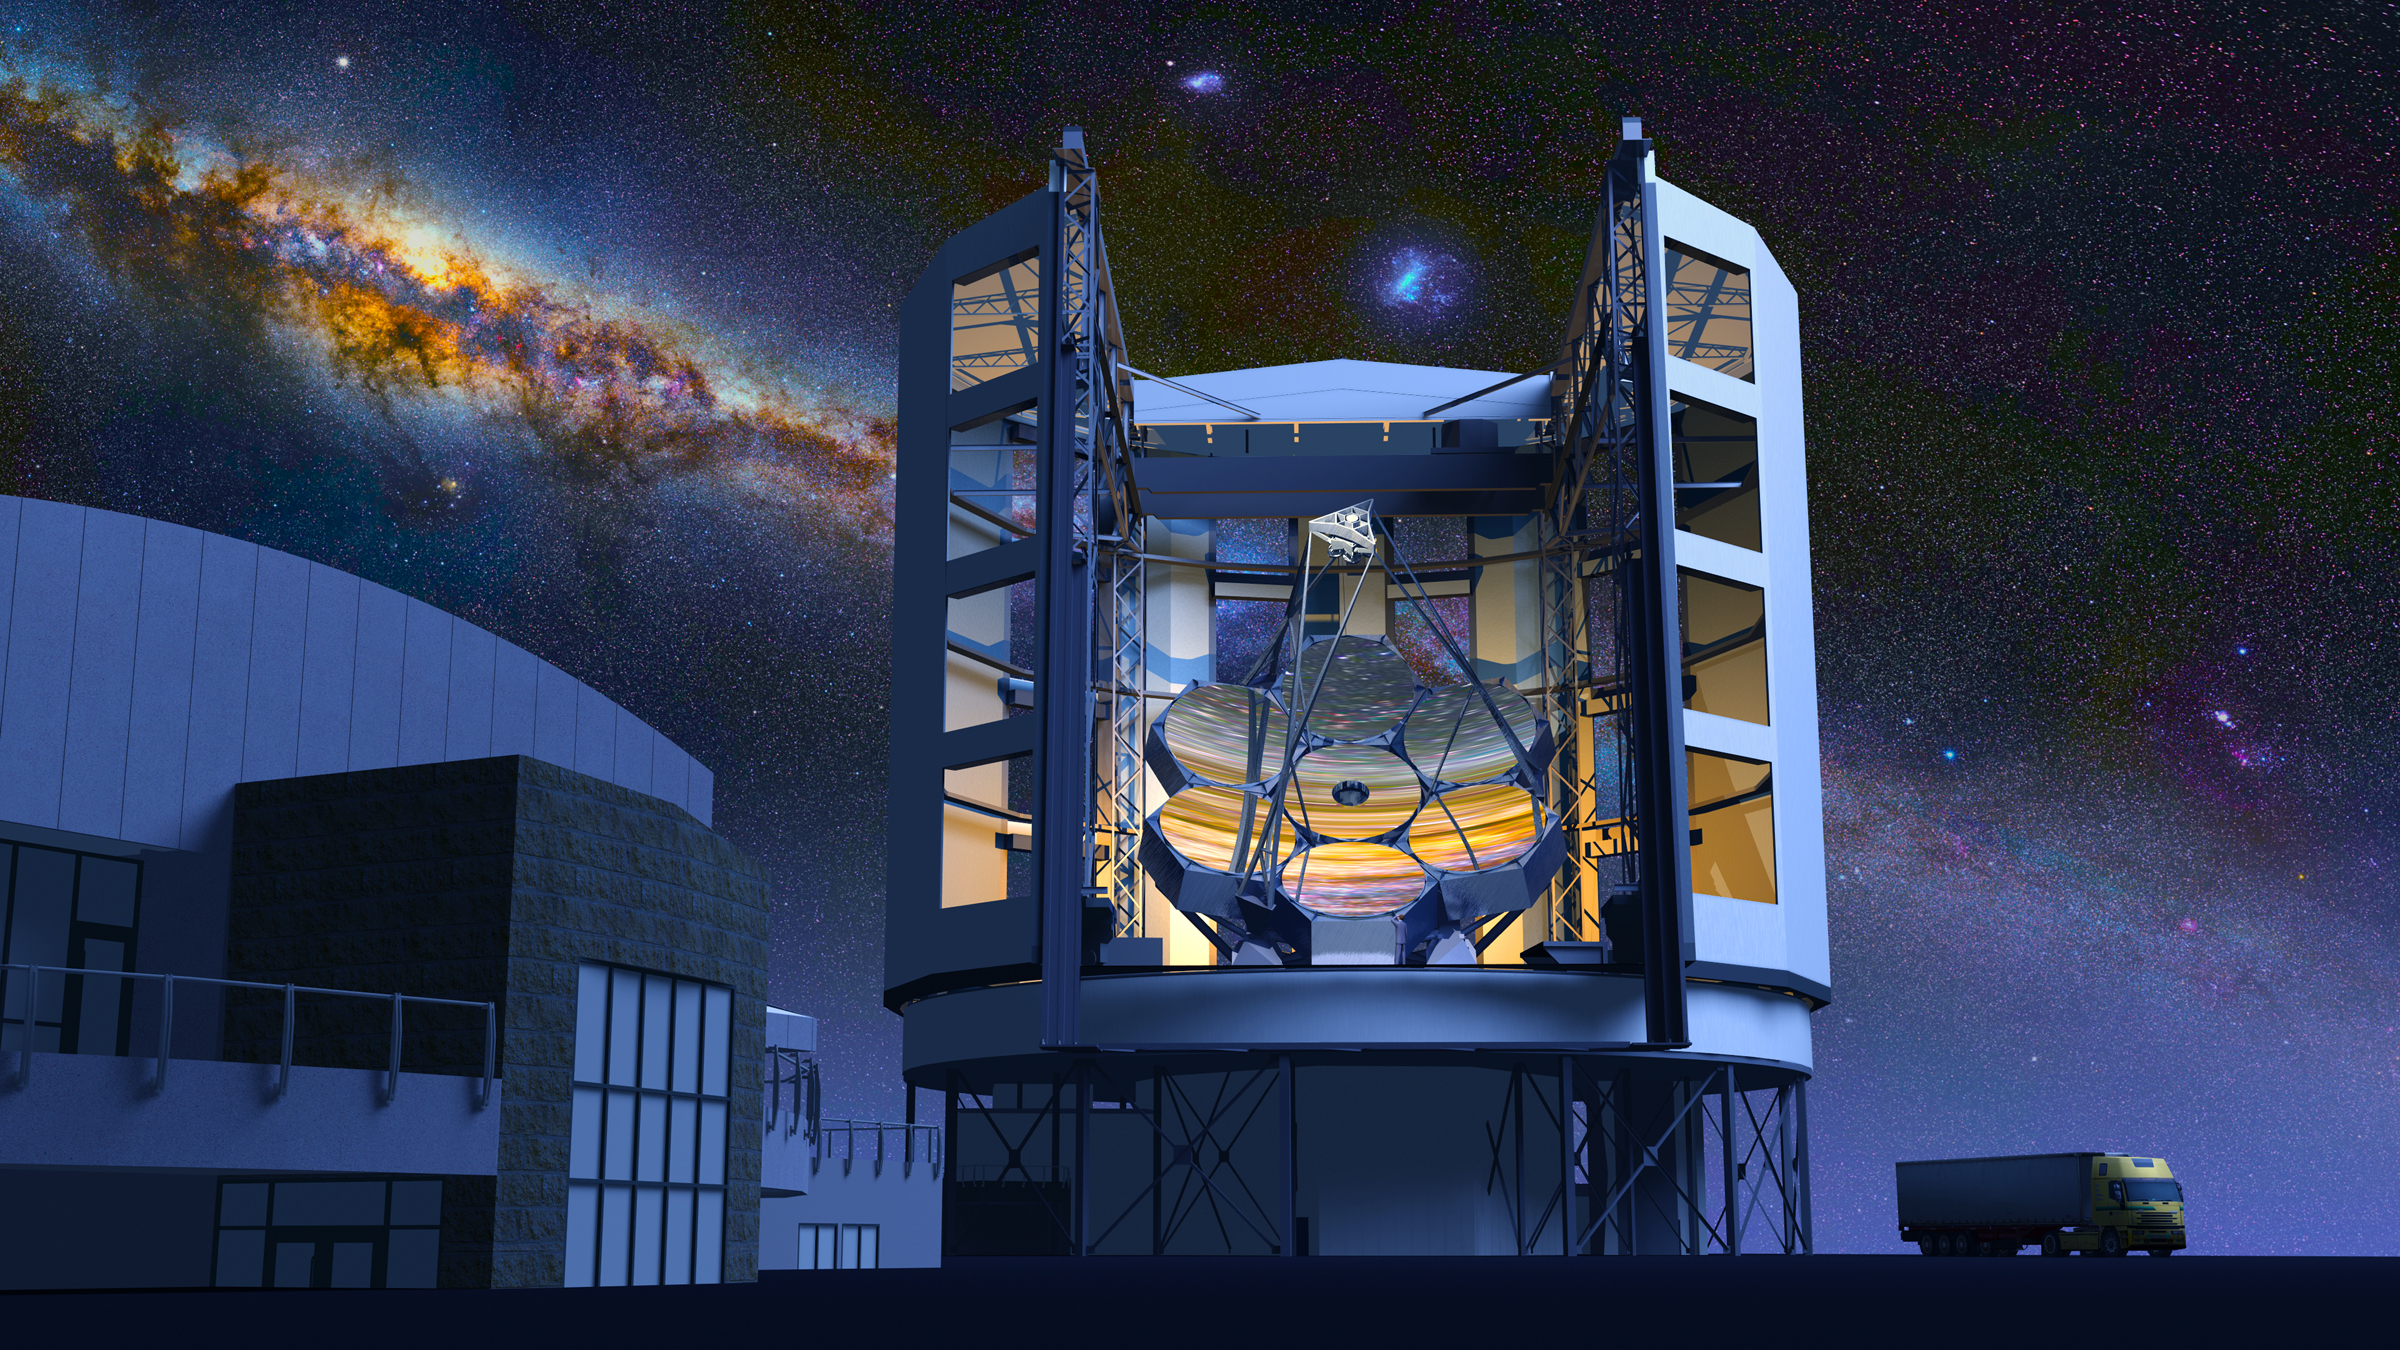
\includegraphics[width = .9\textwidth]{GMT}
\end{figure}

Per questi motivi l'attenuazione dei disturbi tramite sistemi di controllo attivo è oggi la tecnologia di riferimento per l'osservazione astronomica terrestre, e gli studi per l'applicazione spaziale sono in rapida diffusione.\\

Per quanto riguarda le applicazioni terrestri, in cui la principale fonte di disturbo è la diffrazione causata dalla turbolenza atmosferica, lo stato dell'arte è rappresentato, in particolar modo, dai due modelli in fase di sviluppo qui riportati:
\begin{description}
 \item[GMT] -- \textit{Giant Magellan Telescope}
 \item[E-ELT] -- \textit{European Extremely Large Telescope}
\end{description}

Il primo, frutto della collaborazione di diversi enti e università e finanziato principalmente da Australia, USA e Korea, vanterà un parco di 7 specchi primari di diametro di 8.4 m con un potere risolutivo equivalente a quello di un singolo specchio di 24 m.
L'ottica adattiva sarà installata sullo specchio secondario (M2) di 3.1 m.
Il telescopio sarà operativo presso l'osservatorio di Las Campanas (Cile) nel 2018.\\



Il secondo, nato da un progetto ESO (\textit{European Southern Observatory}), sarà situato a Cerro Amazones (Cile) e vanterà un diametro dello specchio primario (M1) di 39 m e un sistema complessivo di 5 specchi, di cui uno attivo (M4) di diametro pari a 2.6 m. 
L'anno di realizzazione previsto è il 2024.

\begin{figure}[htb]
\centering
\caption{E-ELT design concept (\textcopyright\url{www.eso.org})}
\label{fig:EELT}
\includegraphics[width = .9\textwidth]{EELT}
\end{figure}




L'ottica adattiva compensa le aberrazioni del fronte d'onda in ingresso attraverso il controllo della deformazione di uno o più componenti ottici (specchi) del telescopio. 
In figura \ref{fig:control_global} è riportata la struttura di un sistema ottico attivo \citep{manetti_high_2010}:
\begin{itemize}
\item Attraverso un sistema di guide laser viene misurata la distorsione del fronte d'onda;
\item  Sulla base dell'elaborazione dell'aberrazione, un controllore ottico calcola la forma di riferimento che dovrà assumere l'elemento deformabile (adattivo);
\item La deformazione desiderata viene inviata al sistema di controllo strutturale dello specchio;
\item Attraverso un elevato numero di attuatori e sensori il controllore impone allo specchio l'inseguimento della forma desiderata, in modo tale da compensare l'aberrazione del fronte d'onda e garantire la cancellazione dei diversi rumori.
\end{itemize}
\begin{figure}[htb]
\centering
\caption{Struttura del sistema di controllo complessivo}
\label{fig:control_global}
\resizebox{\textwidth}{!}{%
\begin{tikzpicture}[scale = .5]
    \draw[->] {(-4.75,.5) -- (-2.5,.5)};
    \draw  (-2.25,.5) circle (.25);
    \draw[->] {(-2,.5) -- (0,.5)};
    \draw (0,0) -- (2,0) -- (2,1) -- (0,1) -- (0,0);
    \draw[->] {(2,.5) -- (3.7,.5)};
    \draw (3.7,0) -- (6,0) -- (6,1) -- (3.7,1) -- (3.7,0);
    \draw[->] {(6,.5) -- (8,.5)};
    \draw (8,0) -- (10.5,0) -- (10.5,1) -- (8,1) -- (8,0);
    \draw {(10.5,.5) -- (11,.5)};
    \draw {(11,.5) -- (11,-3.5)};
    \draw {(11,-3.5) -- (-2.25,-3.5)};
    \draw[->] {(-2.25,-3.5) -- (-2.25,.25)};
    \draw {(10.25,0) -- (10.25,-3)};
    \draw {(10.25,-3) -- (8.25,-3)};
    \draw[->] {(8.25,-3) -- (8.25,0)};
    \draw (-2.35,.8) node[left] {+}; %label
    \draw (-2.15,.1) node[right] {--}; %label
    \tikzset{block/.append style={align = center , text width=10em,font=\tiny}}
    \draw (-4,1.2) node[block] {Fronte d'onda\\ distorto};
    \draw (1,0.5) node[block] {Sensore\\ d'onda};
    \draw (4.85,0.5) node[block] {Controllore\\ ottico};
    \draw (9.25,0.5) node[block] {Specchio\\ deformabile};
    \draw (9.25,-1.5) node[block] {Anelllo di \\ controllo\\ dello\\ specchio};
    \draw (-1,1.2) node[block] {Fronte d'onda\\ corretto};
    \draw (2.825,1.2) node[block] {Distorsione\\ residua};
    \draw (7,1.2) node[block] {Comando di\\ forma};
\end{tikzpicture}}
\end{figure}
\section{Elementi del sistema}

Lo specchio, che costituisce l'elemento strutturale deformabile, è una piastra sottile sospesa al di sopra di un corpo di riferimento rigido (\textit{reference body}). L'unico collegamento fra i due elementi è il sostegno centrale dello specchio il cui scopo è fornire un'elevata rigidezza nel piano e una modica rigidezza legata a movimenti trasversali. La distanza fra lo specchio sospeso e il riferimento è dell'ordine di $10^{-4}$ m. 

\begin{SCfigure}[2][htb]
\centering
\caption{Specchio deformabile di uno dei quattro telescopi che compongono il \textit{Very Large Telescope}, realizzato da ESO e situato a Cerro Paranal (\textcopyright\url{www.eso.org})}
\label{fig:shellVLT}
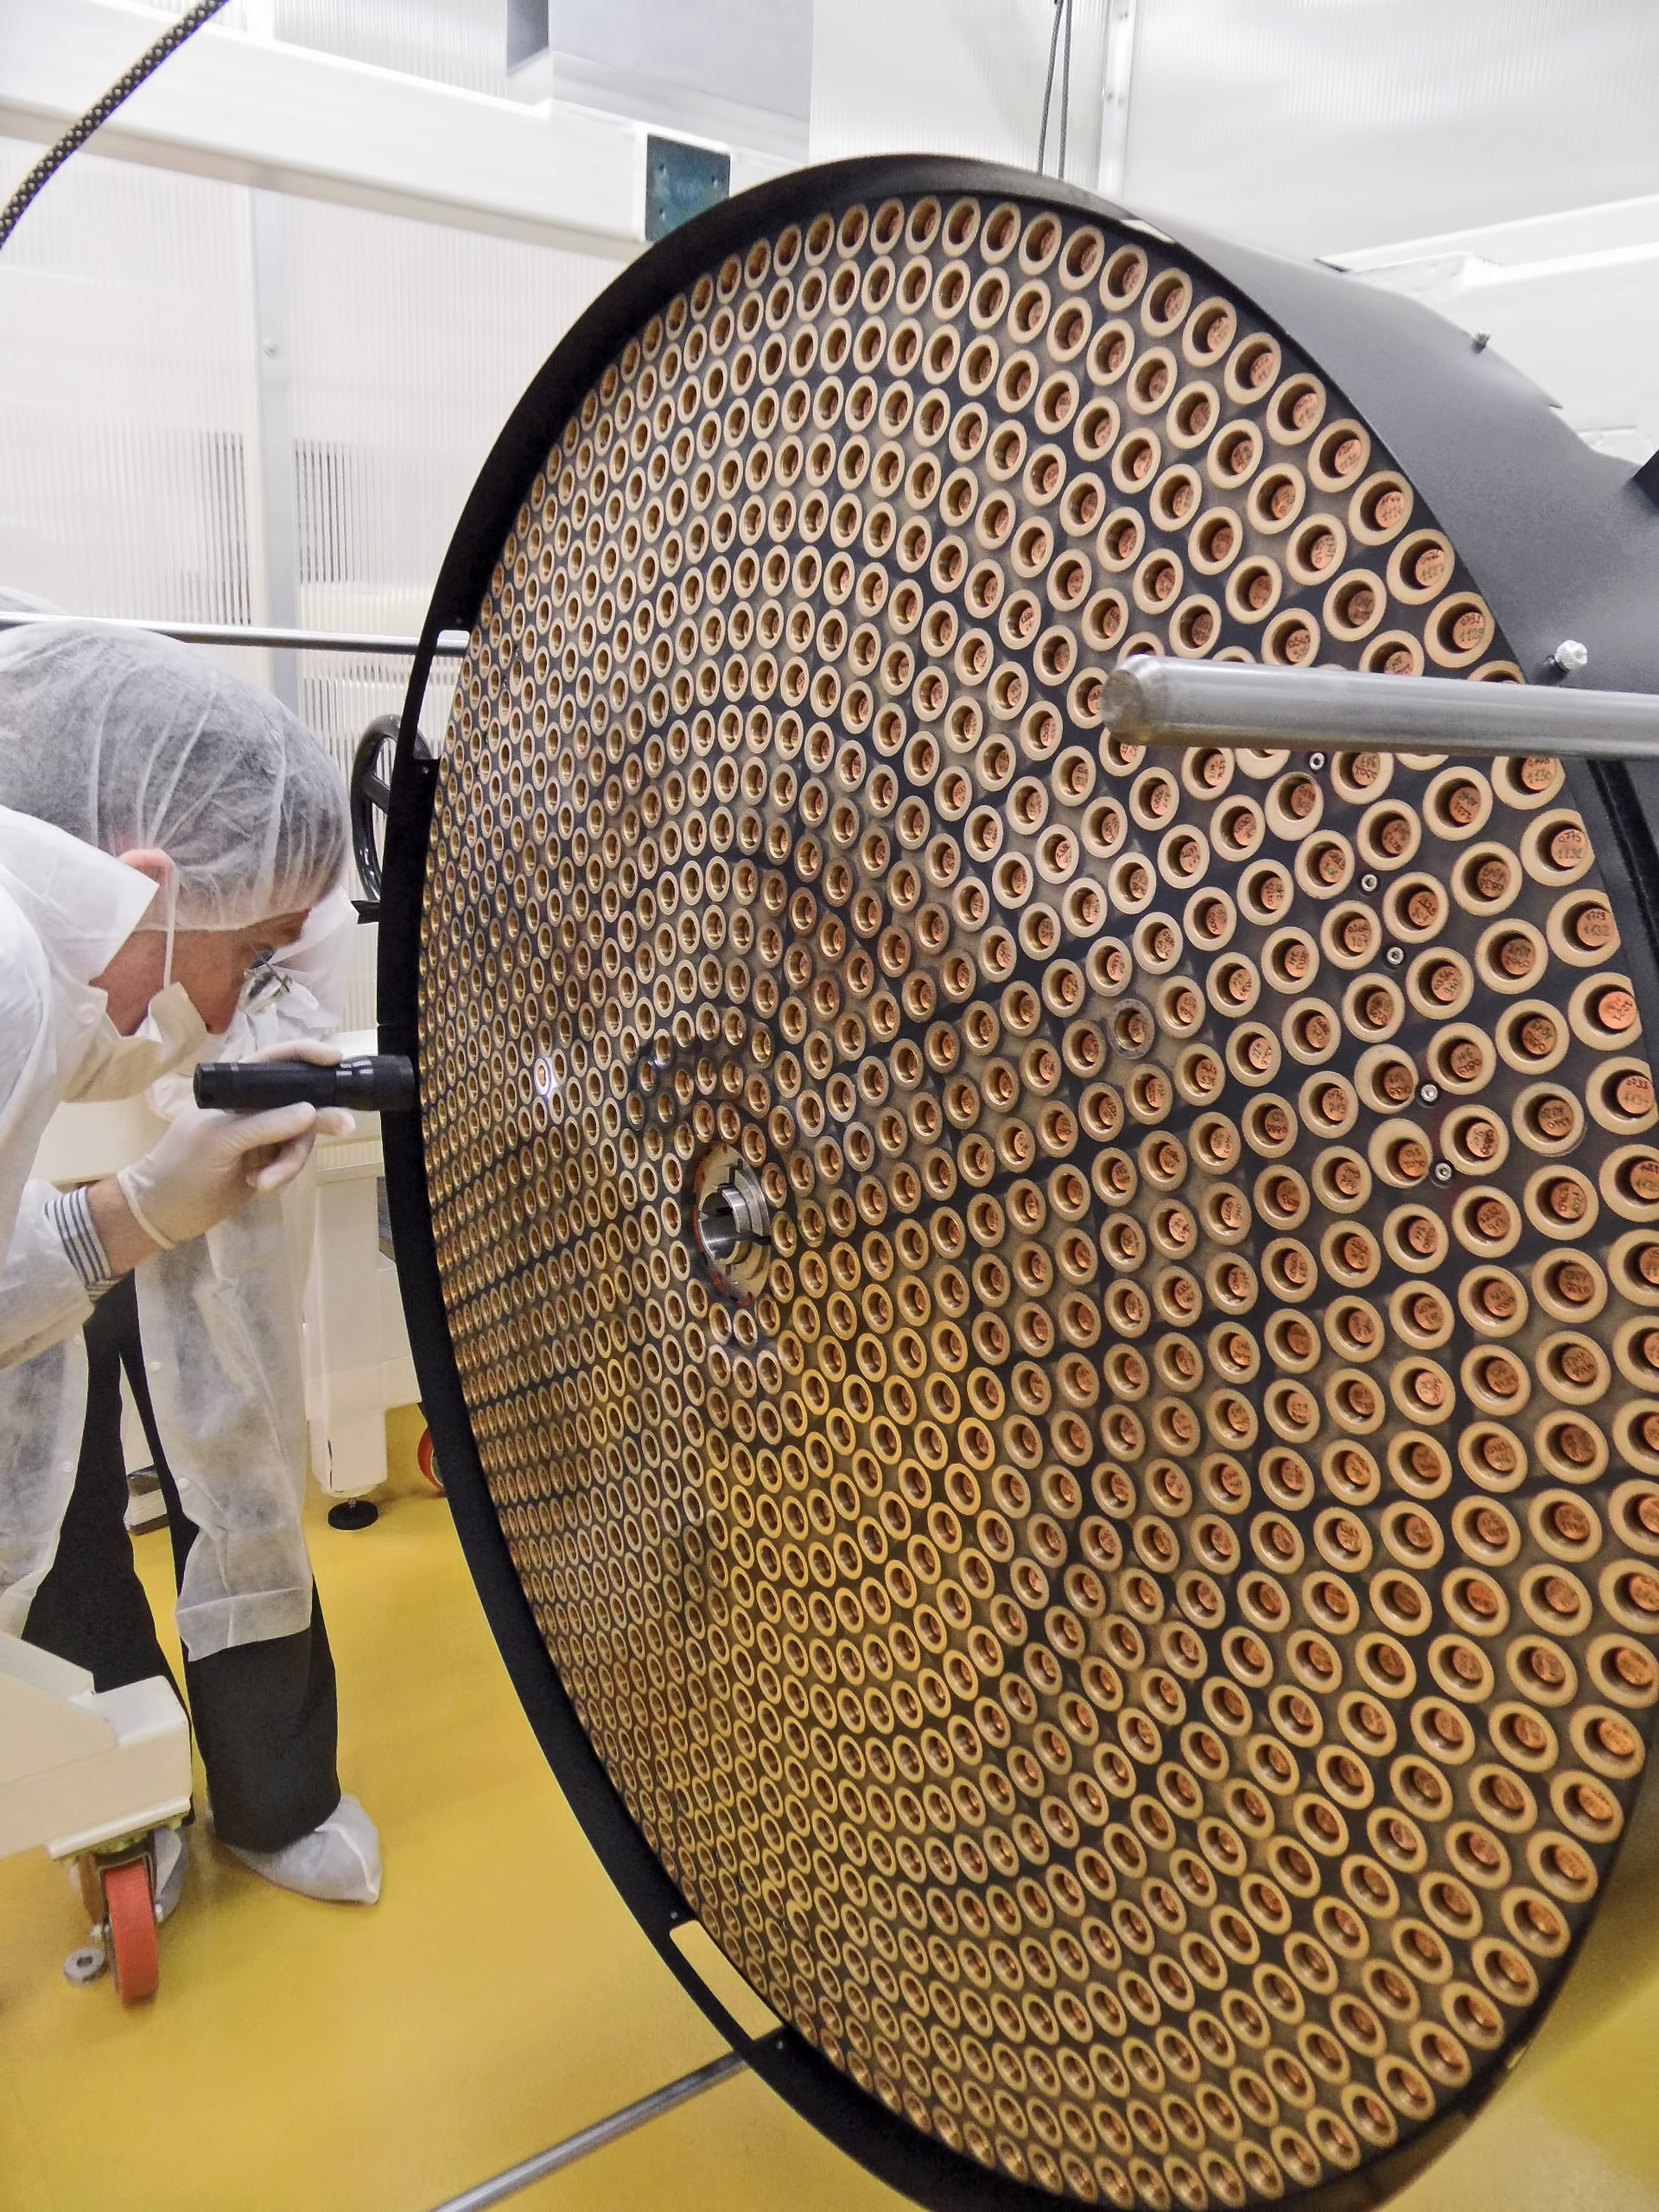
\includegraphics[width = .5\textwidth]{shellVLT}
\end{SCfigure}

Il reference body e lo specchio ospitano un gran numero di attuatori lineari a induzione collegati al sistema di controllo. Ciascun attuatore è circondato da un sensore capacitivo a corona circolare che permette la misura locale della distanza fra i due corpi. 

Il principio di attuazione è la forza magnetica scambiata fra un induttore solidale al reference body e un magnete permanente solidale alla piastra. 


Il sistema dinamico è formato da:
\begin{itemize}
\item Piastra deformabile
\item Reference body
\item Attuatori
\item Sensori
\end{itemize}

Sia per l'attuazione che per l'acquisizione le caratteristiche degli strumenti devono essere ben caratterizzate in funzione delle condizioni in cui operano. Particolare attenzione viene posta alla variazione del loro comportamento meccanico (in termini di forze e coppie) ed elettro-magnetico (induttanze, capacità e flussi concatenati) in funzione di posizione e rotazione relative degli elementi. 

Queste, a loro volta, dipendono da diversi fattori fra i quali: forma locale assunta dallo specchio, tolleranze di assemblaggio, disallineamenti dovuti a gravità e gradienti termici.

Lo scopo di questa tesi è l'analisi tramite simulazioni numeriche del comportamento degli attuatori e dei sensori adottati per il controllo dello specchio in funzione delle condizioni sopra citate e dell'impatto di questi ultimi nella simulazione del sistema controllato dello specchio di un telescopio. 

\begin{figure}[htb]
\centering
\caption{Reference body del Very Large Telescope (\textcopyright\url{www.eso.org})}
\label{fig:refVLT}
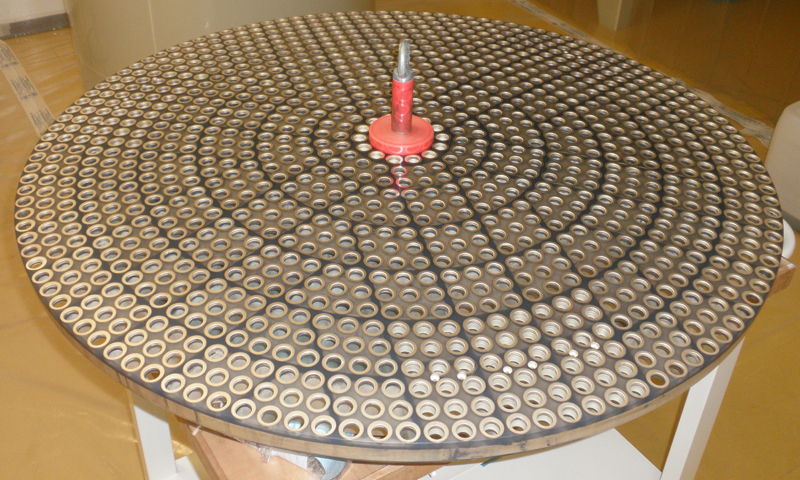
\includegraphics[width = .9\textwidth]{refVLT}
\end{figure}
\section{Strumenti utilizzati}
\'E stata fatta la scelta di effettuare tutte le simulazioni con il linguaggio di programmazione \textit{Python}, utilizzando le librerie dedicate al calcolo numerico \textit{numpy} \citep{numpy}, l'insieme di \textit{tool} grafici \textit{matplotlib} \citep{Hunter:2007} e soprattutto l'ambiente \textit{FEniCS} \citep{LoggMardalEtAl2012a} - in particolare il pacchetto \textit{Dolfin} \citep{LoggWellsEtAl2012a} - versatile insieme di librerie dedicate alla risoluzione di equazioni differenziali mediante il metodo agli elementi finiti. Punto di forza di FEniCS è la possibilità di risolvere problemi differenziali complessi sulla base dell'espressione del problema in forma debole e della griglia di calcolo (\textit{mesh}). \\

Il pacchetto permette di eseguire agevolmente le operazioni di assemblaggio delle matrici e di estrapolazione dei risultati. Per questo è stato scelto come strumento principale sia per le analisi elettromagnetiche (grazie anche alla possibilità di utilizzare la classe di elementi di Nèdèlèc) sia per le analisi strutturali (così da integrare direttamente il controllore in forma digitale rimanendo nello stesso ambiente di sviluppo). 

Per la generazione delle griglie di calcolo è stato utilizzato il programma \textit{Gmsh} \citep{gmsh}. 

Infine, le operazioni di \textit{post-processing} - laddove non sono state effettuate tramite Fenics - hanno richiesto l'utilizzo del programma \textit{Paraview} \citep{paraview}.\\ 

Tutti gli strumenti utilizzati sono open-source.\\

\begin{center}
\begin{tabular}{c}
\toprule
     
\includegraphics[width = .5\textwidth]{python-banner}\\
     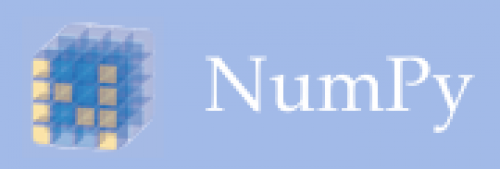
\includegraphics[width = .5\textwidth]{numpy-banner}\\
     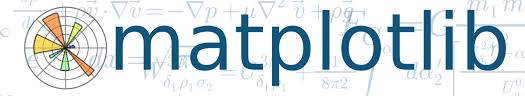
\includegraphics[width = .5\textwidth]{matplotlib-banner}\\
     
\includegraphics[width = .5\textwidth, height = .1\textwidth]{fenics-banner}\\
     
\includegraphics[width = .5\textwidth]{gmsh-banner}\\
     
\includegraphics[width = .5\textwidth]{paraview-banner}\\
\bottomrule
\end{tabular}
\end{center}
\section{Organizzazione del lavoro}


\begin{description}
\item[Nella prima parte] sono illustrati e validati i modelli matematici utilizzati per le analisi elettromagnetiche. In particolare:
  \begin{description}
  \item[Nel Capitolo \ref{cap:maxwell}] dopo aver richiamato brevemente le equazioni di Maxwell, vengono analizzati i modelli costitutivi, i regimi ridotti e gli schemi a potenziale.
  \item[Nel Capitolo \ref{cap:boundary}] sono elencate le condizioni al contorno e di interfaccia implementate. Viene inoltre mostrato lo sviluppo di una tecnica di trasformazione al contorno per l'analisi in domini aperti. Infine si verifica l'applicabilità delle ipotesi adottate per le condizioni al contorno nelle regioni metalliche. 
  \item[Nel Capitolo \ref{cap:bvp}] è illustrata la costruzione della forma variazionale del problema elettromagnetico e la conseguente scelta delle classi di elementi finiti adatte alla simulazione numerica.
  \item[Nel Capitolo \ref{cap:output}] viene posta attenzione al calcolo di forze e coppie, induttanze, flussi concatenati e capacità.
  \end{description}
\item[Nella seconda parte] si utilizzano i modelli sviluppati per l'analisi di un gruppo sensore-attuatore in fase di sviluppo. Viene inoltre generato un modello strutturale dello specchio per una valutazione del loro impatto sulle prestazioni del sistema di controllo. Più in dettaglio:
  \begin{description}
  \item[Nel Capitolo \ref{chap:ActSens}] vengono mostrati i risultati ottenuti per il gruppo di controllo preso in esame, analizzando forze e coppie scambiate, induttanze, flussi concatenati e capacità. 
  \item[Nel Capitolo \ref{chap:mirror}] vengono brevemente introdotti lo sviluppo del modello strutturale di uno specchio, la struttura del sistema di controllo e l'algoritmo di integrazione diretta nel tempo.
  \item[Nel Capitolo \ref{chap:simulations}] è analizzato l'effetto della modellazione di attuatori e sensori sulla simulazione diretta nel tempo della dinamica dello specchio durante l'inseguimento di una storia della durata di un secondo. Vengono proposte soluzioni per una migliore ricostruzione della velocità dei punti di controllo per un aumento della robustezza del sistema. Infine, viene impostato il controllo in tensione con controreazione proporzionale in corrente come alternativa al controllo in corrente.
  \item[Il Capitolo \ref{chap:Conclusioni}] riassume brevemente le conclusioni del lavoro e gli sviluppi futuri.
  \end{description}
\end{description}




\cleardoublepage\part{Costruzione e validazione dei modelli elettromagnetici}
% !TEX encoding = UTF-8 Unicode
% !TEX TS-program = pdflatex
% !TEX root = ../Tesi.tex


%************************************************
\myChapter{Il problema elettromagnetico}
%************************************************
\label{cap:maxwell}

\section{Equazioni di Maxwell}

La simulazione numerica elettromagnetica implica la risoluzione delle \textit{equazioni di Maxwell}, qui richiamate in forma puntuale:

\begin{equation}
	\label{eq:2max1}
	\rot\left(\T{e}\right)=-\partial_t \T{b},
\end{equation}

\begin{equation}
	\label{eq:2max2}
	\dive\left(\T{d}\right)=\rho,
\end{equation}

\begin{equation}
	\label{eq:2max3}
	\rot\left(\T{h}\right)=\T{j}+\partial_t \T{d},
\end{equation}

\begin{equation}
	\label{eq:2max4}
	\dive\left(\T{b}\right)=0,
\end{equation}
dove $\T{e} \; \left( \frac{\text{V}}{\text{m}} \right)$ e $\T{h} \; \left( \frac{\text{A}}{\text{m}} \right)$ sono rispettivamente le intensità di campo elettrico e magnetico, mentre $\T{d} \; \left( \frac{\text{C}}{\text{m}^2} \right)$ e $\T{b} \; \left( \frac{\text{Wb}}{\text{m}^2} \right)$ sono i vettori induzione elettrica e magnetica. 
\begin{SCfigure}[1.8][htp]
\caption{Superficie di riferimento per il teorema di Stokes, utilizzato nelle Eq. \eqref{eq:2faraday} e \eqref{eq:2ampere2}}
\label{fig:2.1}
\tdplotsetmaincoords{55}{45}
\begin{tikzpicture}
	[scale=2,
		tdplot_main_coords,
		curve/.style={draw = black,fill = black!10!white, opacity = .7}]
\def\R{.8} % sphere radius
\coordinate (O) at (0,0,0);
\coordinate (A) at (0,0,1);
\coordinate (B) at (0,\R,0);
\coordinate (C) at (0,0,-1);
%draw the circle in the main frame
\tdplotdrawarc[curve]{(O)}{\R}{0}{360}{}{}
\draw[->] {(O) -- (A)};
\draw (A) node[right] {$\T{n}$}; %label
\draw (\R*.4,0,0) node[right] {$S$}; %label
\draw (0, \R, 0) node[right] {$\partial S$}; %label
\end{tikzpicture}
\end{SCfigure}

L'equazione \eqref{eq:2max1} ha come forma integrale la \textit{legge di Faraday} (o \textit{legge dell'induzione elettromagnetica})che lega la circuitazione dell'intensità di campo elettrico lungo una linea chiusa alla variazione di flusso di induzione magnetica attraverso la superficie racchiusa:
\begin{equation}
\label{eq:2faraday}
\int_{\partial S} \T{e}\cdot d\T{l} = -\partial_t \int_S \T{b} \cdot d\T{s}.
\end{equation}

\begin{SCfigure}[2.5][htp]
\caption{Volume di riferimento per il teorema di Gauss, utilizzato in Eq. \eqref{eq:2gauss}}
\label{fig:2.2}
\begin{tikzpicture}
    \draw (-2,0) arc (180:360:2cm and 1cm);
    \draw[dashed] (-2,0) arc (180:0:2cm and 1cm);
    \draw (0,2) arc (90:270:1cm and 2cm);
    \draw[dashed] (0,2) arc (90:-90:1cm and 2cm);
    \draw (0,0) circle (2cm);
    \shade[ball color=black!10!white,opacity=0.20] (0,0) circle (2cm);
    \draw[->] {(1,1) -- (2,2)};
    \draw (2,2) node[right] {$\T{n}$}; %label
    \draw (-1.8,0.5) node[left] {$\partial V$}; %label
    \draw (-.6,-1.5) node[right] {$V$}; %label
\end{tikzpicture}\end{SCfigure}

L'equazione \eqref{eq:2max2} è il \textit{teorema di Gauss} applicato al campo elettrico:
\begin{equation}
\label{eq:2gauss}
\int_{\partial V} \T{d} \cdot d\T{s}= Q_{enc} = \int_V \rho dv,
\end{equation}
dove $Q_{enc}$ è la carica totale racchiusa nel volume $V$ circondato dalla superficie $\partial V$, e $\rho$ è la densità di carica per unità di volume.
\\
L'equazione \eqref{eq:2max3} è il risultato della modifica apportata da Maxwell alla \textit{legge di  Ampère}, in origine:
\[
\int_{\partial S} \T{h} \cdot d\T{l} = i_{enc} = \int_S \T{j} \cdot d\T{s},
\]
dove $i_{enc}$ è la corrente totale che attraversa la superficie $S$, e $\T{j}$ è la densità di corrente per unità di superficie (\textit{corrente volumetrica}).

Il termine $\partial_t \T{d}$ (che Maxwell ha nominato \textit{corrente di spostamento}) porta alla simmetria delle equazioni e alla forma integrale:
\begin{equation}
\label{eq:2ampere2}
\int_{\partial S} \T{h} \cdot d\T{l} = \int_S \left( \T{j} + \partial_t \T{d} \right) \cdot d\T{s}.
\end{equation}

Infine l'equazione \eqref{eq:2max4} rappresenta la solenoidalità dell'induzione magnetica $\T{b}$:
\begin{equation}
\label{eq:2solen}
\int_{\partial V} \T{b} \cdot d\T{s} = 0.
\end{equation}

Si noti che applicando la divergenza ad entrambi i termini dell'equazione \eqref{eq:2max3} si può ottenere il legame tra cariche e correnti elettriche. Questo legame è pertanto implicito nella definizione del problema:
\begin{align}
\label{eq:2corr1}
\dive \left[ \rot\left(\T{h}\right) \right] &= \dive \left(\T{j}+\partial_t \T{d} \right) \nonumber\\
0&=\dive \left(\T{j}\right) + \partial_t \dive \left(\T{d}\right) \nonumber\\
0&=\dive \left(\T{j}\right) + \partial_t\rho\nonumber\\
\partial_t \rho &= - \dive \left(\T{j}\right).
\end{align}

\section{Legami costitutivi}

Per definire le interazioni fra le diverse equazioni occorre indagare i legami tra le intensità di campo e le rispettive induzioni; tali relazioni dipendono dalla natura del dominio in cui vengono applicate le equazioni. 

Nel vuoto si hanno le ben note relazioni:
\begin{equation}
\label{eq:2cost}
\left\{
\begin{aligned}
\T{d} &= \varepsilon_0 \T{e}\\
\T{b} &= \mu_0 \T{h}
\end{aligned}
\qquad\text{con}\qquad
\begin{aligned}
\varepsilon_0&=8{,}854\,187\,817\,62\cdot 10^{-12} &\frac{\text{F}}{\text{m}}\\
\mu_0&= 1{,}256\,637\,061\,44\cdot10^{-6} &\frac{\text{H}}{\text{m}}
\end{aligned}
\right.
\end{equation}

A queste si aggiunga la relazione tra il campo elettrico all'interno di un materiale e la corrente generata all'interno dello stesso (\textit{conduction current}):
\begin{equation}
\label{eq:2conduction_current}
\T{j}=\T{j_c}+\T{j_i}, \qquad \text{con}\qquad \T{j_c}=\sigma \T{e}
\end{equation}
dove $\T{j_i}$ è la \textit{corrente impressa} e $\sigma$ è la conduttività del materiale. 

Nel vuoto si ha:
\[
\sigma=0
\]
Nei prossimi paragrafi verrà brevemente giustificata la natura delle leggi costitutive in seguito utilizzate.


\subsection{Campi elettrici nella materia}
\label{subsec:elecmateria}
La risposta di un materiale alle sollecitazioni del campo elettrico varia in base alla natura del materiale stesso. 

Identifichiamo due grandi classi di materiali: \textit{isolanti} (o \textit{dielettrici}) e \textit{conduttori}. In un materiale isolante ciascun elettrone è legato ad uno specifico atomo, mentre in un conduttore gli elettroni (o gli ioni per i conduttori liquidi) sono liberi di spostarsi fra i diversi nuclei.
\begin{itemize}
\item[\textit{Isolanti}]
Quando un materiale dielettrico viene sottoposto ad un campo elettrico ciascun atomo (neutro) è sottoposto ad una forza totale nulla; tuttavia nuclei ed elettroni sono sottoposti a forze uguali ed opposte, a causa della loro carica non nulla tali forze tendono quindi ad allontanare nucleo ed elettroni. Eccezion fatta per i casi in cui tale forza è così alta da separarli completamente (ionizzando l'atomo) viene raggiunta una nuova configurazione di equilibrio tra le forze interne di attrazione fra nucleo ed elettroni e le forze indotte dal campo elettrico esterno. 

In questa configurazione l'atomo è detto \textit{polarizzato} e possiede un momento di dipolo $\T{p_a}$  parallelo al campo elettrico e ad esso proporzionale tramite la \textit{polarizzabilità} $\alpha$:
\begin{equation}
\label{eq:2polar1}
\T{p} = \alpha \left(\T{e}\right)\cdot \T{e}.
\end{equation}

Considerando intere molecole anziché singoli atomi la polarizzazione può seguire direzioni preferenziali e non essere pertanto parallela al campo elettrico.
Più in generale si ha quindi:
\begin{equation}
\label{eq:2polar2}
\T{p_m} = \TT{\alpha} \left( \T{e} \right) \cdot\T{e},
\end{equation}
dove $\TT{\alpha}$ è un tensore del II ordine (tensore di polarizzabilità).
In questa configurazione il campo elettrico esterno esercita una coppia sulle molecole che tende ad allineare i dipoli con il campo stesso:
\begin{equation}
\label{eq:2polar3}
\T{C_p}=\T{p_m} \times \T{e}.
\end{equation}

Il campo elettrico esercita quindi due azioni sulle molecole: distorsione e rotazione. Entrambe portano allo stesso risultato: il dielettrico presenta un numero di dipoli allineati in una direzione preferenziale.

Definiamo quindi per un materiale dielettrico il vettore $\T{p}$ (\textit{polarizzazione}) come la densità di momenti di dipolo. Questo campo è la sintesi dell'effetto che le cariche generate dal campo elettrico esterno esercitano sul campo elettrico stesso.
Le cariche sono esprimibili tramite il vettore di polarizzazione come:
\begin{equation}
\label{eq:2charges1}
\left\{
\begin{aligned}
\rho_{b} &= -\dive \left(\T{p}\right) \qquad &\text{in $V$}\\
\sigma_{b} &= \T{p}\cdot \T{n} \qquad &\text{in $S$}.
\end{aligned}
\right.
\end{equation}
 
Riscrivendo l'equazione \eqref{eq:2gauss} nel dominio del materiale, utilizzando la prima delle \eqref{eq:2cost} e aggiungendo le cariche dovute alla polarizzazione si ha:
\begin{align}
\label{eq:2polar3}
&\int_S \varepsilon_0\T{e} \cdot d\T{s}  = \int_V \left( \rho+\rho_{b}\right) dv\nonumber\\
&\int_S \varepsilon_0\T{e} \cdot d\T{s}  = \int_V \left[ \rho-\dive\left(\T{p}\right)\right] dv\nonumber\\
&\int_V \dive\left[\varepsilon_0\T{e} + \T{p} \right]\cdot dv  = \int_V \rho dv,\nonumber
\end{align}
da cui:
\begin{equation}
\label{eq:2polar4}
\T{d} = \varepsilon_0 \T{e} + \T{p}\left(\T{e}\right).
\end{equation}

Un caso comune è quello in cui la polarizzazione è proporzionale al campo elettrico:
\begin{equation}
\label{eq:2polar5}
\T{p} = \varepsilon_0 \TT{\chi_e} \T{e},
\end{equation}
dove  il tensore del II ordine $\TT{\chi_e}$ è detto \textit{suscettibilità elettrica}.

L'equazione \eqref{eq:2polar4} porta a:
\begin{equation}
\begin{split}
\label{eq:2polar6}
\T{d} &= \left[\varepsilon_0 \TT{I}+ \TT{\chi_e}\left(\T{e}\right)\right]\T{e} \\
      &= \TT{\varepsilon}\T{e}.
\end{split}
\end{equation}

Per materiali con proprietà dielettriche isotrope si può considerare il campo $\T{p}$ sempre parallelo a $\T{e}$. 

In questo caso si può scrivere:
\begin{equation}
\begin{split}
\label{eq:2costel}
\T{d} &= \left[\varepsilon_0+ \chi_e\left(\T{e}\right)\right]\T{e} \\
      &= \varepsilon\T{e}.
\end{split}
\end{equation}
\item[\textit{Conduttori}] La relazione \eqref{eq:2conduction_current} è applicabile a tutti i materiali, ma assume un ruolo non trascurabile solo se la conduttività del materiale è rilevante. Maggiore è $\sigma$ minore è il campo elettrico all'interno del materiale (in assenza di correnti impresse).
Al limite, identifichiamo come conduttore elettrico perfetto (\textit{Perfect Electric Conductor, PEC}) il materiale per cui:
\begin{equation}
\label{eq:2pec}
\sigma \rightarrow \infty,\qquad \T{e}\rightarrow 0.
\end{equation}
Questo modello è utile per rappresentare adeguatamente regioni metalliche che non costituiscono zone d'interesse per l'analisi; queste possono essere quindi escluse dal dominio di analisi e sostituite con adeguate condizioni al contorno. 
Nel caso in cui sia di primario interesse lo sviluppo dei campi elettromagnetici all'interno del conduttore (ad esempio nell'analisi di correnti parassite) il materiale deve essere adeguatamente modellato ed incluso nel dominio di analisi: 
\begin{align}
\label{eq:2pec2}
\T{d} &= \varepsilon\T{e},\\
\T{j} &= \T{j_i}+\sigma\T{e}.
\end{align}
Esistono tuttavia modelli semplificati adeguati all'analisi specifica di questa classe di problemi \citep{zaglmayr_high_2006}.
\end{itemize}
\subsection{Campi magnetici nella materia}
Proprietà analoghe possono essere mostrate anche per la controparte magnetica.

Gli elettroni appartenenti agli atomi di un materiale non magnetizzato, in quanto cariche in movimento dal periodo estremamente basso possono essere rappresentati come correnti stazionarie (lungo le loro orbite) di intensità:
\begin{equation}
\label{eq:2current1}
i=\frac{e}{T}=\frac{e v}{2 \pi R}.
\end{equation}

Si ricorda che una spira percorsa da corrente stazionaria è soggetta ad un momento meccanico:
\begin{equation}
\T{\tau}=\T{m}\times\T{b}, 
\end{equation}
\label{eq:2torque}
dove $\T{m}$ è detto \textit{momento di dipolo magnetico} ed è dato da
\begin{equation}
\label{eq:2mom}
\T{m}=i S \T{\hat{z}} = -\frac{1}{2}evR\T{\hat{z}}\quad \text{($S$ è la superficie racchiusa dall'orbita).}
\end{equation}
\begin{SCfigure}[2.4][htp]
\caption{Orbita di un elettrone attorno al nucleo e relativo momento di dipolo magnetico}
\label{fig:2.3}
\tdplotsetmaincoords{55}{45}
\begin{tikzpicture}
	[scale=2,
		tdplot_main_coords,
		curve/.style={draw = black,fill = black!10!white, opacity = .7},
		curve2/.style={black,->}]
\def\R{.8} % sphere radius
\coordinate (O) at (0,0,0);
\coordinate (A) at (0,0,1);
\coordinate (B) at (0,\R,0);
\coordinate (C) at (0,0,-1);
%draw the circle in the main frame
\draw[->] {(O) -- (C)};
\draw (C) node[right] {$\T{m}$}; %label
\tdplotdrawarc[curve]{(O)}{\R}{0}{360}{}{}
\tdplotdrawarc[curve2]{(O)}{\R*1.2}{320}{400}{}{}
\draw[->] {(O) -- (A)};
\draw[->] {(O) -- (B)};
\draw (A) node[right] {$\T{\hat{z}}$}; %label
\draw (B) node[right] {$-e$}; %label
\draw (\R*1.3,0,0) node[right] {$v$}; %label
\draw (0, \R/2, 0) node[right] {$R$}; %label
\end{tikzpicture}
\end{SCfigure}

La normale all'orbita dell'elettrone tende pertanto ad allinearsi con il campo magnetico.

In analogia con la polarizzazione, definiamo qui la \textit{magnetizzazione} $\T{m}\left(\T{h}\right)$ come la densità di momenti di dipolo magnetico.

Gli effetti dovuti alla magnetizzazione possono essere riassunti in una distribuzione di correnti equivalenti, volumetriche e superficiali:
\begin{equation}
\label{eq:2current2}
\left\{
\begin{aligned}
\T{j_{b}} &= \rot \left(\T{m}\right) \qquad &\text{in $V$}\\
\T{k_{b}} &= \T{m}\times \T{\hat{n}} \qquad &\text{in $S$}.
\end{aligned}
\right.
\end{equation}

Scriviamo ora il teorema di Ampère (Eq. \eqref{eq:2ampere2}) utilizzando il legame costitutivo \eqref{eq:2cost}:
\begin{align}
\label{eq:2current3}
&\oint_L \frac{1}{\mu_0}\T{b} \cdot d\T{l}  = \int_S \left( \T{j}+\T{j_{b}}+\partial_t\T{d}\right) d\T{s}\nonumber\\
&\oint_L \frac{1}{\mu_0}\T{b} \cdot d\T{l}  = \int_S \left( \T{j}+\rot\left(\T{m}\right)+\partial_t\T{d}\right) d\T{s}\nonumber\\
&\int_S \rot\left(\frac{1}{\mu_0}\T{b}-\T{m}\right) \cdot d\T{s}  = \int_S \left( \T{j}+\partial_t\T{d}\right) d\T{s},
\end{align}
che porta alla relazione costitutiva per il materiale magnetizzato:

\begin{equation}
\label{eq:2current4}
\T{b}=\mu_0\left(\T{h}+\T{m}\right).
\end{equation}

La natura di $\T{m}$ dipende fortemente dal tipo di materiale cui si fa riferimento. Si può assumere che in base al loro comportamento, i materiali di più comune interesse ricadano in una delle seguenti categorie \citep{furlani_permanent_2001}:
\begin{description}
\item[Paramagnetici]Gli atomi o le molecole di questi materiali hanno un momento netto, ma non vi è relazione fra le direzioni dei momenti adiacenti. Se sottoposti ad un campo magnetico i momenti tendono ad allinearvisi; l'allineamento è randomatico e dipende dall'intensità del campo applicato; diminuisce inoltre con l'aumento di temperatura.
\item[Ferromagnetici] Come per i materiali paramagnetici, gli atomi o le molecole dei materiali ferromagnetici hanno un momento netto; vi è però un forte accoppiamento fra momenti adiacenti che ne provoca l'allineamento spontaneo in regioni limitate dette \textit{domini}. Se sottoposti ad un campo magnetico esterno i momenti di questi domini non variano sensibilmente (localmente $\T{m}>>\T{h_{ext}}$); la magnetizzazione di ciascun dominio si allinea tuttavia con il campo esterno, dando origine ad un campo di magnetizzazione complessivo molto elevato. Al di sopra di una temperatura caratteristica per ciascun materiale (\textit{temperatura di Curie}) il comportamento torna paramagnetico.
\item[Antiferromagnetici] Anche per questi materiali vi è un accoppiamento fra i momenti di atomi o molecole adiacenti all'interno di domini distinti; la disposizione assunta, tuttavia, è di antiparallelismo; il momento magnetico netto è quindi nullo.
\item[Ferrimagnetici]Come per i materiali antiferromagnetici i momenti adiacenti sono antiparalleli; l'intensità è tuttavia in questo caso maggiore in un verso che nell'altro e si origina così un momento netto non nullo.
\item[Diamagnetici] Il diamagnetismo è un fenomeno di natura quantistica comune a tutti i materiali e molto debole; sono detti materiali diamagnetici quelli in cui non vi è nessun altro comportamento dominante.

Rientrano in questa categoria i materiali che non hanno un momento magnetico atomico o molecolare netto. Se sottoposti ad un campo esterno sviluppano una magnetizzazione debole ed opposta al campo applicato. Esempi di questi materiali sono l'acqua, le sostanze organiche e alcuni metalli (oro, argento, bismuto, mercurio).
\end{description}

\begin{figure}[htp]
\centering
\caption{Momenti magnetici nei diversi materiali}
\label{fig:2.4}
\subfloat[][Paramagnetici]{
\begin{tikzpicture}
\filldraw[fill = black!20!white, draw = black] (0,0) rectangle (.31\textwidth,.16\textwidth);
\draw[->] (.15\textwidth,.01\textwidth) -- (.18\textwidth,.02\textwidth);
\draw[->] (.23\textwidth,.14\textwidth) -- (.24\textwidth,.11\textwidth);
\draw[->] (.01\textwidth,.02\textwidth) -- (.04\textwidth,.01\textwidth);
\draw[->] (.02\textwidth,.14\textwidth) -- (.02\textwidth,.11\textwidth);
\draw[->] (.17\textwidth,.10\textwidth) -- (.14\textwidth,.09\textwidth);
\draw[->] (.10\textwidth,.07\textwidth) -- (.11\textwidth,.10\textwidth);
\draw[->] (.24\textwidth,.01\textwidth) -- (.22\textwidth,.03\textwidth);
\draw[->] (.26\textwidth,.06\textwidth) -- (.29\textwidth,.06\textwidth);
\draw[->] (.20\textwidth,.09\textwidth) -- (.22\textwidth,.07\textwidth);
\draw[->] (.09\textwidth,.13\textwidth) -- (.06\textwidth,.13\textwidth);
\draw[->] (.06\textwidth,.09\textwidth) -- (.03\textwidth,.08\textwidth);
\draw[->] (.10\textwidth,.02\textwidth) -- (.09\textwidth,.05\textwidth);
\draw[->] (.15\textwidth,.12\textwidth) -- (.16\textwidth,.15\textwidth);
\draw[->] (.17\textwidth,.05\textwidth) -- (.14\textwidth,.06\textwidth);
\draw[->] (.30\textwidth,.12\textwidth) -- (.27\textwidth,.13\textwidth);
\end{tikzpicture}
}
\subfloat[][Ferromagnetici]{
\begin{tikzpicture}
\filldraw[fill = black!20!white, draw = black] (0,0) rectangle (.31\textwidth,.16\textwidth);
\draw[->] (.01\textwidth,.02\textwidth) -- (.06\textwidth,.02\textwidth);
\draw[->] (.07\textwidth,.02\textwidth) -- (.12\textwidth,.02\textwidth);
\draw[->] (.13\textwidth,.02\textwidth) -- (.18\textwidth,.02\textwidth);
\draw[->] (.19\textwidth,.02\textwidth) -- (.24\textwidth,.02\textwidth);
\draw[->] (.25\textwidth,.02\textwidth) -- (.30\textwidth,.02\textwidth);

\draw[->] (.01\textwidth,.04\textwidth) -- (.06\textwidth,.04\textwidth);
\draw[->] (.07\textwidth,.04\textwidth) -- (.12\textwidth,.04\textwidth);
\draw[->] (.13\textwidth,.04\textwidth) -- (.18\textwidth,.04\textwidth);
\draw[->] (.19\textwidth,.04\textwidth) -- (.24\textwidth,.04\textwidth);
\draw[->] (.25\textwidth,.04\textwidth) -- (.30\textwidth,.04\textwidth);

\draw[->] (.01\textwidth,.06\textwidth) -- (.06\textwidth,.06\textwidth);
\draw[->] (.07\textwidth,.06\textwidth) -- (.12\textwidth,.06\textwidth);
\draw[->] (.13\textwidth,.06\textwidth) -- (.18\textwidth,.06\textwidth);
\draw[->] (.19\textwidth,.06\textwidth) -- (.24\textwidth,.06\textwidth);
\draw[->] (.25\textwidth,.06\textwidth) -- (.30\textwidth,.06\textwidth);

\draw[->] (.01\textwidth,.08\textwidth) -- (.06\textwidth,.08\textwidth);
\draw[->] (.07\textwidth,.08\textwidth) -- (.12\textwidth,.08\textwidth);
\draw[->] (.13\textwidth,.08\textwidth) -- (.18\textwidth,.08\textwidth);
\draw[->] (.19\textwidth,.08\textwidth) -- (.24\textwidth,.08\textwidth);
\draw[->] (.25\textwidth,.08\textwidth) -- (.30\textwidth,.08\textwidth);

\draw[->] (.01\textwidth,.10\textwidth) -- (.06\textwidth,.10\textwidth);
\draw[->] (.07\textwidth,.10\textwidth) -- (.12\textwidth,.10\textwidth);
\draw[->] (.13\textwidth,.10\textwidth) -- (.18\textwidth,.10\textwidth);
\draw[->] (.19\textwidth,.10\textwidth) -- (.24\textwidth,.10\textwidth);
\draw[->] (.25\textwidth,.10\textwidth) -- (.30\textwidth,.10\textwidth);

\draw[->] (.01\textwidth,.12\textwidth) -- (.06\textwidth,.12\textwidth);
\draw[->] (.07\textwidth,.12\textwidth) -- (.12\textwidth,.12\textwidth);
\draw[->] (.13\textwidth,.12\textwidth) -- (.18\textwidth,.12\textwidth);
\draw[->] (.19\textwidth,.12\textwidth) -- (.24\textwidth,.12\textwidth);
\draw[->] (.25\textwidth,.12\textwidth) -- (.30\textwidth,.12\textwidth);

\draw[->] (.01\textwidth,.14\textwidth) -- (.06\textwidth,.14\textwidth);
\draw[->] (.07\textwidth,.14\textwidth) -- (.12\textwidth,.14\textwidth);
\draw[->] (.13\textwidth,.14\textwidth) -- (.18\textwidth,.14\textwidth);
\draw[->] (.19\textwidth,.14\textwidth) -- (.24\textwidth,.14\textwidth);
\draw[->] (.25\textwidth,.14\textwidth) -- (.30\textwidth,.14\textwidth);
\end{tikzpicture}
}\\
\subfloat[][Antiferromagnetici]{
\begin{tikzpicture}
\filldraw[fill = black!20!white, draw = black] (0,0) rectangle (.31\textwidth,.16\textwidth);

\draw[->] (.06\textwidth,.02\textwidth) -- (.01\textwidth,.02\textwidth);
\draw[->] (.12\textwidth,.02\textwidth) -- (.07\textwidth,.02\textwidth);
\draw[->] (.18\textwidth,.02\textwidth) -- (.13\textwidth,.02\textwidth);
\draw[->] (.24\textwidth,.02\textwidth) -- (.19\textwidth,.02\textwidth);
\draw[->] (.30\textwidth,.02\textwidth) -- (.25\textwidth,.02\textwidth);

\draw[->] (.01\textwidth,.04\textwidth) -- (.06\textwidth,.04\textwidth);
\draw[->] (.07\textwidth,.04\textwidth) -- (.12\textwidth,.04\textwidth);
\draw[->] (.13\textwidth,.04\textwidth) -- (.18\textwidth,.04\textwidth);
\draw[->] (.19\textwidth,.04\textwidth) -- (.24\textwidth,.04\textwidth);
\draw[->] (.25\textwidth,.04\textwidth) -- (.30\textwidth,.04\textwidth);

\draw[->] (.06\textwidth,.06\textwidth) -- (.01\textwidth,.06\textwidth);
\draw[->] (.12\textwidth,.06\textwidth) -- (.07\textwidth,.06\textwidth);
\draw[->] (.18\textwidth,.06\textwidth) -- (.13\textwidth,.06\textwidth);
\draw[->] (.24\textwidth,.06\textwidth) -- (.19\textwidth,.06\textwidth);
\draw[->] (.30\textwidth,.06\textwidth) -- (.25\textwidth,.06\textwidth);

\draw[->] (.01\textwidth,.08\textwidth) -- (.06\textwidth,.08\textwidth);
\draw[->] (.07\textwidth,.08\textwidth) -- (.12\textwidth,.08\textwidth);
\draw[->] (.13\textwidth,.08\textwidth) -- (.18\textwidth,.08\textwidth);
\draw[->] (.19\textwidth,.08\textwidth) -- (.24\textwidth,.08\textwidth);
\draw[->] (.25\textwidth,.08\textwidth) -- (.30\textwidth,.08\textwidth);

\draw[->] (.06\textwidth,.10\textwidth) -- (.01\textwidth,.10\textwidth);
\draw[->] (.12\textwidth,.10\textwidth) -- (.07\textwidth,.10\textwidth);
\draw[->] (.18\textwidth,.10\textwidth) -- (.13\textwidth,.10\textwidth);
\draw[->] (.24\textwidth,.10\textwidth) -- (.19\textwidth,.10\textwidth);
\draw[->] (.30\textwidth,.10\textwidth) -- (.25\textwidth,.10\textwidth);

\draw[->] (.01\textwidth,.12\textwidth) -- (.06\textwidth,.12\textwidth);
\draw[->] (.07\textwidth,.12\textwidth) -- (.12\textwidth,.12\textwidth);
\draw[->] (.13\textwidth,.12\textwidth) -- (.18\textwidth,.12\textwidth);
\draw[->] (.19\textwidth,.12\textwidth) -- (.24\textwidth,.12\textwidth);
\draw[->] (.25\textwidth,.12\textwidth) -- (.30\textwidth,.12\textwidth);

\draw[->] (.06\textwidth,.14\textwidth) -- (.01\textwidth,.14\textwidth);
\draw[->] (.12\textwidth,.14\textwidth) -- (.07\textwidth,.14\textwidth);
\draw[->] (.18\textwidth,.14\textwidth) -- (.13\textwidth,.14\textwidth);
\draw[->] (.24\textwidth,.14\textwidth) -- (.19\textwidth,.14\textwidth);
\draw[->] (.30\textwidth,.14\textwidth) -- (.25\textwidth,.14\textwidth);
\end{tikzpicture}
}
\subfloat[][Ferrimagnetici]{
\begin{tikzpicture}
\filldraw[fill = black!20!white, draw = black] (0,0) rectangle (.31\textwidth,.16\textwidth);
\draw[->] (.04\textwidth,.02\textwidth) -- (.03\textwidth,.02\textwidth);
\draw[->] (.10\textwidth,.02\textwidth) -- (.09\textwidth,.02\textwidth);
\draw[->] (.16\textwidth,.02\textwidth) -- (.15\textwidth,.02\textwidth);
\draw[->] (.22\textwidth,.02\textwidth) -- (.21\textwidth,.02\textwidth);
\draw[->] (.28\textwidth,.02\textwidth) -- (.27\textwidth,.02\textwidth);

\draw[->] (.01\textwidth,.04\textwidth) -- (.06\textwidth,.04\textwidth);
\draw[->] (.07\textwidth,.04\textwidth) -- (.12\textwidth,.04\textwidth);
\draw[->] (.13\textwidth,.04\textwidth) -- (.18\textwidth,.04\textwidth);
\draw[->] (.19\textwidth,.04\textwidth) -- (.24\textwidth,.04\textwidth);
\draw[->] (.25\textwidth,.04\textwidth) -- (.30\textwidth,.04\textwidth);

\draw[->] (.04\textwidth,.06\textwidth) -- (.03\textwidth,.06\textwidth);
\draw[->] (.10\textwidth,.06\textwidth) -- (.09\textwidth,.06\textwidth);
\draw[->] (.16\textwidth,.06\textwidth) -- (.15\textwidth,.06\textwidth);
\draw[->] (.22\textwidth,.06\textwidth) -- (.21\textwidth,.06\textwidth);
\draw[->] (.28\textwidth,.06\textwidth) -- (.27\textwidth,.06\textwidth);

\draw[->] (.01\textwidth,.08\textwidth) -- (.06\textwidth,.08\textwidth);
\draw[->] (.07\textwidth,.08\textwidth) -- (.12\textwidth,.08\textwidth);
\draw[->] (.13\textwidth,.08\textwidth) -- (.18\textwidth,.08\textwidth);
\draw[->] (.19\textwidth,.08\textwidth) -- (.24\textwidth,.08\textwidth);
\draw[->] (.25\textwidth,.08\textwidth) -- (.30\textwidth,.08\textwidth);

\draw[->] (.04\textwidth,.10\textwidth) -- (.03\textwidth,.10\textwidth);
\draw[->] (.10\textwidth,.10\textwidth) -- (.09\textwidth,.10\textwidth);
\draw[->] (.16\textwidth,.10\textwidth) -- (.15\textwidth,.10\textwidth);
\draw[->] (.22\textwidth,.10\textwidth) -- (.21\textwidth,.10\textwidth);
\draw[->] (.28\textwidth,.10\textwidth) -- (.27\textwidth,.10\textwidth);

\draw[->] (.01\textwidth,.12\textwidth) -- (.06\textwidth,.12\textwidth);
\draw[->] (.07\textwidth,.12\textwidth) -- (.12\textwidth,.12\textwidth);
\draw[->] (.13\textwidth,.12\textwidth) -- (.18\textwidth,.12\textwidth);
\draw[->] (.19\textwidth,.12\textwidth) -- (.24\textwidth,.12\textwidth);
\draw[->] (.25\textwidth,.12\textwidth) -- (.30\textwidth,.12\textwidth);

\draw[->] (.04\textwidth,.14\textwidth) -- (.03\textwidth,.14\textwidth);
\draw[->] (.10\textwidth,.14\textwidth) -- (.09\textwidth,.14\textwidth);
\draw[->] (.16\textwidth,.14\textwidth) -- (.15\textwidth,.14\textwidth);
\draw[->] (.22\textwidth,.14\textwidth) -- (.21\textwidth,.14\textwidth);
\draw[->] (.28\textwidth,.14\textwidth) -- (.27\textwidth,.14\textwidth);
\end{tikzpicture}
}
\end{figure}

Per materiali  diamagnetici e paramagnetici isotropi la magnetizzazione è in genere parallela e proporzionale ad $\T{h}$:
\begin{equation}
\label{eq:2magnetiz1}
\T{m} = \chi \T{h}
\end{equation}
\begin{equation}
\label{eq:2magnetiz2}
\T{b}= \mu_0 \left(1+\chi\right)\T{h} = \mu \T{h} .
\end{equation}

La costante di proporzionalità $\chi$ è detta \textit{suscettività elettrica}, dipende dalla temperatura ed è negativa per i diamagnetici e positiva per i paramagnetici; nella maggior parte dei casi è dell'ordine di $10^{-4}-10^{-5}$.

Nel caso di anisotropie nei materiali  $\chi$ e $\mu$  in Eq. \eqref{eq:2magnetiz2} diventano tensori del secondo ordine:
 \begin{equation}
\label{eq:2magnetiz3}
\T{m} = \TT{\chi} \T{h}
\end{equation}
\begin{equation}
\label{eq:2magnetiz4}
\T{b}= \mu_0 \left(\TT{I}+\TT{\chi}\right)\T{h} = \TT{\mu} \T{h} .
\end{equation}


Per la caratterizzazione della legge costitutiva nei materiali ferromagnetici è necessaria l'analisi della loro  natura isteretica. In fig. \ref{fig:2.4} è mostrato un tipico grafico $\T{h}~-~\T{b}$ per un materiale a comportamento isteretico.

\begin{figure}[htp]
\centering
\caption{Curva di isteresi magnetica}
\label{fig:2.5}
\begin{tikzpicture}
\begin{axis}[ylabel = $\T{b}\left(\T{h}\right)$,
			 xlabel = $\T{h}$,
			 ticks = none, 
			 ymax = 1100,
			 axis x line = middle, 
			 axis y line = middle, 
			 enlargelimits,
			 semithick]
\addplot[samples = 100, smooth, domain=-40:40]
{10*atan(x-10)};
\addplot[samples = 100, smooth, domain=-40:40]
{10*atan(x+10)};
\addplot[samples = 100, smooth, domain=0:40]
{(5*atan(0.8*(x-7))-5*atan(-0.8*7))*10*atan(30)/(5*atan(0.8*30)-5*atan(-0.8*7))};
\draw (-2.5,80) node {$O$}; %label
\draw (40,980) node {$S$}; %label
\draw (2.5,940) node {$R$}; %label
\draw (-14,80) node {$C$}; %label
\end{axis}
\end{tikzpicture}
\end{figure}

Nel punto $O$ nessun campo magnetico $\T{h}$ è applicato e i momenti di dipolo all'interno dei domini hanno direzioni randomatiche ($\T{m} = 0$).  
Con l'applicazione di un campo magnetico esterno i domini tendono ad allinearvisi e il materiale si muove lungo la curva $O-S$ in cui l'induzione magnetica cresce con $\T{h}$. 

Nel punto $S$ il materiale è saturo e i tutti i domini sono allineati al campo applicato. Diminuendo $\T{h}$ il campo si muove lungo la linea $S-R$, poiché il campo generato dai  domini contribuisce a mantenerne l'allineamento. 

Nel punto $R$ il materiale è nella condizione operativa e possiede un'\textit{induzione residua} $\T{b_r}$. 
Per poter tornare ad induzione magnetica nulla è necessario applicare un campo di verso opposto, muovendosi fino al punto $C$, la cui ascissa è detta \textit{coercitività} ($\T{h_c}$).  Il materiale è quindi vincolato a muoversi lungo l'anello isteretico e non può tornare alla curva $O-S$.

I materiali ferromagnetici si classificano, a seconda delle loro caratteristiche di coercitività e permeabilità, in:
\begin{description}
\item[Materiali soffici] Questi materiali hanno alta permeabilità e bassa coercitività ($\T{h_c}<10^3 \frac{\text{A}}{\text{m}}$) e sono quindi facili da magnetizzare e smagnetizzare. 

Vengono pertanto usati come canali per condurre o amplificare il flusso magnetico in trasformatori, motori, elettromagneti, induttori, ecc.
\item[Materiali duri] Al contrario, questi materiali hanno permeabilità relativamente bassa, alta coercitività ($\T{h_c}>10^4 \frac{\text{A}}{\text{m}}$)e sono difficili da magnetizzare e smagnetizzare. Sono utilizzati pertanto come magneti permanenti.
\end{description}

\begin{figure}[htb]
\centering
\caption{Curva di isteresi: confronto fra materiali morbidi (linea continua) e duri (linea tratteggiata)}
\label{fig:2.6}
\begin{tikzpicture}
\begin{axis}[ylabel = $\T{b}\left(\T{h}\right)$,
			 xlabel = $\T{h}$,
			 ticks = none, 
			 ymax = 1100,
			 axis x line = middle, 
			 axis y line = middle, 
			 enlargelimits,
			 semithick]
\addplot[samples = 100, smooth, domain=-40:40]
{10*atan(x-1)};
\addplot[samples = 100, smooth, domain=-40:40]
{10*atan(x+1)};
\addplot[samples = 100, smooth, domain=-40:40, dashed, very thick]
{10*atan(x-25)};
\addplot[samples = 100, smooth, domain=-40:40, dashed, very thick]
{10*atan(x+25)};
\end{axis}
\end{tikzpicture}
\end{figure}

La tipica condizione operativa per i magneti morbidi è quella della ripida retta tra i due punti di saturazione inferiore e superiore. La linearità di questo tratto  e il valore estremamente basso di coercitività giustificano l'utilizzo delle relazioni \eqref{eq:2magnetiz1} e \eqref{eq:2magnetiz2} anche nel caso di materiali ferromagnetici, purché il campo applicato non sia eccessivo ($\T{b}< 1 \text{T}$, \citep{bossavit_computational_1998}). 
In questo caso $\chi$ varia tra $10^{3}$ e $10^{5}$.

Portando al limite le caratteristiche dei materiali magnetici soffici, si definisce il conduttore magnetico perfetto (\textit{perfect magnetic conductor, PMC}) come il materiale avente le seguenti proprietà:
\begin{equation}
\label{eq:2pmc}
\mu \rightarrow \infty,\qquad \T{h}\rightarrow 0.
\end{equation}

I magneti permanenti, magnetizzati durante il processo di produzione, hanno come condizione di riposo il punto $R$ di Figura \ref{fig:2.5} e in condizioni operative restano nell'intorno di questo punto (tratto lineare). Per questa classe di materiali è pertanto giustificato utilizzare il seguente modello:
\begin{align}
\label{eq:2costmag}
\T{m(h)}&=\TT{\chi}\T{h}+\T{m_r}\nonumber \\
\T{b(h)}&=\mu_0(\T{h}+\left(\TT{\chi}\T{h}+\T{m_r}\right) \nonumber\\
&=\mu_0\left(\TT{I}+\TT{\chi}\right)\T{h}+\mu_0 \T{m_r} \nonumber \\
&=\TT{\mu}\T{h}+\mu_0 \T{m_r}\nonumber\\
&= \TT{\mu}\T{h}+\T{b_r}.
\end{align}
\section{Regimi speciali}
Non sempre è necessario applicare il modello completo fornito dalle equazioni di Maxwell per la risoluzione di problemi di natura elettromagnetica. In molte applicazioni, infatti, la dinamica dei campi è parzialmente o interamente trascurabile perché più veloce della variazione delle condizioni al contorno associate. 

Vengono qui brevemente introdotti due modelli, adottati per le successive analisi.

\subsection{Regime quasi-stazionario magnetico}
A basse frequenze e se le dimensioni caratteristiche del problema sono molto inferiori alle lunghezze d'onda proprie del campo elettromagnetico si può applicare l'approssimazione quasi-stazionaria: in queste condizioni il campo elettromagnetico varia con tempi più lunghi di quelli necessari alla sua propagazione e si può pertanto assumere che la velocità di quest'ultima sia infinita (qualsiasi variazione nel campo elettromagnetico è percepita istantaneamente in tutto il dominio). I tre modelli quasi-stazionari più utilizzati sono \citep{larsson_electromagnetics_2007}:
\begin{itemize}
\item Modello quasi-stazionario magnetico (\textit{MQS})
\item Modello quasi-stazionario elettrico (\textit{EQS})
\item Modello di Darwin
\end{itemize}

Viene posta attenzione qui solo al regime \textit{MQS}, utilizzato nelle simulazioni successive.

Nel regime quasi-stazionario magnetico si presuppone che la variazione del campo $\partial_t \T{d}$ dia un contributo trascurabile rispetto alla corrente libera $\T{j}$; tale termine viene pertanto eliminato nell'equazione \eqref{eq:2max3}. Questo porta alla riscrittura delle equazioni \eqref{eq:2max1}-\eqref{eq:2max4}:
\begin{equation}
	\label{eq:2max1qs}
	\rot\left(\T{e}\right)=-\partial_t \T{b},
\end{equation}
\begin{equation}
	\label{eq:2max2qs}
	\dive\left(\T{d}\right)=\rho,
\end{equation}
\begin{equation}
	\label{eq:2max3qs}
	\rot\left(\T{h}\right)=\T{j},
\end{equation}
\begin{equation}
	\label{eq:2max4qs}
	\dive\left(\T{b}\right)=0,
\end{equation}
con
\begin{equation}
\label{eq:2corr1qs}
\dive\left(\T{j}\right) = 0.
\end{equation}

Dalla prima equazione si evince che il campo magnetico e la  sua induzione seguono staticamente la variazione temporale di corrente $\T{j}$ e non dipendono dalla controparte elettrica\footnote{In realtà i due campi continuano ad interagire laddove la corrente $\T{j}$ dipende dal campo elettrico. Particolare attenzione va posta, pertanto, nella corretta modellazione del comportamento delle regioni metalliche (Capitolo \ref{cap:boundary}).}. 
Il campo elettrico è invece influenzato separatamente nelle sue parti di rotore e divergenza dalle equazioni \eqref{eq:2max1qs} e \eqref{eq:2max2qs}.
Questa separazione suggerisce una scomposizione del campo $\T{e}$ in due parti:
\begin{equation}
\label{eq:2scomp_e}
\T{e} = \T{e_c}+\T{e_f},
\end{equation} 
dove $\T{e_c}$ è irrotazionale ed è identificato tramite la sola legge di Coulomb:
\begin{equation}
\label{eq:2e_coulomb}
\left\{
\begin{array}{l}
\dive\left(\TT{\varepsilon} \T{e_c}\right) = \rho\\
\rot\left(\T{e_c}\right) = 0
\end{array}
\right.
\end{equation}
e $\T{e_f}$ è solenoidale e segue la legge di Faraday:
\begin{equation}
\label{eq:2e_faraday}
\left\{
\begin{array}{l}
\dive\left(\TT{\varepsilon} \T{e_f}\right) = 0\\
\rot\left(\T{e_f}\right) =\partial_t \T{b}.
\end{array}
\right.
\end{equation}

Questa separazione suggerisce la seguente strategia di calcolo:
\begin{enumerate}
\item Risoluzione delle equazioni \eqref{eq:2max3qs} e \eqref{eq:2max4qs} per ottenere staticamente la storia temporale di $\T{b}$ e $\T{h}$ ;
\item Risoluzione della prima delle equazioni \eqref{eq:2e_coulomb} per la determinazione della parte irrotazionale di $\T{e}$ ($\T{e_c}$);
\item Determinazione della storia temporale di $\T{e_f}$ mediante la seconda delle \eqref{eq:2e_faraday}.
\end{enumerate}


\subsection{Regime stazionario}
In assenza completa di variazioni temporali si può ritenere nullo qualsiasi contributo dinamico. In questo caso anche il termine $\partial_t\T{b}$ è nullo e le equazioni sono pienamente disaccoppiate, permettendo lo studio separato di elettrostatica e magnetostatica.
\begin{equation}
\label{eq:2max12s}
\left\{
\begin{aligned}
\rot\left(\T{e}\right)=0\\
\dive\left(\T{d}\right)=\rho
\end{aligned}
\right.
\end{equation}
e
\begin{equation}
\label{eq:2max34s}
\left\{
\begin{aligned}
\rot\left(\T{h}\right)=\T{j}\\
\dive\left(\T{b}\right)=0.
\end{aligned}
\right.
\end{equation}
\subsection{Condizioni di applicabilità}
Dopo aver introdotto i diversi regimi ci chiediamo quali condizioni devono essere verificate perché la loro applicazione sia giustificata.
Un primo criterio di applicazione dei regimi quasi-stazionari \citep{zaglmayr_high_2006} è il confronto tra i tempi di propagazione delle onde elettromagnetiche all'interno del dominio di analisi e i tempi caratteristici di variazione delle sorgenti dei campi (cariche e correnti). In regime armonico si ha:
\begin{equation}
\label{eq:2regimi1}
\tau_{\lambda} = \frac{L}{c} \gg \frac{2\pi}{\omega_s} = \tau_s,
\end{equation}
dove $L$ è la dimensione caratteristica del dominio, $c$ è la velocità di propagazione delle onde e $\omega_s$ è la pulsazione caratteristica delle sorgenti di campo.\\

Si può tuttavia analizzare più approfonditamente l'ordine di grandezza delle quantità che possono venire trascurate nella scelta dei diversi regimi \citep{emson_methods_1988}; in quest'ottica approssimiamo le derivate spaziali e temporali utilizzando la lunghezza caratteristica $L$ e un tempo caratteristico $\tau$. 

Iniziamo cercando un criterio per discernere i campi di applicabilità dei regimi \textit{MQS} e dinamico. Chiamiamo $\hat{h}$ il campo che soddisfa l'Eq. \eqref{eq:2max3qs}:
\begin{equation}
\label{eq:2regimi2}
\hat{h} L = j L^2 \longrightarrow \hat{h} =  j L
\end{equation}   
e $h$ il campo che soddisfa l'Eq. \eqref{eq:2max3}:
\begin{equation}
\label{eq:2regimi3}
h =  j L +  \varepsilon \frac{e}{\tau} L.
\end{equation}

L'errore tra $\hat{h}$ e $h$ è dato da
\begin{equation}
\label{eq:2regimi4}
\Delta h =  \varepsilon \frac{e}{\tau},
\end{equation}
dove
\begin{equation}
\label{eq:2regimi5}
e L = \mu \frac{\hat{h}}{\tau} L^2 \longrightarrow e = \mu \frac{\hat{h}}{\tau} L.
\end{equation}

Si noti che è stato utilizzato $\hat{h}$ in Eq. \eqref{eq:2regimi5} e non $h$. Si ottiene così una stima dell'errore:
\begin{align}
\label{eq:2regime6_a}
\Delta h = \mu \varepsilon j \frac{L^3}{\tau^2}, \\
\label{eq:2regime6_b}
\frac{\Delta h}{\hat{h}} = \mu \varepsilon \frac{L^2}{\tau^2}.
\end{align}

Se $\Delta h$ è trascurabile rispetto a $\hat{h}$ è ragionevole l'utilizzo dell'approccio \textit{MQS}.\\

Cerchiamo ora una stima dell'intensità di campo elettrico indotta dalla variazione di induzione magnetica, utile per avere un criterio di scelta fra regime \textit{MQS} e regime stazionario:
\begin{align}
\label{eq:2regimi7_a}
hL= jL^2 \longrightarrow \frac{h}{L} &= j\\
\label{eq:2regimi7_b}
eL= \frac{b}{\tau} L^2 \longrightarrow\frac{e}{L} &= \frac{\mu h}{\tau},
\end{align} 
da cui
\begin{equation}
\label{eq:2regimi8}
e = \frac{\mu j L^2}{\tau}.
\end{equation}

Se tale valore è piccolo il modello stazionario è applicabile con buona approssimazione.\\

Per dimostrare l'applicabilità del regime MQS ed avere una stima dell'errore commesso, il criterio sopra mostrato è stato verificato per dimensioni e tempi conservativi rispetto a quelli tipici per gli attuatori del sistema di controllo:
\begin{equation}
\nonumber
\begin{array}{l}
L = 0.1 \text{m},\\
\tau = 10^-5 \text{s}.
\end{array}
\end{equation}
Si ottiene:
\begin{equation}
\nonumber
\begin{array}{l}
\frac{\Delta h}{\hat{h}} = 10^{-6},\\
e = 10^{-3}j.
\end{array}
\end{equation}
Guardando il primo dei due termini si può ritenere appropriato l'utilizzo del regime quasi-stazionario in sostituzione al regime dinamico completo. Tuttavia l'ordine di grandezza del campo elettrico non permette di stabilire a priori l'applicabilità del regime stazionario completo.

\section{Potenziale scalare e potenziale vettore}
\label{subsec:1potenziale}
\subsection{Regime dinamico}
Scegliamo ora una formulazione che permetta di soddisfare a priori la solenoidalità del campo $\T{b}$ (Eq. \eqref{eq:2max4}). Introduciamo quindi il \textit{potenziale vettore} $\T{a}$ tale per cui
\begin{equation}
\label{eq:2potvet}
\rot\left(\T{a}\right) = \T{b}.
\end{equation}

Sostituendo nell'equazione \eqref{eq:2max1} l'induzione magnetica secondo la relazione di cui sopra, si ottiene:
\begin{align}
\label{eq:2potvet2}
\rot\left(\T{e}\right)=-\partial_t \rot\left(\T{a}\right)\nonumber\\
\rot\left(\T{e}\right)=- \rot\left(\partial_t\T{a}\right)\nonumber\\
\rot\left(\T{e}+\partial_t\T{a}\right)=0.
\end{align}


Poiché la quantità $\T{e}+\partial_t\T{a}$ è irrotazionale è possibile introdurre un secondo potenziale, questa volta \textit{scalare}, $\phi$:
\begin{equation}
\label{eq:2potsca}
\T{e}+\partial_t\T{a} = - \grad\left(\phi\right)
\end{equation}
da cui
\begin{equation}
\label{eq:2potsca2}
\T{e} = - \grad\left(\phi\right)-\partial_t\T{a}
\end{equation}

Possiamo quindi ora riscrivere le Eq. \eqref{eq:2max2} e \eqref{eq:2max3}, utilizzando i potenziali appena definiti, utilizzando le leggi costitutive \eqref{eq:2costel} e \eqref{eq:2costmag}:
\begin{align}
\label{eq:2pot1}
\dive\left(\T{d}\right)&=\rho\nonumber\\
\dive\left(\TT{\varepsilon}\T{e}\right) &= \rho \nonumber\\
\dive \left[ \TT{\varepsilon} \cdot \grad \left( \phi \right) \right] + \dive \left[ \TT{\varepsilon} \partial_t \left( \T{a} \right) \right] &= -\rho \nonumber\\
\dive \left( \TT{\varepsilon} \right) \cdot \grad \left( \phi \right) + \TT{\varepsilon} : \grad \left[ \grad \left( \phi \right) \right] + & \nonumber\\
+\dive \left( \TT{\varepsilon} \right) \cdot \partial_t \left( \T{a} \right) + \TT{\varepsilon} : \grad \left[ \partial_t \left( \T{a} \right) \right] & = - \rho\nonumber\\
\dive \left( \TT{\varepsilon} \right) \cdot \left[ \grad \left( \phi \right) +\partial_t \left( \T{a} \right) \right]+&\nonumber\\
+\TT{\varepsilon} :  \grad \left[ \grad \left( \phi \right)  + \partial_t \left( \T{a} \right) \right]& = - \rho
\end{align}
e
\begin{align}
\label{eq:2pot2}
\rot \left( \T{h} \right) =& \T{j}+ \partial_t \T{d} \nonumber\\
\rot \left[ \TT{\mu}^{-1} \left( \T{b}-\T{b_r} \right) \right] =& \T{j}+\partial_t \left(\TT{\varepsilon} \T{e} \right)\nonumber\\
\rot \left[ \TT{\mu}^{-1} \rot\left(\T{a}\right) \right] =& \T{j}+\rot\left(\TT{\mu}^{-1}\T{b_r}\right)-\partial_t \left[\TT{\varepsilon} \left(\partial_t \T{a}+\grad\left(\phi\right)\right) \right].
\end{align}

Si riscrivano ora (con perdita di generalità) le equazioni \eqref{eq:2pot1} e \eqref{eq:2pot2} nel caso in cui in ciascun dominio del problema le permeabilità elettrica e magnetica siano costanti e allineate con le rispettive intensità di campo ed esprimibili quindi tramite gli scalari $\varepsilon$ e $\mu$.
Si ha allora:
\begin{align}
\label{eq:2pot1bis}
\lap\left(\phi\right)+\dive\left( \partial_t \T{a} \right) = -\varepsilon^{-1}\rho
\end{align}
e\footnote{Viene qui utilizzata l'identità vettoriale +$\rot\left[\rot\left(\T{a}\right)\right]=\grad\left[\dive\left(\T{a}\right)\right]-\lap\left(\T{a}\right)$}
\begin{align}
\label{eq:2pot2bis}
\rot \left[\rot\left(\T{a}\right) \right] =& \mu\T{j}+\rot\left(\T{b_r}\right)-\mu\TT{\varepsilon}\left[\partial_{tt}\T{a}+\partial_t \grad\left(\phi\right)\right]\nonumber\\
\grad\left[\dive\left(\T{a}\right)\right]-\lap\left(\T{a}\right) =& \mu\T{j}+\rot\left(\T{b_r}\right)+\nonumber\\
&-\mu\TT{\varepsilon}\left[\partial_{tt}\T{a}+\partial_t \grad\left(\phi\right)\right].
\end{align}

Le equazioni \eqref{eq:2pot1bis} e \eqref{eq:2pot2bis} possono sembrare adeguate per la risoluzione del problema nelle due variabili $\T{a}$ e ${\phi}$. Tuttavia per la caratterizzazione completa del potenziale vettore non è sufficiente la definizione del suo rotore ma occorre anche quella del suo gradiente \citep{griffiths_introduction_2013}. Tale condizione è chiamata \textit{condizione di gabbia} (gauge condition). Tra le varie possibilità la più utilizzata per il modello dinamico completo è la condizione di Lorentz:
\begin{equation}
\label{eq:2lorentzgauge}
\dive\left(\T{a}\right) = -\mu\TT{\varepsilon}\partial_{t} \phi.
\end{equation}

Sostituendo l'equazione \eqref{eq:2lorentzgauge} nelle \eqref{eq:2pot1} e \eqref{eq:2pot2} otteniamo
\begin{equation}
\label{eq:2pot3}
\lap\left({\phi}\right)-\mu\varepsilon\partial_{tt}\phi = -\varepsilon^{-1} \rho
\end{equation}
e
\begin{equation}
\label{eq:2pot4}
\mu\varepsilon\partial_{tt}\T{a}-\lap\left(\T{a}\right) = \mu\T{j}+\rot\left(\T{b_r}\right).
\end{equation}
\subsection{Regime quasi-stazionario}
Applicando la definizione del potenziale vettoriale alle Eq. \eqref{eq:2max1qs}-\eqref{eq:2max4qs} e ripercorrendo i passaggi appena svolti per le equazioni complete si ha:
\begin{align}
\label{eq:2pot1qs}
\varepsilon\left[ \lap\left(\phi\right)+\partial_t\left( \dive\left(\T{a}\right)\right)\right] = \rho,\\
\rot \left[\rot\left(\T{a}\right) \right] = \mu\T{j}+\rot\left(\T{b_r}\right).
\end{align}

In questo caso come condizione di gabbia scegliamo la più semplice condizione di Gauss:
\begin{equation}
\label{eq:2gaussgauge}
\dive\left(\T{a}\right) = 0,
\end{equation}
che porta anche in questo caso al disaccoppiamento delle equazioni:
\begin{equation}
\label{eq:2pot2qs}
\lap\left({\phi}\right) = \varepsilon^{-1} \rho
\end{equation}
e
\begin{equation}
\label{eq:2pot3qs}
-\lap\left(\T{a}\right) = \mu\T{j}+\rot\left(\T{b_r}\right)
\end{equation}
con
\begin{equation}
\label{eq:2pot4qs}
\left\{
\begin{aligned}
\T{b}&=\rot \left(\T{a}\right)\\
\T{e_c} &= -\grad\left(\phi\right)\\
\T{e_f} &= -\partial_t \T{a}.
\end{aligned}
\right.
\end{equation}

\subsection{Regime stazionario}
Completiamo la trattazione analizzando anche il regime stazionario. In questo caso, dalle equazioni \eqref{eq:2max12s} si ricava una diversa definizione del potenziale scalare:
\begin{align}
\label{eq:2pot1s}
\rot\left(\T{e}\right)=0\nonumber\\
\T{e} = - \grad\left(\phi\right),
\end{align}
da cui le equazioni
\begin{align}
\label{eq:2pot2s}
\varepsilon \lap\left(\phi\right) = \rho,\\
\rot \left[\rot\left(\T{a}\right) \right] = \mu\T{j}+\rot\left(\T{b_r}\right).
\end{align}
Anche in questo caso applichiamo la condizione di gabbia di Gauss:
\begin{equation}
\label{eq:2gaussgauge2}
\dive\left(\T{a}\right) = 0,
\end{equation}
da cui:
\begin{equation}
\label{eq:2pot3qs2}
\lap\left({\phi}\right) = \varepsilon^{-1} \rho
\end{equation}
e
\begin{equation}
\label{eq:2pot4qs2}
-\lap\left(\T{a}\right) = \mu\T{j}+\rot\left(\T{b_r}\right).
\end{equation}
% !TEX encoding = UTF-8 Unicode
% !TEX TS-program = pdflatex
% !TEX root = ../Tesi.tex



%************************************************
\myChapter{Condizioni al contorno}
%************************************************

\label{cap:boundary}
\section{Interfaccia}
In questa sezione verranno brevemente riportate le classiche condizioni di interfaccia associate al problema elettro-magnetico. 
Maggiori dettagli possono essere trovati in \citep{zaglmayr_high_2006} o \citep{markus_zahn_electromagnetic_????}.
 
Si assuma un dominio $V \in \TTTT{R}^3$ suddiviso nelle due parti $V_1$ e $V_2$ in modo che $V = V_1 \cup V_2$. Si indichino con il simbolo $\partial\left(\right)$ le superfici al contorno dei diversi domini e si definisca e $\Gamma = \partial V_1 \cap \partial V_2$ (figura \ref{fig:4.7}).

\begin{SCfigure}[2.5][htp]
\centering
\caption{Domini arbitrari per la determinazione delle condizioni al contorno \eqref{eq:4interface_b3} e \eqref{eq:4interface_d3}}
\label{fig:4.7}
\begin{tikzpicture}
\draw[black] (0,0) circle (2);
\draw[black] (0,2) arc (90:270:2);
\draw[->] (0,0) -- (1,0);
\fill[black!10!white, opacity = .8] (0,0) ellipse (.6 and 2);
\draw[dashed] (0,2) arc (90:270:.6 and 2);
\draw (0,2) arc (450:270:.6 and 2);
\shade[ball color=black!10!white,opacity=0.20] (0,0) circle (2);

\draw[->] (0,0) -- (-1,0);
\draw (-1,-1.1) node {$V_1$}; %label
\draw (.95,-1.1) node {$V_2$}; %label
\draw (1.15,0.15) node {$\T{n_1}$}; %label
\draw (-1.15,0.15) node {$\T{n_2}$}; %label
\draw (.15,1.5) node {$\Gamma$}; %label
\end{tikzpicture}
\end{SCfigure}

Si applichi l'equazione \eqref{eq:2max4} al dominio $V$:
\begin{align}
\label{eq:4interface_b}
\int_{\partial V} \T{b}\cdot \T{n} ds &= 0\\
\int_{\partial V_1} \T{b_1}\cdot \T{n_1} ds &= 0\\
\int_{\partial V_2} \T{b_2}\cdot \T{n_2} ds &= 0.
\end{align}

Da cui
\begin{align}
\label{eq:4interface_b2}
0&=\int_{\partial V} \T{b}\cdot \T{n} ds\nonumber\\
&=\int_{\partial V_1} \T{b_1}\cdot \T{n_1} d\T{s}+\int_{\partial V_2} \T{b_2}\cdot \T{n_2} d\T{s}+\nonumber\\
&-\int_{\Gamma} \T{b_1}\cdot \T{n_1} d\T{s}-\int_{\Gamma} \T{b_2}\cdot \T{n_2} d\T{s}\nonumber\\
&= \int_\Gamma \Bigl\langle \T{b} \cdot \T{n} \Bigr\rangle ds,
\end{align}
dove
\[
\Bigl\langle u \Bigr\rangle = u_2 -u_1 
\]
e
\[
\Bigl\langle\T{v}\cdot \T{n}\Bigr\rangle = (\T{v}_2 -\T{v}_1)\cdot\T{n_2}. 
\]

Si ottiene quindi la condizione di interfaccia:
\begin{equation}
\label{eq:4interface_b3}
\Bigl\langle \T{b} \cdot \T{n} \Bigr\rangle = 0.
\end{equation}

Passaggi analoghi possono essere svolti per l'equazione \eqref{eq:2max2}. Si supponga, per generalità, di avere una distribuzione di carica elettrica $\rho$ nel volume e $\rho_s$ per la superficie. Si ha allora:
\begin{align}
\label{eq:4interface_d}
\int_{\partial V} \T{d}\cdot \T{n} ds &= \int_{V}\rho dv + \int_\Gamma \rho_s ds\nonumber\\ 
&=\int_{V_1}\rho dx+\int_{V_2}\rho dv+\int_\Gamma \rho_s ds\\
\label{eq:4interface_dbis}
\int_{\partial V_1} \T{d_1}\cdot \T{n_1} d\T{s} &= \int_{V_1}\rho dv\\
\label{eq:4interface_dtris}
\int_{\partial V_2} \T{d_2}\cdot \T{n_2} d\T{s} &= \int_{V_2}\rho dv.
\end{align}

Sottraendo i termini delle equazioni \eqref{eq:4interface_dbis} e \eqref{eq:4interface_dtris} alla \eqref{eq:4interface_d} si ottiene:
\begin{align}
\label{eq:4interface_d2}
\int_{\partial V-\partial V_1-\partial V_2}\T{d}\cdot\T{n} ds &= \int_\Gamma \rho_s ds\nonumber\\
-\int_\Gamma \T{d_1} \cdot \T{n_1} -\int_\Gamma \T{d_2} \cdot \T{n_2} &= \int_\Gamma \rho_s ds\nonumber\\
-\int_\Gamma \Bigl\langle\T{d} \cdot \T{n}\Bigr\rangle ds &=\int_\Gamma \rho_s ds,
\end{align}
da cui
\begin{equation}
\label{eq:4interface_d3}
\Bigl\langle \T{d} \cdot \T{n} \Bigr\rangle = -\rho_s.
\end{equation}

Proseguiamo cercando le condizioni di interfaccia per il campo $\T{e}$. Con riferimento alla figura \ref{fig:4.8} intersechiamo la superficie $\Gamma$ con il piano $\Delta$ in modo che $L = \Gamma \cap \Delta$ sia la linea d'intersezione fra le due superfici.

\begin{figure}[htp]
\centering
\caption{Domini arbitrari per la determinazione delle condizioni al contorno \eqref{eq:4interface_e3} e \eqref{eq:4interface_h}}
\label{fig:4.8}
\begin{tikzpicture}
\draw (0,0) circle (3.);
\draw (0,3.) arc (90:270:3.);
\draw (1.8,1.3) -- (2.2,-1.3);
\draw (-2.2,1.3) -- (-1.8,-1.3);
\draw (1.8,1.3) -- (-.2,1.3);
\draw (2.2,-1.3) -- (.2,-1.3);
\fill[black!10!white, opacity = .8] (0,0) ellipse (.9 and 3);
\draw (-.2,1.3) -- (-2.2,1.3);
\draw (.2,-1.3) -- (-1.8,-1.3);
\draw[dashed] (0,3) arc (90:270:.9 and 3);
\draw (0,-3) arc (270:450:.9 and 3);
\draw[black!50!red,dashed] (-.2,1.3) -- (.2,-1.3);
\draw (-1.7,-2.1) node {$V_1$}; %label
\draw (1.7,-2.1) node {$V_2$}; %label
\draw (.15,2.5) node {$\Gamma$}; %label
\draw (1.75,-1.) node {$\Delta_1$}; %label
\draw (-1.45,-1.) node {$\Delta_2$}; %label
\draw[black!50!red,dashed] (0.2,0.5) node {$L$}; %label
\shade[ball color=black!10!white,opacity=0.20] (0,0) circle (3);
\end{tikzpicture}
\end{figure}

Applicando la legge di Faraday (\eqref{eq:2faraday}) ai domini $\Delta$, $\Delta_1$ e $\Delta_2$ si ha:
\begin{align}
\label{eq:4interface_e}
\int_{\partial \Delta} \T{e}\cdot \T{t} dl &= 0\\
\int_{\partial \Delta_1} \T{e_1}\cdot \T{t_1} dl &= 0\\
\int_{\partial \Delta_2} \T{e_2}\cdot \T{t_2} dl &= 0,
\end{align}
da cui
\begin{align}
\label{eq:4interface_e2}
\int_{\partial \Delta_1} \T{e1}\cdot \T{t1} dl + \int_{\partial \Delta_2} \T{e2}\cdot \T{t2} dl + &\nonumber\\
- \int_{L} \T{e_1}\cdot \T{t_1} dl - \int_{L} \T{e_2}\cdot \T{t_2} dl &= 0 \nonumber\\
- \int_{L} \T{e_1}\cdot \T{t_1} dl - \int_{L} T{e_2}\cdot \T{t_2} dl &= 0 \nonumber\\
- \int_{L} \left( \T{e_2}-\T{e_1}\right) \cdot \T{t_2} dl &= 0 \nonumber\\
- \int_{L} \Bigl\langle\T{e} \cdot \T{t} \Bigr\rangle dl &= 0.
\end{align}
Notando che l'equazione deve valere per qualsiasi orientazione del piano $\Delta$ (quindi per qualsiasi direzione del versore $\T{t}$ sulla curva $\Gamma$), si ottiene:
\begin{equation}
\label{eq:4interface_e3}
\Bigl\langle\T{e} \times \T{n} \Bigr\rangle = 0.
\end{equation}

Infine, analizzando l'equazione \eqref{eq:2ampere2} e ripercorrendo i passaggi appena svolti, si ottiene
\begin{equation}
\label{eq:4interface_h}
\Bigl\langle\T{h} \times \T{n} \Bigr\rangle = -\T{j_s},
\end{equation}
dove $\T{j_s}$ è l'eventuale corrente superficiale che percorre $\Gamma$.

Applichiamo ora le condizioni di interfaccia \eqref{eq:4interface_d3} e \eqref{eq:4interface_e3} nel caso in cui uno dei due materiali sia rappresentabile come \textit{PEC}. In tal caso l'intensità di campo elettrico è nulla nel materiale e si hanno le condizioni al contorno:
\begin{align}
\label{eq:4pec_d}
\left( \T{d} -\T{d_{PEC}}\right)\cdot \T{n} &= -\rho_s\nonumber\\
\T{d}\cdot \T{n} &= -\rho_s
\end{align}
e
\begin{align}
\label{eq:4pec_e}
\left( \T{e} -\T{e_{PEC}}\right)\times \T{n} &= 0\nonumber\\
\T{e}\times \T{n} &= 0.
\end{align}

Allo stesso modo possono essere trovate le condizioni al contorno per i conduttori magnetici perfetti:
\begin{align}
\label{eq:4pmc_b}
\left( \T{b} -\T{b_{PEC}}\right)\cdot \T{n} &= 0\nonumber\\
\T{b}\cdot \T{n} &= 0
\end{align}
e
\begin{align}
\label{eq:4pec_h}
\left( \T{h} -\T{h_{PEC}}\right) \times \T{n} &= -\T{j_s} \nonumber\\
\T{h} \times \T{n} &= -\T{j_s}.
\end{align}

Infine, per domini aperti si riportano le condizioni al contorno:
\begin{align}
\label{eq:4cond_inf}
\lim_{\T{x}\rightarrow \infty} \left( \T{d}\:,\:\T{e}\:,\:\T{b}\:,\:\T{h} \right) = 0.
\end{align}

Tuttavia l'applicabilità di questa condizione dipende dalla effettiva disponibilità di un dominio di analisi abbastanza grande da considerare la frontiera come "molto lontana".
Per questo è necessario un approfondimento sulle tecniche di modellazione del dominio in questi casi.

\section{Domini aperti}
\label{sec:dominiaperti}
I domini aperti sono una caratteristica comune a un gran numero di applicazioni; in questi casi la condizione al contorno \eqref{eq:4cond_inf} non è di ovvia realizzazione. La natura del problema rende infatti non trascurabile il contributo dei campi lontano dai domini di interesse.
A questo proposito negli anni sono state sviluppate diverse tecniche di approssimazione di un dominio aperto tramite domini finiti 
\footnote{Per un approfondimento, si vedano, ad esempio \citep{emson_methods_1988}, \citep{imhoff_original_1990}, \citep{brunotte_finite_1992}, \citep{el_ouazzani_finite_1996}, \citep{abert_numerical_2013}.}.
Queste possono essere suddivise in 5 differenti classi \citep{emson_methods_1988}:
\begin{itemize}
\item Troncamento 
\item Ballooning
\item Elementi Infiniti 
\item Trasformazioni conformi 
\item Boundary Element Method 
\end{itemize}
Fra i diversi metodi si è scelto di sviluppare quello delle trasformazioni conformi perché più adatto agli strumenti numerici utilizzati.

\subsection{Metodo delle trasformazioni conformi}
Questo metodo sfrutta una trasformazione per esprimere le equazioni differenziali definite sul dominio aperto $\TTTT{D'}$ in funzione di variabili espresse su un dominio chiuso $\TTTT{D}$. 

Una mappa $f\left(\T{x'}\rightarrow\T{x}\right)$ tale che
\begin{equation}
\label{eq:4map}
\T{x} = f(\T{x'})
\end{equation}
è detta conforme (o che preserva gli angoli) in $z_0$ se conserva gli angoli orientati tra le curve passanti per $z_0$, come anche la loro orientazione; rimane cioè invariato l'angolo tra le tangenti delle curve passanti per $z_0$.


Suddividiamo il dominio iniziale (aperto) in due regioni:
\begin{itemize}
\item La regione interna, che deve includere il dominio di interesse per l'analisi;
\item La regione aperta che la circonda.
\end{itemize}

Seguendo lo stesso principio, dividiamo il dominio finale (dove verranno svolte le analisi) e distinguiamo:
\begin{itemize}
\item La regione interna, coincidente con quella del dominio aperto;
\item La regione esterna (anch'essa chiusa e limitata) che chiameremo \textit{boundary region} (\textit{BR}) e circonda la regione interna\footnote{La \textit{BR} nella sua forma più generale può anche non circondare la regione interna e può addirittura essere separata da essa.}.
\end{itemize}

\begin{figure}[htp]
\centering
\caption{Azione della trasformazione conforme sul dominio}
\label{fig:4.9}
\begin{tikzpicture}
\filldraw[fill = black!10!white, draw = black, dashed, very thin] (0,0) circle (3);
\filldraw[fill = black!30!white, draw = black] (0,0) circle (0.5);
\filldraw[fill = black!10!white, draw = black] (5,0) circle (1.0);
\filldraw[fill = black!30!white, draw = black] (5,0) circle (0.5);
\shade[ball color=black!30!white,opacity=0.20] (0,0) circle (0.5);
\shade[ball color=black!10!white,opacity=0.20] (0,0) circle (3);
\shade[ball color=black!30!white,opacity=0.20] (5,0) circle (0.5);
\shade[ball color=black!10!white,opacity=0.20] (5,0) circle (1);
\draw[->] (0,-0.2) arc (225:315:3.55);
\draw[->] (0,0.8) arc (135:45:3.55);
\end{tikzpicture}
\end{figure}


La trasformazione viene progettata per lasciare inalterata la regione interna e modificare il dominio aperto che circonda la regione interna condensandolo nel volume finito della \textit{BR} (fig. \ref{fig:4.9}).

Esistono in letteratura molte varianti di trasformazione che si differenziano per il tipo di problema (2D, 3D), per la geometria delle regioni (prismatica, sferica, etc.) e per l'ordine. In \cite{brunotte_finite_1992} si sottolinea come non sia strettamente necessaria neppure la conformità stessa della trasformazione.

\subsection{Spherical Shell Transformation}

In questo lavoro è stata sviluppata una trasformazione radiale rispetto all'origine degli assi di ordine $\alpha$ regolabile, basata sulla progettazione circolare (2D) o sferica (3D) dei domini che chiameremo \textit{spherical shell transformation} (\textit{SST}). Queste caratteristiche permettono una certa elasticità nel suo utilizzo a scapito di una progettazione della geometria meno libera.

\begin{figure}[htp]
\centering
\caption{Domini della \textit{spherical shell transformation}}
\label{fig:4.10}
\begin{tikzpicture}
\filldraw[fill = black!10!white, draw = black, dashed, very thin] (0,0) circle (4);
\filldraw[fill = black!20!white, draw = black] (0,0) circle (1.5);
\filldraw[fill = black!30!white, draw = black] (0,0) circle (0.5);
\shade[ball color=black!30!white,opacity=0.20] (0,0) circle (0.5);
\shade[ball color=black!20!white,opacity=0.20] (0,0) circle (1.5);
\shade[ball color=black!10!white,opacity=0.20] (0,0) circle (4);
\fill[black] (2,2.05) circle (0.05);
\fill[black] (0.85,0.8) circle (0.05);
\draw[->] (0,0.05) -- (1.95,2.);
\draw[->] (0,-0.05) -- (.8,.75);
\draw (2.25, 2.25) node {$P'$}; %label
\draw (1, 0.65) node {$P$}; %label
\draw (1.5, 1.65) node {$r'$}; %label
\draw (0.68, 0.4) node {$r$}; %label
\draw (0,0.65) node {$r_A$}; %label
\draw (0,1.65) node {$r_B$}; %label
\draw (-2,-2) node {$\TTTT{D'}$}; %label
\draw (-.8,-.8) node {$\TTTT{D}$}; %label
\end{tikzpicture}
\end{figure}

Con riferimento alla figura \ref{fig:4.10} verrà chiamato con $P'\left(r',\vartheta', \varphi'\right)$ il punto appartenente alla regione aperta $\TTTT{D'}$ e con $P\left(r,\vartheta,\varphi\right)$ il punto appartenente alla \textit{boundary region} $\TTTT{D}$.

La mappa è così definita:
\begin{align}
\label{eq:4trans_a}
r'&=r_A \left(\frac{r_B-r_A}{r_B-r}\right)^\alpha \\
\label{eq:4trans_b}
r &= r_B -\left(r_B-r_A\right)\left(\frac{r_A}{r'}\right)^{\frac{1}{\alpha}},
\end{align}
dove $r_A$  e $r_B$ sono rispettivamente il raggio interno ed esterno della \textit{BR}.

Si possono osservare le seguenti proprietà:
\begin{aenumerate}
\item Il generico punto $P'$ viene proiettato lungo la direzione radiale in un punto appartenente al segmento $P_A-P_B$, in modo che $\vartheta' = \vartheta$, $\varphi' = \varphi$ e $r_A \leq r \leq r_B$;
\item Il punto $P'_A$ coincide con la sua proiezione $P_A$ per mantenere la continuità nella transizione tra la regione interna e la \textit{BR};
\item Per $\left\{r' \rightarrow \infty\right\}$  $P$ viene proiettato sul punto $P_B$, ossia sul raggio esterno della \textit{BR};
\item Un dato numero di punti della \textit{BR} (ad esempio i nodi della \textit{mesh}) rappresentano le immagini di punti tanto più lontani fra loro e distanti dall'origine quanto più alto è il parametro $\alpha$. 
\item Si può regolare il parametro $\alpha$ in modo da soddisfare la continuità delle derivate in direzione radiale nel passaggio dalla regione interna alla \textit{BR} imponendo la condizione:
\begin{align}
\label{eq:4derivata_continua}
\left[\frac{\partial r}{\partial r'}\right]_{r_A} &= 1\nonumber\\
\left[\frac{\left(r_B-r_A\right)\left(\frac{r_A}{r'}\right)^{\frac{1}{\alpha}}}{\alpha r'}\right]_{r_A} &= 1\nonumber\\
\frac{\left(r_B-r_A\right)}{\alpha r_A} &= 1,
\end{align}
da cui
\begin{equation}
\label{eq:4derivata_continua2}
\alpha = \frac{\left(r_B-r_A\right)}{r_A}.
\end{equation}
Questa condizione è stata riportata a titolo di completezza; tuttavia la continuità delle derivate in direzione radiale non è necessaria per una corretta applicazione del metodo. Pertanto il codice è stato sviluppato soltanto per ordini di decadimento $\alpha$ interi.
\end{aenumerate}

\subsection{Applicazione in 2D}

La trasformazione radiale deve essere ora applicata allo spazio cartesiano in cui viene definito il problema in forma debole.

Richiamiamo quindi la trasformazione che porta da coordinate cartesiane 2D $\left(x,y\right)$ a polari $\left(r,\vartheta\right)$.

\begin{equation}
\label{eq:4polare1}
\left\{
\begin{aligned}
x = r \cos \vartheta\\
y = r \sin\vartheta
\end{aligned}
\right. 
\qquad\qquad
\left\{
\begin{aligned}
r = \sqrt[]{x^2+y^2}\\
\vartheta = \arctan \frac{y}{x}
\end{aligned}
\right.
\end{equation}
\begin{align}
\label{eq:4polare2}
\left\{\begin{aligned}\partial x\\ \partial y\end{aligned}\right\}
&= \left[\begin{array}{cc}
\cos \vartheta & -r\sin \vartheta\\
\sin \vartheta & r\cos\vartheta\end{array}\right]
\left\{\begin{aligned}\partial r\\ \partial\vartheta\end{aligned}\right\}
=\left[T_{r\rightarrow x}\right]\left\{\begin{aligned}\partial r\\ \partial\vartheta\end{aligned}\right\}\\
\label{eq:4polare3}
\left\{\begin{aligned}\partial r\\ \partial\vartheta\end{aligned}\right\}
&= \left[\begin{array}{cc}
\cos \vartheta & \sin \vartheta\\
-\frac{\sin \vartheta}{r} & \frac{\cos\vartheta}{r}\end{array}\right]
\left\{\begin{aligned}\partial x\\ \partial y\end{aligned}\right\}
=\left[T_{x\rightarrow r}\right]\left\{\begin{aligned}\partial x\\ \partial y\end{aligned}\right\}
\end{align}
\begin{align}
\label{eq:4polare4_a}
\text{det}\left(\left[T_{r\rightarrow x}\right]\right) &= r\\
\label{eq:4polare4_b}
\text{det}\left(\left[T_{x\rightarrow r}\right]\right) &= \frac{1}{r}
\end{align}

Esprimiamo ora la \textit{SST} in forma matriciale in coordinate polari:
\begin{equation}
\label{eq:42dtrans}
\left\{\begin{aligned}\partial r' \\ \partial \vartheta' \end{aligned}\right\}
= \left[\begin{array}{cc}\frac{\partial r'}{\partial r} & 0\\0&1\end{array}\right]
\left\{\begin{aligned}\partial r \\ \partial \vartheta \end{aligned}	\right\} = \left[T_{r\rightarrow r'}\right]\left\{\begin{aligned}\partial r \\ \partial \vartheta \end{aligned}	\right\}.
\end{equation}

La trasformazione globale da $\T{x}$ a $\T{x'}$ si ottiene componendo le trasformazioni nell'ordine corretto:
\begin{equation}
\label{eq:4composizione1}
\T{x}\longrightarrow\T{r}\longrightarrow\T{r'}\longrightarrow\T{x'},
\end{equation}
ovvero
\begin{align}
\label{eq:4composizione2}
\left\{\begin{aligned}\partial x'\\ \partial y'\end{aligned}\right\} &= \left[T_{r'\rightarrow x'}\right] \left\{\begin{aligned}\partial r'\\ \partial \vartheta'\end{aligned}\right\}\nonumber\\
&=\left[T_{r'\rightarrow x'}\right] \left[T_{r\rightarrow r'}\right]\left\{\begin{aligned}\partial r\\ \partial \vartheta\end{aligned}\right\}\nonumber\\
&=\left[T_{r'\rightarrow x'}\right] \left[T_{r\rightarrow r'}\right]\left[T_{x\rightarrow r}\right]\left\{\begin{aligned}\partial x\\ \partial y\end{aligned}\right\}\nonumber\\
&=\left[T_{x \rightarrow x'}\right]\left\{\begin{aligned}\partial x\\ \partial y\end{aligned}\right\},
\end{align}

ed eseguendo i prodotti si ottiene:
\begin{equation}
\label{eq:4composizione3}
\left[T_{x\rightarrow x'}\right]=
\left[\begin{array}{cc}
\frac{\partial r'}{\partial r}\cos^2 \vartheta+\frac{r'}{r}\sin^2\vartheta &
\cos\vartheta \sin\vartheta\left(\frac{\partial r'}{\partial r}-\frac{r'}{r}\right)\\
\cos\vartheta\sin\vartheta\left(\frac{\partial r'}{\partial r}-\frac{r'}{r}\right) & \frac{\partial r'}{\partial r}\sin^2 \vartheta+\frac{r'}{r}\cos^2\vartheta
\end{array}\right],
\end{equation}
\begin{align}
\label{eq:4composizione3_bis}
\frac{\partial x'}{\partial x} &= \frac{\partial r'}{\partial r}\cos^2 \vartheta+\frac{r'}{r}\sin^2\vartheta,\nonumber\\
\frac{\partial x'}{\partial y} &= \frac{\partial y'}{\partial x} =
\cos\vartheta \sin\vartheta\left(\frac{\partial r'}{\partial r}-\frac{r'}{r}\right),\nonumber\\
\frac{\partial y'}{\partial y}&=\frac{\partial r'}{\partial r}\sin^2 \vartheta+\frac{r'}{r}\cos^2\vartheta.\nonumber
\end{align}
\begin{equation}
\label{eq:4det2d}
\text{det}\left(\left[ T_{x\rightarrow x'} \right] \right)=\frac{\partial r'}{\partial r}\frac{r'}{r}
\end{equation}

Descriviamo ora gli operatori differenziali in funzione delle coordinate del dominio trasformato; si inizi con il gradiente di uno scalare:
\begin{align}
\label{eq:4boundarygrad2d}
\grad'\left(u\right) &= \left\{
\begin{array}{c}
\frac{\partial u}{\partial x'}\\
\frac{\partial u}{\partial y'}
\end{array}
\right\} = \left\{
\begin{array}{c}
\frac{\partial u}{\partial x} \frac{\partial x}{\partial x'}+\frac{\partial u}{\partial y} \frac{\partial y}{\partial x'}\\
\frac{\partial u}{\partial x} \frac{\partial x}{\partial y'}+\frac{\partial u}{\partial y} \frac{\partial y}{\partial y'}\end{array}\right\}
 =\nonumber\\
&=  \left[
\begin{array}{cc}
\frac{\partial x}{\partial x'} & \frac{\partial y}{\partial x'}\\
\frac{\partial x}{\partial y'} & \frac{\partial y}{\partial y'}
\end{array}
\right]
\left\{
\begin{array}{c}
\frac{\partial u}{\partial x}\\
\frac{\partial u}{\partial y}
\end{array}
\right\}= \TT{J}^{-1} \cdot \grad\left(u\right).
\end{align}

Si prosegua ora con il rotore di uno scalare:
\begin{align}
\label{eq:4boundaryrot2d}
\rot'\left(u\right) &= \left\{
\begin{array}{c}
\;\frac{\de u}{\de y'}\\
-\frac{\de u}{\de x'}
\end{array}
\right\} = \nonumber \\
&=\left\{
\begin{array}{c}
\frac{\de u}{\de x} \frac{\de x}{\de y'}+\frac{\de u}{\de y} \frac{\de y}{\de y'}\\
-\frac{\de u}{\de x} \frac{\de x}{\de y'}-\frac{\de u_x}{\de y} \frac{\de y}{\de y'}
\end{array}\right\}
\end{align}

Infine, si calcoli il termine $dv' = dx' \cdot dy'$:
\begin{equation}
\label{2boundaryjacobian2d}
dv' = dx' \cdot dy'= \text{det}\left(\TT{J}\right)\cdot dx \cdot dy=  \text{det}\left(\TT{J}\right) dv
\end{equation}

\subsection{Applicazione in 3D}
Analogamente, cerchiamo la \textit{SST} per il problema tridimensionale.
Introducendo i sistemi di coordinate $\T{x}=\left\{x, y, z\right\}^T$ e $\T{r}=\left\{r, \vartheta, \varphi\right\}^T$ abbiamo:


\begin{equation}
\label{eq:4sferiche1}
\left\{
\begin{aligned}
x &= r \cos \vartheta\sin\varphi\\
y &= r \sin\vartheta\sin\varphi\\
z &= r \cos \varphi
\end{aligned}
\right. 
\qquad\qquad
\left\{
\begin{aligned}
r &= \sqrt[]{x^2+y^2+z^2}\\
\vartheta &= \arctan \frac{y}{x}\\
\varphi &= \arccos\frac{z}{r}
\end{aligned}
\right.
\end{equation}
\begin{align}
\label{eq:4sferiche2}
\left\{\begin{aligned}\partial x\\ \partial y\\ \partial z\end{aligned}\right\}
&= \left[\begin{array}{ccc}
\cos \vartheta\sin\varphi &-r\sin\vartheta\sin\varphi & r\cos\vartheta\cos\varphi\\
\sin \vartheta\sin\varphi & r\cos\vartheta\sin\varphi & r\sin\vartheta\cos\varphi\\
\cos\varphi & 0 & -r\sin\varphi\end{array}\right]
\left\{\begin{aligned}\partial r\\ \partial\vartheta\\ \partial\varphi\end{aligned}\right\}\\
\label{eq:4sferiche3}
\left\{\begin{aligned}\partial r\\ \partial\vartheta\\ \partial\varphi\end{aligned}\right\}
&= \left[\begin{array}{ccc}
\cos \vartheta\sin\varphi &\sin\vartheta\sin\varphi & \cos\varphi\\
-\frac{\sin \vartheta}{r\sin\varphi} & \frac{cos\vartheta}{r\sin\varphi} & 0\\
\frac{\cos\vartheta\cos\varphi}{r} & \frac{\sin\vartheta\cos\varphi}{r} & -\frac{\sin\varphi}{r}\end{array}\right]
\left\{\begin{aligned}\partial x\\ \partial y\\ \partial z\end{aligned}\right\}
\end{align}
\begin{align}
\label{eq:4sferiche4_a}
det\left(\left[T_{r\rightarrow x}\right]\right) &= r^2 \sin\varphi\\
\label{eq:4sferiche4_b}
det\left(\left[T_{x\rightarrow r}\right]\right) &= \frac{1}{r^2\sin\varphi}.
\end{align}

Scrivendo la \textit{SST} in coordinate sferiche:
\begin{equation}
\label{eq:43dtrans}
\left\{\begin{aligned}\partial r' \\ \partial \vartheta' \\ \partial\varphi'\end{aligned}\right\}
= \left[\begin{array}{ccc}\frac{\partial r'}{\partial r} & 0 & 0\\ 0&1&0\\0&0&1\end{array}\right]
\left\{\begin{aligned}\partial r \\ \partial \vartheta\\ \partial\varphi \end{aligned}	\right\} = \left[T_{r\rightarrow r'}\right]\left\{\begin{aligned}\partial r \\ \partial \vartheta \\ \partial\varphi\end{aligned}	\right\}.
\end{equation}

Infine, si compongono le trasformazioni:

\begin{align}
\label{eq:4composizione4}
\left\{\begin{aligned}\partial x'\\ \partial y'\\ \partial z'\end{aligned}\right\} &=\left[T_{r'\rightarrow x'}\right] \left[T_{r\rightarrow r'}\right]\left[T_{x\rightarrow r}\right]\left\{\begin{aligned}\partial x\\ \partial y\\ \partial z\end{aligned}\right\}\nonumber\\
&=\left[T_{x \rightarrow x'}\right]\left\{\begin{aligned}\partial x\\ \partial y\\ \partial z\end{aligned}\right\}.
\end{align}

Ancora, eseguendo i prodotti:
\begin{align}
\label{eq:4composizione5}
\frac{\partial x'}{\partial x} &= \frac{\partial r'}{\partial r}\cos^2 \vartheta\sin^2\varphi+\frac{r'}{r}\left(\sin^2\vartheta+\cos^2 \vartheta\cos^2\varphi\right),\nonumber\\
\frac{\partial x'}{\partial y} &= \frac{\partial y'}{\partial x} =
\sin\vartheta\cos\vartheta\left[\frac{\partial r'}{\partial r}\sin^2\varphi+\frac{r'}{r}\left(cos^2\varphi-1\right)\right] 
,\nonumber\\
\frac{\partial x'}{\partial z}&=\frac{\partial z'}{\partial x}=\cos\vartheta \sin\varphi\cos\varphi\left(\frac{\partial r'}{\partial r}-\frac{r'}{r}\right),\nonumber\\
\frac{\partial y'}{\partial y}&=\frac{\partial r'}{\partial r}\sin^2 \vartheta\sin^2\varphi+\frac{r'}{r}\left(\cos^2\vartheta+\sin^2 \vartheta\cos^2\varphi\right),\nonumber\\
\frac{\partial y'}{\partial z} &= \frac{\partial z'}{\partial y} = \cos\vartheta \sin\varphi\cos\varphi\left(\frac{\partial r'}{\partial r}-\frac{r'}{r}\right),\nonumber\\
\frac{\partial z'}{\partial z} &= \frac{\partial r'}{\partial r}\cos^2\varphi+\frac{r'}{r}\sin^2\varphi.\nonumber
\end{align}
\begin{equation}
\label{eq:4det2d_bis}
\text{det}\left(\left[T_{x\rightarrow x'}\right]\right)=\frac{\partial r'}{\partial r}\left(\frac{r'}{r}\right)^2
\end{equation}

Descriviamo ora gli operatori differenziali in funzione delle coordinate del dominio trasformato; si inizi con il gradiente di uno scalare:
\begin{align}
\label{eq:4boundarygrad2d_bis}
\grad'\left(u\right) &= \left\{
\begin{array}{c}
\frac{\partial u}{\partial x'}\\
\frac{\partial u}{\partial y'}\\
\frac{\partial u}{\partial z'}
\end{array}
\right\} = \left\{
\begin{array}{c}
\frac{\partial u}{\partial x} \frac{\partial x}{\partial x'}+\frac{\partial u}{\partial y} \frac{\partial y}{\partial x'}+\frac{\partial u}{\partial z} \frac{\partial z}{\partial x'}\\
\frac{\partial u}{\partial x} \frac{\partial x}{\partial y'}+\frac{\partial u}{\partial y} \frac{\partial y}{\partial y'}+\frac{\partial u}{\partial z} \frac{\partial z}{\partial y'}\\
\frac{\partial u}{\partial x} \frac{\partial x}{\partial z'}+\frac{\partial u}{\partial y} \frac{\partial y}{\partial z'}+\frac{\partial u}{\partial z} \frac{\partial z}{\partial z'}
\end{array}\right\} =\nonumber\\
&=  \left[
\begin{array}{ccc}
\frac{\partial x}{\partial x'} & \frac{\partial y}{\partial x'} & \frac{\partial z}{\partial x'}\\
\frac{\partial x}{\partial y'} & \frac{\partial y}{\partial y'} & \frac{\partial z}{\partial y'}\\
\frac{\partial x}{\partial z'} & \frac{\partial y}{\partial z'} & \frac{\partial z}{\partial z'}
\end{array}
\right]
\left\{
\begin{array}{c}
\frac{\partial u}{\partial x}\\
\frac{\partial u}{\partial y}\\
\frac{\partial u}{\partial z}
\end{array}
\right\}= \TT{J}^{-1} \cdot \grad\left(u\right).
\end{align}

Si prosegua ora con il rotore:
\begin{align}
\label{eq:4boundaryrot2d_bis}
\rot'\left(\T{u}\right) &= \left\{
\begin{array}{c}
\frac{\de u_z}{\de y'}-\frac{\de u_y}{\de z'}\\
\frac{\de u_x}{\de z'}-\frac{\de u_z}{\de x'}\\
\frac{\de u_y}{\de x'}-\frac{\de u_x}{\de y'}\\
\end{array}
\right\} = \nonumber \\
&=\left\{
\begin{array}{c}
\frac{\de u_z}{\de x} \frac{\de x}{\de y'}+\frac{\de u_z}{\de y} \frac{\de y}{\de y'}+\frac{\de u_z}{\de z} \frac{\de z}{\de y'}\\
\frac{\de u_x}{\de x} \frac{\de x}{\de z'}+\frac{\de u_x}{\de y} \frac{\de y}{\de z'}+\frac{\de u_x}{\de z} \frac{\de z}{\de z'}\\
\frac{\de u_y}{\de x} \frac{\de x}{\de x'}+\frac{\de u_y}{\de y} \frac{\de y}{\de x'}+\frac{\de u_y}{\de z} \frac{\de z}{\de x'}
\end{array}\right\}+\nonumber\\
&-\left\{
\begin{array}{c}
\frac{\de u_y}{\de x} \frac{\de x}{\de z'}+\frac{\de u_y}{\de y} \frac{\de y}{\de z'}+\frac{\de u_y}{\de z} \frac{\de z}{\de z'}\\
\frac{\de u_z}{\de x} \frac{\de x}{\de x'}+\frac{\de u_z}{\de y} \frac{\de y}{\de x'}+\frac{\de u_z}{\de z} \frac{\de z}{\de x'}\\
\frac{\de u_x}{\de x} \frac{\de x}{\de y'}+\frac{\de u_x}{\de y} \frac{\de y}{\de y'}+\frac{\de u_x}{\de z} \frac{\de z}{\de y'}
\end{array}
\right\}
\end{align}

Infine, si calcoli il termine $dv' = dx' \cdot dy' \cdot dz'$:
\begin{equation}
\label{4boundaryjacobian2d_bis}
dv' = dx' \cdot dy' \cdot dz' = \text{det}\left(\TT{J}\right)\cdot dx \cdot dy \cdot dz =  \text{det}\left(\TT{J}\right) dv
\end{equation}


\section{Test-case: due fili in 2D}
\label{subsec:2fili}
Verranno qui mostrati i risultati ottenuti confrontando l'andamento del campo di induzione magnetica generato da due superfici cilindriche di lunghezza indefinita lungo le quali scorre in direzione assiale una corrente superficiale uguale e concorde. La geometria del modello è riassunta in Tabella \ref{tab:fili2d}, mentre la soluzione in termini di campo $\T{b}$ è mostrata in Figura \ref{fig:SR_2D_tris}. \'E stato scelto un problema bidimensionale in cui il decadimento è lento ($\frac{1}{r}$). In questo modo è possibile rilevare meglio il contributo dell'applicazione della SST nella simulazione di problemi aperti. In 3D il decadimento dei campi è sicuramente più rapido e l'effetto della trasformazione è minore e meno evidente. Tuttavia se l'obiettivo dell'analisi è il calcolo di forze magnetiche o induttanze, è importante rilevare che la loro sensibilità rispetto ai valori assunti dal campo elettro-magnetico anche lontano dai corpi è alta. Pertanto l'utilizzo della SST è stato utilizzato in tutte le analisi successive, sia bidimensionali che tridimensionali.

\begin{table}[hb]
\caption{Dati geometrici utilizzati per il caso test}
\label{tab:fili2d}
\centering
\begin{tabular}{lcc}
\toprule
Raggio fili & $r$ & 0.35 m\\
Distanza fili &$d$ & 5 m\\
Raggio interno BR &$r_a$ & 10 m\\
Raggio esterno BR &$r_b$ & 15 m\\
\bottomrule
\end{tabular}
\end{table}

\begin{figure}[htb]
    \centering
    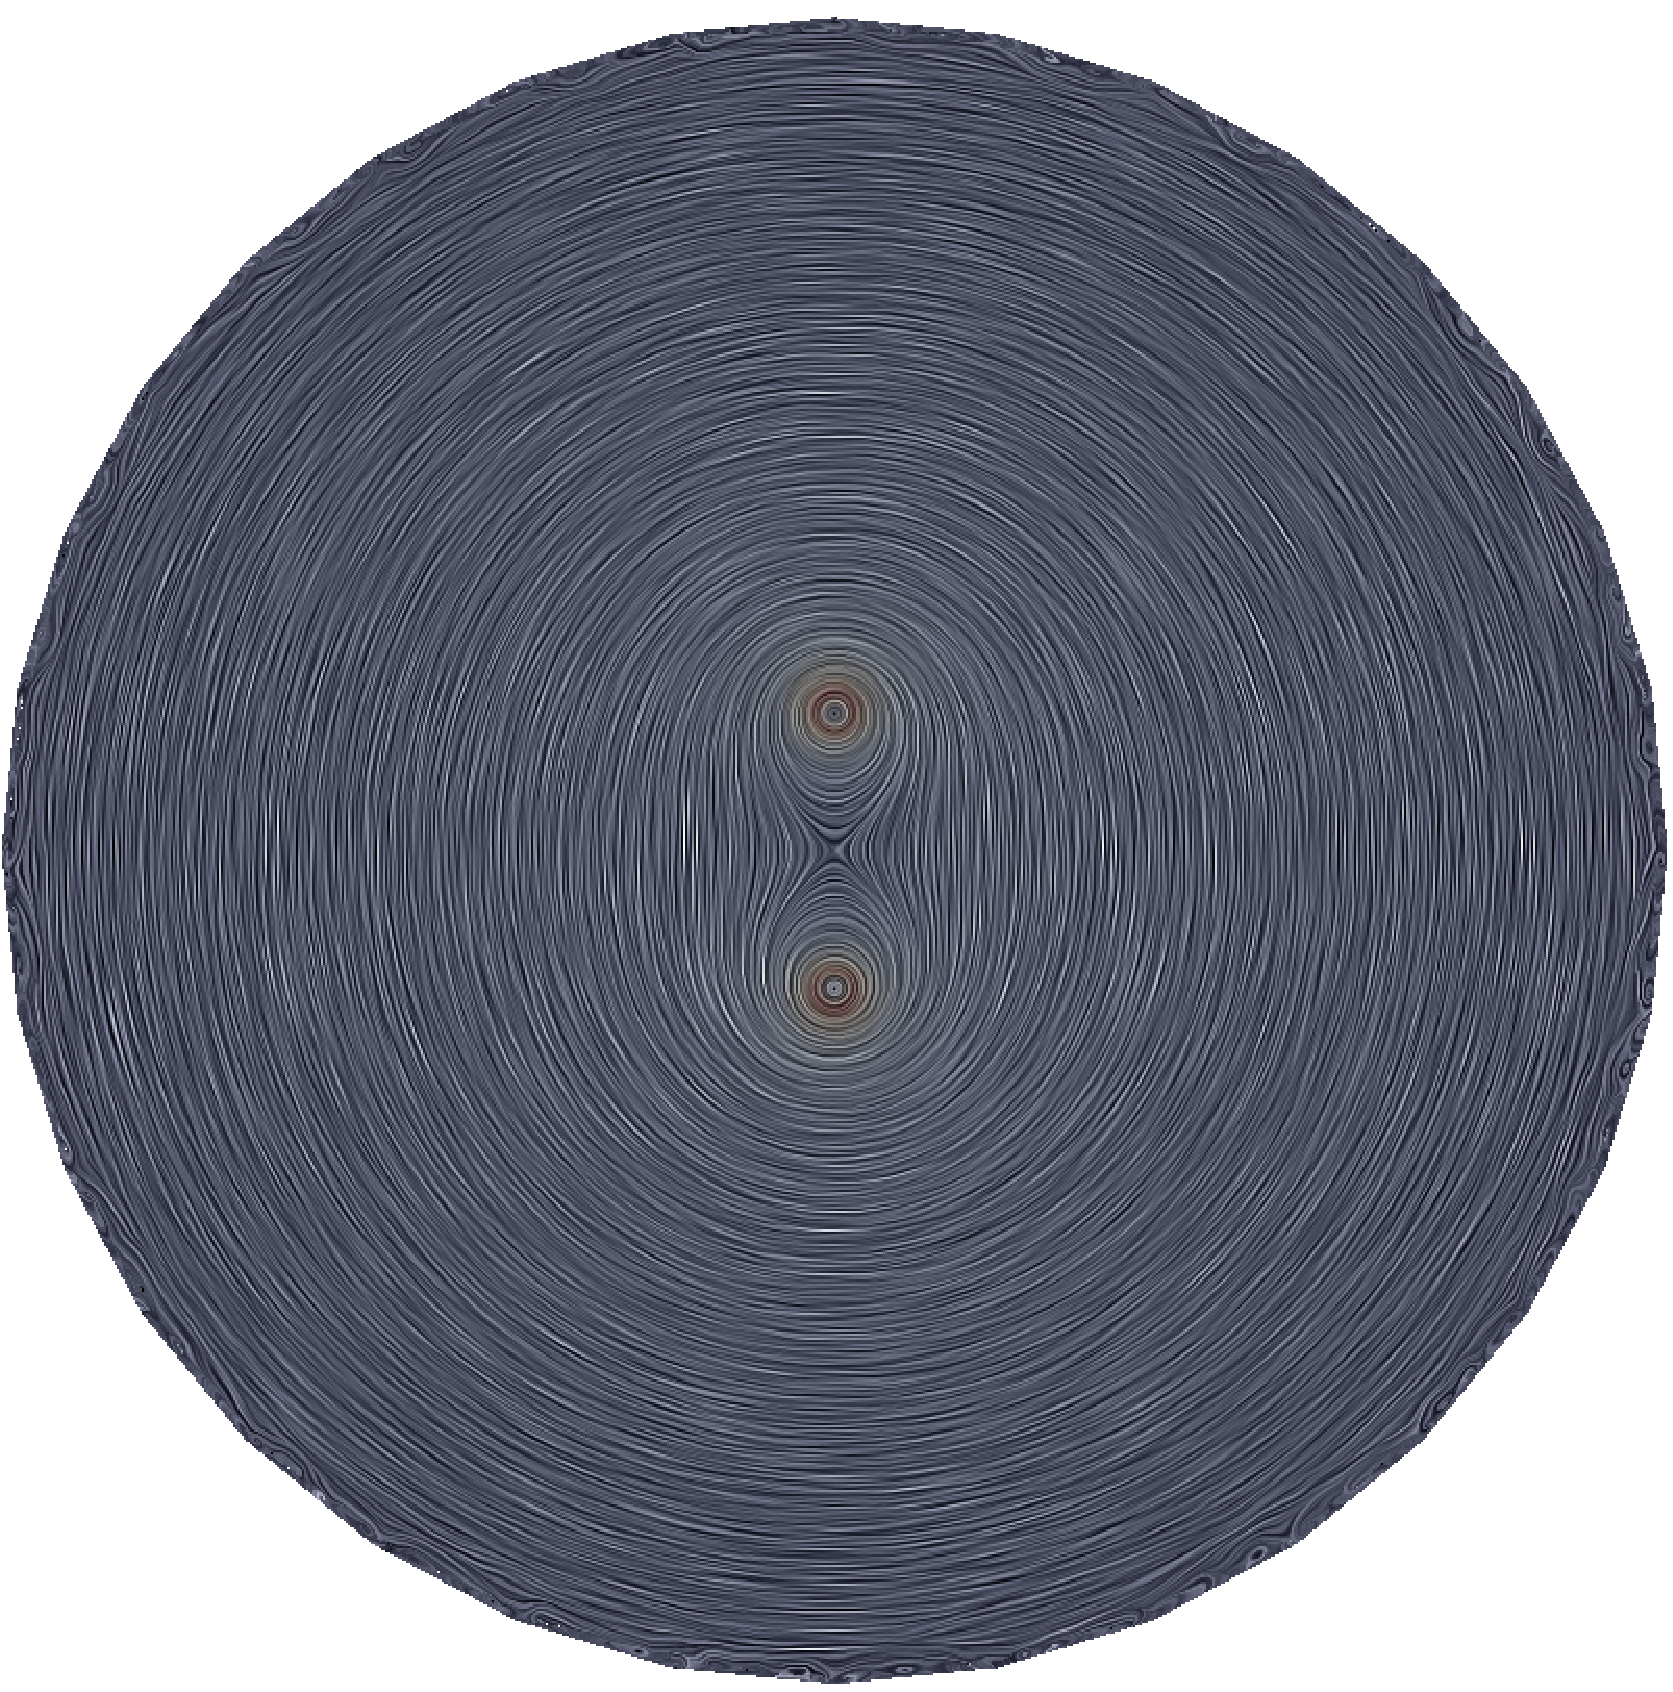
\includegraphics[width = .6\textwidth]{SR_2D_tris}
    \caption{Linee di flusso della soluzione al \textit{test case} per la BR in 2D}
    \label{fig:SR_2D_tris}
\end{figure}

In Figura \ref{fig:SR_2D} è mostrato l'andamento del campo, confrontando l'analisi senza BR  (caso \textit{a}) con quelle effettuate attivando la BR; per evidenziare la variazione di intensità di campo è mostrato il caso con ordine di decadimento $\alpha = 3$.
 
\begin{figure}
    \centering
    \subfloat[][]{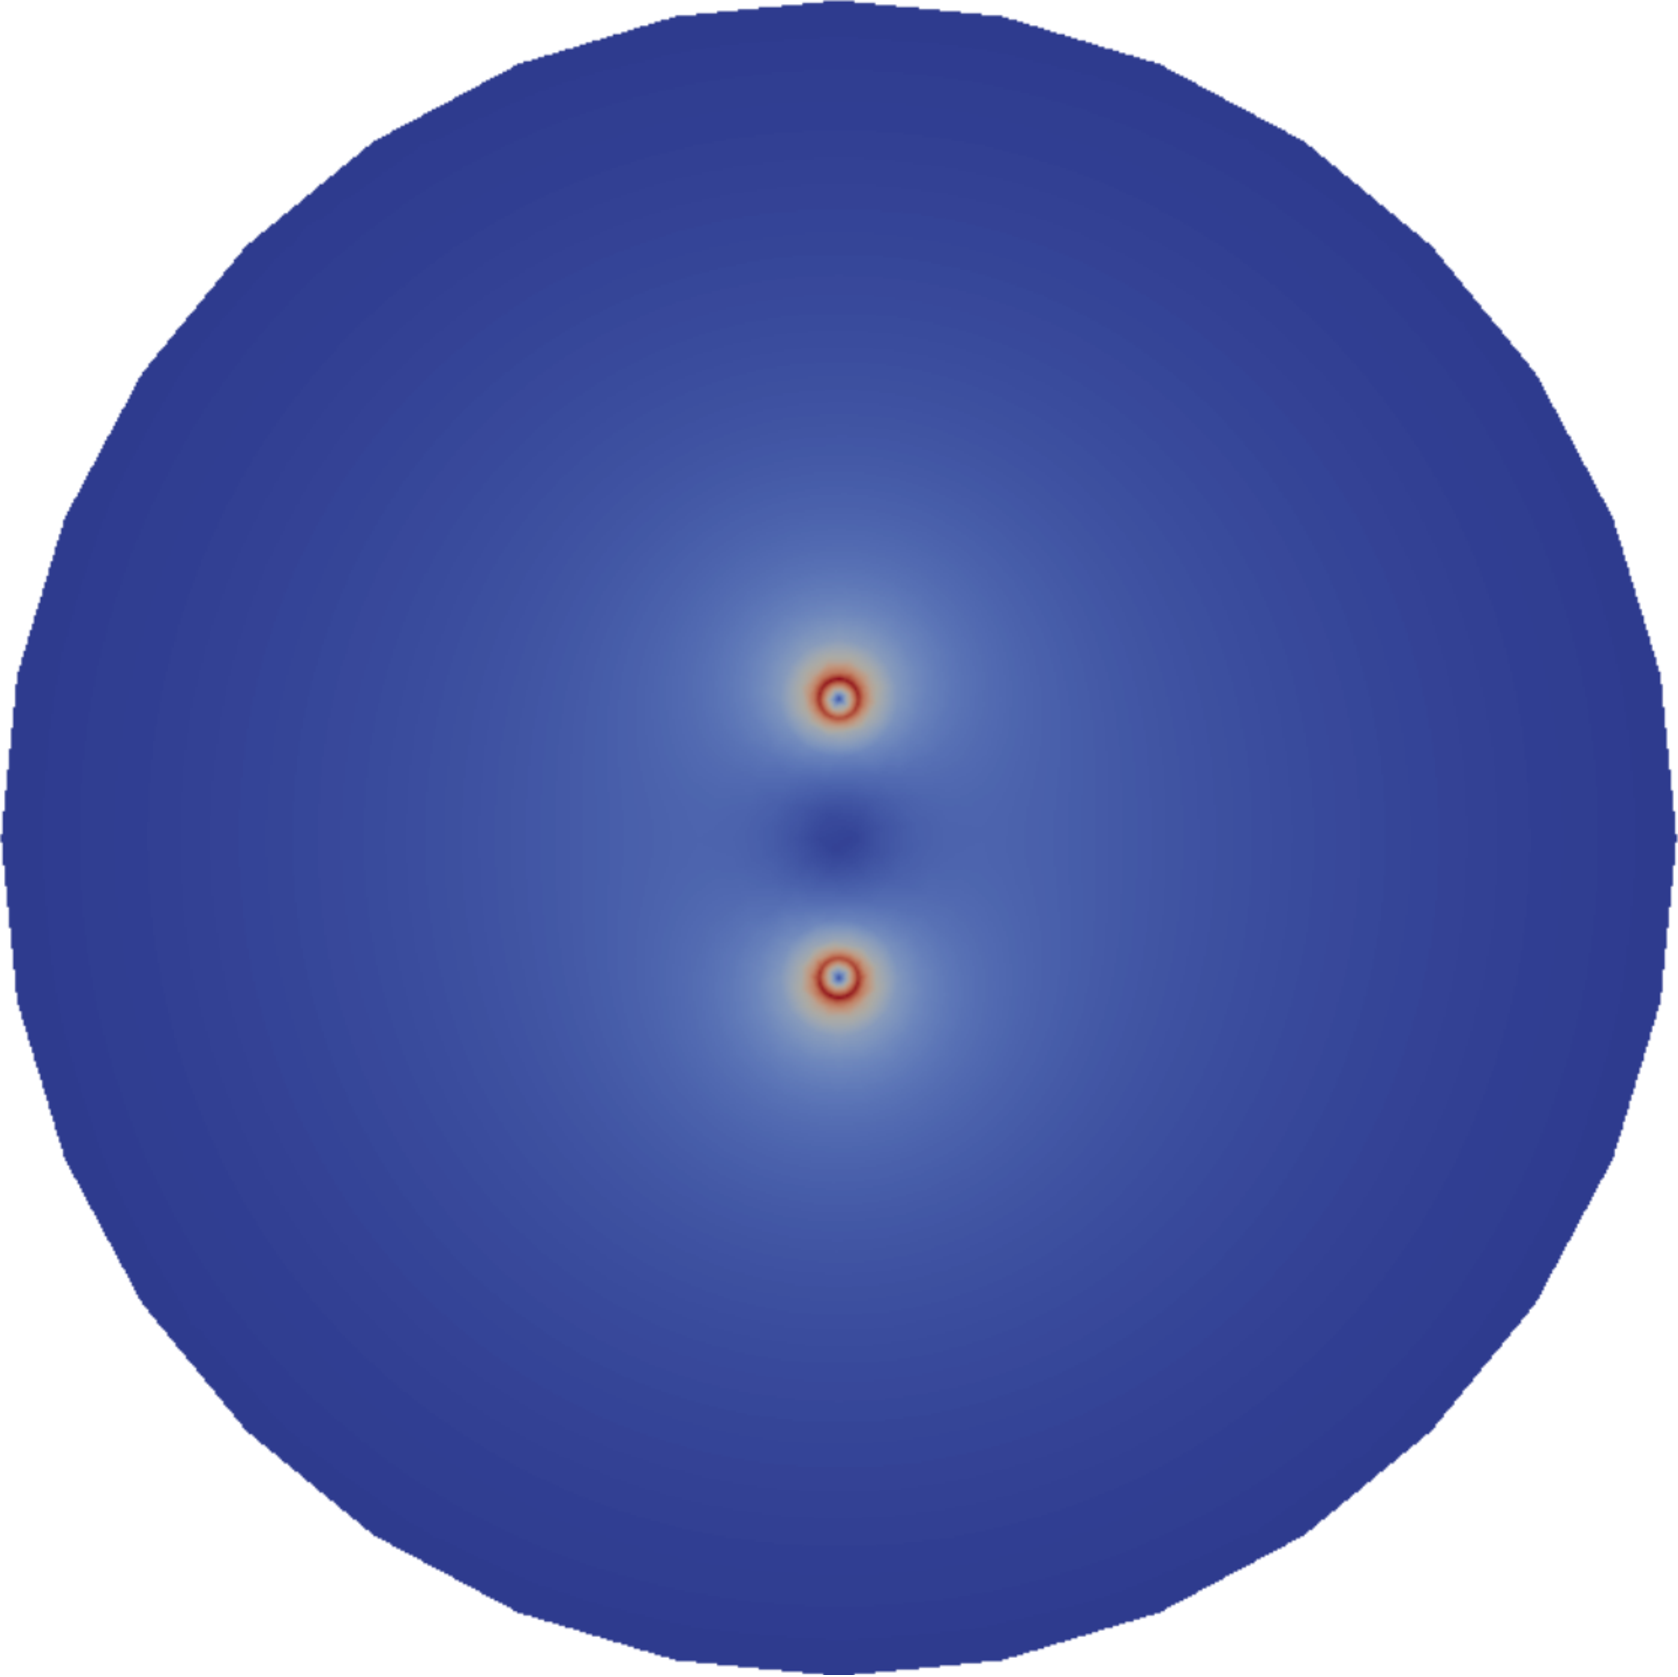
\includegraphics[width = .45\textwidth]{SR_2D_a}\label{SR_2D_a}}\quad
    \subfloat[][]{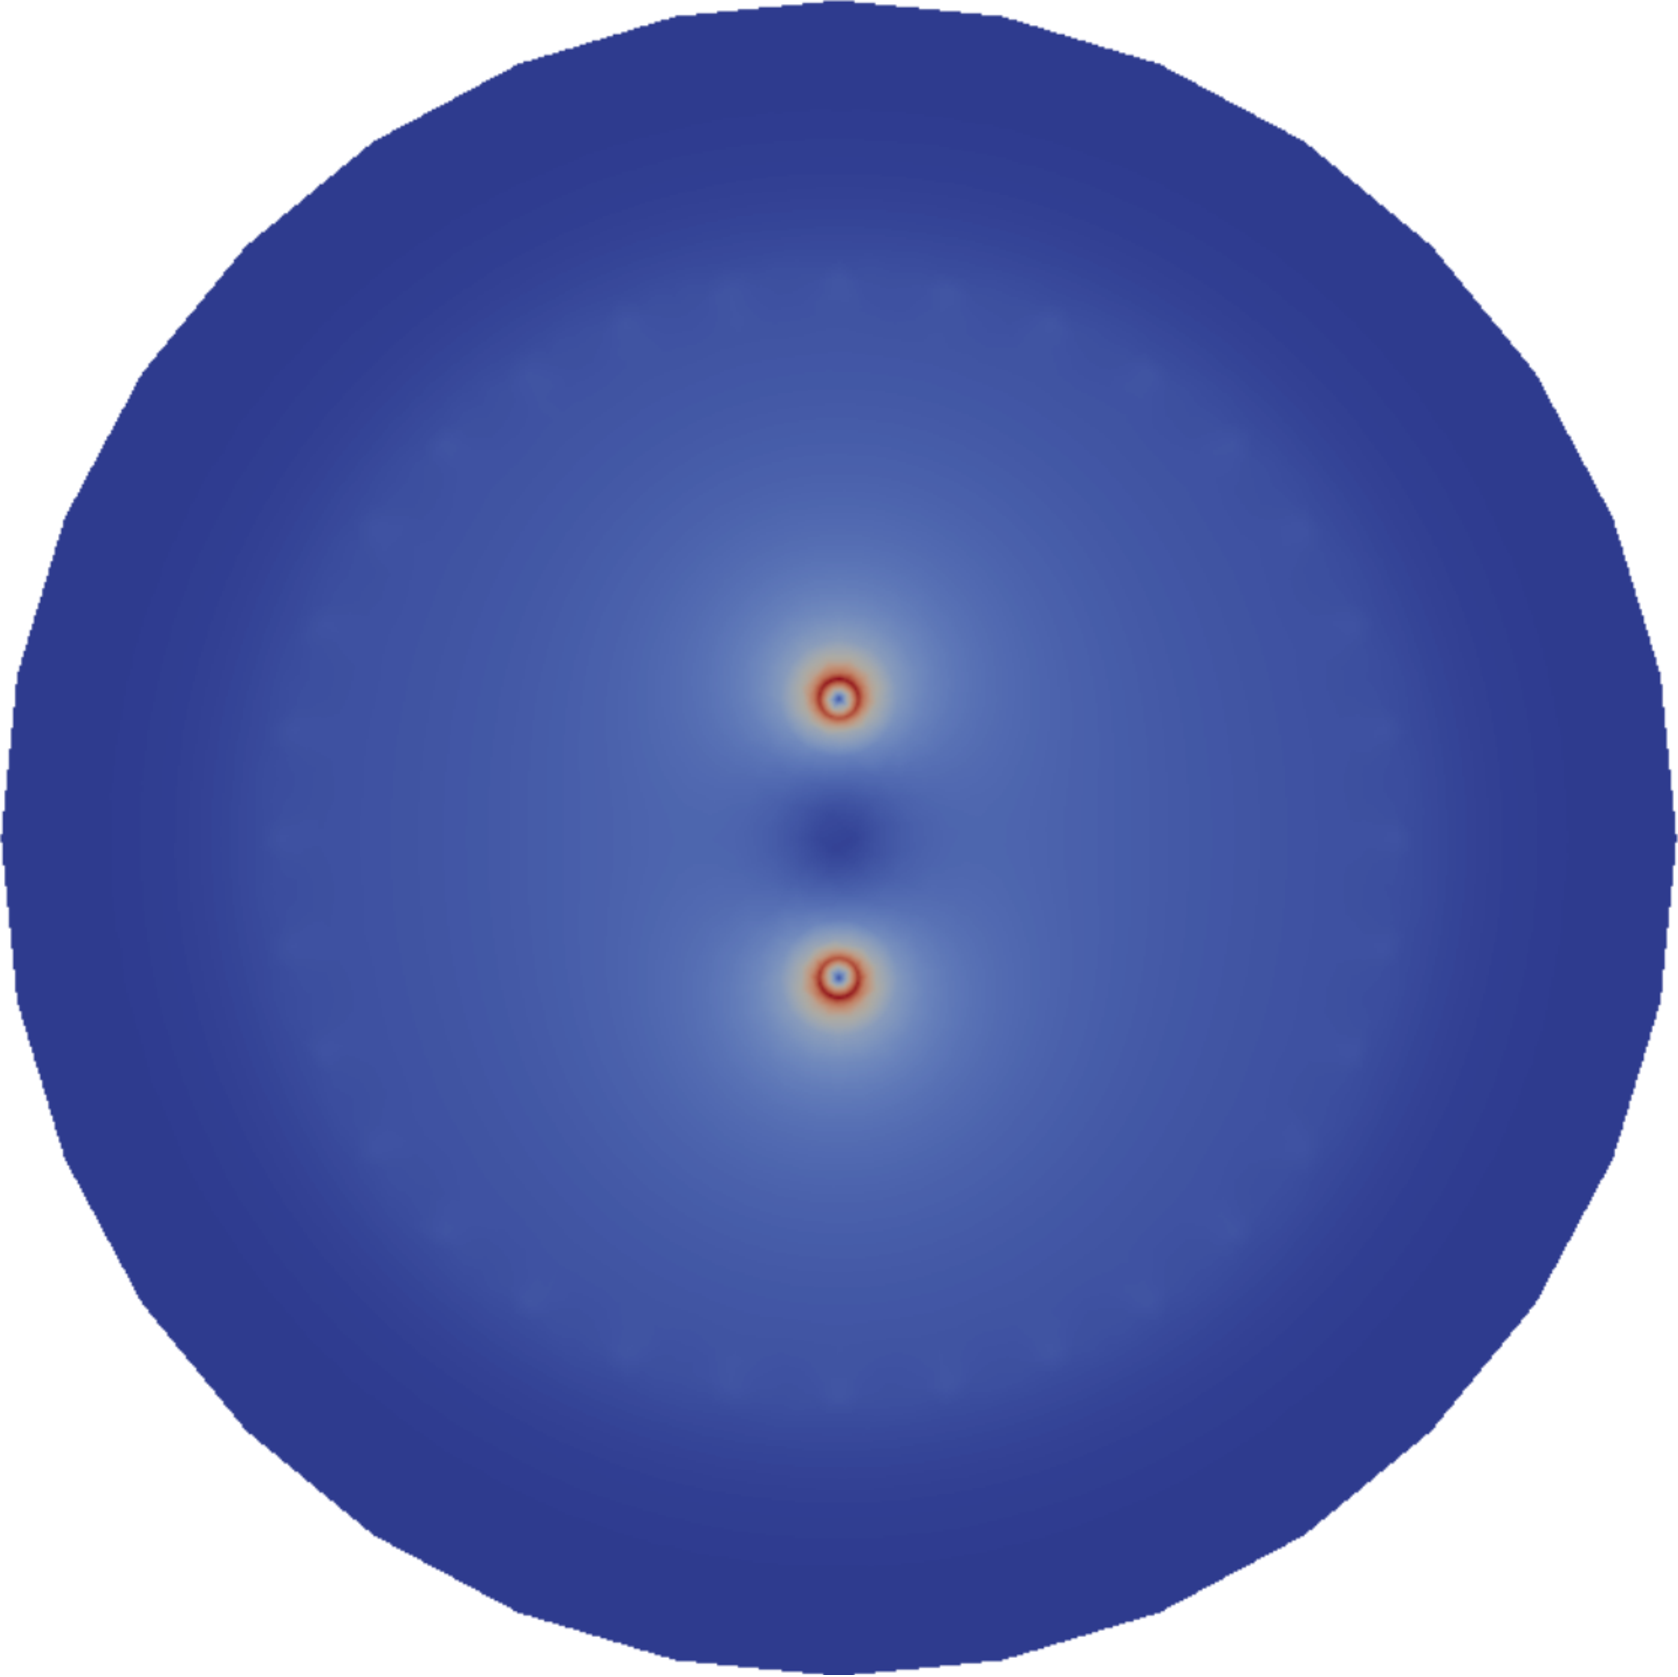
\includegraphics[width = .45\textwidth]{SR_2D_b3}\label{SR_2D_b3}}
    \caption{Confronto fra le induzioni magnetiche generate  senza e con l'attivazione della BR di ordine 3}
     \label{fig:SR_2D}
\end{figure}


Si può notare, grazie al confronto in Figura \ref{fig:SR_2D_bis} che mostra il modulo dell'induzione magnetica in funzione della distanza dal punto centrale, che il decadimento del campo magnetico viene correttamente rappresentato solo con l'attivazione del metodo.  

Si riporta che l'andamento teorico mostrato in figura è scalato di un fattore pari a 1.04 poiché, mentre nel caso ideale la corrente totale che attraversa i fili è pari a $2\pi r\T{j}$, la corrente totale nelle analisi numeriche è data da $2p\T{j}$, dove $2p$ è il perimetro effettivo della mesh che riproduce la circonferenza. Il fattore di scalatura riportato è stato ottenuto stimando il numero di lati del poligono circoscritto alla circonferenza con lato pari alla dimensione media degli elementi nella zona considerata.

Si osservi l'andamento del grafico nella zona della BR: con il primo ordine il campo assume un andamento lineare e negli altri casi l'abbattimento è più marcato. 

Si noti inoltre che i tre casi di applicazione del metodo danno curve coincidenti nella regione interna.
\begin{landscape}
\begin{figure}[htb]
   \centering
    \begin{tikzpicture}
    \begin{axis}[axis y line = left,
                 axis x line = left,
    		     xmin = 0,
    		     width = 1.5\textwidth,
    		     height = \textheight,
                 xlabel = {$r$ (m)}, 
                 ylabel = {$\T{b}$ (T)}]
    \addplot[black, samples = 200, smooth]
    file {./Immagini/Boundary/SR_2Dteorico.dat};
    \addplot[black!60!white, thick, dotted, samples = 100, smooth]
    file {./Immagini/Boundary/SR_2D_0.dat};
    \addplot[red,dashed, samples = 200, smooth]
    file {./Immagini/Boundary/SR_2D_1.dat};
    \addplot[green,dashed, samples = 100, smooth]
    file {./Immagini/Boundary/SR_2D_2.dat};
    \addplot[blue,dashed, samples = 200, smooth]
    file {./Immagini/Boundary/SR_2D_3.dat};
    \legend{$Teoric$\\$No~SST$\\$\alpha = 1$\\$\alpha = 2$\\$\alpha=3$\\}
    \draw[red,  thick] (10,0)-- (10,0.1);
    \end{axis}
    \end{tikzpicture}
    \caption{Confronto del decadimento del campo $\T{b}$ nel caso bidimensionale}
    \label{fig:SR_2D_bis}
\end{figure}
\end{landscape}




\section{Regioni conduttive in regime quasi-stazionario}

Questa sezione riassume le considerazioni fatte sull'effetto della variazione nel tempo del flusso di un campo magnetico in una regione conduttiva. La variazione di $\Phi(\T{b})$ causa la nascita di un campo elettrico all'interno del conduttore; il comportamento del materiale dipende dalla conducibilità del materiale e dalla frequenza di variazione del campo magnetico\ \citep{haus_electromagnetic_1989}.


Se la variazione di flusso è rapida (ad alta frequenza) domina il comportamento induttivo del materiale conduttore: il campo elettrico indotto provoca la nascita di correnti di spostamento $\T{j}$ che inducono a loro volta un campo magnetico. Questo si sovrappone con il campo esterno in modo da annullarlo all'interno del dominio. In questo caso si può riassumere il comportamento della regione imponendo la non-penetrazione del campo magnetico all'interno della regione conduttiva. Infatti il materiale si scherma dal campo generando delle correnti in prossimità della superficie nello stesso modo in cui si scherma dal campo elettrico generando una distribuzione di cariche superficiali. Possiamo quindi scrivere: 
\begin{equation}
\label{eq:4cond1}
\T{b}\cdot \T{n} = 0.
\end{equation}

La corrente indotta (superficiale) può essere espressa come:
\begin{equation}
\label{eq:4cond2}
\T{j_{s}} = -\T{h}\times\T{n},
\end{equation}

Se, al contrario, la variazione di flusso è lenta (a bassa frequenza) il campo elettrico indotto è troppo basso per generare un'interferenza magnetica; il conduttore è inerte e può essere trattato solamente tramite le sue proprietà magnetiche. 
In questo secondo caso, quindi, la presenza del materiale conduttore non altera le condizioni al contorno del problema magnetico. Il materiale è dominato dalle sue proprietà resistive e la corrente indotta (volumetrica) può essere calcolata a posteriori:
\begin{equation}
\label{eq:4cond3}
\T{j} = \sigma\T{e} = \sigma~\de_t\T{a}.
\end{equation}
Nella situazione intermedia la dinamica dello sviluppo delle correnti non può essere trascurata e il campo magnetico ed elettrico tornano ad essere dipendenti l'uno dall'altro, non per l'accoppiamento dinamico proprio delle equazioni di Maxwell bensì per la natura del legame costitutivo. Le analisi vengono in questi casi effettuate risolvendo equazioni di diffusione.

Poiché nel caso dell'ottica adattiva i sensori capacitivi e gli attuatori induttivi sono co-locati (e quindi molto vicini) e le frequenze di controllo sono elevate (fino a $10^5$ Hz)  è necessaria un'analisi preliminare per una stima dell'ordine di grandezza delle correnti indotte nel condensatore a causa del movimento relativo tra questo e gli elementi dell'attuatore. In questo esempio la variazione di flusso è generata dalla corrente variabile nell'induttore, ma lo stesso principio vale anche nel caso di parti in movimento relativo. In quest'ottica è stata scelta come rappresentativa la frequenza di $100$ kHz, nell'ipotesi che per frequenze maggiori l'ampiezza del movimento dello specchio sia trascurabile.

Dato che i coating metallici che compongono le armature del condensatore hanno lo spessore di pochi micron, l'analisi sarà ristretta a conduttori sottili modellabili attraverso semplici superfici conduttive.

\tikzset{
  pics/.cd,
  disc/.style = {
    code = {
      \fill [white] ellipse [x radius = 2, y radius = 2/3];
      \path [left color = black!50, right color = black!50,
        middle color = black!25] 
        (-2+.05,-1.1) arc (180:360:2-.05 and 2/3-.05*2/3) -- cycle;
      \path [top color = black!25, bottom color = white] 
        (0,.05*2/3) ellipse [x radius = 2-.05, y radius = 2/3-.05*2/3];
      \path [left color = black!25, right color = black!25,
        middle color = white] (-2,0) -- (-2,-1) arc (180:360:2 and 2/3)
        -- (2,0) arc (360:180:2 and 2/3);
      \foreach \r in {225,315}
        \foreach \i [evaluate = {\s=30;}] in {0,2,...,30}
          \fill [black, fill opacity = 1/50] 
            (0,0) -- (\r+\s-\i:2 and 2/3) -- ++(0,-1) 
            arc (\r+\s-\i:\r-\s+\i:2 and 2/3) -- ++(0,1) -- cycle;
      \foreach \r in {45,135}
        \foreach \i [evaluate = {\s=30;}] in {0,2,...,30}
          \fill [black, fill opacity = 1/50] 
            (0,0) -- (\r+\s-\i:2 and 2/3) 
            arc (\r+\s-\i:\r-\s+\i:2 and 2/3)  -- cycle;
    }
  },
  disc2/.style = {
    code = {
      \fill [white] ellipse [x radius = 2, y radius = 2/3];
      \path [top color = black!25, bottom color = white] 
        (0,.05*2/3) ellipse [x radius = 2-.05, y radius = 2/3-.05*2/3];
      \path [left color = black!25, right color = black!25,
        middle color = white] (-2,0) -- (-2,-.01) arc (180:360:2 and 2/3)
        -- (2,0) arc (360:180:2 and 2/3);
      \foreach \r in {225,315}
        \foreach \i [evaluate = {\s=30;}] in {0,2,...,30}
          \fill [black, fill opacity = 1/50] 
            (0,0) -- (\r+\s-\i:2 and 2/3) -- ++(0,-.01)
            arc (\r+\s-\i:\r-\s+\i:2 and 2/3) -- ++(0,.01)-- cycle;
      \foreach \r in {45,135}
        \foreach \i [evaluate = {\s=30;}] in {0,2,...,30}
          \fill [black, fill opacity = 1/50] 
            (0,0) -- (\r+\s-\i:2 and 2/3) 
            arc (\r+\s-\i:\r-\s+\i:2 and 2/3)  -- cycle;
    }
  }
}
\begin{SCfigure}[1.5][htb]
\centering
\caption{Esempio di analisi di diffusione: piastra metallica posta a breve distanza da un solenoide}
\label{fig:4cond_ind_example}
\tdplotsetmaincoords{55}{45}
\resizebox{.3\textwidth}{!}{
\begin{tikzpicture}
\path (0,0) pic {disc} (0,0.4) pic {disc2};
\end{tikzpicture}}
\end{SCfigure}


Si prenda in considerazione il sistema mostrato in Figura \ref{fig:4cond_ind_example} composto da una piastra metallica sottile posta su un induttore solenoidale.

Si supponga per semplicità che il solenoide generi un campo $\T{h}$ armonico con periodo $T$ che in prossimità della piastra sia costante e normale alla superficie. Considerando una circonferenza di raggio $r<R$ interna al disco si ha allora:
\begin{equation}
\label{eq:4es1}
2\pi r e = \mu \pi r^2 \de_t h,
\end{equation}
da cui
\begin{equation}
\label{eq:4es2}
e = \mu \frac{r}{2} \de_t h.
\end{equation}

Se la piastra possiede uno spessore $t$, scriviamo la corrente superficiale equivalente:

\begin{equation}
\label{eq:4es3}
j_s = \sigma e t = \mu \sigma \frac{r}{2} t \de_t h.
\end{equation}

\begin{table}
\centering
\caption{Dati ipotizzzati per la stima dell'entità del campo indotto su un sensore capacitivo} \label{tab:4daties}
\begin{tabular}{lc}
\toprule
Tipo sensore & Coating aureo\\
\midrule
Spessore & $1~\mu\text{m}$\\
Raggio & $10^-2$ m\\
Conduttività & $4.2553191~10^7 \frac{1}{\Omega\text{m}}$\\
Frequenza di controllo & $10^5 \text{Hz}$\\
\bottomrule
\end{tabular}
\end{table}
Si può ora stimare l'entità del campo magnetico indotto, approssimando l'integrale della corrente superficiale (che cresce linearmente con $r$) con il prodotto del raggio medio $R/2$ e della corrente corrispondente $j_s(R/2)$:
\begin{align}
\label{eq:4es4}
2\pi \frac{R}{2} h_{ind} &= i_{enc} = \int_0^R j_s(\chi) d\chi \approx \frac{R}{2} j_s (\frac{R}{2})\\
\label{eq:4es5}
h_{ind} &\approx\frac{\frac{R}{2} j_s (\frac{R}{2})}{2\pi \frac{R}{2}} = \frac{j_s(\frac{R}{2})}{2 \pi}.
\end{align}

Ne consegue un campo indotto medio pari a:
\begin{equation}
\label{eq:4es6}
h_{ind} \approx \mu \frac{ \sigma R t}{8\pi} \de_t h,
\end{equation}
da cui si ottiene un rapporto fra il campo generato dal solenoide $h$ e il campo indotto $h_{ind}$:
\begin{equation}
\label{eq:4es6bis}
\frac{h_{ind}}{h} \approx \mu \frac{ \sigma R t}{8\pi} \frac{\de_t h}{h} = \mu \frac{ \sigma R t}{8\pi} \omega = \mu \frac{ \sigma R t}{4T}.
\end{equation}

Si applichi la formula appena ottenuta supponendo dimensioni e frequenze compatibili con i sistemi applicati per l'ottica adattiva (Tabella \ref{tab:4daties}). Si ha:
\begin{equation}
\label{eq:4es7}
\frac{h_{ind}}{h}\approx 0.02
\end{equation}

Tale valore, ottenuto con ipotesi conservative (campo magnetico perpendicolare alla superficie conduttiva, stime pessimistiche dell'ordine di grandezza) suggerisce un comportamento del conduttore dominato dalle sue caratteristiche resistive. Questo legittima l'ipotesi dell'indipendenza del campo magnetico relativo agli attuatori dalla presenza dei sensori capacitivi. 

% !TEX encoding = UTF-8 Unicode
% !TEX TS-program = pdflatex
% !TEX root = ../Tesi.tex



%************************************************
\myChapter{Problemi al contorno}
%************************************************
\label{cap:bvp}

In questo capitolo viene presentata la formulazione di un problema al contorno consistente (\textit{Boundary Value Problem, BVP})  per le equazioni differenziali derivate dal problema elettromagnetico presentato nel Capitolo \ref{cap:maxwell}. 


I potenziali introdotti in Sezione \ref{subsec:1potenziale} ben si prestano alla scrittura in forma debole delle equazioni di Maxwell. In questo modo, con riferimento al problema originario, le due equazioni \eqref{eq:2max1} e \eqref{eq:2max4} saranno soddisfatte in forma forte.

Verrà inoltre da qui in avanti abbandonato il regime dinamico completo per focalizzare l'attenzione sui regimi ridotti adeguati alle analisi effettuate in questo lavoro.

Infine, verranno utilizzati unicamente legami costitutivi isotropi, così da ridurre i tensori $\TT{\varepsilon}$ e $\TT{\mu}$ alle quantità scalari $\varepsilon$ e $\mu$.

Come si è potuto osservare nel capitolo precedente, nelle due formulazioni ridotte \textit{MQS} e stazionaria le equazioni sono disaccoppiate nei due campi $\left\{\T{a},\phi\right\}$:
\begin{equation}
\left\{
\label{eq:3potqss}
\begin{aligned}
\lap\left({\phi}\right) &= -\varepsilon^{-1} \rho\\
-\lap\left(\T{a}\right) &= \mu\T{j}+\rot\left(\T{b_r}\right).
\end{aligned}
\right.
\end{equation}
I due regimi si differenziano nel recupero dei campi $\left\{\T{e},\T{b}\right\}$:

\begin{equation}
\label{eq:2recuperoqss}
\begin{aligned}
&\text{MQS}\\
&\left\{
\begin{aligned}
\T{b}&=\rot \left(\T{a}\right)\\
\T{e} &= -\grad\left(\phi\right) -\partial_t \T{a}
\end{aligned}
\right.
\end{aligned}
\qquad
\begin{aligned}
&\text{STAZIONARIO}\\
&\left\{
\begin{aligned}
\T{b}&=\rot \left(\T{a}\right)\\
\T{e} &= -\grad\left(\phi\right)
\end{aligned}
\right.
\end{aligned}
\end{equation}

Durante la presentazione dei potenziali si è evidenziato l'utilizzo per i regimi ridotti della condizione di gabbia di Gauss \eqref{eq:2gaussgauge}. L'imposizione di tale condizione comporta l'interscambiabilità dei seguenti termini:
\begin{equation}
\label{eq:3rotrotlap}
\rot\left[\rot\left(\T{a}\right)\right] = -\lap\left(\T{a}\right)
\end{equation}
all'interno della seconda delle equazioni \eqref{eq:3potqss}. 

Verranno ora introdotti gli ambienti naturali per lo sviluppo della forma debole, per poi analizzare in dettaglio le formulazioni per il problema magnetico ed elettrico.

\section{Spazi funzionali}

Si definisca lo spazio
\begin{equation}
\label{eq:3L2}
L_2\left(\TTTT{D}\right) := \left\{ u | \int_{\TTTT{D}} u^2 dv < \infty\right\},
\end{equation}
che fornito del prodotto scalare
\begin{equation}
\label{eq:3scaL2}
\left(u,v\right)= \int_{\TTTT{D}} u\,v\, dv,
\end{equation}
costituisce uno spazio di Hilbert.

Si richiamano ora le definizioni degli \textit{operatori differenziali generalizzati}:
\begin{enumerate}


\item $D_u = u'$ è detta \textit{derivata generalizzata} di $u \in L_2\left(\TTTT{D}\right)$ se 
\begin{equation}
\label{eq:3gen_der}
\int_{\TTTT{D}}D_u w\, dv = - \int_{\TTTT{D}}u \,w' \, dv \qquad \forall w \in C_0^\infty\left(\bar{\TTTT{D}}\right),
\end{equation}
dove $\bar{\TTTT{D}}$ è un sottoinsieme compatto di $\TTTT{D}$ e costituisce il supporto delle \textit{test function} $w$. 
\item $\T{g}=\grad\left(u\right)$ è detto \textit{gradiente generalizzato} di $u \in  L_2\left(\TTTT{D}\right)$ se
\begin{equation}
\label{eq:3gen_grad}
\int_{\TTTT{D}}\T{g}\cdot \T{w}\, dv = - \int_{\TTTT{D}}u \,\dive\left(\T{w}\right) \, dv \qquad \forall \T{w} \in \left(C_0^\infty\left(\bar{\TTTT{D}}\right)\right)^3.
\end{equation}
\item $\T{r}=\rot\left(\T{u}\right)$ è detto \textit{rotore generalizzato} di $\T{u} \in  \left(L_2\left(\TTTT{D}\right)\right)^3$ se
\begin{equation}
\label{eq:3gen_rot}
\int_{\TTTT{D}}\T{r}\cdot \T{w}\, dv =  \int_{\TTTT{D}}\T{u}\cdot \rot\left(\T{w}\right) \, dv \qquad \forall \T{w} \in \left(C_0^\infty\left(\bar{\TTTT{D}}\right)\right)^3.
\end{equation}
\item $d = \dive\left(\T{u}\right)$ è detta \textit{divergenza generalizzata} di $\T{u} \in  \left(L_2\left(\TTTT{D}\right)\right)^3$ se
\begin{equation}
\label{eq:3gen_div}
\int_{\TTTT{D}}d\, w\, dv =  \int_{\TTTT{D}}\T{u}\cdot \grad\left(w\right) \, dv \qquad \forall w \in C_0^\infty\left(\bar{\TTTT{D}}\right).
\end{equation}
\end{enumerate}

Si possono ora definire i seguenti spazi funzionali:
\begin{eqnarray}
\label{eq:3h1}
H^1\left(\TTTT{D}\right) &:=&\left\{ w \in L_2\left(\TTTT{D}\right) | \grad\left( w\right) \in \left(L_2\left(\TTTT{D}\right)\right)^3\right\},\\
\label{eq:3hcurl}
H\left(\rot,\TTTT{D}\right) &:=&\left\{ \T{w} \in \left(L_2\left(\TTTT{D}\right)\right)^3 | \rot\left( \T{w}\right) \in \left(L_2\left(\TTTT{D}\right)\right)^3\right\},\\
\label{eq:3hdiv}
H\left(\dive,\TTTT{D}\right) &:=&\left\{ \T{w} \in \left(L_2\left(\TTTT{D}\right)\right)^3 | \dive\left( \T{w}\right) \in L_2\left(\TTTT{D}\right)\right\}.
\end{eqnarray}

A questi vengono associati i seguenti prodotti scalari:
\begin{eqnarray}
\label{eq:3scah1}
\left(u,v\right)_1 &=& \int_{\TTTT{D}} \grad\left(u\right)\cdot\grad\left(v\right)dv+\left(u,v\right),\\
\label{eq:3scahcurl}
\left(\T{u},\T{v}\right)_{\rot} &=& \int_{\TTTT{D}}\rot\left(\T{u}\right)\cdot\rot\left(\T{v}\right)dv+\left(\T{u},\T{v}\right),\\
\label{eq:3scahdiv}
\left(\T{u},\T{v}\right)_{\dive} &=& \int_{\TTTT{D}}\dive\left(\T{u}\right)\dive\left(\T{v}\right)dv+\left(\T{u},\T{v}\right).
\end{eqnarray}

Gli spazi sopra definiti, se forniti delle norme associate ai rispettivi prodotti scalari,  sono spazi di Hilbert.

\section{Forma debole per il problema magnetico}

Si consideri l'equazione:
\begin{equation}
\rot\left[\rot\left(\T{a}\right)\right] = \mu\T{j}+\rot\left(\T{b_r}\right),
\label{eq:3strong1}
\end{equation}
alla quale vengono associate le condizioni di interfaccia derivanti dalle equazioni \eqref{eq:4interface_b3} e \eqref{eq:4interface_h}:
\begin{equation}
\left\{
\begin{aligned}
&\Bigl\langle \rot\left(\T{a}\right)\times \T{n}\Bigr\rangle = -\mu\T{j_s} \\
&\Bigl\langle \rot\left(\T{a}\right)\cdot \T{n}\Bigr\rangle = 0.
\end{aligned}
\right.
\label{eq:3interface_a}
\end{equation}

Si noti che la seconda delle due condizioni al contorno è equivalente a
\begin{equation}
\label{eq:3interface_a2}
\Bigl\langle \T{a}\times \T{n}\Bigr\rangle = 0.
\end{equation}
\\
Sia ora $\T{a}\in H\left(\rot,\TTTT{D}\right)$; per ogni dominio $\TTTT{D}$ si integri l'equazione \eqref{eq:3strong1} e la prima delle condizioni al contorno \eqref{eq:3interface_a} e le si moltiplichino per una \textit{test function} vettoriale $\T{w} \in H\left(\rot,\TTTT{D}\right)$:
\begin{align}
\label{eq:3weak1}
&\int_{\TTTT{D}}\T{w} \cdot \rot\left[\rot\left(\T{a}\right)\right] dv+\int_{\partial\TTTT{D}}\T{w}\cdot \left[\rot\left(\T{a}\right)\times\T{n}\right]ds= \nonumber\\
&=\int_{\TTTT{D}}\T{w}\cdot\left[\mu\T{j}+rot\left(\T{b_r}\right)\right]dv+\int_{\partial\TTTT{D}}\T{w}\cdot \mu\T{j_s} ds.
\end{align}

Si sfrutti ora la relazione vettoriale
\begin{equation}
\dive\left[\T{u}\times \rot\left(\T{v}\right)\right] = \rot\left(\T{u}\right)\cdot \rot\left(\T{v}\right)-\T{u}\cdot \rot\left[rot\left(\T{v}\right)\right]
\label{eq:3vectrel}
\end{equation}
per riscrivere l'equazione \eqref{eq:3weak1}:
\begin{align}
\label{eq:3weak2}
&\int_{\TTTT{D}}\rot\left(\T{w}\right)\cdot \rot\left(\T{a}\right) dv-\int_{\TTTT{D}} \dive\left[\T{w}\times \rot\left(\T{a}\right)\right] dv + \nonumber\\
&+\int_{\partial\TTTT{D}}\T{w}\cdot \left[\rot\left(\T{a}\right)\times\T{n}\right]ds= \nonumber\\
&=\int_{\TTTT{D}}\T{w}\cdot\left[\mu\T{j}+\rot\left(\T{b_r}\right)\right]dv+\int_{\partial\TTTT{D}}\T{w}\cdot \mu\T{j_s} ds.
\end{align}

Si applichi ora il teorema di Gauss al termine di divergenza:
\begin{align}
\label{eq:3weak3}
&\int_{\TTTT{D}}\rot\left(\T{w}\right)\cdot \rot\left(\T{a}\right) dv-\int_{\partial\TTTT{D}} \left[\T{w}\times \rot\left(\T{a}\right)\right]\cdot \T{n} ds + \nonumber\\
&+\int_{\partial\TTTT{D}}\T{w}\cdot \left[\rot\left(\T{a}\right)\times\T{n}\right]ds= \nonumber\\
&=\int_{\TTTT{D}}\T{w}\cdot\left[\mu\T{j}+\rot\left(\T{b_r}\right)\right]dv+\int_{\partial\TTTT{D}}\T{w}\cdot \mu\T{j_s} ds.
\end{align}

Si può dimostrare che i due termini in $\partial\TTTT{D}$ nel primo membro dell'Eq. \eqref{eq:3weak2} sono uguali citando l'identità vettoriale:
\begin{equation}
\label{eq:3vectidentity}
\T{p} \cdot (\T{q} \times \T{r}) = \T{q} \cdot (\T{r} \times \T{p}) = \T{r} \cdot (\T{p} \times \T{q}).
\end{equation}

Si ottiene pertanto:
$\forall \,\T{w} \in H(\rot,D)$:
\begin{align}
\label{eq:3weak4}
&\int_{\TTTT{D}}\rot\left(\T{w}\right)\cdot \rot\left(\T{a}\right) dv
= \nonumber\\
&=\int_{\TTTT{D}}\T{w}\cdot\left[\mu\T{j}+\rot\left(\T{b_r}\right]\right)dv+\int_{\partial\TTTT{D}}\T{w}\cdot \mu\T{j_s} ds.
\end{align}

A questa forma debole deve essere incorporata la condizione di gabbia sul potenziale \eqref{eq:2gaussgauge} unitamente alla seconda delle condizioni al contorno \eqref{eq:3interface_a}; si introducano una \textit{test function}  $\psi$ e la corrispondente \textit{trial function} $\chi$ appartenenti allo spazio funzionale $H^1\left(\TTTT{D}\right)$. Si ha, sfruttando la definizione di divergenza generalizzata \eqref{eq:3gen_div}, l'ortogonalità del potenziale vettoriale rispetto ai gradienti:
\begin{equation}
\label{eq:3weakgauge}
\int_{\TTTT{D}} \T{a} \cdot \grad\left(\psi\right) dv = 0 \qquad \forall \psi \in H^1\left(\TTTT{D}\right).
\end{equation}

 Si ottiene così la cosiddetta \textit{formulazione magnetostatica mista}, per la cui soluzione esistenza e unicità possono essere dimostrate mediante il Teorema di \textit{Brezzi} e il Teorema di \textit{Lax-Milgram}, omessi in questa trattazione \citep{zaglmayr_high_2006}.
 
\begin{itemize}
\item $\forall \T{w} \in H(\rot,\TTTT{D})$:
\begin{align}
\label{eq:3weak3_a}
\int_{\TTTT{D}_i}\rot\left(\T{w}\right)\cdot \rot\left(\T{a}\right) dv +\int_{\TTTT{D}_i} \T{w} \cdot \grad \left(\chi\right) dv
= \nonumber\\
=\int_{\TTTT{D}_i}\T{w}\cdot\left[\mu\T{j}+\rot\left(\T{b_r}\right]\right)dv+\int_{\partial\TTTT{D}_i}\T{w}\cdot \mu\T{j_s} ds;
\end{align}
\item $\forall \psi \in H^1(\TTTT{D})$:
\begin{align}
\label{eq:3weak3_b}
\int_{\TTTT{D}_i}\grad \left(\psi\right) \cdot \T{a}  dv = 0.
\end{align}
\end{itemize}

Questa formulazione, per quanto efficacie ed utilizzabile, comporta la necessità dell'introduzione del campo scalare $\chi$ aggiuntivo. Oltre all'ovvio aumento delle dimensioni del sistema, questa formulazione può portare a cattivo condizionamento dello stesso e ad una lenta convergenza nell'utilizzo di solutori lineari. Viene qui  pertanto introdotta una formulazione mista \textit{regolarizzata} tramite il parametro scalare $k$

$\forall \T{w} \in H(\rot,\TTTT{D})$: 
\begin{align}
\label{eq:3weak5}
\int_{\TTTT{D}_i}\rot\left(\T{w}\right)\cdot \rot\left(\T{a}\right) dv +k\int_{\TTTT{D}_i} \T{w} \cdot \T{a} dv
= \nonumber\\
=\int_{\TTTT{D}_i}\T{w}\cdot\left[\mu\T{j}+\rot\left(\T{b_r}\right)\right]dv+\int_{\partial\TTTT{D}_i}\T{w}\cdot \mu\T{j_s} ds.
\end{align}

Può essere dimostrato che tale formulazione converge ad una soluzione unica $\T{a_k}$ e che tale soluzione coincide con quella del problema non regolarizzato per $k\rightarrow 0$. 

\'E utile esprimere il parametro $k$ in relazione a $\mu_0$. In relazione al condizionamento del problema i seguenti valori sono stati sperimentati con successo: 

\begin{equation}
\label{eq:3 regpar}
k = c \mu_0 , \qquad 1<= c <=1000
\end{equation}
\section{Forma debole per il problema elettrico}

In analogia con quanto appena trattato per il potenziale magnetico, si imposta qui una struttura per la costruzione del problema in forma debole per il problema elettrico.

 In Sezione \ref{subsec:1potenziale} si è visto come il campo elettrico possa essere scomposto nell'ambito del regime \textit{MQS} in una parte solenoidale $\T{e_f}$ e in una irrotazionale $\T{e_c}$. Confrontando le equazioni \eqref{eq:2e_coulomb}, \eqref{eq:2e_faraday} e \eqref{eq:2max12s} si può osservare come nel regime stazionario (elettrostatica) la parte solenoidale sia identicamente nulla. 

La determinazione di $\T{e_f}$ deriva dall'analisi magnetica trattata nella sezione precedente. 

Per ottenere $\T{e_c}$ occorre cercare una forma debole della prima delle equazioni \eqref{eq:3potqss}
unitamente alle condizioni di interfaccia:

\begin{equation}
\left\{
\begin{aligned}
&\Bigl\langle \grad\left(\phi\right)\times \T{n}\Bigr\rangle = 0 \\
&\Bigl\langle \grad\left(\phi\right)\cdot \T{n}\Bigr\rangle = \rho_s.
\end{aligned}
\right.
\label{eq:3interface2_a}
\end{equation}

Sia ora $\phi \in H^1\left(\TTTT{D}\right)$; integrando l'Eq. \eqref{eq:3potqss} e la seconda delle condizioni al contorno \eqref{eq:3interface2_a} e moltiplicandole per una \textit{test function} $w \in H^1\left(\TTTT{D}\right)$ si ha :

\begin{align}
\label{eq:3weak_e1}
&-\int_{\TTTT{D}}w \, \lap\left(\phi\right) dv+\int_{\partial\TTTT{D}}w \, \grad\left(\phi\right)\cdot \T{n}ds= \nonumber\\
&=\varepsilon^{-1}\int_{\TTTT{D}}w\,\rho dv+\varepsilon^{-1}\int_{\partial\TTTT{D}}w\, \rho_s ds
\end{align}

\begin{eqnarray}
\label{eq:3weak_e2}
-\int_{\TTTT{D}}\dive\left[w \, \grad\left(\phi\right)\right]dv+ \int_{\TTTT{D}}\grad\left(w\right)\cdot \grad\left(\phi\right)dv+\\ +\int_{\partial\TTTT{D}}w \, \grad\left(\phi\right)\cdot \T{n}ds= \nonumber\\
=\varepsilon^{-1}\int_{\TTTT{D}}w\,\rho dv+\varepsilon^{-1}\int_{\partial\TTTT{D}}w\, \rho_s ds.
\end{eqnarray}

Utilizzando il teorema di Gauss per il primo termine, si ha:
\begin{eqnarray}
\label{eq:3weak_e3}
-\int_{\partial\TTTT{D}}w \, \grad\left(\phi\right)ds +\int_{\TTTT{D}}\grad\left(w\right)\cdot \grad\left(\phi\right)dv+\nonumber\\ +\int_{\partial\TTTT{D}}w \, \grad\left(\phi\right)\cdot \T{n}ds= \nonumber\\
=\varepsilon^{-1}\int_{\TTTT{D}}w\,\rho dv+\varepsilon^{-1}\int_{\partial\TTTT{D}}w\, \rho_s ds,
\end{eqnarray}
da cui
\begin{align}
\label{eq:3weak_e4}
&\int_{\TTTT{D}}\grad\left(w\right)\cdot \grad\left(\phi\right)dv = \nonumber\\
&=\varepsilon^{-1}\int_{\TTTT{D}}w\,\rho dv+\varepsilon^{-1}\int_{\partial\TTTT{D}}w\, \rho_s ds.
\end{align}

Come per il problema magnetico, per $w$ e $\phi \in H^1\left(\TTTT{D}\right)$ è dimostrabile l'esistenza e unicità della soluzione. \'E inoltre implicitamente soddisfatta la prima delle \eqref{eq:3interface2_a} \citep{zaglmayr_high_2006}.

\section{Conclusioni}

Nelle precedenti sezioni sono state presentate le forme deboli utilizzate nel corso di questo lavoro. 

L'esistenza e unicità delle soluzioni dei precedenti problemi sono garantite previa corretta impostazione del problema: il codice a elementi finiti deve pertanto utilizzare elementi conformi agli spazi funzionali presenti. I classici elementi finiti "lagrangiani" con  incognite nodali sono conformi agli spazi $H^1(\TTTT{D})$ e $H^(div, \TTTT{D})$, ma per la conformità ad $H(rot,\TTTT{D})$ si è reso necessario l'utilizzo di una diversa classe di elementi: gli elementi di spigolo (\textit{edge elements}). La principale proprietà di questi elementi è la possibilità di ottenere la formulazione di un problema la cui soluzione è richiesta conforme ad $H(rot,\TTTT{D})$ in termini di gradi di libertà esplicitamente indipendenti \citep{bossavit_computational_1998}. Fra gli elementi appartenenti a questa classe si è scelto di utilizzare gli elementi di Nédélec \citep{nedelec_acoustic_2001}. L'utilizzo di tali elementi, rispetto ad elementi nodali comporta grossi vantaggi per i problemi in forma debole presentati:
\begin{itemize}
\item Maggiore precisione a parità di griglia di calcolo
\item Miglior condizionamento della matrice assemblata
\end{itemize}

Ne risulta una robusta convergenza della soluzione con metodi iterativi.


In Tabella \ref{tab:tabella_campi} sono riassunti i risultati ottenuti in uno schema che mostra, per ciascun campo incognito, lo spazio funzionale adeguato e la classe di elementi utilizzata in questa analisi.

\begin{table}[h]
\centering
\caption{Elenco degli spazi funzionali appropriati e degli elementi utilizzati per i campi in gioco}
\footnotesize
\label{tab:tabella_campi}
\begin{tabular}{lcccc}
\toprule
Campo & Simbolo &Tipologia & Spazio funzionale & Elemento\\
\midrule
Campo elettrico & $\T{e}$ & vettoriale & $H(rot,\TTTT{D})$ & Nèdèlec\\
Campo magnetico & $\T{h}$ & vettoriale & $H(rot,\TTTT{D})$ & Nèdèlec\\
Induzione elettrica & $\T{d}$ & vettoriale & $H(div,\TTTT{D})$ & Lagrange\\
Induzione magnetica & $\T{b}$ & vettoriale & $H(div,\TTTT{D})$ & Lagrange\\
Potenziale elettrico & $\phi$ & vettoriale & $H^1(\TTTT{D})$ & Lagrange\\
Potenziale magnetico & $\T{a}$ & vettoriale & $H(rot,\TTTT{D})$ & Nèdèlec\\
\bottomrule
\end{tabular}
\end{table}

\section{Scaling}
I calcoli sono stati eseguiti in alcuni casi in parallelo sfruttando diverse \textit{CPU} per l'assemblaggio e la risoluzione del sistema lineare. Si riportano in questa sezione i risultati dei test di scalabilità effettuati per la valutazione delle prestazioni del solutore in funzione del numero di \textit{core} utilizzati.

\subsection{Strong scaling}
Per \textit{strong scaling} si intende l'analisi del tempo di calcolo necessario al programma per risolvere un determinato sistema al variare del numero di core. In Figura \ref{fig:strongscaling} è riportato il grafico delle prestazioni ottenute su un problema di esempio di calcolo del campo magnetico attorno a due magneti permanenti. Il grafico mostra soltanto i tempi di calcolo in parallelo, che nel programma sono preceduti dalle operazioni di \textit{preprocessing} eseguite in seriale con un processore. In Tabella \ref{tab:strongscaling} sono elencati i dati del modello e i tempi ottenuti.

\begin{table}[p]
\centering
\begin{minipage}{0.45\textwidth}
\centering
\tiny
\begin{tikzpicture}
    \begin{axis}[axis y line = left,
                 axis x line = left,
    		     width = \textwidth,
    		     height = .3\textheight,
                 xlabel = {cores}, 
                 ylabel = {tempo (s)}]
                 \addplot[mark = *]
    file {./Immagini/BVP/strongscaling.dat};
    \end{axis}
\end{tikzpicture}
\captionof{figure}{\textit{Strong scaling}}
\label{fig:strongscaling}
\end{minipage}
\begin{minipage}{0.45\textwidth}
\centering
\tiny
\caption{Dati del modello e tempi ottenuti per l'analisi di \textit{strong scaling}}
\label{tab:strongscaling}
\begin{tabular}{lc}
\toprule
Dati del modello&\\
\midrule
N. di vertici & 97609\\
N. di celle & 576435\\
\midrule
Tempi di calcolo seriale\\
\midrule
Meshing (gmsh) & 60.9 s\\
Conversione mesh & 28.9 s\\
Preprocessing & 8.7 s\\
\midrule
Sistemi risolti&\\
Sistema 1 & $675552\times675552$\\
Sistema 2 & $2319483\times2319483$\\
Sistema 3 & $878481\times878481$\\
\midrule
Tempi di calcolo\\
\midrule
1 \textit{core} & 231.3 s\\
2 \textit{core} & 215.7 s\\
4 \textit{core} & 153.3 s\\
6 \textit{core} & 140.8 s\\
\bottomrule
\end{tabular}
\end{minipage}
\end{table}


\subsection{Weak scaling}
Per \textit{weak scaling} si intende l'analisi delle prestazioni misurando il tempo di calcolo al variare del numero di core assegnando a ciascun processore la stessa mole di calcolo (quindi raddoppiando le dimensioni del sistema quando raddoppia il numero di core). In Figura \ref{fig:weakscaling} è riportato il grafico delle prestazioni ottenute. In Tabella \ref{tab:weakscaling} sono elencati i dati del modello e i tempi ottenuti.
\begin{table}[p]
\centering
\begin{minipage}{0.45\textwidth}
\centering
\tiny
\begin{tikzpicture}
    \begin{axis}[axis y line = left,
                 axis x line = left,
    		     width = \textwidth,
    		     height = .3\textheight,
                 xlabel = {cores}, 
                 ylabel = {tempo (s)}]
                 \addplot[mark = *]
    file {./Immagini/BVP/weakscaling.dat};
    \end{axis}
\end{tikzpicture}
\captionof{figure}{\textit{Weak scaling}}
\label{fig:weakscaling}

\end{minipage}
\begin{minipage}{0.45\textwidth}
\centering
\tiny
\begin{tabular}{lc}
\toprule
1 Processore&\\
\midrule
N. di vertici & 5243\\
N. di celle & 30713\\
Sistemi risolti&\\
Sistema 1 & $36066\times36066$\\
Sistema 2 & $123927\times123927$\\
Sistema 3 & $47187\times47187$\\
Tempo di calcolo & 10.0 s\\
\midrule
2 Processori&\\
\midrule
N. di vertici & 9686\\
N. di celle & 56970\\
Sistema 1 & $66827\times66827$\\
Sistema 2 & $229539\times229539$\\
Sistema 3 & $87174\times87174$\\
Tempo di calcolo & 13.6862208843 s\\
\midrule
4 Processori&\\
\midrule
N. di vertici & 18757\\
N. di celle & 110294\\
Sistemi risolti&\\
Sistema 1 & $129434\times129434$\\
Sistema 2 & $444573\times444573$\\
Sistema 3 & $444573\times444573$\\
Tempo di calcolo & 25.1 s\\

\bottomrule
\end{tabular}
\caption{Dati del modello e tempi ottenuti per l'analisi di \textit{weak scaling}}
\footnotesize
\label{tab:weakscaling}
\end{minipage}
\end{table}

I risultati ottenuti non sono soddisfacenti; si ritiene possa essere opportuno estendere il lavoro sviluppando un'interfaccia per il solutore \textit{AMS} dell libreria \textit{hypre}, che rappresenta il primo solutore scalabile per problemi elettromagnetici \citep{AMS_hypre}.
% !TEX encoding = UTF-8 Unicode
% !TEX TS-program = pdflatex
% !TEX root = ../Tesi.tex



%************************************************
\myChapter{Elaborazione dei risultati}
%************************************************
\label{cap:output}
In questo capitolo verrà posta attenzione sull'estrazione di risultati utili dalle analisi numeriche svolte:
\begin{itemize}
\item Forze e coppie
\item Induttanze
\item Capacità
\end{itemize}
\section{Forze e coppie}
Il calcolo di forze e coppie elettromagnetiche è di primaria importanza nell'ambito dell'analisi di dispositivi elettromeccanici. 

Tuttavia, come si vedrà in questo capitolo, è tutt'altro che agevole laddove non si debbano calcolare forze su cariche note, siano esse ferme o in movimento. 
Un esempio è il magnete permanente: come si è visto nel capitolo \ref{cap:maxwell}, l'orientamento delle orbite elettroniche all'interno dei domini è un fenomeno stocastico rappresentato tramite un modello macroscopicamente equivalente. Tale modello non è adatto al calcolo diretto delle forze agenti sulle cariche \textit{reali} in movimento all'interno del mezzo. Si rende pertanto necessario l'utilizzo di specifiche tecniche per il calcolo delle forze scambiate fra magneti permanenti.

Iniziamo quindi introducendo le forze agenti in un volume in cui vi sia una densità di carica $\rho$ in moto con velocità $\T{v}$:

\begin{align}
\label{eq:5coulombf}
&\text{Forza di \textit{Coulomb}} &\T{f_c}=\rho \T{e}  \\
\label{eq:5lorentzf}
&\text{Forza di \textit{Lorentz}}&\T{f_l}=\rho \T{v}\times \T{b} .
\end{align}

Si ottiene quindi la forza totale esercitata dai due campi:
\begin{equation}
\label{eq:5ftot1}
\T{f}=\rho \left(\T{e}+\T{v}\times \T{b}\right).
\end{equation}

Nel caso in cui vi siano soltanto cariche in quiete e cariche in movimento modellabili come correnti stazionarie la forza totale può essere espressa come:
\begin{equation}
\label{eq:5ftot2}
\T{f}=\rho\T{e} +\T{j}\times \T{b}.
\end{equation}

Laddove le forze non possano essere espresse tramite le espressioni di Lorentz e Coulomb, vengono adottati metodi di origine diversa, che si differenziano per precisione, difficoltà di implementazione, praticità di utilizzo.
\subsection{Metodo delle cariche magnetiche equivalenti}
 Questo metodo consiste nella modellazione della magnetizzazione residua $\T{m_r}$ tramite una distribuzione di cariche virtuali nel volume e sulla superficie del magnete:
\begin{align}
\label{eq:5cariche_eq1a}
&\rho =-\dive \left(\T{m_r}\right) \qquad  &\text{in $V$,}\\
\label{eq:5cariche_eq1b}
&\rho_s =\T{m_r}\cdot \T{n} \qquad &\text{in $\de V$.}
\end{align}
Sotto l'azione di un campo magnetico esterno si ottiene quindi una forza \citep{furlani_permanent_2001}:
\begin{equation}
\label{eq:5sourcef}
\T{F} = \int_V \rho\T{b} dv+\int_{\de V} \rho_s \T{b} ds. 
\end{equation}
Si può osservare come nel caso di magnetizzazione costante nei diversi domini le forze siano superficiali.
Nel caso in cui vi siano domini con diverse magnetizzazioni adiacenti, considerando l'orientazione delle rispettive normali con riferimento alla Figura \ref{fig:5.1}, si ha per i termini di superficie:
\begin{align}
\label{eq:5sourcef2}
\T{f_{s1}}&=\left(\T{n_1}\cdot\T{m_{r1}}\right)\bar{\T{b}}\nonumber\\
\T{f_{s2}}&=\left(\T{n_2}\cdot\T{m_{r2}}\right)\bar{\T{b}}\nonumber\\
\T{f_{s}}&=\langle\T{n}\cdot\T{m_{r}}\rangle\bar{\T{b}},
\end{align}
dove $\bar{\T{b}}$ è la media dell'induzione magnetica a cavallo dell'interfaccia ($\bar{\T{b}}=\left(\T{b_1}+\T{b_2}\right)/2$).
\begin{SCfigure}
\caption{Domini per il calcolo di forze superficiali tramite cariche e correnti equivalenti}
\label{fig:5.1}
\begin{tikzpicture}
\draw[black] (0,0) circle (3);
\draw[black] (0,3) arc (90:270:3);
\draw[->] (0,0) -- (1,0);
\fill[black!10!white, opacity = .8] (0,0) ellipse (.6 and 3);
\draw[dashed] (0,3) arc (90:270:.6 and 3);
\draw (0,3) arc (450:270:.6 and 3);
\draw[->] (2.2,-0.9) -- (2.4,.1);
\draw[->] (-2.2,-.5) -- (-2.4,0.5);
\shade[ball color=black!10!white,opacity=0.20] (0,0) circle (3);

\draw[->] (0,0) -- (-1,0);
\draw (-2,-.9) node {$\T{m_{r1}}$}; %label
\draw (1.95,-1.1) node {$\T{m_{r2}}$}; %label
\draw (1.15,0.15) node {$\T{n_1}$}; %label
\draw (-1.15,0.15) node {$\T{n_2}$}; %label
\draw (1.15,2.15) node {$V_2$}; %label
\draw (-1.15,2.15) node {$V_1$}; %label
\end{tikzpicture}
\end{SCfigure}
\subsection{Metodo delle correnti magnetiche equivalenti} Come nel metodo precedente si cerca un'espressione della magnetizzazione residua; in questo caso viene adottato un modello a correnti:
\begin{align}
\label{eq:5correnti_eq1a}
&\T{j} =\rot\left(\T{m_r}\right) \qquad  &\text{in $V$,}\\
\label{eq:5correnti_eq1b}
&\T{j_s} =\T{m_r}\times \T{n} \qquad &\text{in $\de V$.}
\end{align}
Riscriviamo la forza di Lorentz:
\begin{equation}
\label{eq:5currentf}
\T{F} = \int_V \T{j}\times\T{b} dv+\int_{\de V} \T{j_s} \times \T{b} ds. 
\end{equation}
Anche in questo caso otteniamo i termini di superficie nel caso di due domini adiacenti:
\begin{align}
\label{eq:5currentf2}
\T{f_{s}}&=\langle\T{m_{r}}\times\T{n}\rangle\times\bar{\T{b}}.
\end{align}
Si sottolinea qui che i due metodi appena presentati forniscono solo una rappresentazione globale equivalente ai fini del calcolo del campo magnetico al di fuori del dominio dei magneti permanenti; permettono pertanto soltanto il calcolo delle forze risultanti (e delle relative coppie) e non delle forze distribuite (locali) \citep{de_medeiros_about_1999}.
\subsection{Tensore di Maxwell} Questo strumento molto versatile permette di calcolare forze di origine elettrica e magnetica in un contesto assolutamente generale, indipendente dal regime utilizzato e dalla natura delle forze che originano i campi.

Si inizi esplicitando i termini $\rho$ e $\T{j}$ dall'equazione \eqref{eq:5ftot2} in funzione del campo elettrico $\T{e}$ e dell'induzione magnetica $\T{b}$:
\begin{align}
\label{eq:5maxf1}
\T{f}&=\dive\left(\T{d}\right) \T{e} +\left[\rot\left(\T{h}\right)-\de_t \T{d}\right]\times \T{b}\nonumber\\
&=\varepsilon\dive\left(\T{e}\right) \T{e} +\left[\mu^{-1}\rot\left(\T{b}\right)-\varepsilon\de_t \T{e}\right]\times \T{b}.
\end{align}

Si utilizzi la relazione:
\begin{equation}
\label{eq:5vectid}
\de_t\left(\T{e}\times\T{b}\right) = \de_t \T{e}\times \T{b} + \T{e}\times\de_t\T{b}
\end{equation}
per riscrivere l'ultimo termine dell'equazione \eqref{eq:5maxf1}:
\begin{align}
\label{eq:5maxf2}
\T{f}=\varepsilon\dive\left(\T{e}\right) \T{e} &+\mu^{-1}\rot\left(\T{b}\right)\times \T{b}+\nonumber\\
&-\varepsilon \left[\de_t\left(\T{e}\times\T{b}\right)-\T{e}\times\de_t\T{b}\right]
\end{align}
e, per la legge di Faraday,
\begin{align}
\label{eq:5maxf3}
\T{f}=\varepsilon\dive\left(\T{e}\right) \T{e} &+\mu^{-1}\rot\left(\T{b}\right)\times \T{b}+\nonumber\\
&-\varepsilon \left[\de_t\left(\T{e}\times\T{b}\right)+\T{e}\times\rot\left(\T{e}\right)\right].
\end{align}
Per simmetria, si aggiunga il termine (identicamente nullo) $\mu^{-1} \dive\left(\T{b}\right)\T{b}$:
\begin{align}
\label{eq:5maxf4}
\T{f}=\varepsilon\dive\left(\T{e}\right) \T{e} +\mu^{-1} \dive\left(\T{b}\right)\T{b}+\nonumber\\
-\mu^{-1}\T{b}\times\rot\left(\T{b}\right) -\varepsilon\T{e}\times\rot\left(\T{e}\right)+\nonumber\\
-\varepsilon\de_t\left(\T{e}\times\T{b}\right).
\end{align}
Si utilizzi ora l'identità vettoriale
\begin{equation}
\label{eq:5vectid2}
\grad\left(\T{v}\cdot\T{v}\right) = 2 \T{v}\times\rot\left(\T{v}\right)+2\grad\left(\T{v}\right)\T{v}
\end{equation}
così da ottenere
\begin{align}
\label{eq:5maxf5}
\T{f}=\varepsilon \left[ \dive \left( \T{e} \right) \T{e} + \grad \left( \T{e} \right) \T{e} \right] +\nonumber\\
+\mu^{-1} \left[\dive\left(\T{b}\right)\T{b}+\grad\left(\T{b}\right)\T{b}\right] +\nonumber\\
-\frac{1}{2} \grad\left[\varepsilon\left(\T{e}\cdot\T{e}\right)+
\mu^{-1}\left(\T{b}\cdot\T{b}\right) \right] +\nonumber\\
-\varepsilon\de_t\left(\T{e}\times\T{b}\right).
\end{align}
In questo modo la forza per unità di volume può essere espressa in funzione del \textit{vettore di Poynting} $\T{s}$ e del \textit{tensore di Maxwell} $\TT{T}$ \citep{griffiths_introduction_2013}:
\begin{equation}
\label{eq:5poyntandmax}
\left\{
\begin{aligned}
\T{s} &= \mu^{-1} \T{e}\times\T{b}\\
\TT{T} &= \varepsilon\left[\T{e}\otimes\T{e} -\frac{1}{2}\left(\T{e}\cdot\T{e}\right)\TT{I}\right] +
\mu^{-1}\left[\T{b}\otimes\T{b} -\frac{1}{2}\left(\T{b}\cdot\T{b}\right)\TT{I}\right]
\end{aligned}
\right.
\end{equation}

\begin{equation}
\label{eq:5poyntandmax2}
\T{f} = \dive\left(\TT{T}\right) -\varepsilon\mu^{-1} \de_t\T{s},
\end{equation}

dove $\TT{I}$ è il tensore identità di secondo ordine. 

Nell'approccio ai regimi ridotti si elide il contributo dovuto al tensore di Poynting. In questo modo la forza elettromagnetica dipende solamente dal tensore di Maxwell.

Applicando ora il teorema di Gauss all'equazione \eqref{eq:5poyntandmax2} si ottiene un'espressione diretta della forza elettromagnetica totale in un volume $V$ tramite il calcolo del flusso del tensore di Maxwell:

\begin{equation}
\label{eq:5maxf6}
\int_V\T{f} = \int_V\dive\left(\TT{T}\right)dv = \int_{\de V}\TT{T}\cdot \T{n}ds.
\end{equation}

Questo importante risultato permette di ottenere forze (e coppie) totali agenti su un corpo scegliendo un'opportuna superficie che circondi il corpo. \'E importante sottolineare come il risultato numerico non sia indipendente dalla scelta della superficie; in particolare si osserva che se la superficie coincide (o è sufficientemente vicina) alla superficie fisica di un corpo non si ottengono risultati attendibili. Tale comportamento è particolarmente evidente nelle analisi 3D. \'E opportuno scegliere la superficie dove la distribuzione di forza (attesa) è più regolare possibile. 
Vengono qui elencati accorgimenti e limiti del metodo, ottenuti con prove numeriche.
\begin{enumerate}
\item La superficie \textit{non può} intersecare il confine tra due domini con proprietà elettromagnetiche diverse. Come visto nei capitoli precedenti, la condizione di interfaccia porta discontinuità nei campi.
\item  La superficie deve attraversare solamente materiali diamagnetici o ferromagnetici (tipicamente si sceglie l'aria che circonda i corpi).
\item La superficie deve essere sufficientemente lontana dalle sorgenti di campo.
\item Le superfici possono avere spigoli vivi, ma quanto più le superfici sono regolari tanto più il calcolo sarà accurato. Forme sferiche o calotte emisferiche portano in genere a buoni risultati.
\item Si può abbinare il questo metodo con la tecnica delle trasformazioni al contorno (vedi sezione \ref{sec:dominiaperti}): in questo caso, se si sceglie come volume racchiuso dalla superficie di Maxwell l'intero volume di calcolo, compresa la regione della \textit{shell boundary region}, il flusso del tensore all'infinito (la superficie esterna) è intrinsecamente nullo; le forze saranno così ottenute unicamente dal flusso che attraversa la superficie di interfaccia tra le due regioni (indicata in rosso in Figura \ref{fig:5.2}).
\end{enumerate}

\begin{figure}
\centering
\caption{Suddivisione delle regioni per un utilizzo abbinato del tensore di Maxwell e di una trasformazione al contorno}
\label{fig:5.2}
\begin{tikzpicture}
\draw[black] (0,0) circle (4.5);
\fill[red!10!white, opacity = .8] (0,0) ellipse (4.5 and .9);
\draw[black] (0,0) ellipse (4.5 and .9);
\shade[ball color=black!10!white,opacity=0.20] (0,0) circle (4.5);
\draw[black,dashed] (0,0) circle (3);
\draw[black,dashed] (0,0) ellipse (3 and .6);
\shade[ball color=black!10!white,opacity=0.20] (0,0) circle (3);
\shade[ball color=black!50!white,opacity=1] (0,1.5) circle (.3);
\shade[ball color=black!50!white,opacity=1] (0,-1.5) circle (.3);
\draw[->] (4,4) -- (3.2,2);
\draw (4,4.3) node {Shell boundary region}; %label
\draw[->] (4,-3.5) -- (3.3,0);
\draw (4.,-3.8) node {Interfaccia}; %label
\end{tikzpicture}
\end{figure}

\subsection{Principio dei Lavori Virtuali (PLV)}
Sotto questo nome rientrano i metodi che ottengono la forza a partire dall'energia del campo elettromagnetico. Tali metodi competono per generalità e applicabilità con il tensore di Maxwell.

Ci limiteremo al calcolo delle forze dovute al campo magnetico in quanto, come per i metodi precedenti, il grosso vantaggio è insito nel calcolo di forze dovute a magnetizzazioni permanenti.

Le forze di origine elettromagnetica sono ottenute grazie alla derivata dell'energia magnetica rispetto ad uno spostamento arbitrario.

Per questo il PLV può essere sfruttato in  due modi:
\begin{itemize}
\item Per ottenere forze e coppie globali esprimendo la variazione di energia magnetica rispetto al movimento (o alla rotazione) di un corpo secondo un grado di libertà rigido;
\item Per ottenere la distribuzione locale di forze magnetiche esprimendo la variazione di energia magnetica rispetto al movimento di ogni singolo grado di libertà degli elementi. 
\end{itemize}

Per le analisi successive è stato implementato unicamente il primo dei due metodi perché di più immediata realizzazione.

L'energia magnetica per unità di volume è esprimibile come:
\begin{equation}
w = \int \T{h}\cdot d\T{b}. 
\label{eq:5en1}
\end{equation}

Utilizzando il legame costitutivo \eqref{eq:2costmag} si ottiene:
\begin{equation}
w = \int \mu^{-1}\left(\T{b}-\T{b_r}\right) \cdot d\T{b}. 
\label{eq:5en2}
\end{equation}

In base alla scelta degli estremi di integrazione si ottengono varie espressioni dell'energia che, vista la linearità dell'espressione rispetto a $\T{b}$, differiscono per una costante \citep{henrotte_computation_2004}:
\begin{align}
\label{eq:5en3}
w &= \mu^{-1}\frac{\T{b}\cdot\T{b}}{2}\\
\label{eq:5en4}
w &= \mu^{-1}\left(\frac{\T{b}\cdot\T{b}}{2}-\T{b}\cdot\T{b_r}\right)\\
\label{eq:5en5}
w &= \mu^{-1}\frac{\left(\T{b}-\T{b_r}\right)\cdot\left(\T{b}-\T{b_r}\right)}{2}
\end{align}

Allo stesso modo l'energia complementare, per definizione
\begin{equation}
w' = \int \T{b}\cdot d\T{h} = \int \left(\mu\T{h}+\T{b_r}\right) \cdot d\T{b}
\label{eq:5enc1}
\end{equation}
assume (utilizzando il medesimo legame costitutivo) le diverse forme:
\begin{align}
\label{eq:5enc3}
w' &= \mu\frac{\T{h}\cdot\T{h}}{2}\\
\label{eq:5enc4}
w' &= \mu\frac{\T{h}\cdot\T{h}}{2}+\T{h}\cdot\T{b_r}\\
\label{eq:5enc5}
w' &= \mu\frac{\left(\T{h}+\T{m}\right)\cdot\left(\T{h}+\T{m}\right)}{2}
\end{align}
Poiché forze e coppie sono ottenute mediante variazioni di queste quantità, nel caso di legame costitutivo lineare tutte le espressioni sopra elencate sono equivalenti.\\

La forza meccanica di origine magnetica può essere calcolata integrando tali espressioni in tutto il dominio di analisi e calcolando la derivata (ad esempio tramite schemi alle differenze finite) rispetto allo spostamento dei nodi appartenenti al corpo analizzato :
\begin{align}
\label{eq:5fplv1_a}
F &= -\frac{\de\int_V w dv}{\de s} = -\de_s W\\
\label{eq:5fplv1_b}
F &= \frac{\de\int_V w' dv}{\de s} = \de_s W'\\
\label{eq:5fplv1_c}
C &= -\frac{\de\int_V w dv}{\de \theta} = -\de_{\theta} W\\
\label{eq:5fplv1_d}
C &= \frac{\de\int_V w' dv}{\de \theta} = \de_{\theta} W'\\
\end{align}

\'E evidente che nel caso di analisi in domini aperti è essenziale una corretta simulazione del decadimento dei campi nelle regioni lontane; quindi la presenza di una tecnica di modellazione come la SST presentata nel Capitolo \ref{cap:boundary} è essenziale. In questo caso è utile ricordare che nell'integrazione dell'energia nel volume esterno deve essere utilizzato anche lo jacobiano per ottenere un integrale il cui dominio è quello originario (aperto) e non quello trasformato (chiuso).

\subsection{Test-case: due fili in 2D (seconda parte)}

Si illustra qui il risultato ottenuto confrontando due dei metodi di calcolo precedentemente descritti per il caso test illustrato in Sezione \ref{subsec:2fili}:
il metodo della superficie di Maxwell e il metodo basato sul PLV.


Si è scelta come superficie di Maxwell una circonferenza attorno ai due fili di raggio variabile (Figura \ref{fig:2filimax}).
\begin{figure}[htb]
\centering
\caption{Dominio dei due fili e delle superfici di Maxwell che li circondano}
\label{fig:2filimax}
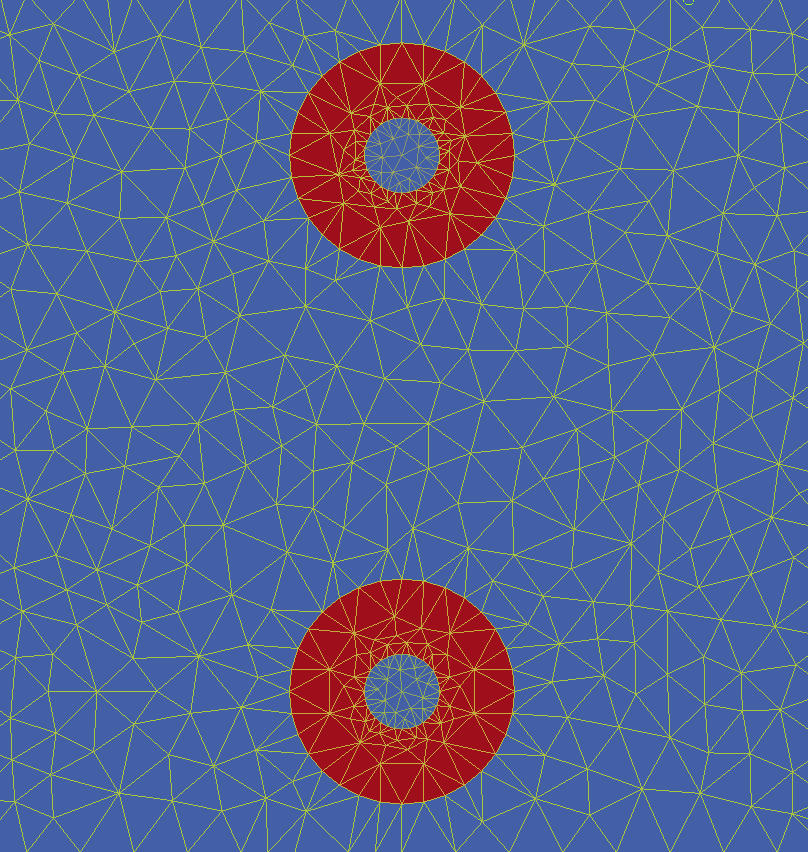
\includegraphics[width = .8\textwidth]{2filimax}
\end{figure}

In Tabella \ref{tab:fili2d2} sono mostrate le forze in direzione $x$ e $y$ per i due fili confrontando i metodi di Maxwell e del PLV con il valore teorico dato dalla formula di Lorentz. In tabella si fa riferimento al filo a nord con il pedice "N" e al filo a sud con il pedice "S".

\begin{table}[htb]
\caption{Confronto tra i valori di forza ottenuti tramite superficie di Maxwell e PLV}
\label{tab:fili2d2}
\centering
\begin{tabular}{lcccc}
\toprule
Metodo & $F_{xN}$ (N) & $F_{yN}$ (N) & $F_{xS}$  (N) & $F_{yS}$ (N)\\
\midrule
Lorentz & 0 & -5849.45 & 0 & 5849.45 \\
Maxwell & 2.43 & -5850.10 & 3.43 & 5850.40\\
PLV & 2.94& -5849.19 & 0.18 & 5850.57\\
\bottomrule
\end{tabular}
\end{table}

I risultati evidenziano che in due dimensioni e implementando una trasformazione al contorno i metodi sono estremamente precisi. In tre dimensioni e con l'aggiunta di magneti permanenti l'accuratezza del calcolo ottenuto peggiora notevolmente.

\subsection{Test-case: due magneti sferici in 3D}

Si illustra qui il risultato ottenuto confrontando tutti i metodi fin qui descritti per ottenere le forze scambiate tra due magneti di forma sferica con magnetizzazione costante, opposta e parallela alla retta che congiunge i centri delle due sfere. I dati geometrici utilizzati sono elencati in Tabella \ref{tab:2sfere} 

\begin{figure}[htb]
\centering
\caption{Porzioni della mesh racchiuse dalle superfici di Maxwell; la magnetizzazione  è costante (in direzione $x$), uguale ed opposta per le due sfere}
\label{fig:2sfere}
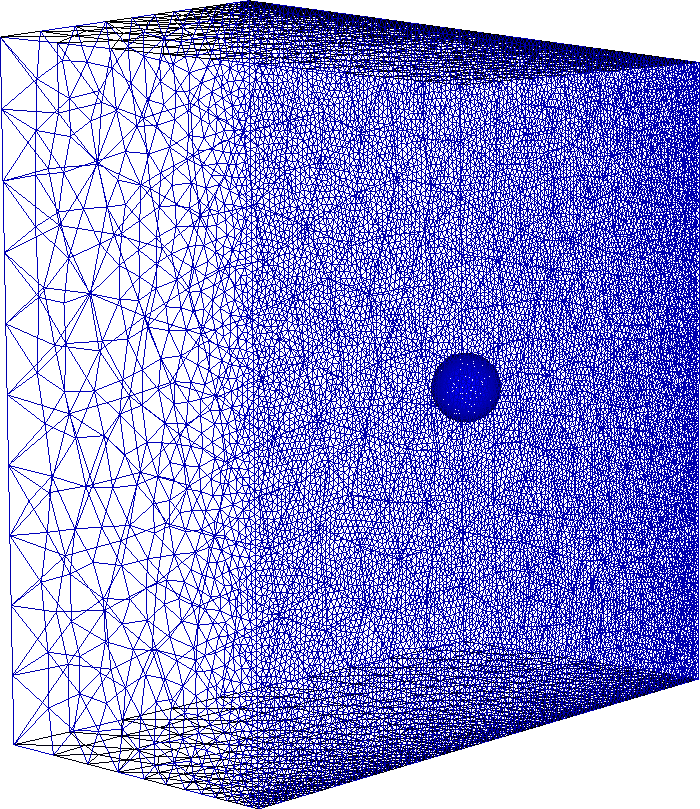
\includegraphics[width = .4\textwidth]{2sfere_a}
\quad 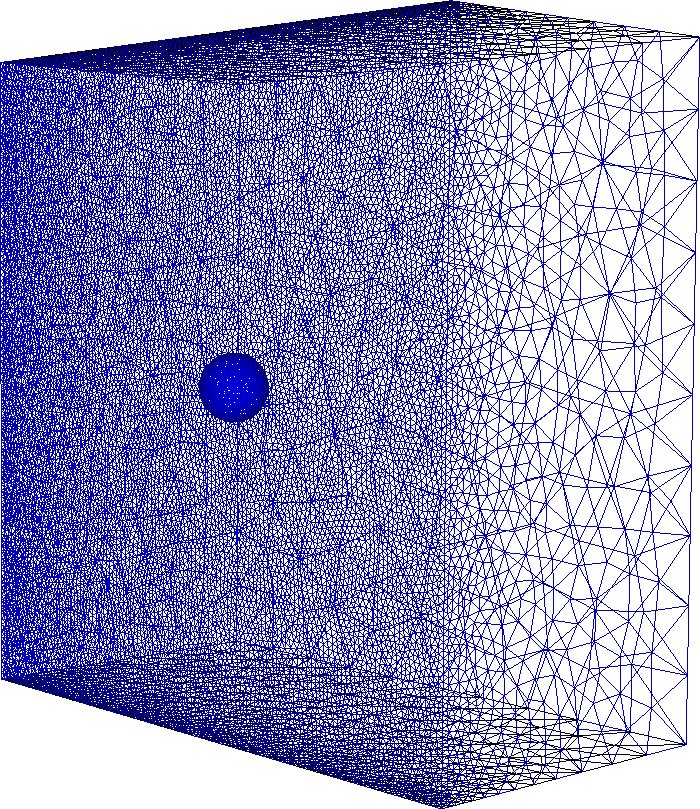
\includegraphics[width = .4\textwidth]{2sfere_b}
\end{figure}

\begin{table}[htb]
\caption{Dati geometrici utilizzati per il caso test}
\label{tab:2sfere}
\centering
\begin{tabular}{lc}
\toprule
Raggio sfere & \begin{tabular}{cc}$r$ & 0.25 m\end{tabular}\\
Distanza tra i centri delle sfere & \begin{tabular}{cc}$d$ & 1.5 m\end{tabular}\\
Campo magnetico residuo & \begin{tabular}{cc}$\T{b_r}$ & 1.36 T\end{tabular}\\
Superficie di Maxwell (Prisma) & $5m\times 10m\times 10m$\\
\bottomrule
\end{tabular}
\end{table}

In Tabella \ref{tab:2sfere2} sono mostrate le forze nelle tre direzioni. Si fa riferimento alla sfera sinistra con il pedice "S" e quella destra con il pedice "D".\\

\begin{table}[htb]
\caption{Confronto tra i valori di forza ottenuti tramite superficie di Maxwell e PLV}
\label{tab:2sfere2}
\centering
\footnotesize
\begin{tabular}{lcccccc}
\toprule
Metodo & $F_{xS}$ (N) & $F_{yS}$ (N) & $F_{zS}$  (N) & $F_{xD}$ (N) & $F_{yD}$ (N) & $F_{zD}$ (N)\\
\midrule
Cariche eq. & -38595.97 & 304.06 & -679.87 & 38993.11 & 994.46 & -383.75\\
Correnti eq. & -37636.58 & -235.01 & -526.97 & 38017.24 & 60.50 & -1075.37\\
Maxwell & -40686.41 & 1.91 & 13.63 & 40616.31 & -3.93 & -5.30\\
PLV  & -38925.57 & -64.81 & -187.87 & 38994.73 & -72.24 & -312.95\\
\bottomrule
\end{tabular}
\end{table}

Poiché in questo caso non sono disponibili risultati teorici o sperimentali, la qualità dei risultati è stata valutata in base ai seguenti parametri:
\begin{description}
\item[Simmetria] Per tutti i metodi utilizzati viene analizzata la differenza fra le forze $F_x$ agenti sulle due sfere. In tutti i casi l'errore percentuale $e = |F_{xS}-F_{xD}|/max(F_{xS},F_{xD})$ è accettabile:
\begin{center}\begin{tabular}{lc}
\toprule
Metodo & errore (\%)\\
\midrule
Cariche eq. & 1.02\\
Correnti eq. & 1.00\\
Maxwell & 0.17\\
PLV & 0.18\\
\bottomrule
\end{tabular}\end{center}
\item[Forze trasversali] La presenza di componenti non nulle in direzione $y$ e $z$ indica un errore, da attribuire in parte alle imperfezioni nella geometria della griglia di calcolo, in parte alla natura stessa dei metodi utilizzati. Di seguito è mostrato il rapporto fra le forze trasversali e quella longitudinale (il maggiore fra quelli ottenuti per le due sfere):
\begin{center}\begin{tabular}{lcc}
\toprule
Metodo & $\frac{F_y}{F_x}$ (\%) & $\frac{F_z}{F_x}$ (\%)\\
\midrule
Cariche eq. & 2.55 & 1.74\\
Correnti eq. & 0.62 & 12.82\\
Maxwell & 0.01 & 0.03\\
PLV & 0.16 & 0.8\\
\bottomrule
\end{tabular}\end{center}
\end{description}

\begin{figure}[htb]
\centering
\caption{Soluzione ottenuta: linee di flusso dell'induzione magnetica $\T{b}$}
\label{fig:2sfere2}
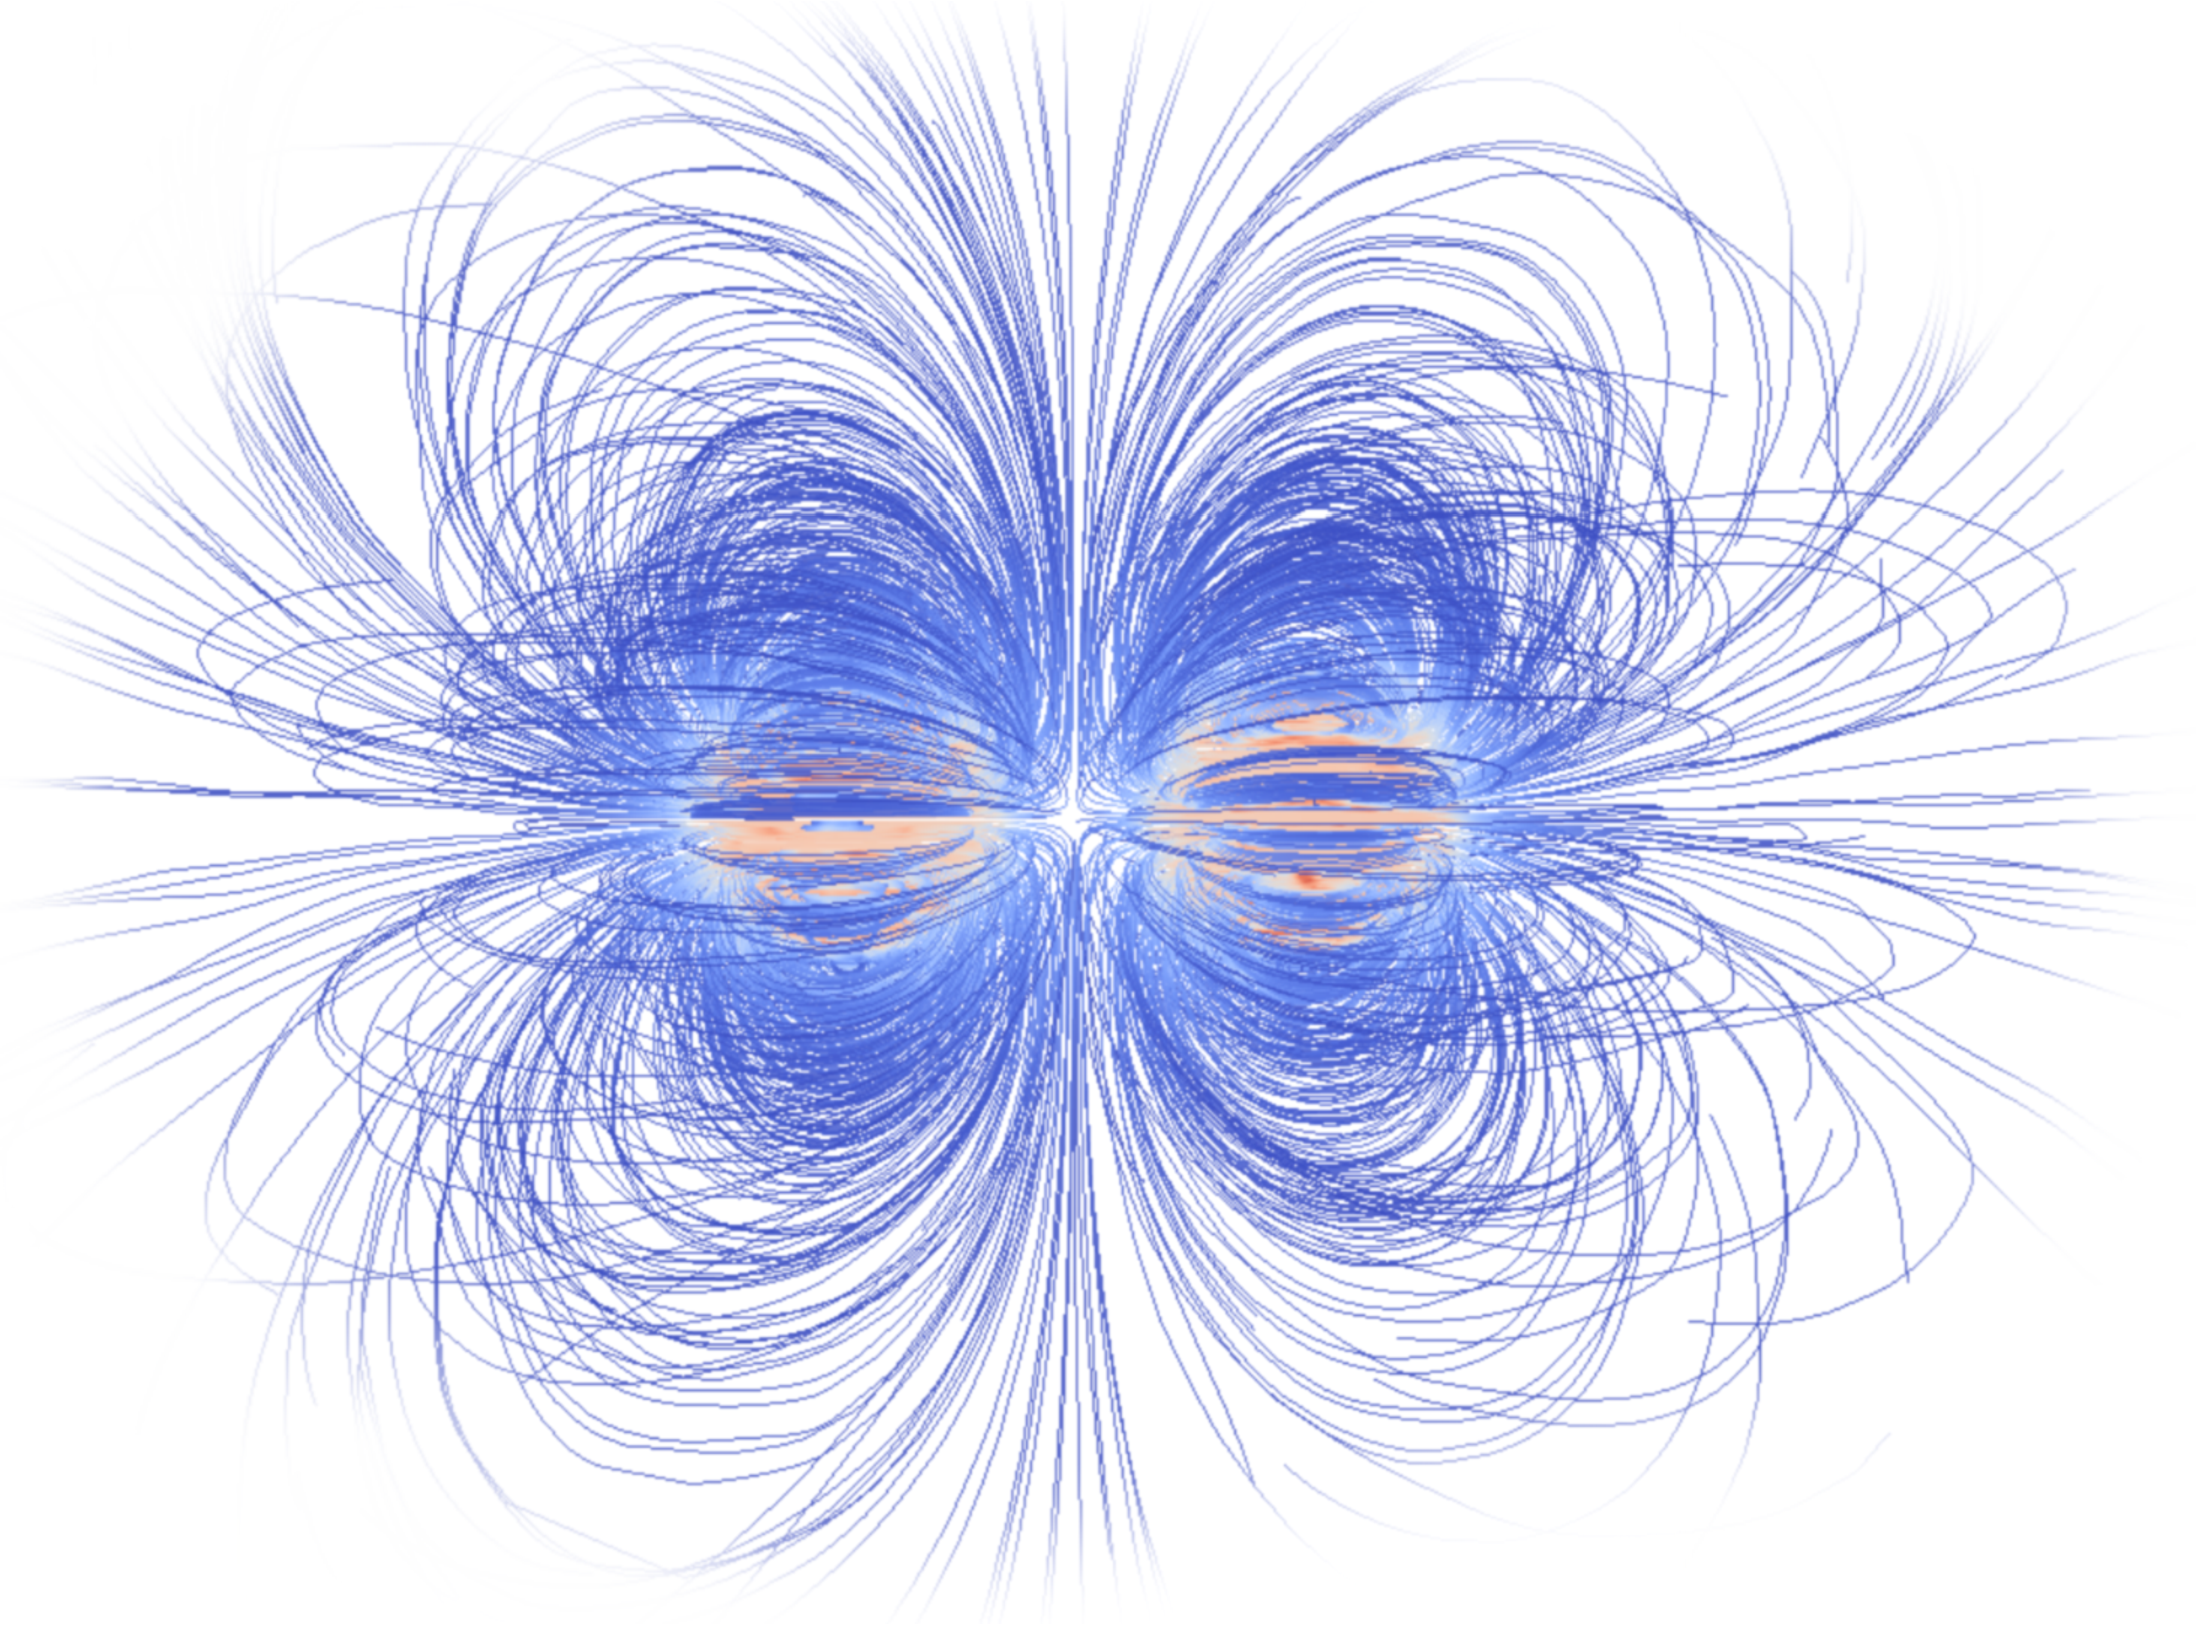
\includegraphics[width = \textwidth]{2sfere2}
\end{figure}

Come si può vedere, i metodi che mostrano gli errori minori sono il metodo del PLV e il metodo della superficie di Maxwell. Si noti infine un'anomalia: quest'ultimo metodo mostra un risultato maggiore del 2.5\% rispetto agli altri. 

Questo risultato mostra come, in base alla scelta della superficie il risultato possa variare sensibilmente.

Infatti la presenza di spigoli (in questo caso inserita di proposito) comporta  l'introduzione di un errore sistematico.\\

Lo stesso problema nasce se la superficie è troppo vicina ai corpi da analizzare. Una possibile soluzione per limitare questo effetto (oltre agli accorgimenti precedentemente elencati) è l'aumento dell'ordine degli elementi di Nèdèlec. Questa operazione  è estremamente costosa in termini computazionali e non è stata provata.


\subsection{Test-case: due magneti di un servomotore lineare}
Come ultimo caso, si valuta l'analisi delle forze scambiate fra due magneti permanenti che fanno parte di un servomotore lineare utilizzato per alcuni sistemi di ottica adattiva attualmente in uso. Per una descrizione dettagliata della forma dei magneti si rimanda alle sezioni \textit{shell magnet} e \textit{bias magnet} nel Capitolo \ref{chap:ActSens}. Le caratteristiche geometriche dei due magneti sono brevemente descritte in Tabella \ref{tab:2shellbiasdata}. 

\begin{SCtable}[1.][htb]
\centering
\caption{Dimensioni e caratteristiche dei magneti permanenti}
\label{tab:2shellbiasdata}
\begin{tabular}{lc}
\toprule
Magnete 1  &\\
\midrule
Raggio \textit{core} &  4 mm\\
Raggio esterno petali & 6.4 mm\\
Altezza & 4 mm\\
$B_r$ & 1.43 T\\
Direzione di $B_r$ \textit{core} & assiale\\
Direzione di $B_r$ petali & radiale (uscente)\\
\midrule
Magnete 2 &\\
Raggio interno & 0.75 mm\\
Raggio esterno & 1.5 mm\\
Altezza & 2 mm\\
$B_r$ & 1.17 T\\
Direzione di $B_r$ & assiale\\
\bottomrule
\end{tabular}
\end{SCtable}

In Figura \ref{fig:2shellbiasplots1} è mostrato l'andamento della forza scambiata tra i due magneti in direzione verticale (con riferimento alla Figura \ref{fig:2shellbiasmodel}) al variare della distanza \textit{face to face} tra i due magneti. Si può vedere dai dati sperimentali come l'andamento della forza sia corretto ma è necessario scalare i risultati di un fattore $f = 0.86$ per far coincidere le due curve. Questa differenza è attribuibile ad una induzione magnetica residua dei componenti diversa da quella nominale. Lo stesso comportamento è stato riscontrato per lo stesso caso anche con programmi commerciali.


\begin{figure}
\footnotesize
\centering
\caption{Elementi del modello in analisi}
\label{fig:2shellbiasmodel}
\begin{overpic}[width=0.6\textwidth,]{2magmodel}
\put(45,65){\textit{Core}}
\put(0,50){Petali}
\put(75,30){Magnete 1}
\put(30,10){Magnete 2}

\end{overpic}
\end{figure}


\begin{figure}
\footnotesize
\centering
 \begin{tikzpicture}
    \begin{axis}[axis y line = left,
                 grid = major,
                 axis x line = left,
    		     width = .8\textwidth,
                 ylabel = {Forze (N)}, 
                 xlabel = {Distanza verticale $z$ (mm)}]
    \addplot[samples = 200., smooth]
    file {./Immagini/Output/speforce.dat};
    \addplot[dashed, samples = 200, smooth]
    file {./Immagini/Output/comforce.dat};    
    \addplot[dashed, mark = *, samples = 200, smooth]
    file {./Immagini/Output/scaforce.dat};
    \legend{$sperimentale$\\$numerica$\\$numerica~scalata$\\}
    \end{axis}
    \end{tikzpicture}
\caption{Variazione della forza scambiata fra i magneti}
\label{fig:2shellbiasplots1}
\end{figure}

\section{Induttanza}
\label{sec:induttanza}
L'induttanza può essere calcolata in diversi modi a seconda della tipologia e della geometria degli elementi in gioco. In questo lavoro sono state implementate due differenti tecniche di calcolo:
\begin{itemize}
\item La prima tecnica, adatta a calcolare auto-induttanze e  mutue induttanze per geometrie relativamente semplici si basa sulla definizione stessa di flussi concatenati \citep{markus_zahn_electromagnetic_????}. Con riferimento alla Figura \ref{fig:5ind1} il flusso del campo magnetico $\T{b}$ attraverso la superficie $S$ racchiusa dalla linea $l$ è uguale alla circuitazione del potenziale vettoriale lungo $l$:

\begin{SCfigure}[2.4][htp]
\caption{Circuito lungo la linea $l$}
\label{fig:5ind1}
\tdplotsetmaincoords{55}{45}
\begin{tikzpicture}
	[scale=2,
		tdplot_main_coords,
		curve/.style={draw = black,fill = black!10!white, opacity = .7},
		curve2/.style={black,->}]
\def\R{.8} % sphere radius
\coordinate (O) at (0,0,0);
\coordinate (A) at (0,0,1);
\coordinate (B) at (\R,0,0);
\coordinate (C) at (\R,0.3*\R,0);
%draw the circle in the main frame
%\draw[->] {(B) -- (C)};
\draw {(0,0,-.25) -- (0,0,0)};
\draw {(.5*\R,0,-.25) -- (.5*\R,0,0)};
\draw {(-.5*\R,0,-.25) -- (-.5*\R,0,0)};
\draw {(0,.5*\R,-.25) -- (0,.5*\R,0)};
\draw {(0,-.5*\R,-.25) -- (0,-.5*\R,0)};
\draw {(0.5*\R,0.5*\R,-.25) -- (0.5*\R,0.5*\R,0)};
\draw {(-0.5*\R,-0.5*\R,-.25) -- (-0.5*\R,-0.5*\R,0)};
\tdplotdrawarc[curve]{(O)}{\R}{0}{360}{}{}
\tdplotdrawarc[curve2]{(O)}{\R*1.2}{360}{380}{}{}
\draw[->] {(0,0,0) -- (0,0,0.25)};
\draw[->] {(.5*\R,0,0) -- (.5*\R,0,0.25)};
\draw[->] {(-.5*\R,0,0) -- (-.5*\R,0,0.25)};
\draw[->] {(0,.5*\R,0) -- (0,.5*\R,0.25)};
\draw[->] {(0,-.5*\R,0) -- (0,-.5*\R,0.25)};
\draw[->] {(0.5*\R,0.5*\R,0) -- (0.5*\R,0.5*\R,0.25)};
\draw[->] {(-0.5*\R,-0.5*\R,0) -- (-0.5*\R,-0.5*\R,0.25)};

\draw (\R*1.3,0,0) node[right] {$d\T{l}$}; %label
\draw (0,\R*1.1,0) node[right] {$l$}; %label
\draw (-\R*0.2,-\R*0.7,0) node[right] {$S$}; %label
\draw (0,0,0.3) node[right] {$\T{b}$}; %label

\end{tikzpicture}
\end{SCfigure}

\begin{equation}
\label{eq:5ind1}
\Phi(\T{b}) = \int_l \T{a} \cdot d\T{l}.
\end{equation}

Nel caso in cui il circuito sia un solenoide rappresentabile come una superficie per cui passano N avvolgimenti, si può scrivere, con riferimento alla Figura \ref{fig:5ind2}:

\begin{SCfigure}[2.4][htb]
\caption{Circuito solenoidale rappresentato da una superficie continua}
\label{fig:5ind2}
\tdplotsetmaincoords{55}{45}
\begin{tikzpicture}
	[scale=2,
		tdplot_main_coords,
		curve/.style={draw = black,fill = black!10!white, opacity = .7},
		curve2/.style={black,->}]
\def\R{.8} % sphere radius
\coordinate (O) at (0,0,0);
\coordinate (A) at (0,0,1);
\coordinate (B) at (\R,0,0);
\coordinate (C) at (\R,0.3*\R,0);
%draw the circle in the main frame
%\draw[->] {(B) -- (C)};

\tdplotdrawarc[fill = white]{(0,0,-1)}{\R}{0}{360}{}{}
\tdplotdrawarc[fill = black!10!white, opacity = .7]{(0,0,-1)}{\R}{0}{360}{}{}
\fill[black!10!white, opacity = 0.7]{(-1.412/2*\R, -1.412/2*\R, 1) -- (-1.412/2*\R, -1.412/2*\R, -1) --(1.412/2*\R, 1.412/2*\R, -1) -- (1.412/2*\R, 1.412/2*\R, 1) -- (-1.412/2*\R, -1.412/2*\R, 1)};
\draw {(0,0,-1.25) -- (0,0,0)};
\draw {(.5*\R,0,-1.25) -- (.5*\R,0,0)};
\draw {(-.5*\R,0,-1.25) -- (-.5*\R,0,0)};
\draw {(0,.5*\R,-1.25) -- (0,.5*\R,0)};
\draw {(0,-.5*\R,-1.25) -- (0,-.5*\R,0)};
\draw {(0.5*\R,0.5*\R,-1.25) -- (0.5*\R,0.5*\R,0)};
\draw {(-0.5*\R,-0.5*\R,-1.25) -- (-0.5*\R,-0.5*\R,0)};
\tdplotdrawarc[curve2]{(A)}{\R*1.2}{90}{110}{}{}
\tdplotdrawarc[fill = white]{(0,0,1)}{\R}{0}{360}{}{}
\tdplotdrawarc[curve2]{(0,0,-.2)}{\R}{-125}{45}{}{}
\tdplotdrawarc[curve2]{(0,0,-.25)}{\R}{-125}{45}{}{}
\tdplotdrawarc[curve2]{(0,0,-.3)}{\R}{-125}{45}{}{}
\tdplotdrawarc[curve2]{(0,0,-.35)}{\R}{-125}{45}{}{}
\tdplotdrawarc[curve2]{(0,0,-.4)}{\R}{-125}{45}{}{}
\tdplotdrawarc[curve2]{(0,0,-.45)}{\R}{-125}{45}{}{}
\tdplotdrawarc[curve2]{(0,0,-.5)}{\R}{-125}{45}{}{}
\tdplotdrawarc[curve2]{(0,0,-.55)}{\R}{-125}{45}{}{}
\tdplotdrawarc[curve2]{(0,0,-.6)}{\R}{-125}{45}{}{}
\tdplotdrawarc[curve2]{(0,0,-.65)}{\R}{-125}{45}{}{}
\tdplotdrawarc[curve2]{(0,0,-.7)}{\R}{-125}{45}{}{}
\tdplotdrawarc[curve2]{(0,0,-.75)}{\R}{-125}{45}{}{}
\tdplotdrawarc[curve2]{(0,0,-.8)}{\R}{-125}{45}{}{}
\tdplotdrawarc[curve2]{(0,0,-.85)}{\R}{-125}{45}{}{}
\tdplotdrawarc[curve2]{(0,0,-.9)}{\R}{-125}{45}{}{}
\tdplotdrawarc[curve2]{(0,0,-.95)}{\R}{-125}{45}{}{}

\draw {(-1.412/2*\R, -1.412/2*\R, 1) -- (-1.412/2*\R, -1.412/2*\R, -1)};
\draw {(1.412/2*\R, 1.412/2*\R, 1) -- (1.412/2*\R, 1.412/2*\R, -1)};
\draw[->] {(0,0,0) -- (0,0,1.25)};
\draw[->] {(.5*\R,0,0) -- (.5*\R,0,1.25)};
\draw[->] {(-.5*\R,0,0) -- (-.5*\R,0,1.25)};
\draw[->] {(0,.5*\R,0) -- (0,.5*\R,1.25)};
\draw[->] {(0,-.5*\R,0) -- (0,-.5*\R,1.25)};
\draw[->] {(0.5*\R,0.5*\R,0) -- (0.5*\R,0.5*\R,1.25)};
\draw[->] {(-0.5*\R,-0.5*\R,0) -- (-0.5*\R,-0.5*\R,1.25)};

\draw[<->] {(-1.712/2*\R, -1.712/2*\R, 1) -- (-1.712/2*\R, -1.712/2*\R, -1)};
\draw (0,\R*1.3,1) node[right] {$d\T{l}$}; %label
\draw (0,\R*.6,-.7) node[right] {$l_k$}; %label
\draw (-\R*0.7,-\R*0.7,0) node[right] {$S$}; %label
\draw (-1.712/2*\R, -1.712/2*\R, 0) node[left] {$h$}; %label

\end{tikzpicture}
\end{SCfigure}

\begin{align}
\label{eq:5ind2}
\Phi(\T{b}) = \sum\limits_{k = 1}^{N} \int_{l_k} \T{a} \cdot d\T{l} &= N \frac{\int_h \int_l \T{a} \cdot d\T{l} dh}{\int_h dh}\nonumber\\
 &= \frac{N}{h} \int_S \T{a}\cdot \T{t} ds,
\end{align}
dove $S$ è la superficie del conduttore e $\T{t}$ è il versore tangente al filo in ciascun punto della superficie.

Infine, se il circuito è un solenoide con più strati di avvolgimenti, modellabile come volume continuo in cui scorrono N fili omogeneamente distribuiti, si può scrivere, con riferimento alla Figura \ref{fig:5ind3}:
\begin{align}
\label{eq:5ind3}
\Phi(\T{b}) = \sum\limits_{k = 1}^{N} \int_{l_k} \T{a} \cdot d\T{l} &= N \frac{\int_A \int_l \T{a} \cdot d\T{l} dA}{\int_A dA}\nonumber\\
&= \frac{N}{A} \int_V \T{a}\cdot \T{t} dV.
\end{align}


\begin{SCfigure}[2.4][htp]
\caption{Circuito solenoidale  multi-strato rappresentato da un volume continuo}
\label{fig:5ind3}
\tdplotsetmaincoords{55}{45}
\begin{tikzpicture}
	[scale=2,
		tdplot_main_coords,
		curve/.style={draw = black,fill = black!10!white, opacity = .7},
		curve2/.style={black,->}]
\def\R{.8} % sphere radius
\def\r{1.6}
\coordinate (O) at (0,0,0);
\coordinate (A) at (0,0,1);
\coordinate (B) at (\R,0,0);
\coordinate (C) at (\R,0.3*\R,0);
%draw the circle in the main frame
%\draw[->] {(B) -- (C)};
\tdplotdrawarc{(0,0,-1)}{\r}{45}{-135}{}{}
\tdplotdrawarc[draw = black, fill = black!10!white, opacity = .7]{(0,0,-1)}{\r}{-135}{45}{}{}
\draw [color = black!10!white, opacity = 0.3] {(-1.412/2*\R, -1.412/2*\R, -1) -- (0, 0, -1)};
\fill[black!10!white, opacity = 0.7]{(-1.412/2*\r, -1.412/2*\r, 1) -- (-1.412/2*\r, -1.412/2*\r, -1) --(1.412/2*\r, 1.412/2*\r, -1) -- (1.412/2*\r, 1.412/2*\r, 1) -- (-1.412/2*\r, -1.412/2*\r, 1)};
\tdplotdrawarc[fill = white]{(0,0,1)}{\r}{0}{360}{}{}
\tdplotdrawarc[ fill = black!10!white, opacity = .7]{(0,0,1)}{\r}{0}{360}{}{}
\tdplotdrawarc{(0,0,-1)}{\R}{0}{360}{}{}
\draw {(0,0,-1.25) -- (0,0,0)};
\draw {(.5*\R,0,-1.25) -- (.5*\R,0,0)};
\draw {(-.5*\R,0,-1.25) -- (-.5*\R,0,0)};
\draw {(0,.5*\R,-1.25) -- (0,.5*\R,0)};
\draw {(0,-.5*\R,-1.25) -- (0,-.5*\R,0)};
\draw {(0.5*\R,0.5*\R,-1.25) -- (0.5*\R,0.5*\R,0)};
\draw {(-0.5*\R,-0.5*\R,-1.25) -- (-0.5*\R,-0.5*\R,0)};
\tdplotdrawarc[curve2]{(A)}{\R*1.2}{90}{110}{}{}
\tdplotdrawarc[fill = white]{(0,0,1)}{\R}{0}{360}{}{}
\draw {(1.412/2*\R, 1.412/2*\R, 1) -- (1.412/2*\R, 1.412/2*\R, -1)};
\draw[dashed] {(-1.412/2*\R, -1.412/2*\R, 1) -- (-1.412/2*\R, -1.412/2*\R, -1)};
\draw {(-1.412/2*\r, -1.412/2*\r, 1) -- (-1.412/2*\r, -1.412/2*\r, -1)};
\draw {(1.412/2*\r, 1.412/2*\r, 1) -- (1.412/2*\r, 1.412/2*\r, -1)};
\draw[dashed] {(-1.412/2*\r, -1.412/2*\r, 1) -- (-1.412/2*\R, -1.412/2*\R, 1)};
\draw[dashed] {(-1.412/2*\r, -1.412/2*\r, -1) -- (-1.412/2*\R, -1.412/2*\R, -1)};
\draw[->] {(0,0,0) -- (0,0,1.25)};
\draw[->] {(.5*\R,0,0) -- (.5*\R,0,1.25)};
\draw[->] {(-.5*\R,0,0) -- (-.5*\R,0,1.25)};
\draw[->] {(0,.5*\R,0) -- (0,.5*\R,1.25)};
\draw[->] {(0,-.5*\R,0) -- (0,-.5*\R,1.25)};
\draw[->] {(0.5*\R,0.5*\R,0) -- (0.5*\R,0.5*\R,1.25)};
\draw[->] {(-0.5*\R,-0.5*\R,0) -- (-0.5*\R,-0.5*\R,1.25)};
\tdplotdrawarc[curve2]{(0,0,-.2)}{\R*1.5}{-40}{90}{}{}
\tdplotdrawarc[curve2]{(0,0,-.25)}{\R*1.3}{-40}{90}{}{}
\tdplotdrawarc[curve2]{(0,0,-.3)}{\R*1.5}{-40}{90}{}{}
\tdplotdrawarc[curve2]{(0,0,-.35)}{\R*1.3}{-40}{90}{}{}
\tdplotdrawarc[curve2]{(0,0,-.4)}{\R*1.5}{-40}{90}{}{}
\tdplotdrawarc[curve2]{(0,0,-.45)}{\R*1.3}{-40}{90}{}{}
\tdplotdrawarc[curve2]{(0,0,-.5)}{\R*1.5}{-40}{90}{}{}
\tdplotdrawarc[curve2]{(0,0,-.55)}{\R*1.3}{-40}{90}{}{}
\tdplotdrawarc[curve2]{(0,0,-.6)}{\R*1.5}{-40}{90}{}{}
\tdplotdrawarc[curve2]{(0,0,-.65)}{\R*1.3}{-40}{90}{}{}
\tdplotdrawarc[curve2]{(0,0,-.7)}{\R*1.5}{-40}{90}{}{}
\tdplotdrawarc[curve2]{(0,0,-.75)}{\R*1.3}{-40}{90}{}{}
\tdplotdrawarc[curve2]{(0,0,-.8)}{\R*1.5}{-40}{90}{}{}
\tdplotdrawarc[curve2]{(0,0,-.85)}{\R*1.3}{-40}{90}{}{}
\tdplotdrawarc[curve2]{(0,0,-.9)}{\R*1.5}{-40}{90}{}{}
\tdplotdrawarc[curve2]{(0,0,-.95)}{\R*1.3}{-40}{90}{}{}
\tdplotdrawarc[curve2]{(0,0,-.2)}{\R*1.7}{-40}{90}{}{}
\tdplotdrawarc[curve2]{(0,0,-.25)}{\R*1.9}{-40}{90}{}{}
\tdplotdrawarc[curve2]{(0,0,-.3)}{\R*1.7}{-40}{90}{}{}
\tdplotdrawarc[curve2]{(0,0,-.35)}{\R*1.9}{-40}{90}{}{}
\tdplotdrawarc[curve2]{(0,0,-.4)}{\R*1.7}{-40}{90}{}{}
\tdplotdrawarc[curve2]{(0,0,-.45)}{\R*1.9}{-40}{90}{}{}
\tdplotdrawarc[curve2]{(0,0,-.5)}{\R*1.7}{-40}{90}{}{}
\tdplotdrawarc[curve2]{(0,0,-.55)}{\R*1.9}{-40}{90}{}{}
\tdplotdrawarc[curve2]{(0,0,-.6)}{\R*1.7}{-40}{90}{}{}
\tdplotdrawarc[curve2]{(0,0,-.65)}{\R*1.9}{-40}{90}{}{}
\tdplotdrawarc[curve2]{(0,0,-.7)}{\R*1.7}{-40}{90}{}{}
\tdplotdrawarc[curve2]{(0,0,-.75)}{\R*1.9}{-40}{90}{}{}
\tdplotdrawarc[curve2]{(0,0,-.8)}{\R*1.7}{-40}{90}{}{}
\tdplotdrawarc[curve2]{(0,0,-.85)}{\R*1.9}{-40}{90}{}{}
\tdplotdrawarc[curve2]{(0,0,-.9)}{\R*1.7}{-40}{90}{}{}
\tdplotdrawarc[curve2]{(0,0,-.95)}{\R*1.9}{-40}{90}{}{}
\draw (0,\R*1.3,1) node[right] {$d\T{l}$}; %label
\draw (-\R,-\R*1.6,0) node[right] {$A$}; %label
\draw (-\R*0.7,-\R*0.7,1) node[right] {$V$}; %label
\end{tikzpicture}
\end{SCfigure}

In questo modo è possibile calcolare il flusso concatenato ad un circuito indipendentemente dalla sorgente del campo magnetico. Opportunamente utilizzata, questa tecnica permette quindi il calcolo, oltre che di auto-induttanze, anche di mutue induttanze e contro-tensioni originate da magneti in movimento (come attuatori lineari e motori).
\item La seconda tecnica si limita al calcolo di auto-induttanze ma è applicabile a qualunque circuito indipendentemente dalla complessità geometrica. Si basa sull'espressione dell'energia magnetica, che per un circuito induttivo può essere espressa  in dipendenza dai campi oppure in funzione dell'auto-induttanza $L$ \citep{furlani_permanent_2001}:
\begin{align}
\label{eq:5ind4a}
W &= \frac{1}{2}\int_V \mu^{-1} \T{b}\cdot\T{b} dv\\
\label{eq:5ind4b}
&= \frac{1}{2} L i^2
\end{align}
da cui:
\begin{equation}
\label{eq:5ind5}
L = \frac{1}{i^2} \int_V  \mu^{-1} \T{b}\cdot\T{b} dv.
\end{equation}
\end{itemize}

\subsection{Test-case: solenoidi coassiali a singolo avvolgimento}
Per validare le tecniche di calcolo dell'induttanza è stato progettato il seguente \textit{test-case}: due induttori cilindrici coassiali di uguale lunghezza $h$ appartenenti a due circuiti diversi accoppiano i diversi circuiti. La matrice delle induttanze che mostra l'accoppiamento è:
\begin{equation}
\label{eq:5ind6}
\TT{L} = \left[
\begin{array}{cc}
L_{11} & L_{12} \\L_{21} & L_{22}\end{array}\right].
\end{equation}

\begin{figure}[htb]
\centering
\caption{Sezione della mesh che mostra il campo magnetico costante all'interno dell'induttore (in rosso)}
\label{fig:2coil1}
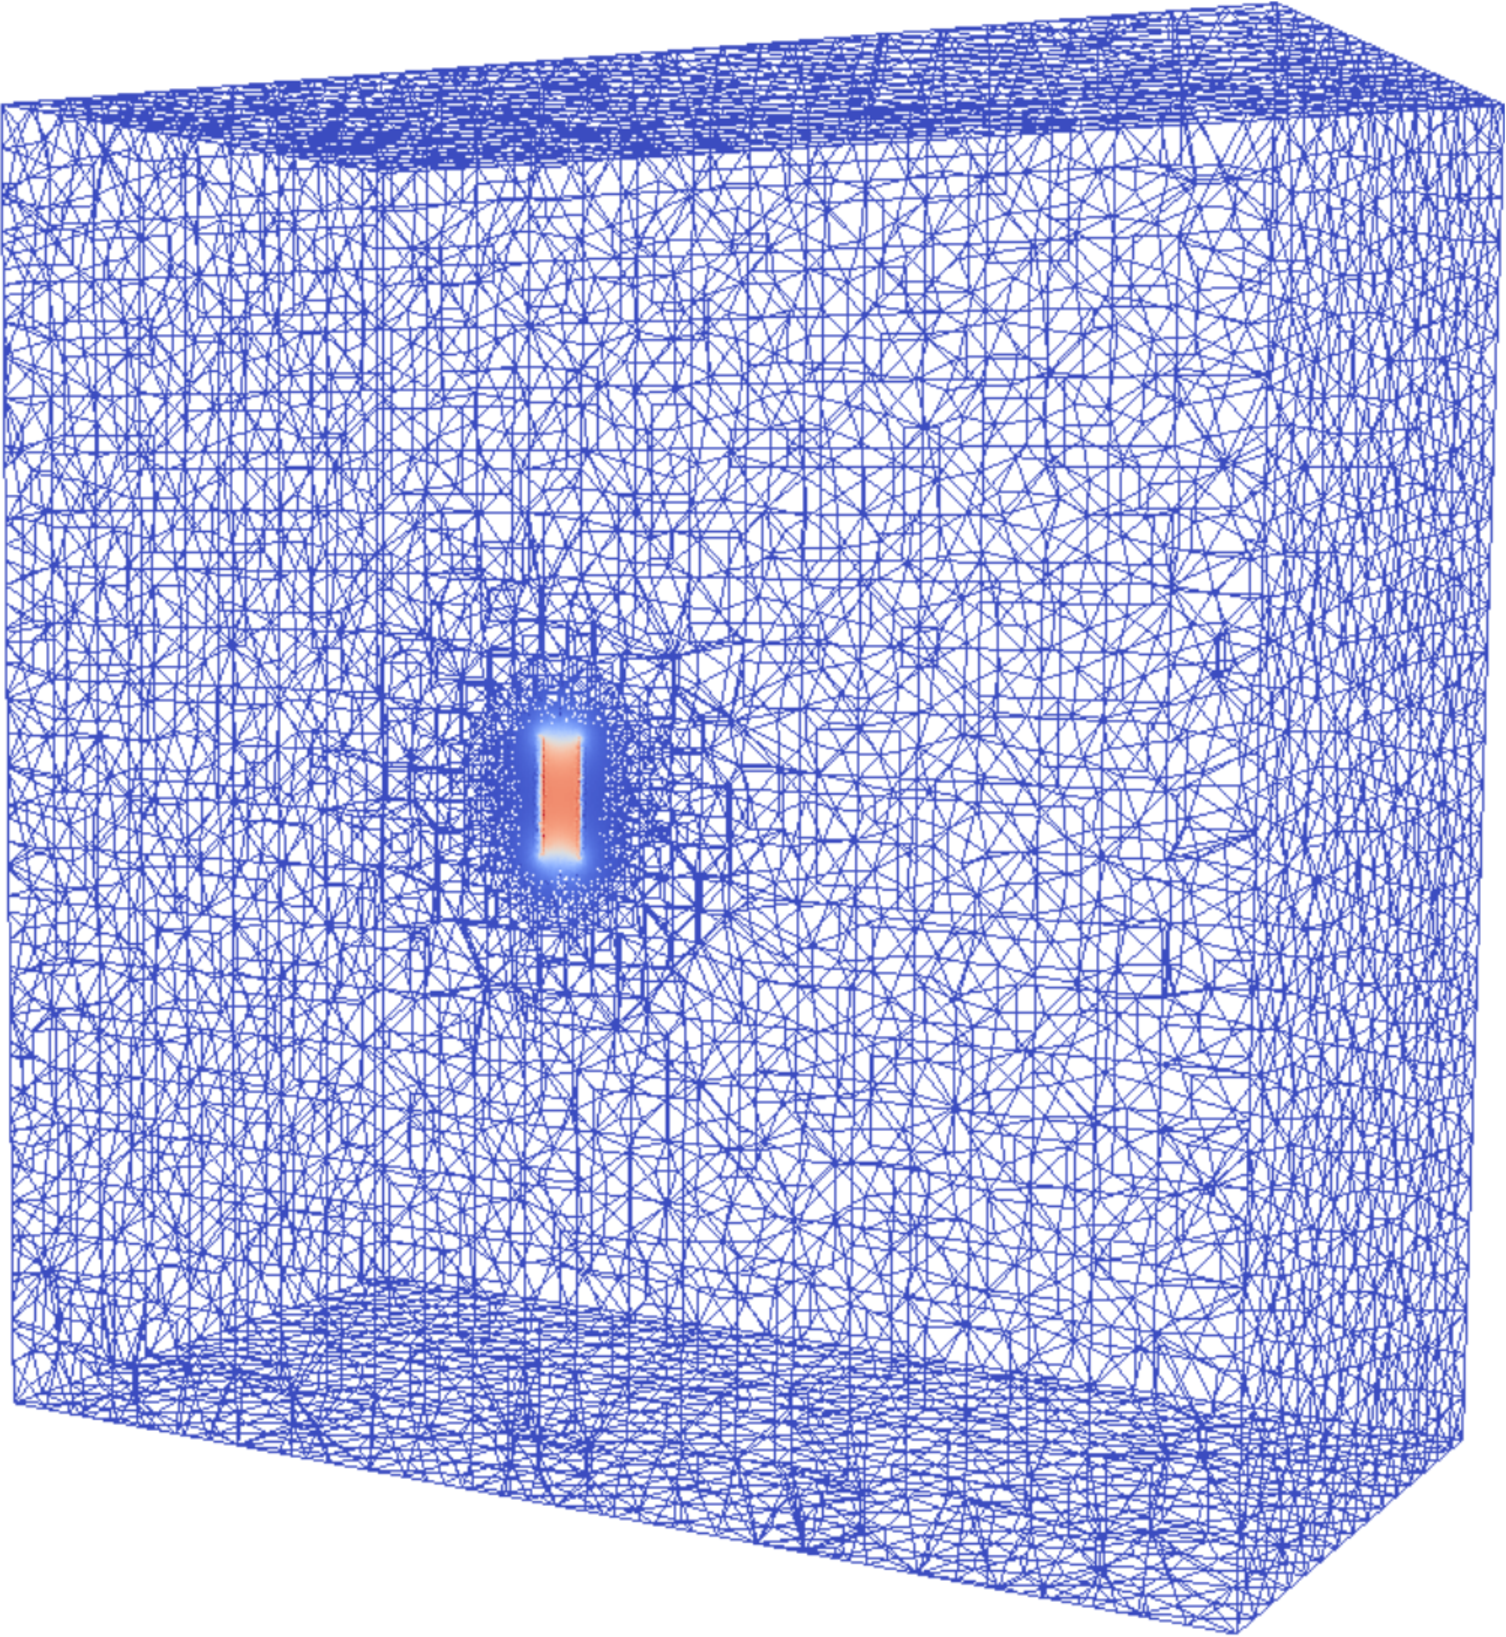
\includegraphics[width = .8\textwidth]{2coil2}
\end{figure}

\begin{table}[htb]
\caption{Dati geometrici utilizzati per i solenoidi}
\label{tab:2coil1}
\centering
\begin{tabular}{lccc}
\toprule
& Raggio $r$ & altezza $h$ & numero di spire $N$\\
\midrule
Avvolgimento 1 & .25 m& .05 m  & 1000\\
Avvolgimento 2 & .25 m& .07 m & 2000\\
\bottomrule
\end{tabular}
\end{table}

I dati del modello sono riportati in Tabella \ref{tab:2coil1}, mentre il confronto dei risultati ottenuti è mostrato in Tabella \ref{tab:2coil2}. Il valore teorico è stato ottenuto, soltanto per le auto-induttanze mediante la formula semi-empirica di Wheeler \citep{lee_integrated_2009}:
\begin{equation}
\label{eq:52coil1}
L_{ii} = 10 \mu_0 \frac{\pi~r_i^2 N_i^2}{9 r_i+10 h_i},
\end{equation}
dove l'induttanza è misurata in henry e le lunghezze in metri. Si riporta che la formula sopra citata è accompagnata da una tolleranza inferiore all'1\%.Come si può vedere, nel caso di auto-induttanze i risultati dei due metodi coincidono e mostrano uno scostamento inferiore allo 0.3 \%. 


\begin{figure}[htb]
\centering
\caption{Linee di flusso del campo magnetico attorno a uno dei due solenoidi}
\label{fig:2coil2}
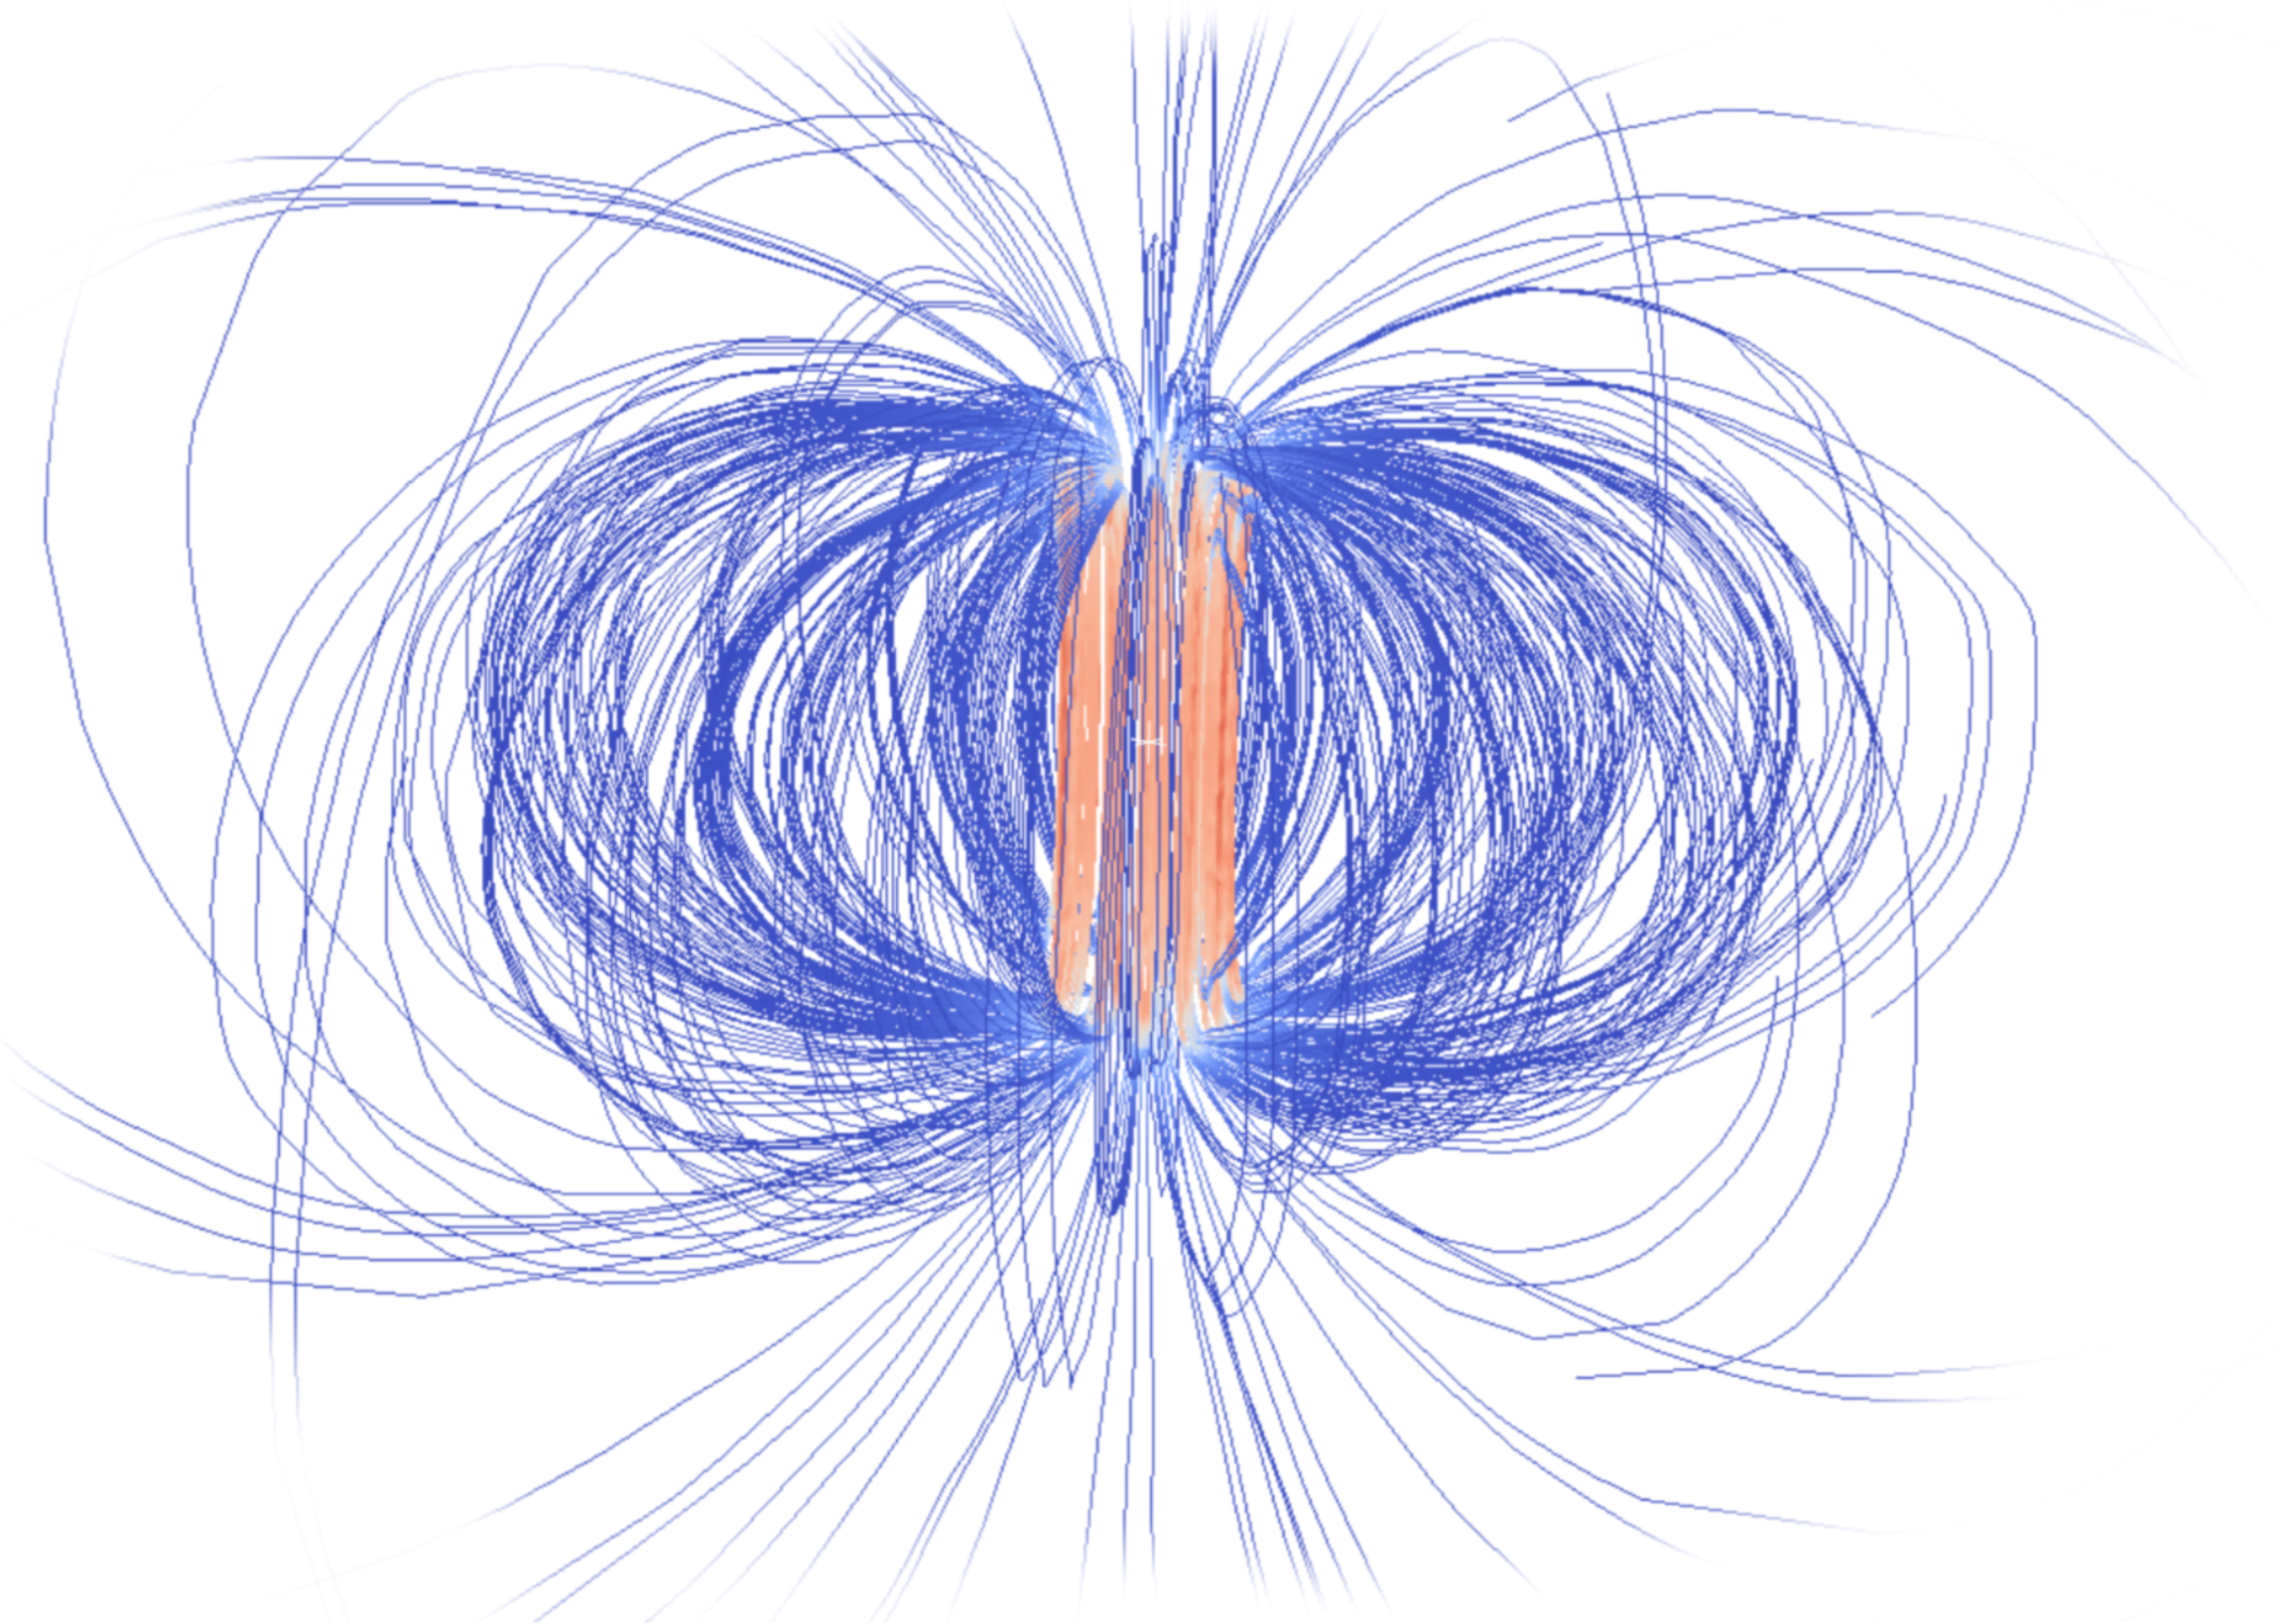
\includegraphics[width = \textwidth]{2coil1}
\end{figure}

\begin{table}[htb]
\caption{Confronto tra le induttanze}
\label{tab:2coil2}
\centering
\begin{tabular}{lcccc}
\toprule
 & Teorica & Primo metodo & Secondo metodo & errore\\
\midrule
$L_{11}$ (H)&  0.033456 & 0.033426& 0.033426& -0.09\%\\
$L_{12}$ (H)& -- & 0.061163 & -- & --\\
$L_{21}$ (H)&  --  & 0.061162& -- & --\\
$L_{22}$ (H)&  0.247213& 0.246676& 0.246676& -0.21\%\\
\bottomrule
\end{tabular}
\end{table}

\section{Capacità}
Il calcolo della capacità si è basato in questo lavoro sull'ipotesi di conduttori ideali. 

Infatti i sensori capacitivi utilizzati dai sistemi di controllo in esame in questo lavoro sono costituiti da rivestimenti aurei dello spessore dell'ordine del micrometro. Pertanto, vista l'alta conducibilità e il basso spessore, le armature sono state modellate come superfici conduttive ideali. \'E stato sufficiente in questo modo applicare come condizione al contorno due diversi potenziali sulle superfici. 

\'E in questo modo sufficiente applicare la definizione generale di capacità \citep{markus_zahn_electromagnetic_????}:
\begin{align}
\label{eq:5cap1}
C &= \frac{q_{1_{tot}}}{\Delta\phi} = \frac{\int_{S_1} -\T{d}\cdot{n} ds}{\int_l \T{e} \cdot d\T{l}}\nonumber\\
 &=\frac{q_{2_{tot}}}{\Delta\phi} = \frac{\int_{S_2} -\T{d}\cdot{n} ds}{\int_l \T{e} \cdot d\T{l}},
\end{align}
dove $S_1$ e $S_2$ sono le superfici conduttive delle armature dei condensatori e si è fatto utilizzo della condizione al contorno \eqref{eq:4pec_d}, utilizzando le normali mostrate in Figura \ref{fig:5cap1}.

\begin{SCfigure}[2.4][htp]
\caption{Riferimento per il calcolo della capacità utilizzando il potenziale elettrico}
\label{fig:5cap1}
\tdplotsetmaincoords{75}{45}
\begin{tikzpicture}
	[scale=2.5,
		tdplot_main_coords,
		curve/.style={draw = black,fill = black!10!white, opacity = .8}]
\def\R{.8} % sphere radius
\coordinate (O) at (0,0,0);
\coordinate (C) at (0,0,-.5);
\coordinate (P) at (0,0,.25);
\coordinate (Q) at (0,0,.75);
%draw the circle in the main frame
\draw[->] {(O) -- (C)};
\tdplotdrawarc[curve]{(O)}{\R}{0}{360}{}{}
\draw (C) node[right] {$\T{n}$}; %label

\tdplotdrawarc[curve]{(P)}{\R}{0}{360}{}{}
\draw[->] {(P) -- (Q)};
\draw (Q) node[right] {$\T{n}$}; %label
\draw (\R*.4,0,0) node[right] {$S_1$}; %label
\draw (\R*.4,0,.25) node[right] {$S_2$}; %label
\end{tikzpicture}
\end{SCfigure}

Ricordando ora l'equazione \eqref{eq:2max12s} si può scrivere:

\begin{equation}
\label{eq:5cap2}
C = \frac{\int_{S} \varepsilon\grad\left(\phi\right)\cdot\T{n}ds}{\Delta\phi} = \frac{\int_{S} \varepsilon\de_{\T{n}}\phi ~ ds}{\Delta\phi}.
\end{equation}

\subsection{Test-case: condensatore piano}
\begin{figure}[htb]
\centering
\caption{Parte della mesh e dettaglio della soluzione del potenziale elettrico}
\label{fig:cond1}
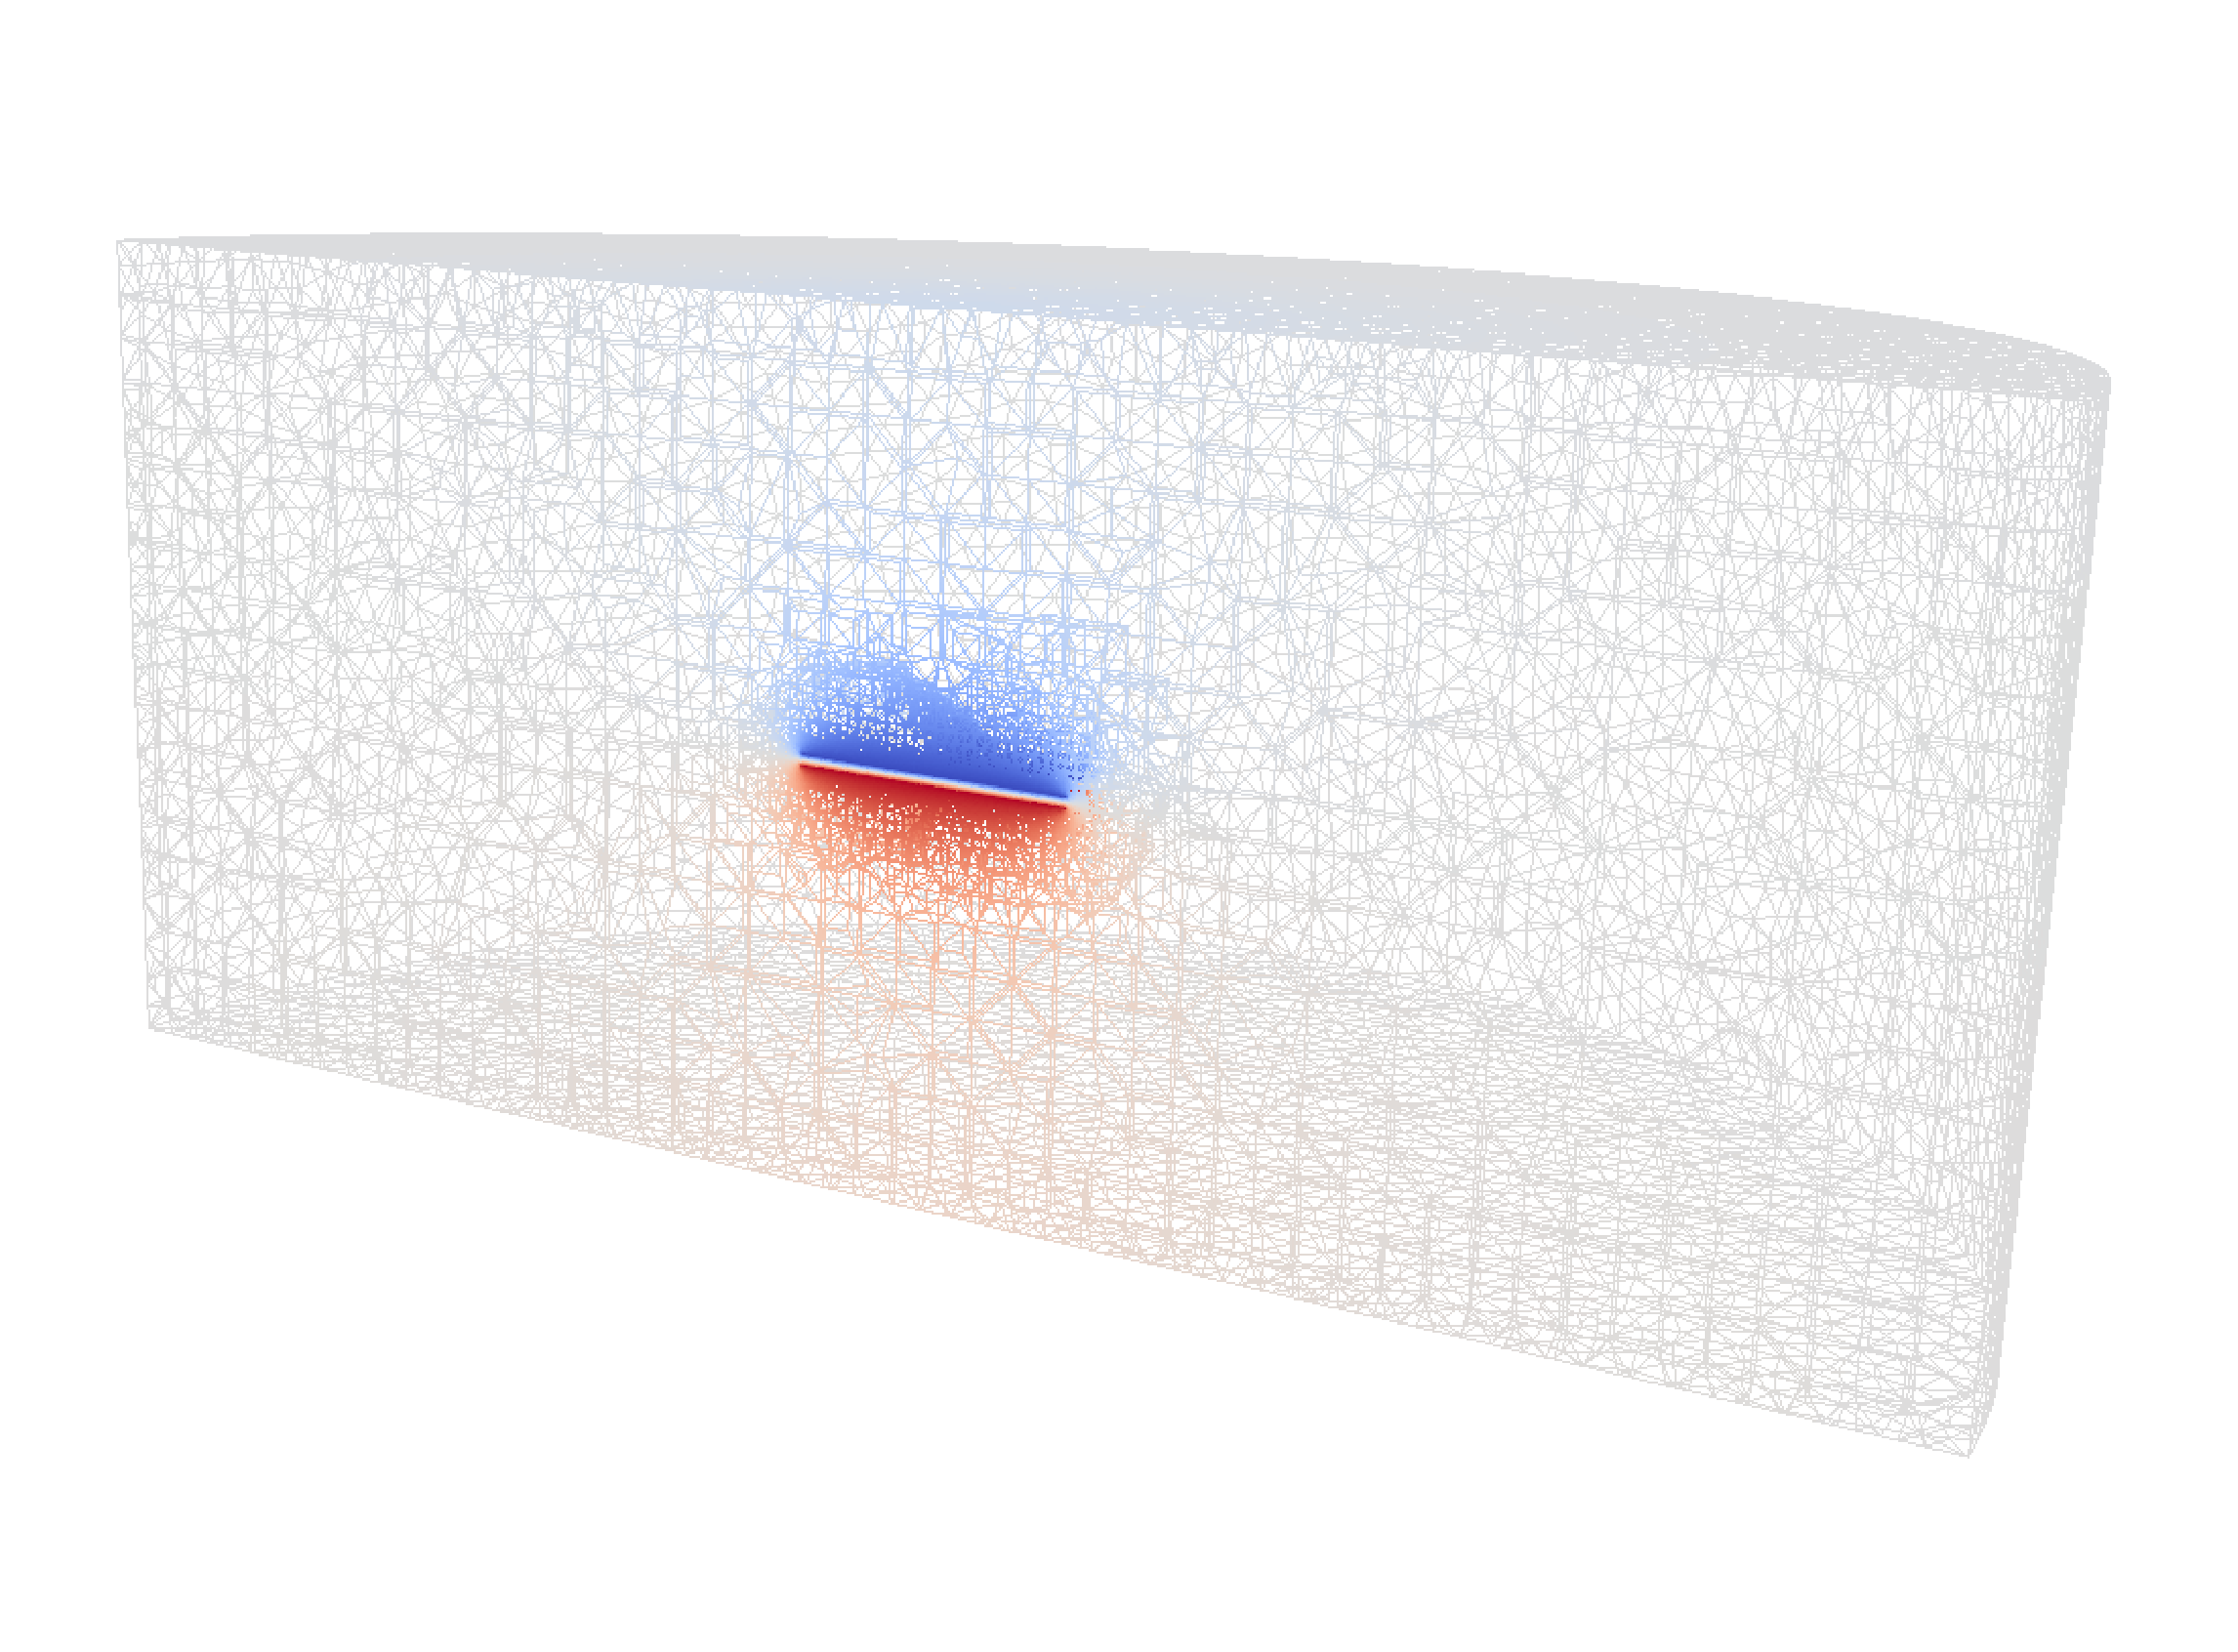
\includegraphics[width = .6\textwidth]{cond1}
\end{figure}

Si riporta come esempio il calcolo della capacità per un condensatore piano: due superfici circolari parallele sono poste ad una distanza $d$. Il volume racchiuso dalle due armature è occupato da aria. Se la distanza è piccola rispetto all'area delle armature, la capacità è data con ottima approssimazione da:
\begin{equation}
\label{eq:5cond1}
C = \varepsilon \frac{S}{d}.
\end{equation}

\begin{table}[htb]
\caption{Dati geometrici utilizzati per il condensatore}
\label{tab:5cond1}
\centering
\begin{tabular}{lcc}
\toprule
Raggio armature & $r$ & 20 mm\\
Area armature & $S$ & 1256.6 $\text{mm}^2$\\
Distanza armature & $d$ & 1.5 mm \\
\bottomrule
\end{tabular}
\end{table}

\begin{figure}[htb]
\centering
\caption{Dettaglio della soluzione: linee di flusso del campo elettrico $\T{e}$}
\label{fig:cond3}
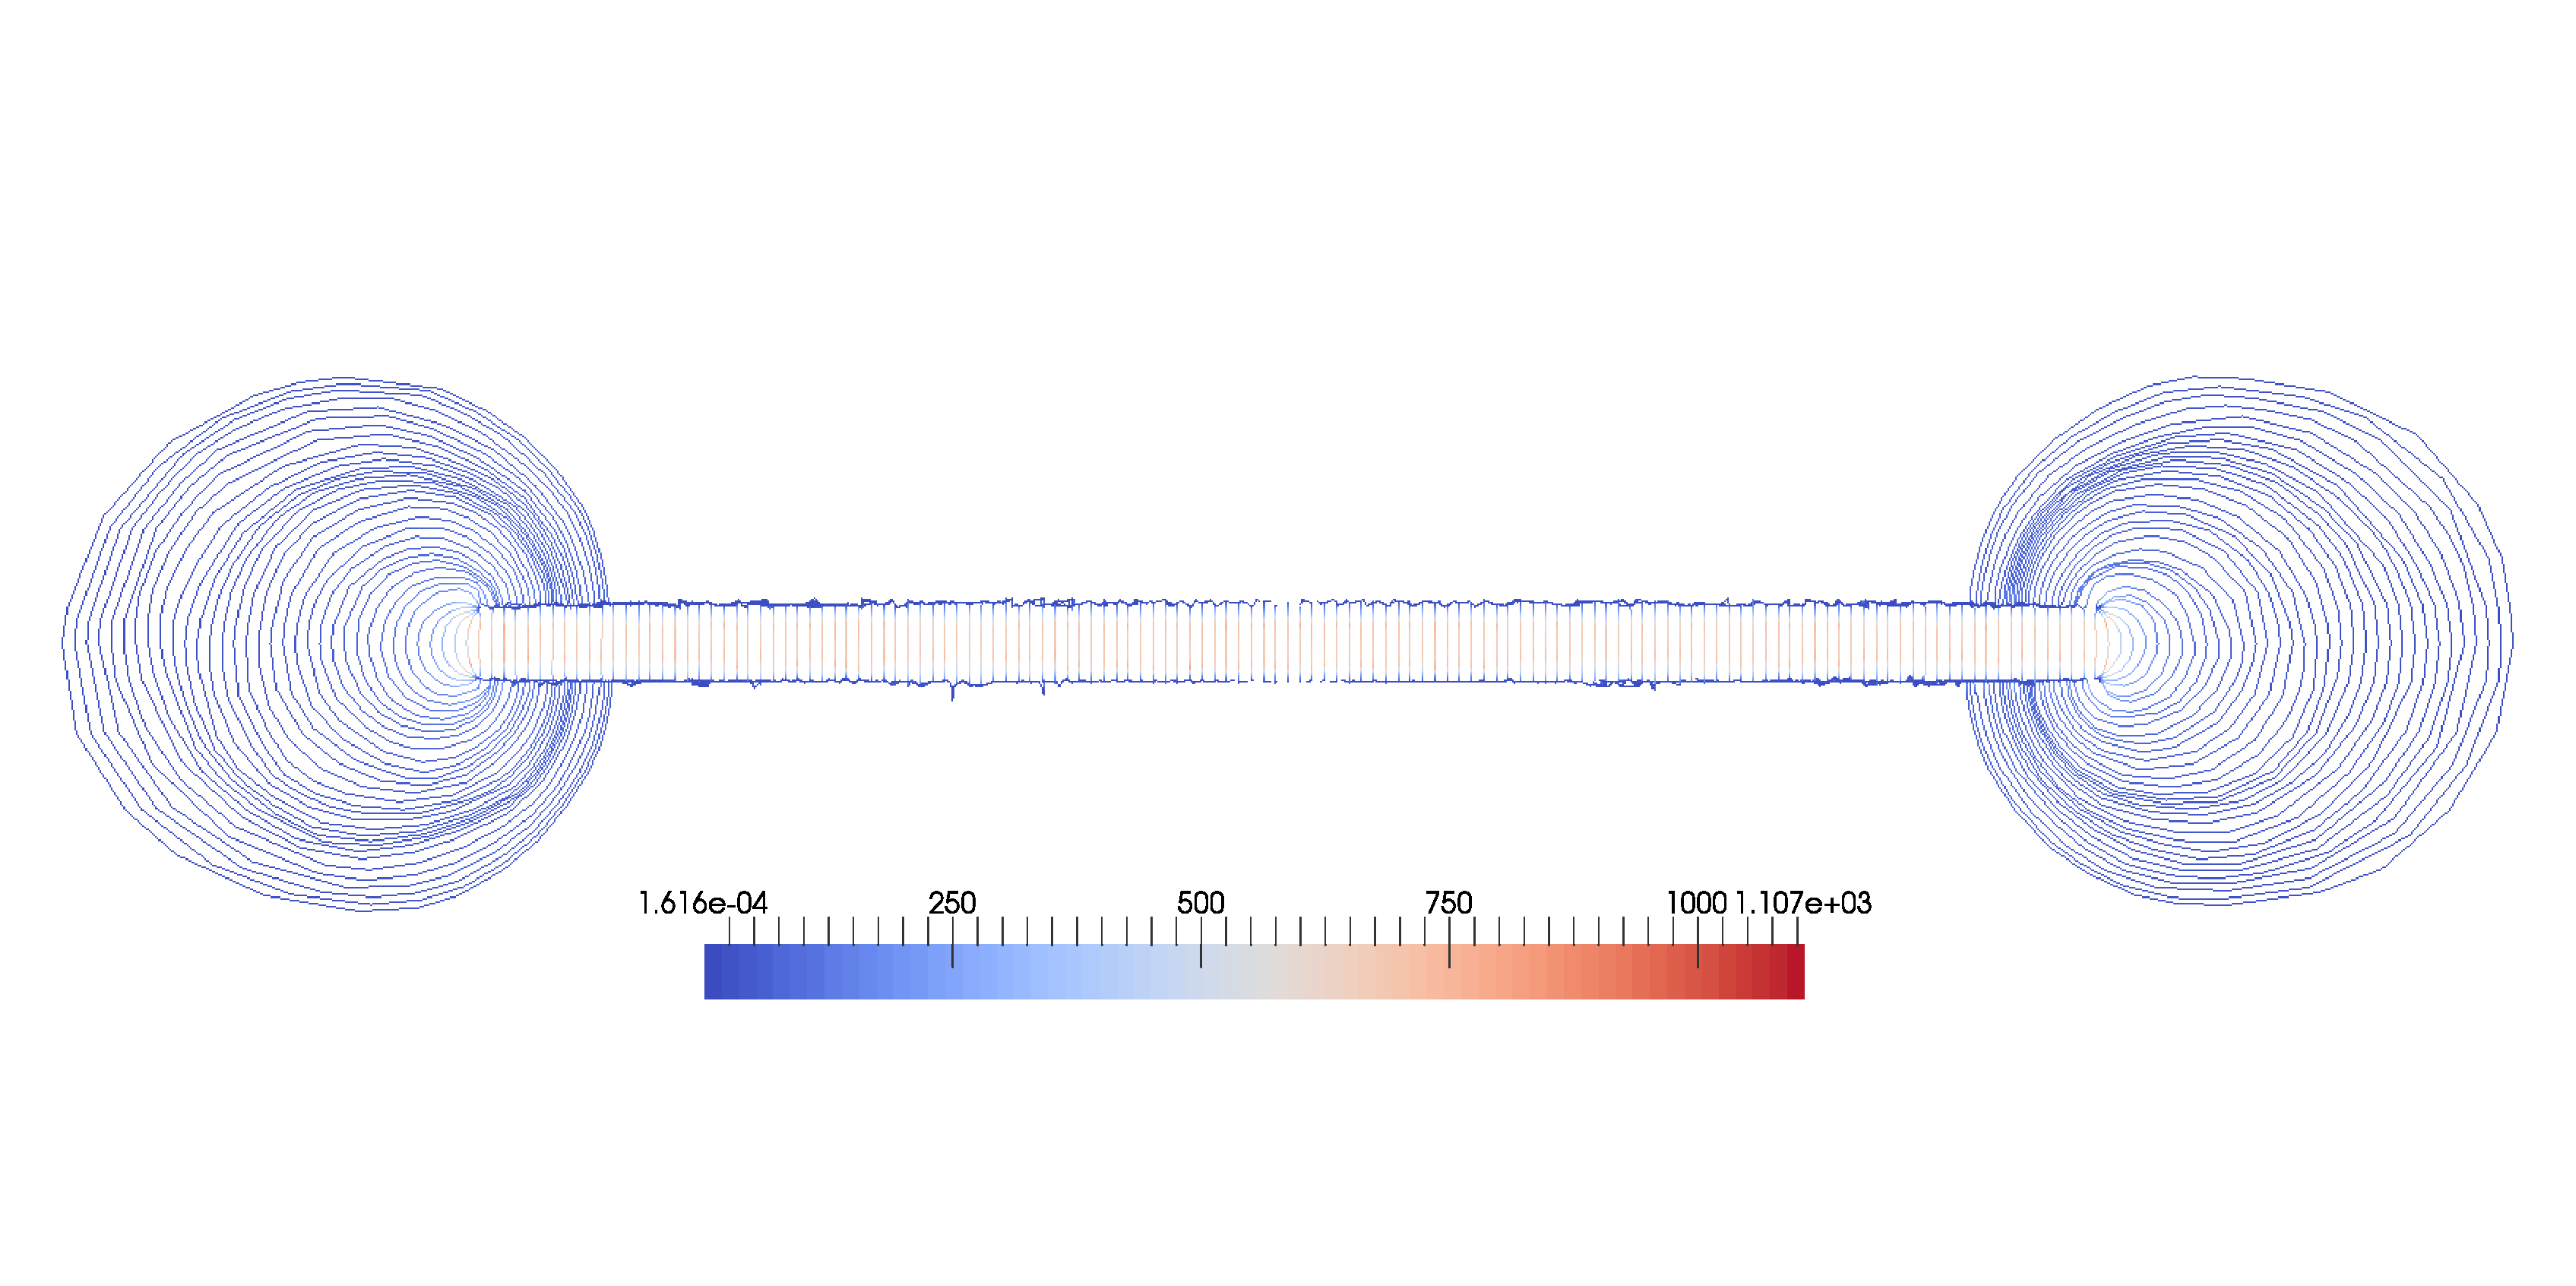
\includegraphics[width = \textwidth]{cond3}
\end{figure}

In Tabella \ref{tab:5cond1} sono mostrati i dati geometrici del modello.
Il confronto dei risultati è mostrato in tabella \ref{tab:5cond2}.
Come si può osservare, l'errore resta al di sotto del percentile; inoltre la differenza fra le integrazioni effettuate sulle due superfici è minima; il calcolo può pertanto essere effettuato soltanto su una delle due, scelta in base a regolarità e semplicità nell'integrazione.

\begin{table}[htb]
\caption{Confronto fra capacità teorica e calcolata}
\label{tab:5cond2}
\centering
\begin{tabular}{lcc}
\toprule
& Capacità (nF) & errore\\
\midrule
Teorica & 7.418 & --\\
Superficie 1 & 7.461 & 0.58 \%\\
Superficie 2 & 7.458 & 0.54 \%\\
\bottomrule
\end{tabular}
\end{table}
\cleardoublepage\part{Analisi degli elementi del sistema di controllo}
% !TEX encoding = UTF-8 Unicode
% !TEX TS-program = pdflatex
% !TEX root = ../Tesi.tex



%************************************************
\myChapter{Attuatori e sensori}
%************************************************
\label{chap:ActSens}
Una grande svolta nell'utilizzo di specchi attivi nell'osservazione astronomica è stata la realizzazione di sistemi di controllo basati su attuatori e sensori \textit{contactless} applicati ad uno specchio sospeso, tenuto in equilibrio unicamente dall'azione attiva del sistema di controllo e dalla rigidezza del sostegno centrale.

La configurazione ideale del sistema prevede la co-locazione di controlli e misure. La scelta del "dove e come acquisire e attuare" ha quindi come obiettivo l'avvicinamento dei due strumenti. Per questo ogni servomotore lineare è circondato da una corona circolare metallica che costituisce una delle due armature di un sensore capacitivo, mentre l'altra armatura è costituita da un rivestimento sullo specchio stesso. L'insieme di attuatore e sensore costituisce un'unità di controllo. Il numero di unità differisce da specchio a specchio; per gli specchi della generazione corrente si arriva anche ad alcune migliaia.

In questo capitolo viene analizzata la configurazione del sistema di attuazione e lettura M4 in fase di sviluppo per i telescopi GMT e E-ELT. Il progetto e i dati utilizzati in questo lavoro sono stati concessi da \textit{Microgate} (\textcopyright\url{www.microgate.it}).

\begin{figure}[htb]
\centering
\caption{Complessivo dell'unità di controllo M4}
\label{fig:M4assembly}
\begin{overpic}[width=\textwidth,]{M4_assembly}
\put(7,33){Superficie}
\put(9,31){specchio}
\put(16,26){Pot}
\put(9,13){Solenoide}
\put(66,8){Bias-magnet}
\put(75,22){Shell-magnet}
\put(84,33){Condensatore}
\put(75,31){Puk}
\end{overpic}
\end{figure}

Il servomotore del sistema è costituito da tre elementi principali: 

\begin{description}

\item[Shell-Magnet] Si tratta del componente solidale allo specchio deformabile ed è l'elemento più complesso del servomotore. \'E composto da diversi magneti in lega di neodimio-ferro-boro (materiale non conduttore con permeabilità magnetica $\mu = 1.05 \mu_0$) a magnetizzazione residua nominale $\T{b_r} = 1.43$ T. La struttura è così composta:
\begin{itemize}
\item Un magnete centrale cilindrico con magnetizzazione assiale;
\item Uno strato di colla dello spessore di 0.05 mm che riveste la superficie laterale del cilindro;
\item Otto magneti a settore di corona circolare di 44° con magnetizzazione radiale secondo la bisettrice del settore, incollati alla superficie laterale del cilindro e separati fra loro da uno strato di colla di 1°;
\item Un contenitore di alluminio (\textit{pot}) in cui è installato il complesso dei magneti.
\item Un elemento di separazione tra il \textit{pot} e la superficie inferiore dello specchio (\textit{puk}).
\end{itemize}

\begin{figure}[htb]
\centering
\caption{Geometria dei componenti dello shell-magnet: \textit{core} (a), \textit{sectors} (b), \textit{pot} (c) (\textcopyright Microgate)}
\label{fig:M4shellmagnet}
\subfloat[][]{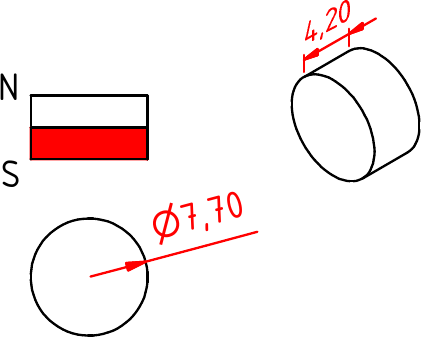
\includegraphics[width = .3\textwidth]{core}}\quad
\subfloat[][]{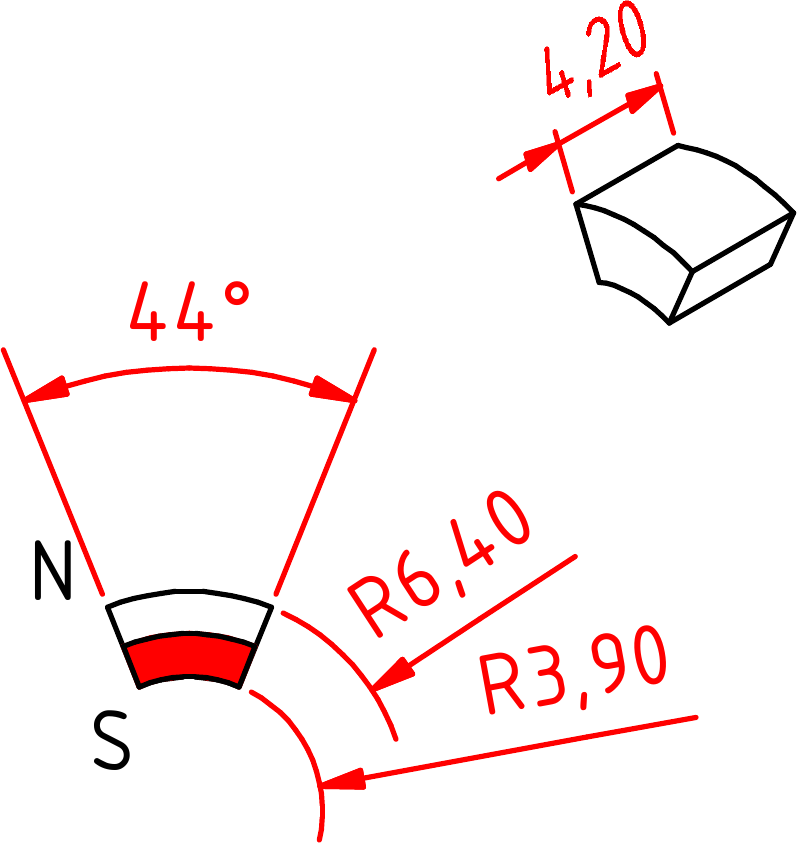
\includegraphics[width = .3\textwidth]{petals}}\quad
\subfloat[][]{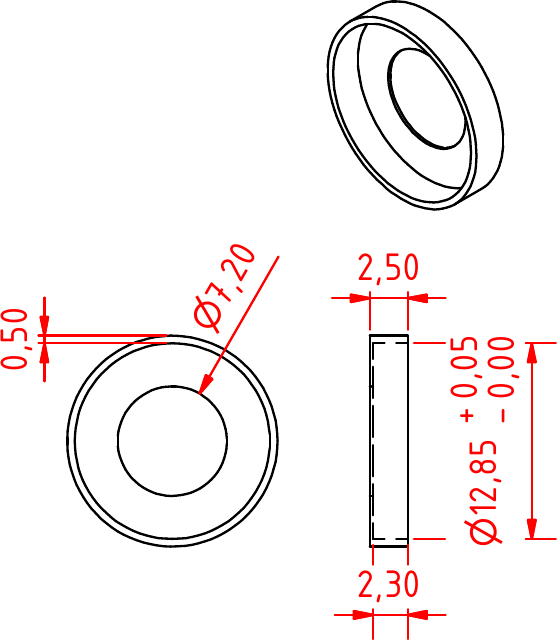
\includegraphics[width = .3\textwidth]{pot}}
\end{figure}

\begin{SCtable}[1.][htb]
\centering
\footnotesize
\caption{Dati geometrici del magnete solidale alla piastra}
\label{tab:M4shellmagnetdata}
\begin{tabular}{l}
\toprule
\textit{Core}\\
\midrule
\begin{tabular}{lc}
Raggio &  3.85 mm\\
Altezza &  4.2 mm\\
Materiale & NdFeB N52\\
\end{tabular}\\

\toprule
\textit{Settori}\\
\midrule
\begin{tabular}{lc}
Raggio interno  & 3.9 mm\\
Raggio esterno & 6.4 mm\\
Altezza & 4.2 mm\\
Materiale & NdFeB N52\\
\end{tabular}\\
\toprule
\textit{Pot}\\
\midrule
\begin{tabular}{lcc}
Raggio foro & 6.6 mm\\
Raggio esterno & 12.9 mm\\
Altezza & 2.5 mm\\
Spessore & 0.2 mm\\
Materiale & Al \\
\end{tabular}\\
\bottomrule
\end{tabular}
\end{SCtable}

I dati geometrici delle varie parti sono elencati in Tabella \ref{tab:M4shellmagnetdata}, mentre il campo magnetico generato dal magnete permanente è mostrato in Figura \ref{fig:M4shellmagnet1}.

\begin{figure}[htb]
\centering
\caption{Induzione magnetica dallo shell-magnet}
\label{fig:M4shellmagnet1}
\subfloat[][Sezione rispetto ad un diametro del magnete]{
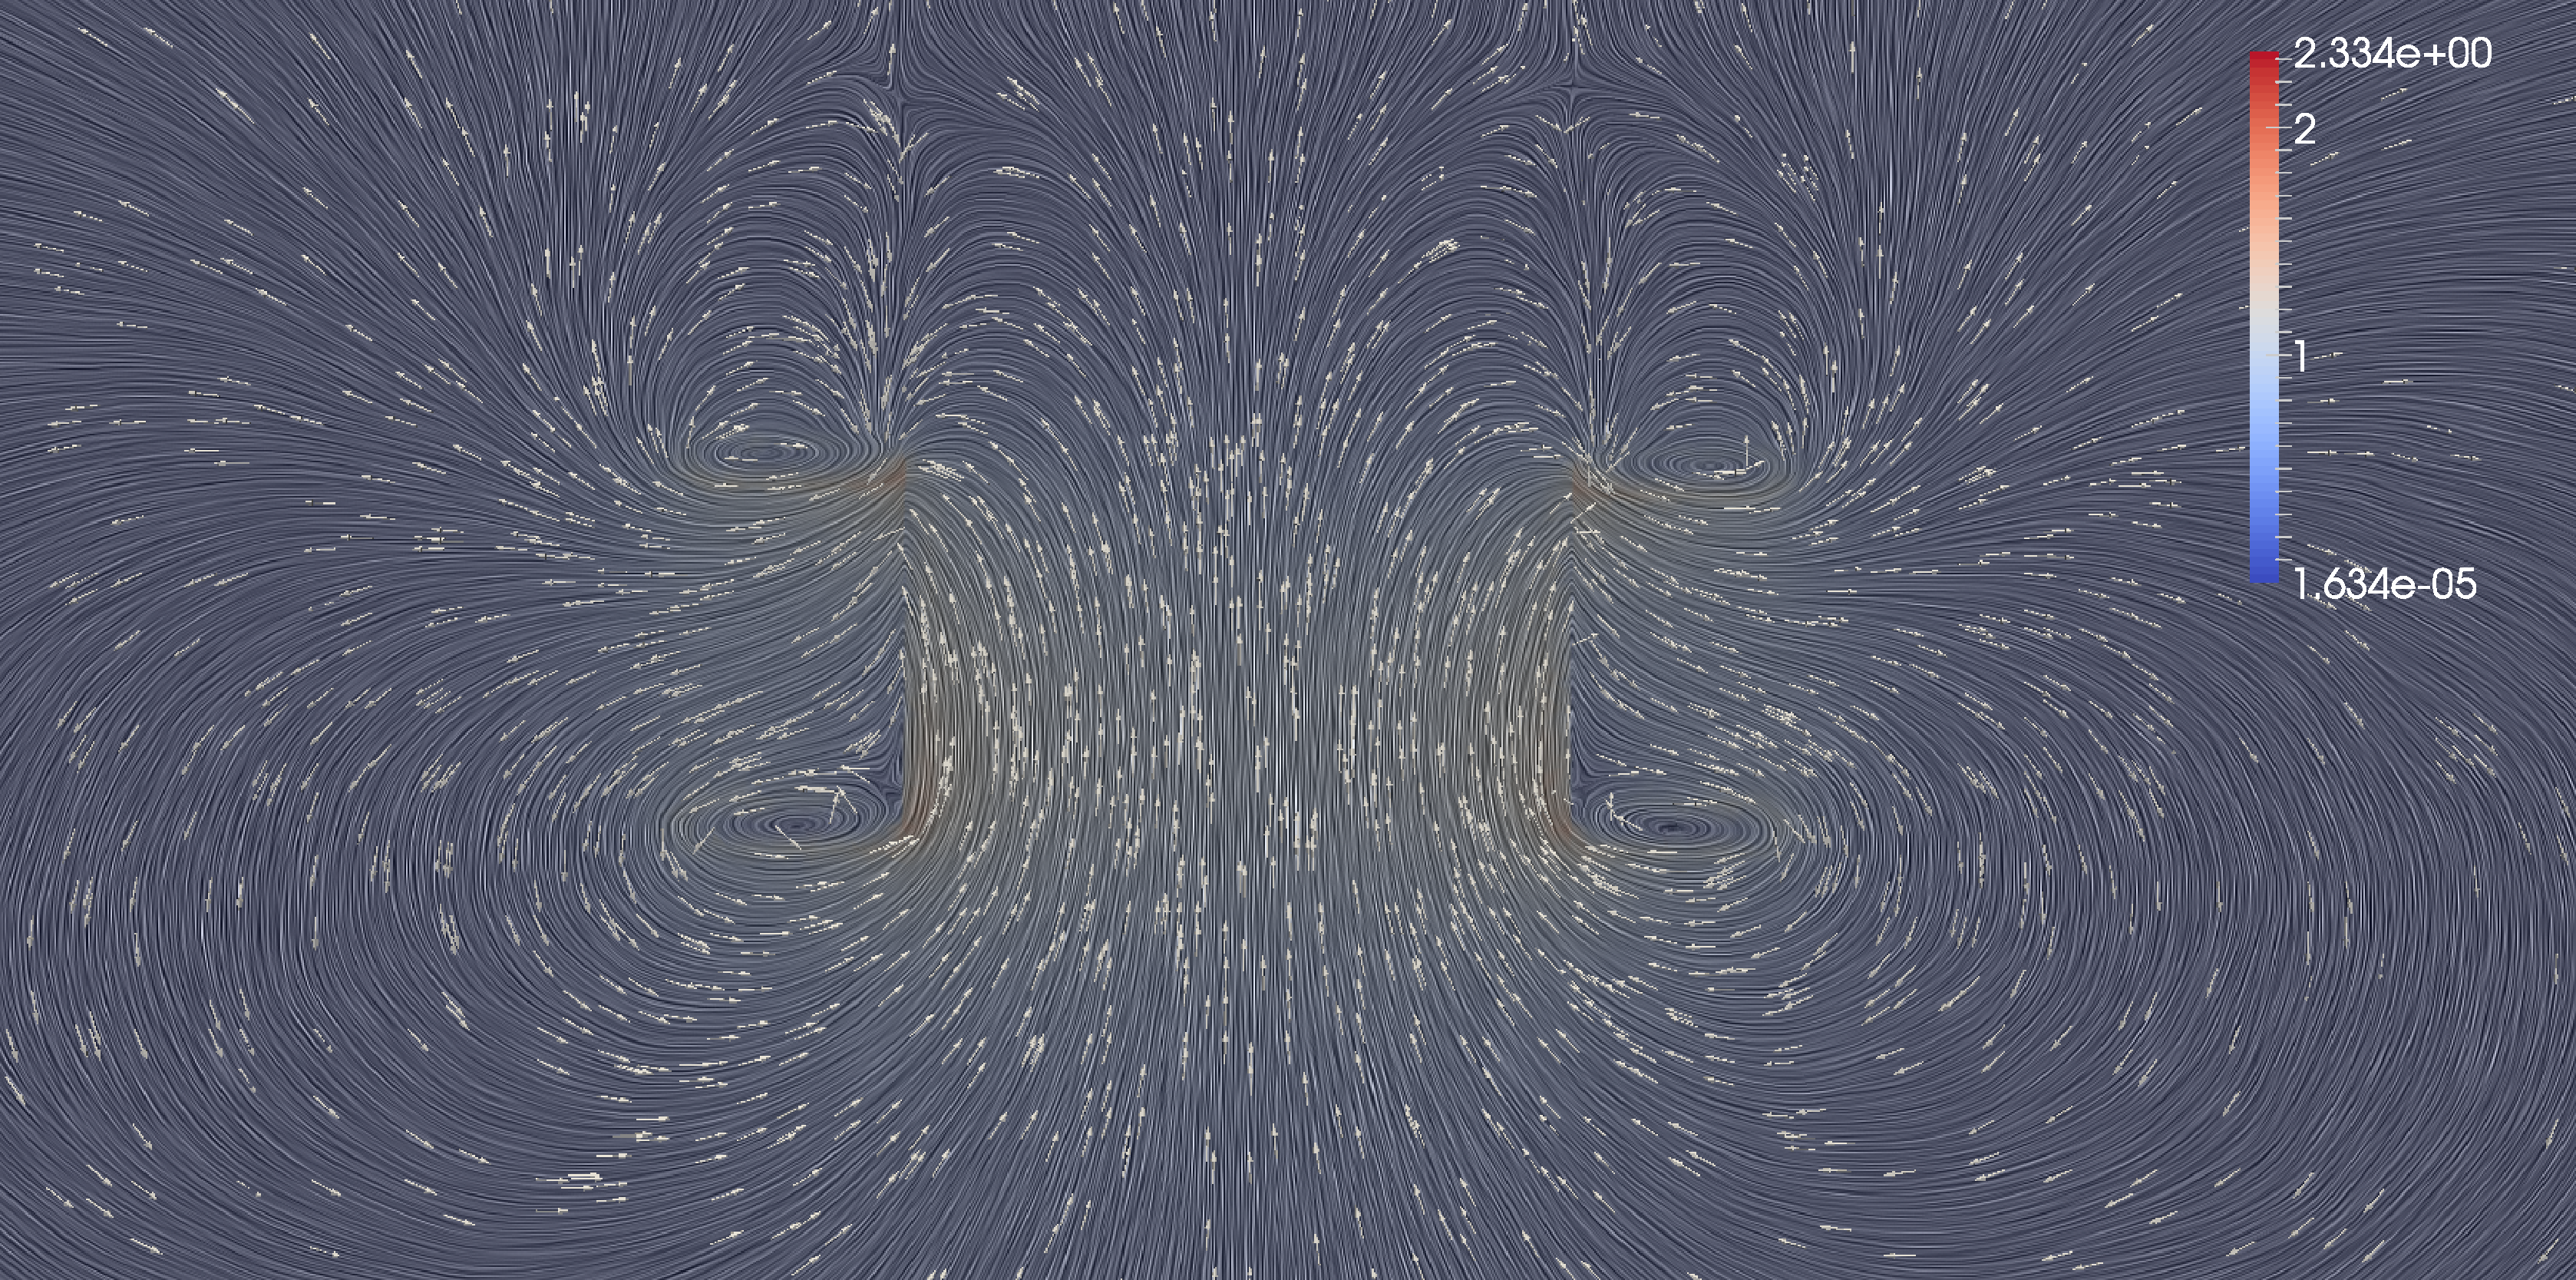
\includegraphics[width = .8\textwidth]{M4shellmagnet1}}
\\
\subfloat[][Dettaglio delle linee di flusso e della mesh]{
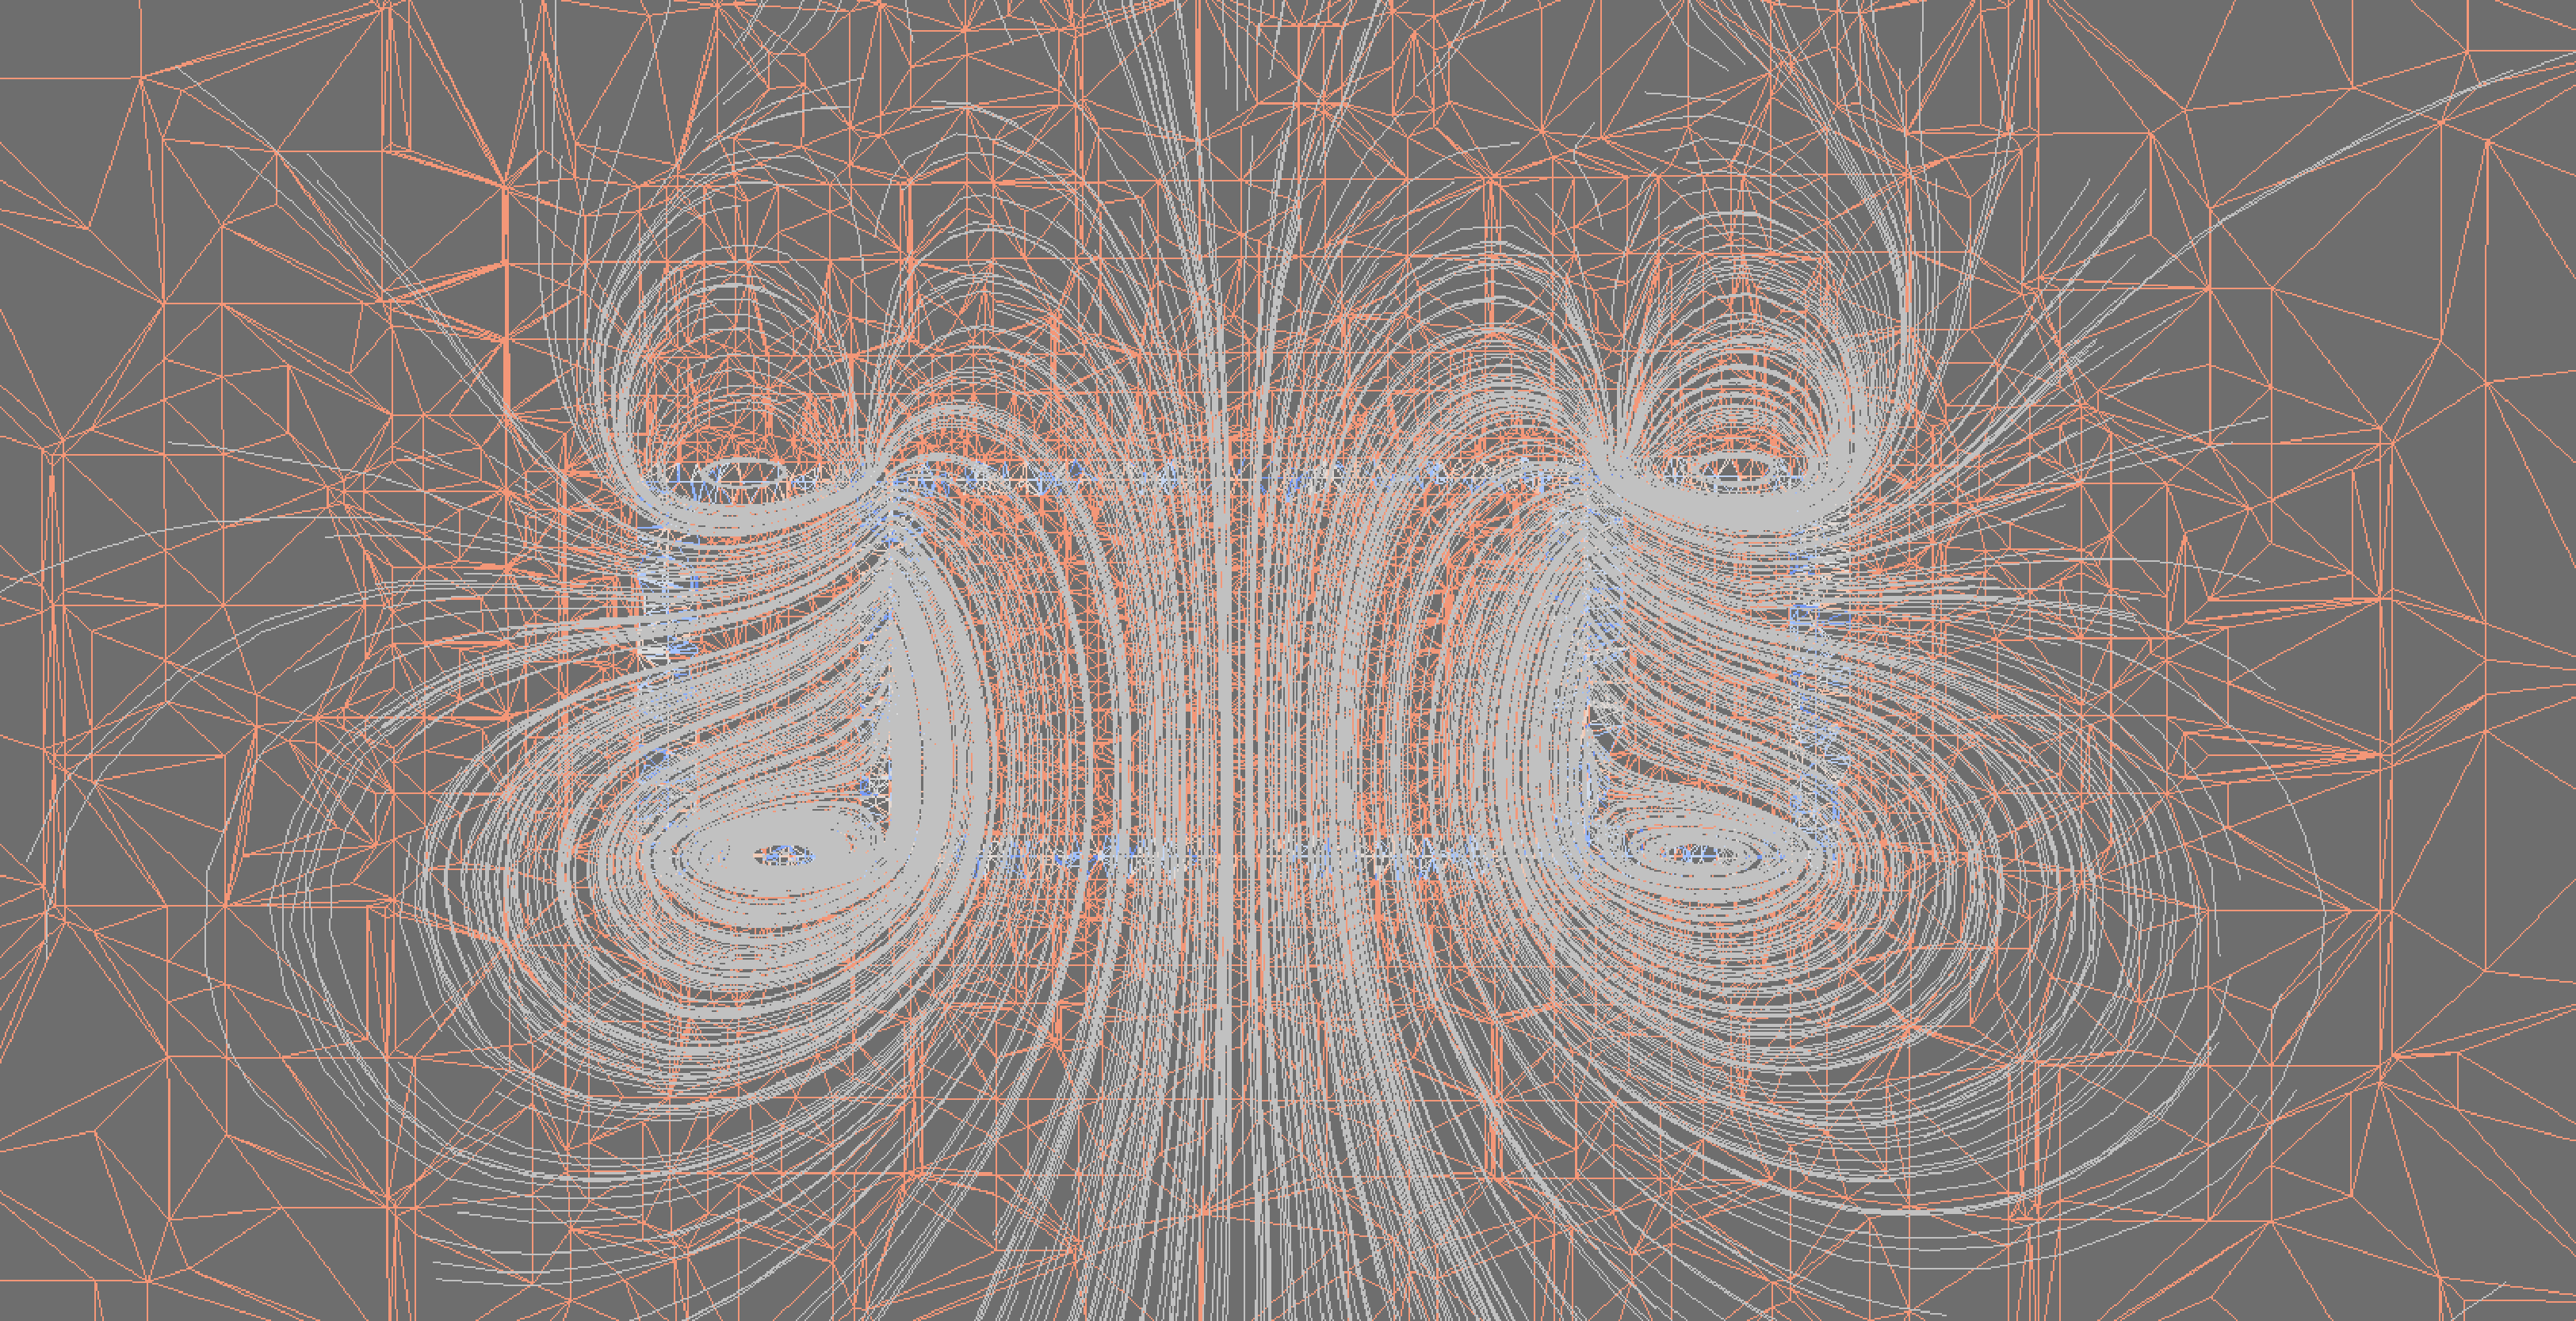
\includegraphics[width = .8\textwidth]{M4shellmagnet2}}
\end{figure}

\item[Coil] Unico elemento attivo dell'attuatore, è costituito da un solenoide multi-strato in rame le cui caratteristiche sono mostrate in Tabella~\ref{tab:M4coildata}.

\begin{figure}[htb]
\centering
\caption{Induzione magnetica generata dal solenoide}
\label{fig:M4coil}
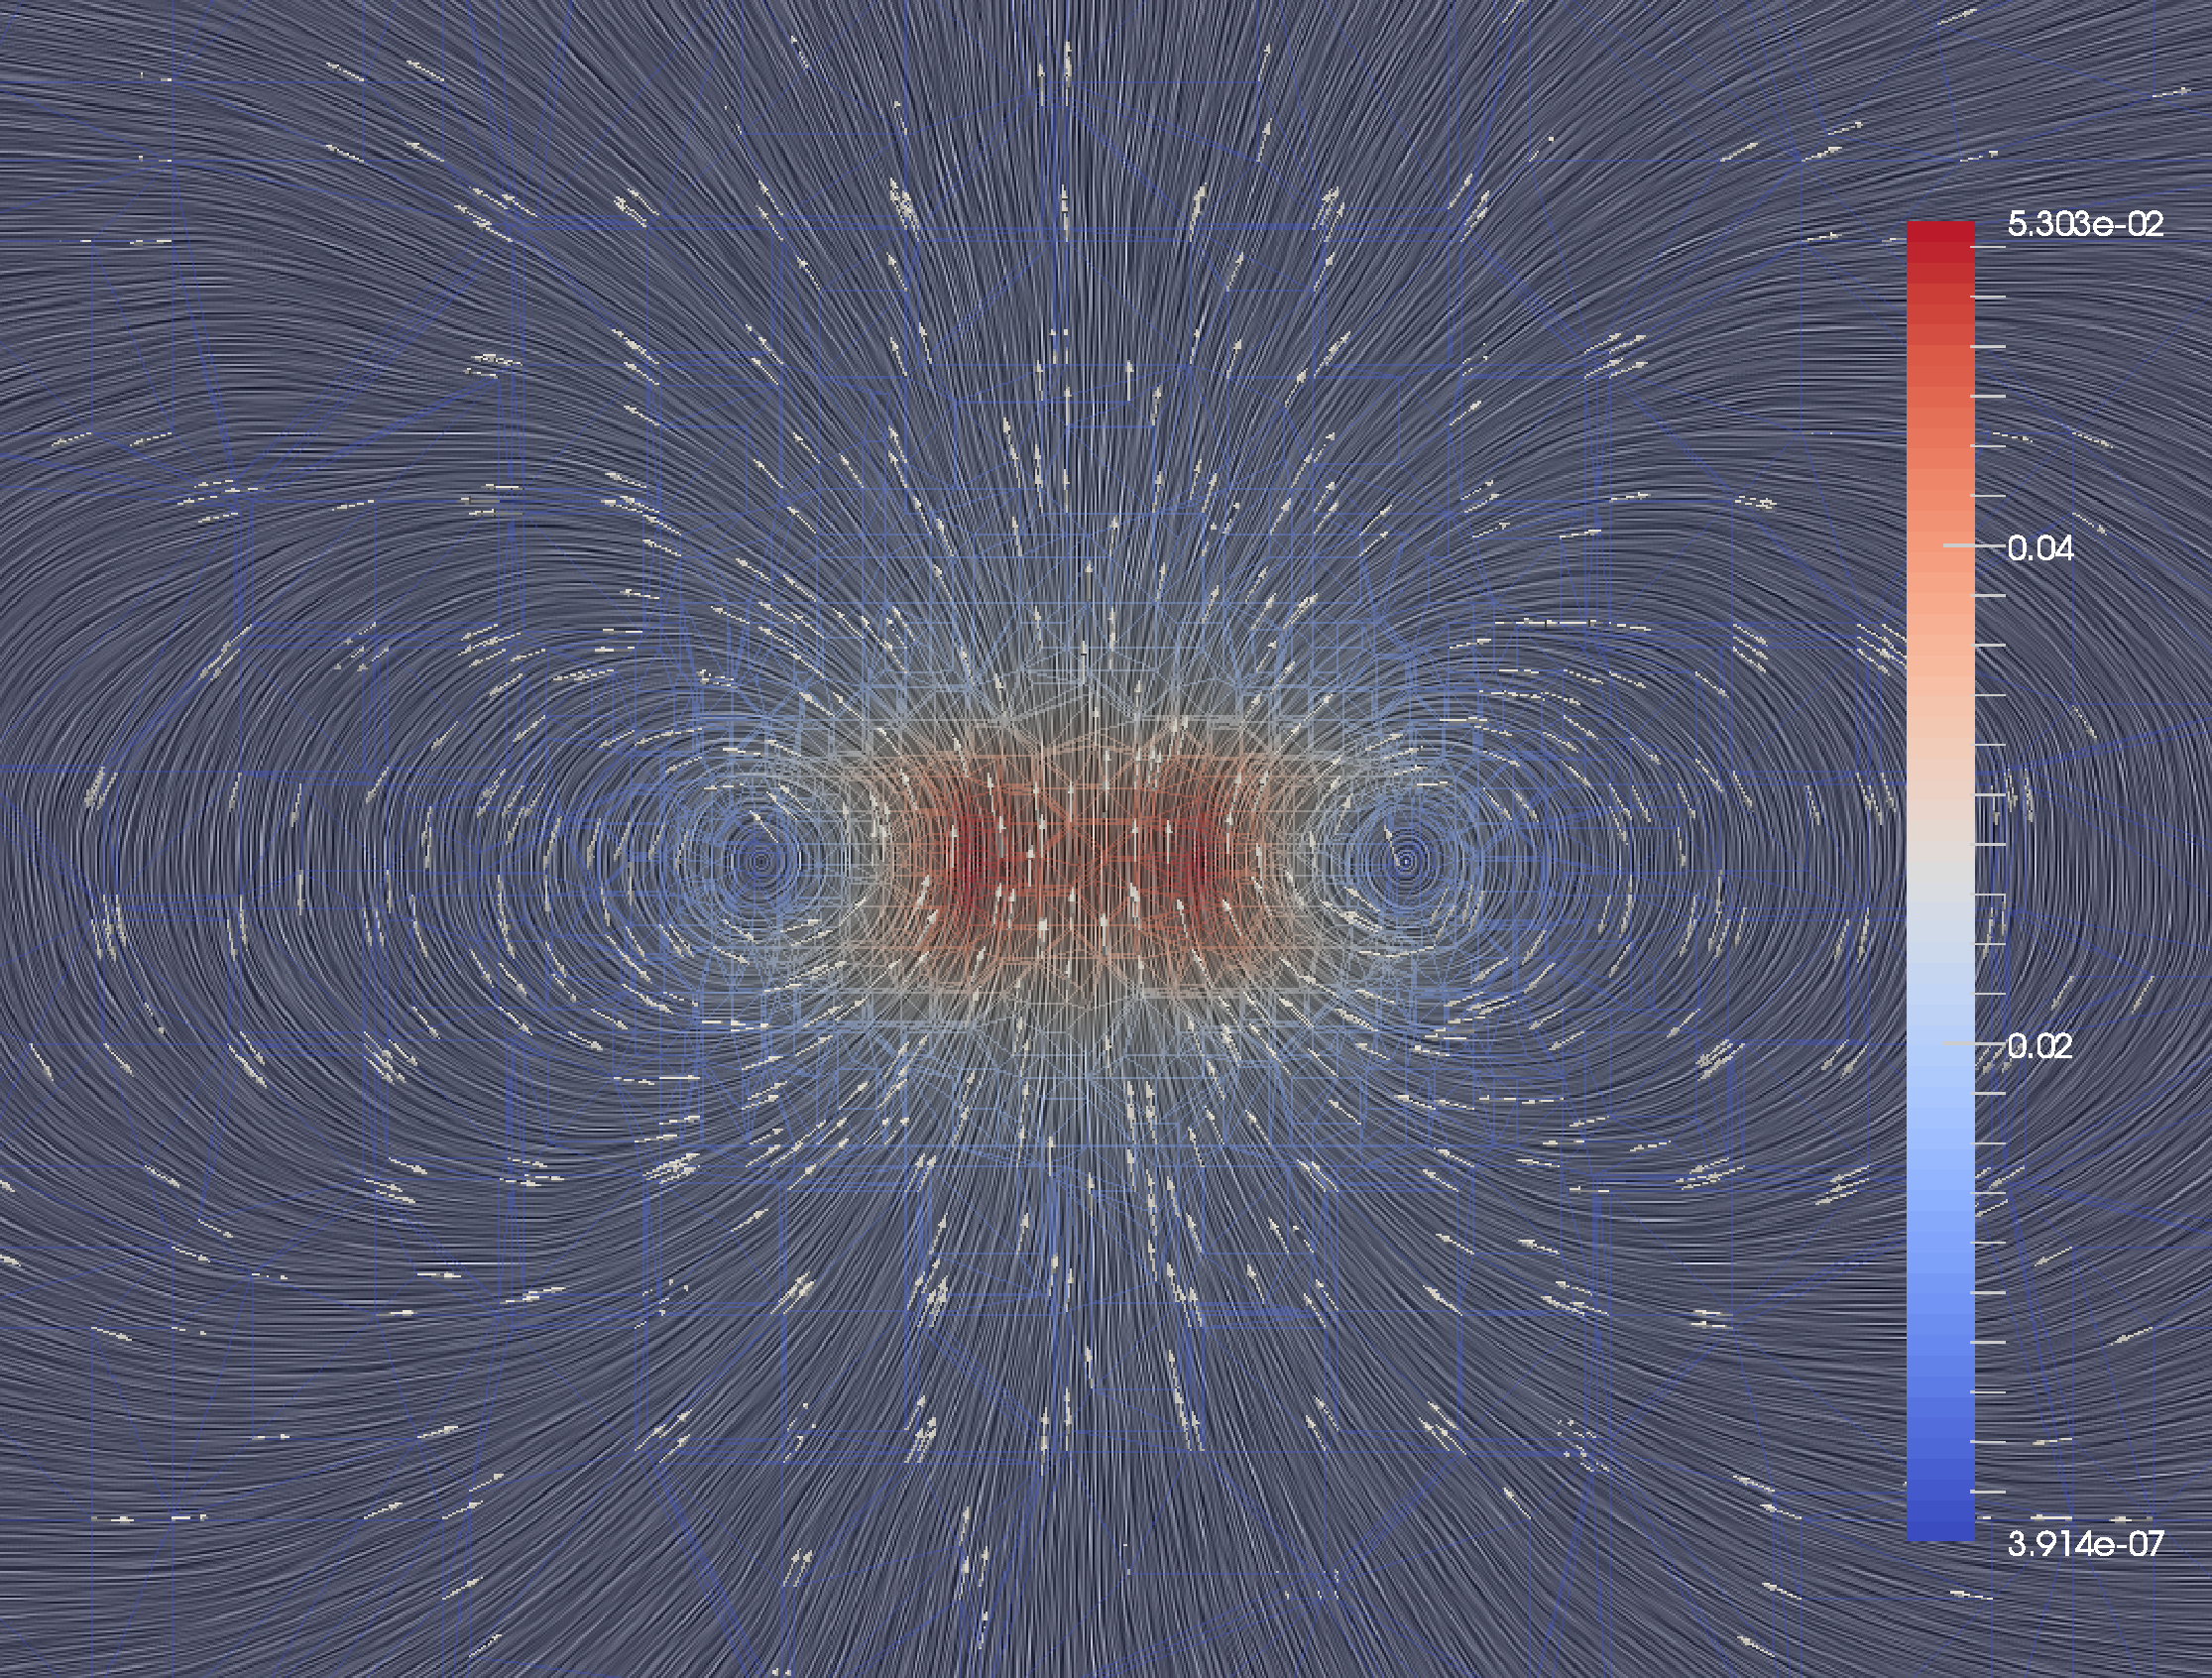
\includegraphics[width = .6\textwidth]{M4coil}
\end{figure}

Questo elemento è solidale al reference-body e posizionato al di sotto dello shell-magnet, ad una distanza di 0.2 mm \textit{face to face}. Il campo attorno all'induttore è mostrato in Figura \ref{fig:M4coil}.

\begin{SCtable}[1.][htb]
\centering
\footnotesize
\caption{Dati geometrici del solenoide}
\label{tab:M4coildata}
\begin{tabular}{l}
\toprule
\textit{Coil}\\
\midrule
\begin{tabular}{lc}
Raggio interno &  2.2 mm\\
Raggio esterno &  7 mm\\
Altezza &  3.2 mm\\
Numero di spire & 240\\
Materiale & Cu\\
\end{tabular}\\
\bottomrule
\end{tabular}
\end{SCtable}

\item[Bias-Magnet] Scopo di questo elemento è evitare il collasso del sistema se il sistema di controllo viene spento. Si tratta di un magnete tubolare in lega di neodimio-ferro-boro con induzione residua assiale di intensità $\T{b_r} = 1.17$ T. \'E solidale al reference-body e viene posizionato al di sotto dello shell-magnet e del coil in modo che le due magnetizzazioni residue siano parallele e concordi. La distanza \textit{face to face} tra il magnete di bias e quello sullo specchio è di 6.1 mm.

\begin{figure}[htb]
\centering
\caption{Induzione magnetica generata dal bias-magnet (sezione rispetto ad un diametro del magnete)}
\label{fig:M4biasmagnet}
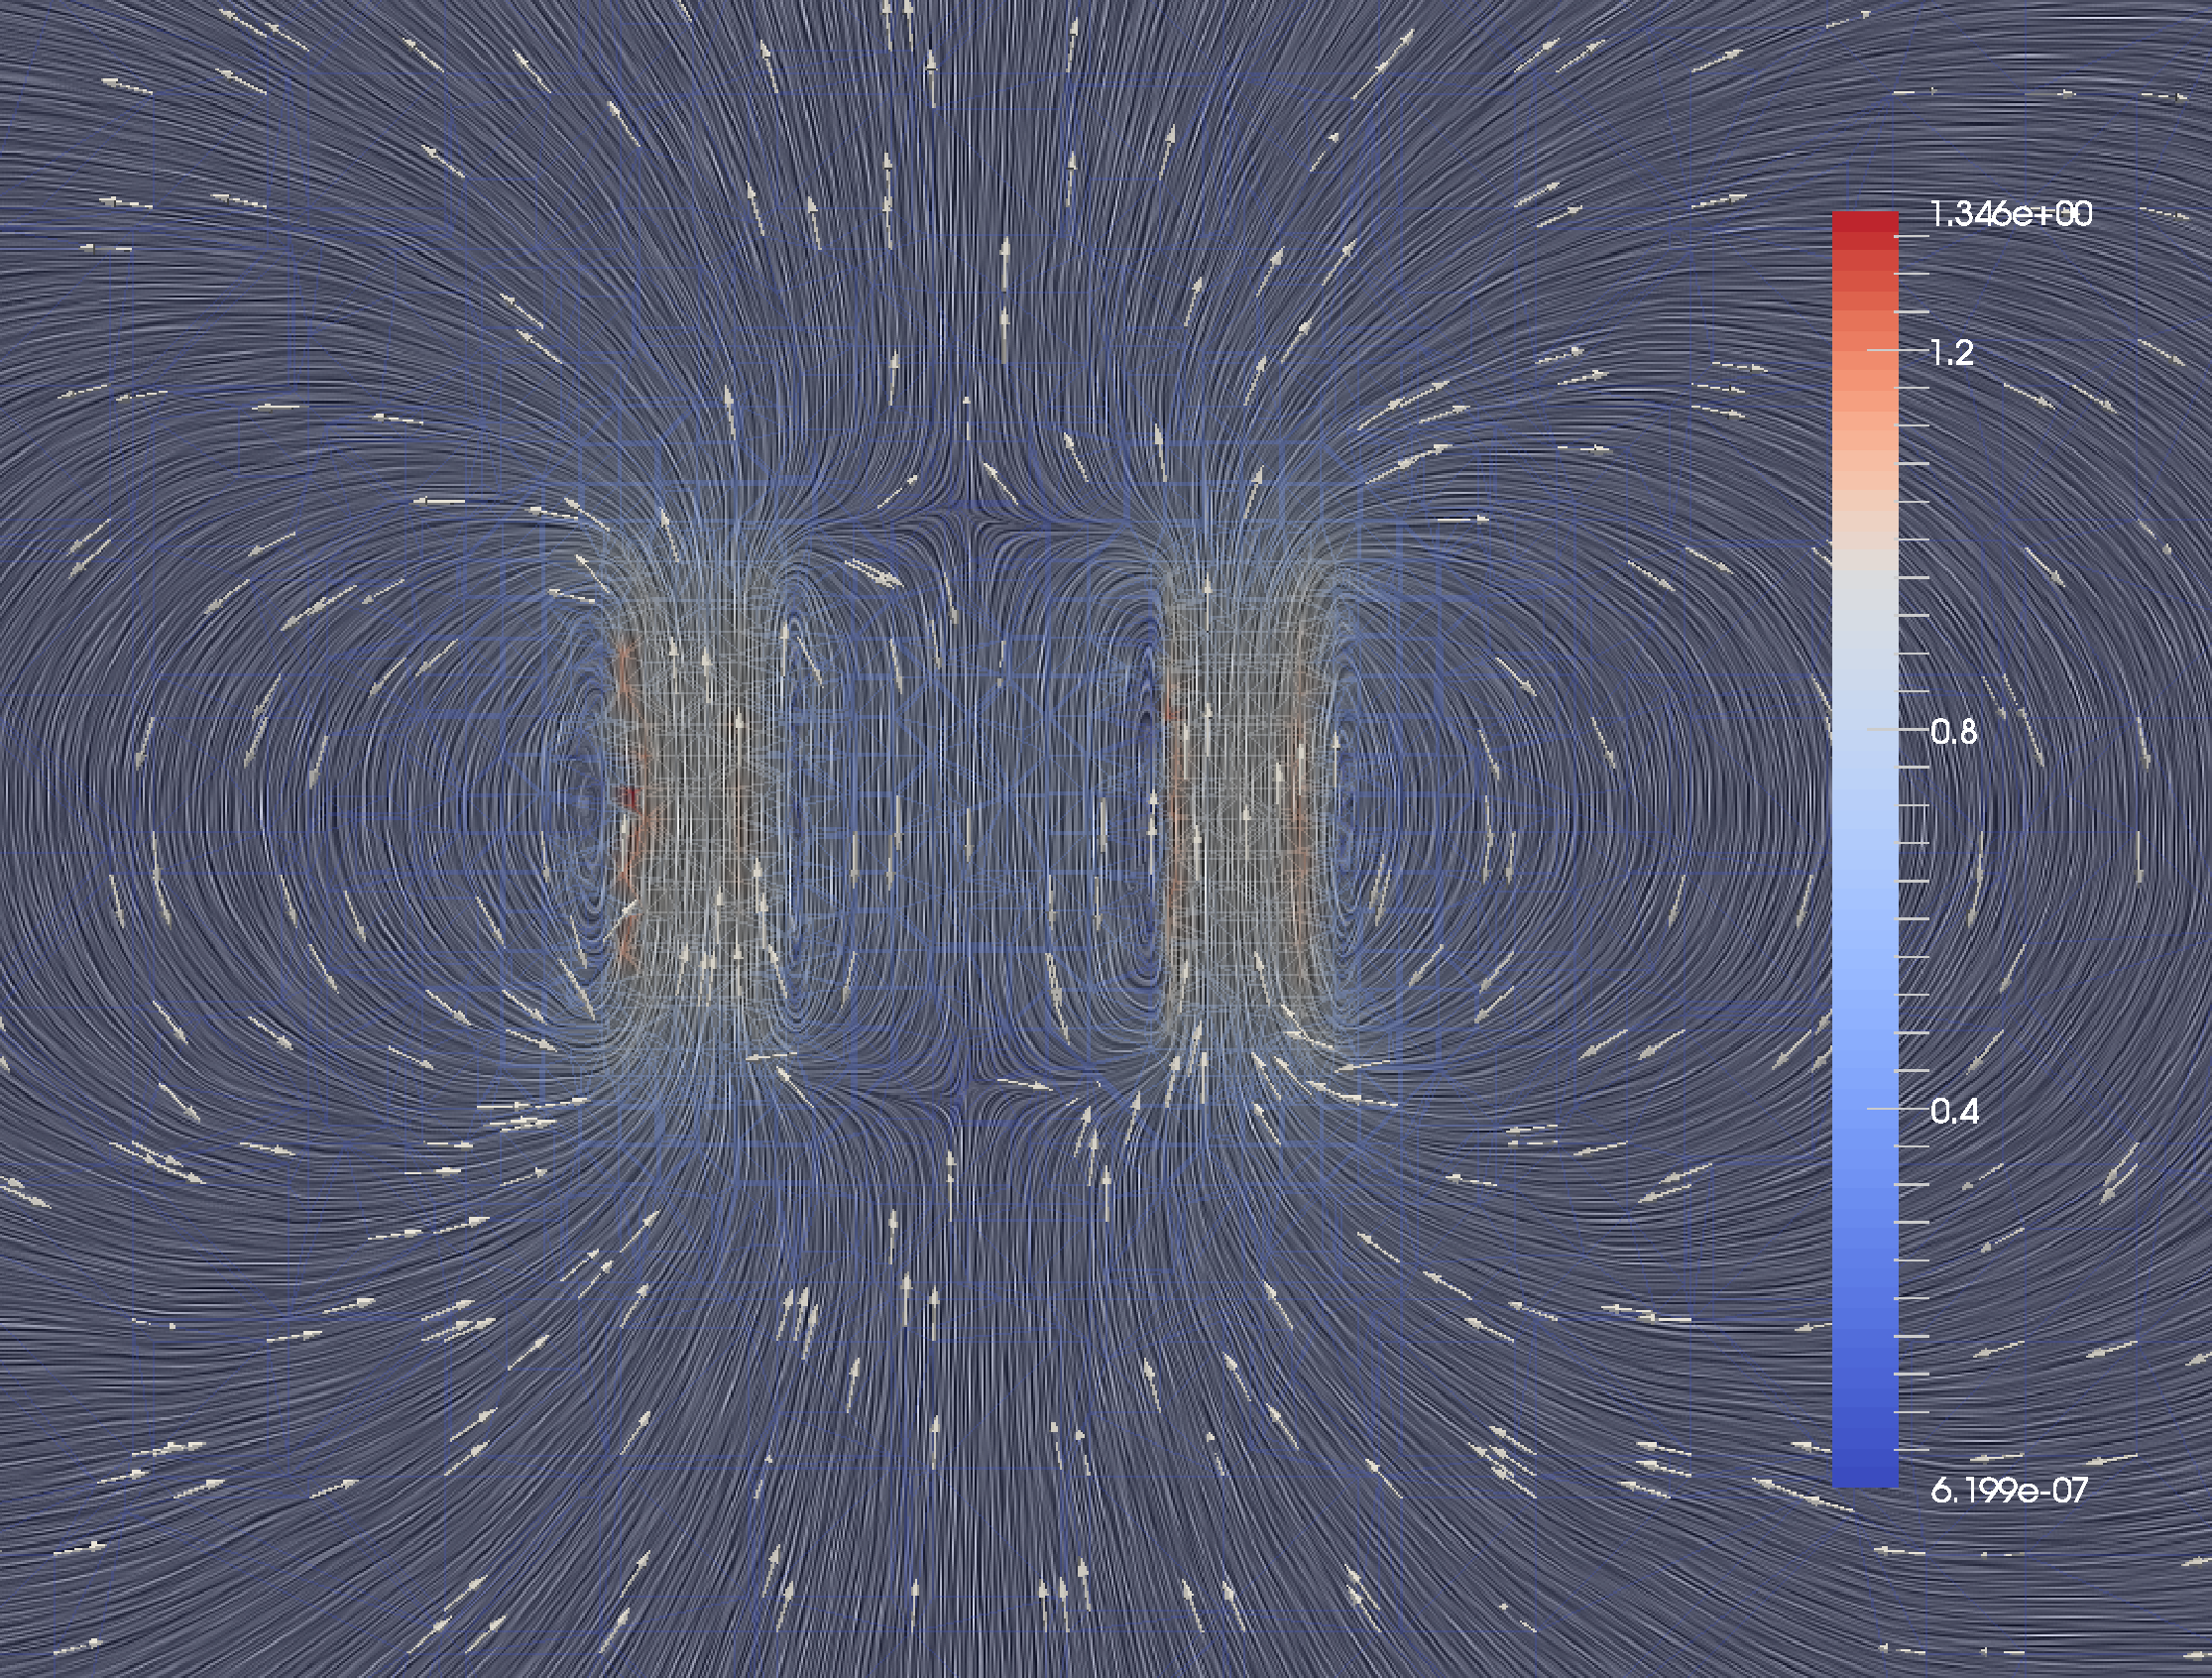
\includegraphics[width = .6\textwidth]{M4biasmagnet}
\end{figure}

I dati geometrici sul bias-magnet sono riportati in Tabella \ref{tab:M4biasmagnetdata} mentre il 
campo generato è mostrato in Figura \ref{fig:M4biasmagnet}.

\begin{SCtable}[1.][htb]
\centering
\footnotesize
\caption{Dati geometrici del magnete di bias}
\label{tab:M4biasmagnetdata}
\begin{tabular}{l}
\toprule
\textit{Bias}\\
\midrule
\begin{tabular}{lc}
Raggio interno &  0.75 mm\\
Raggio esterno &  1.5 mm\\
Altezza &  2 mm\\
Materiale & NdFeB N52\\
\end{tabular}\\
\bottomrule
\end{tabular}
\end{SCtable}
\end{description}

Come si può osservare, il campo magnetico del solenoide è completamente sovrastato da quello generato dai magneti permanenti. Infatti, anche per un valore di corrente $i = 10^6$ A l'induttore genera un campo magnetico $\T{b}$ dell'ordine di $10^{-2}$ T, mentre i magneti possiedono un campo dell'ordine di 1 T. 

Pertanto un'analisi in cui i campi di tutti gli elementi siano analizzati contemporaneamente comporta malcondizionamento della matrice assemblata e difficoltà nella convergenza della soluzione. Inoltre non è necessario il calcolo delle forze scambiate fra tutti gli elementi: dovendo calcolare la forza che agisce sul solenoide o sul magnete di bias, entrambi solidali al reference-body, solo il contributo del magnete solidale allo specchio è da considerare.

Le analisi saranno quindi condotte calcolando i contributi di forze e momenti considerando coppie di componenti, e sfruttando il principio della sovrapposizione degli effetti per ottenere le forze globali.

In questo modo una variazione di progetto sulla geometria o posizione di uno dei componenti non comporta la necessità di una nuova iterazione di tutte le analisi, ma solo di una sua parte.\\

I momenti sono stati calcolati rispetto al punto $P$ di intersezione fra l'asse dello shell magnet e il piano medio della piastra deformabile. In questo modo il momento ottenuto lavora direttamente per la rotazione del piano medio dello specchio. La distanza complessiva del polo dalla faccia superiore del magnete di shell è:
\begin{equation}
\label{eq:6polo}
d_P = t_{pot}+t_{puk}+\frac{t_{shell}}{2} = \left(0.2+2+\frac{1.95}{2}\right)\text{mm} = 3.175~\text{mm}.
\end{equation}
Nel caso in cui lo spessore della piastra o del puk varino, è necessario calcolare i contributi di trasporto sul nuovo polo.\\

Infine si riporta la struttura del sensore capacitivo: le due armature sono costituite da \textit{coating} aurei il cui spessore è circa 1$\mu$m. L'armatura solidale al reference-body è formata da una corona circolare e da uno svaso conico mentre l'altra è costituita dal rivestimento dello specchio stesso (Figura \ref{fig:m4condsection}). La distanza nominale fra le armature è di 90$\mu$m. Le caratteristiche della geometria del condensatore sono mostrate in Tabella \ref{tab:M4conddatageom}.

\begin{figure}[htb]
\centering
\caption{Sezione del sensore capacitivo}
\label{fig:m4condsection}
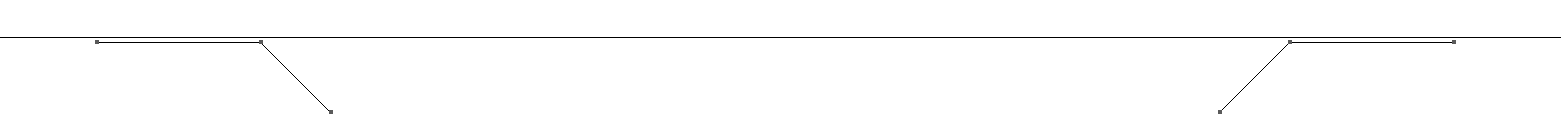
\includegraphics[width = \textwidth]{m4condsection}
\end{figure}

\begin{SCtable}[1.][htb]
\centering
\footnotesize
\caption{Dati geometrici del condensatore}
\label{tab:M4conddatageom}
\begin{tabular}{l}
\toprule
\begin{tabular}{lc}
Raggio interno &  14.5 mm\\
Raggio esterno &  11 mm\\
Distanza fra le armature &  90 $\mu$m\\
Ampiezza svaso & 1.5 mm\\
Altezza svaso & 1.5 mm\\
Materiale & Au\\
\end{tabular}\\
\bottomrule
\end{tabular}
\end{SCtable}

\section{Forze e coppie shell-magnet -- bias-magnet}
Una prima analisi riguarda il calcolo di forze e coppie scambiate tra i due magneti permanenti. Questi devono esercitare una forza sufficiente a garantire che, se il sistema di controllo viene spento, la piastra deformabile sia attratta verso il reference-body e vi resti unita stabilmente.

 La configurazione operativa prevede una distanza fra i due magneti di 6.1 mm, sufficiente ad effettuare il calcolo delle forze tramite il metodo della superficie di Maxwell. \'E stata svolta l'analisi per diverse forme e dimensioni. Una buona robustezza rispetto alle variabili di analisi (dimensione della mesh, dimensione della superficie, dimensione del dominio) è stata raggiunta utilizzando come superfici due calotte emisferiche di raggio $r_{Maxwell} = 15$ mm in modo che il piano che separa le due parti fosse equidistante dai due magneti.
Le caratteristiche del modello sono elencate in Tabella \ref{tab:M4shellbiasdata}. 

\begin{SCtable}[1.][htb]
\centering
\caption{Modello per il calcolo di forze tra i magneti di shell e di bias}
\label{tab:M4shellbiasdata}
\begin{tabular}{lc}
\toprule
Raggio dominio esterno &  60 mm\\
Raggio superficie di Maxwell &  15 mm\\
Numero di nodi &  235607\\
Numero di celle & 1398259\\
\bottomrule
\end{tabular}
\end{SCtable}

In Tabella \ref{tab:M4shellbiasforces1} sono mostrate le forze e coppie agenti sul magnete dello specchio per la configurazione nominale. Si può osservare che la forza è verticale e porta i due corpi ad avvicinarsi: le altre due componenti hanno valori che possono essere attribuiti a disomogeneità nella costruzione della griglia di calcolo. Risulta nullo anche il momento complessivo fra i due magneti. Sulla base dei risultati ottenuti si è scelto di considerare nulle forze al di sotto di 2 mN e coppie sotto la soglia di 0.02 N~mm. 
 

\begin{SCtable}[2.][htb]
\centering
\caption{Forze e coppie agenti sullo shell-magnet nella configurazione nominale}
\label{tab:M4shellbiasforces1}
\begin{tabular}{lc}
\toprule
$F_x$ & 0.15 mN\\
$F_y$ & 1.39 mN\\
$F_z$ & -250.74 mN\\
$M_x$ & 0.010 N~mm\\
$M_y$ & 0.009 N~mm\\
$M_z$ & 0.001 N~mm\\
\bottomrule
\end{tabular}
\end{SCtable}

Dopo aver ottenuto le forze e coppie per la configurazione nominale ne è stata valutata la sensibilità alla variazione di configurazione tramite il seguente ciclo:
\begin{itemize}
\item Variazione di un parametro tra distanza longitudinale, offset trasversale e angolo relativo (la rotazione è stata effettuata rispetto allo stesso polo usato per il calcolo dei momenti);
\item Rigenerazione della griglia di calcolo;
\item Soluzione del problema ed estrapolazione delle forze;
\end{itemize}

\'E stato valutato l'andamento rispetto alle seguenti variazioni della configurazione dello shell-magnet:
\begin{enumerate}
\item scostamento longitudinale: $dz = \left[-0.1,0.1\right]$ mm
\item offset trasversale: $dx = \left[-0.1,0.1\right]$ mm
\item rotazione rispetto al polo $P$: $\alpha_y = \left[-5,5\right]$°
\end{enumerate}

\begin{figure}
\footnotesize
\centering
\subfloat[][]{
 \begin{tikzpicture}
    \begin{axis}[axis y line = left,
                 grid = major,
                 axis x line = left,
    		     width = .4\textwidth,
    		     height = .15\textheight,
                 ylabel = {Forze (mN)}, 
                 xlabel = {Distanza verticale $z$ (mm)},
                 xmin = 6,
                 xmax = 6.25,
                 ymin = -5.,
                 ymax = 15]
    \addplot[mark = triangle*, samples = 200., smooth]
    file {./Immagini/ActSens/m4shellbiasfxz.dat};
    \addplot[mark = square*, samples = 200, smooth]
    file {./Immagini/ActSens/m4shellbiasfyz.dat};
    \legend{$f_x$\\$f_y$\\}
    \end{axis}
    \end{tikzpicture}
    }
\subfloat[][]{
 \begin{tikzpicture}
    \begin{axis}[axis y line = left,
                 grid = major,
                 axis x line = left,
    		     width = .4\textwidth,
    		     height = .15\textheight,
                 ylabel = {Forze (mN)}, 
                 xlabel = {Distanza verticale $z$ (mm)},
                 xmin = 6,
                 xmax = 6.25,
                 ymin = -300.,
                 ymax = -200]
        \addplot[mark = *, samples = 200, smooth]
    file {./Immagini/ActSens/m4shellbiasfzz.dat};
    \legend{$f_z$\\}
    \end{axis}
    \end{tikzpicture}
    }\\
\subfloat[][]{
 \begin{tikzpicture}
    \begin{axis}[axis y line = left,
                 axis x line = left,
                 grid = major,
    		     width = .8\textwidth,
    		     height = .15\textheight,
                 ylabel = {Momenti (N~mm)}, 
                 xlabel = {Distanza verticale $z$ (mm)},
				 xmin = 6,
				 xmax = 6.25,
                 ymin = -.02, 
                 ymax = .07]
    \addplot[mark = triangle*, samples = 200, smooth]
    file {./Immagini/ActSens/m4shellbiasmxz.dat};
    \addplot[mark = square*, samples = 200, smooth]
    file {./Immagini/ActSens/m4shellbiasmyz.dat};
    \addplot[mark = *, samples = 200, smooth]
    file {./Immagini/ActSens/m4shellbiasmzz.dat};
    \legend{$m_x$\\$m_y$\\$m_z$\\}
    \end{axis}
    \end{tikzpicture}
    }
\caption{Accoppiamento shell-bias: andamento di forze e coppie rispetto a $z$}
\label{fig:M4shellbiasplots1}
\end{figure}

\begin{figure}
\footnotesize
\centering
\subfloat[][]{
 \begin{tikzpicture}
    \begin{axis}[axis y line = left,
                 grid = major,
                 axis x line = left,
    		     width = .4\textwidth,
    		     height = .15\textheight,
                 ylabel = {Forze (mN)}, 
                 xlabel = {Offset orizzontale $dx$ (mm)},
                 xmin = -.1,
                 xmax = .15,
                 ymin = -5.,
                 ymax = 15]
    \addplot[mark = triangle*, samples = 200., smooth]
    file {./Immagini/ActSens/m4shellbiasfxx.dat};
    \addplot[mark = square*, samples = 200, smooth]
    file {./Immagini/ActSens/m4shellbiasfyx.dat};
    \legend{$f_x$\\$f_y$\\}
    \end{axis}
    \end{tikzpicture}
    }
\subfloat[][]{
 \begin{tikzpicture}
    \begin{axis}[axis y line = left,
                 grid = major,
                 axis x line = left,
    		     width = .4\textwidth,
    		     height = .15\textheight,
                 ylabel = {Forze (mN)}, 
                 xlabel = {Offset orizzontale $dx$ (mm)},
                 xmin = -.1,
                 xmax = .15,
                 ymin = -260.,
                 ymax = -240]
        \addplot[mark = *, samples = 200, smooth]
    file {./Immagini/ActSens/m4shellbiasfzx.dat};
    \legend{$f_z$\\}
    \end{axis}
    \end{tikzpicture}
    }\\
\subfloat[][]{
 \begin{tikzpicture}
    \begin{axis}[axis y line = left,
                 axis x line = left,
                 legend pos=south east,
                 grid = major,
    		     width = .8\textwidth,
    		     height = .15\textheight,
                 ylabel = {Momenti (N~mm)}, 
                 xlabel = {Offset orizzontale $dx$ (mm)},
				 xmin = -.1,
				 xmax = .15,
                 ymin = -.15, 
                 ymax = .05]
    \addplot[mark = triangle*, samples = 200, smooth]
    file {./Immagini/ActSens/m4shellbiasmxx.dat};
    \addplot[mark = square*, samples = 200, smooth]
    file {./Immagini/ActSens/m4shellbiasmyx.dat};
    \addplot[mark = *, samples = 200, smooth]
    file {./Immagini/ActSens/m4shellbiasmzx.dat};
    \legend{$m_x$\\$m_y$\\$m_z$\\}
    \end{axis}
    \end{tikzpicture}
    }
\caption{Accoppiamento shell-bias: andamento di forze e coppie rispetto a $x$}
\label{fig:M4shellbiasplots2}
\end{figure}


\begin{figure}
\footnotesize
\centering
\subfloat[][]{
 \begin{tikzpicture}
    \begin{axis}[axis y line = left,
                 grid = major,
                 axis x line = left,
    		     width = .4\textwidth,
    		     height = .15\textheight,
                 ylabel = {Forze (mN)}, 
                 xlabel = {Angolo $\alpha_y$ (°)},
                 xmin = -6,
                 xmax = 6.5,
                 ymin = -10.,
                 ymax = 20]
    \addplot[mark = triangle*, samples = 200., smooth]
    file {./Immagini/ActSens/m4shellbiasfxa.dat};
    \addplot[mark = square*, samples = 200, smooth]
    file {./Immagini/ActSens/m4shellbiasfya.dat};
    \legend{$f_x$\\$f_y$\\}
    \end{axis}
    \end{tikzpicture}
    }
\subfloat[][]{
 \begin{tikzpicture}
    \begin{axis}[axis y line = left,
                 grid = major,
                 axis x line = left,
    		     width = .4\textwidth,
    		     height = .15\textheight,
                 ylabel = {Forze (mN)}, 
                 xlabel = {Angolo $\alpha_y$ (°)},
                 xmin = -6,
                 xmax = 6.5,
                 ymin = -260.,
                 ymax = -200]
        \addplot[mark = *, samples = 200, smooth]
    file {./Immagini/ActSens/m4shellbiasfza.dat};
    \legend{$f_z$\\}
    \end{axis}
    \end{tikzpicture}
    }\\
\subfloat[][]{
 \begin{tikzpicture}
    \begin{axis}[axis y line = left,
                 axis x line = left,
                 grid = major,
    		     width = .8\textwidth,
    		     height = .15\textheight,
                 ylabel = {Momenti (N~mm)}, 
                 xlabel = {Angolo $\alpha_y$ (°)},
				 xmin = -6,
				 xmax = 6.5,
                 ymin = -.05, 
                 ymax = .15]
    \addplot[mark = triangle*, samples = 200, smooth]
    file {./Immagini/ActSens/m4shellbiasmxa.dat};
    \addplot[mark = square*, samples = 200, smooth]
    file {./Immagini/ActSens/m4shellbiasmya.dat};
    \addplot[mark = *, samples = 200, smooth]
    file {./Immagini/ActSens/m4shellbiasmza.dat};
    \legend{$m_x$\\$m_y$\\$m_z$\\}
    \end{axis}
    \end{tikzpicture}
    }
\caption{Accoppiamento shell-bias: andamento di forze e coppie rispetto a $\theta_y$}
\label{fig:M4shellbiasplots3}
\end{figure}

Nelle Figure \ref{fig:M4shellbiasplots1}--\ref{fig:M4shellbiasplots3} sono mostrati i risultati ottenuti per le configurazioni considerate. Osservando i grafici si può osservare l'andamento delle forze e se ne può estrapolare la pendenza rispetto alla configurazione di riferimento.

Approssimando come serie di Taylor al primo ordine le forze e coppie in funzione degli scostamenti e angoli di rotazione si può scrivere:
\begin{equation}
\label{eq:6fc_xzalfa}
\begin{array}{cc}
\T{f} = 
\left\{\begin{array}{c}
F_x\\
F_y\\
F_z\\
C_x\\
C_y\\
C_z\end{array}\right\}
&
\T{x} = 
\left\{\begin{array}{c}
x\\
y\\
z\\
\alpha_x\\
\alpha_y\\
\alpha_z\end{array}\right\}
\end{array}
\end{equation}
\begin{equation}
\label{eq:6fc_xzalfa2}
\T{f} = \T{f_0}+\TT{E}\T{x},
\end{equation}
dove:
\begin{equation}
\label{eq:6fc_xzalfa3}
\TT{E} = \left[
\de_x\T{f}~|~\de_y\T{f}~|~\de_z\T{f}~|~ \de_{\alpha_x}\T{f}~|~\de_{\alpha_y}\T{f}~|~\de_{\alpha_z}\T{f}\right].
\end{equation}

Dalle analisi effettuate, considerando la simmetria assiale, si possono estrapolare i seguenti dati:
\begin{equation}
\label{eq:6fc_xzalfa5}
\nonumber
\footnotesize
\begin{array}{c}
\T{f_0} = 
\left\{\begin{array}{c}
0~\text{mN}\\
0~\text{mN}\\
-250~\text{mN}\\
0~\text{Nmm}\\
0~\text{Nmm}\\
0~\text{Nmm}
\end{array}\right\}
\\~\\
\TT{E} = 
\left[\begin{array}{cccccc}
-48.6~\frac{\text{mN}}{\text{mm}} &
0~\frac{\text{mN}}{\text{mm}} &
0~\frac{\text{mN}}{\text{mm}} &
0~\frac{\text{mN}}{\text{rad}} &
-76.9~\frac{\text{mN}}{\text{rad}} &
0~\frac{\text{mN}}{\text{rad}}\\

0~\frac{\text{mN}}{\text{mm}} &
-48.6~\frac{\text{mN}}{\text{mm}} &
0~\frac{\text{mN}}{\text{mm}} &
76.9~\frac{\text{mN}}{\text{rad}} &
0~\frac{\text{mN}}{\text{rad}} &
0~\frac{\text{mN}}{\text{rad}}\\


0~\frac{\text{mN}}{\text{mm}} &
0~\frac{\text{mN}}{\text{mm}} &
87.4~\frac{\text{mN}}{\text{mm}} &
0~\frac{\text{mN}}{\text{rad}} &
0~\frac{\text{mN}}{\text{rad}} &
0~\frac{\text{mN}}{\text{rad}}\\

0~\text{N} &
-0.27~\text{N} &
0~\text{N} &
-0.07~\frac{\text{Nmm}}{\text{rad}} &
0~\frac{\text{Nmm}}{\text{rad}} &
0~\frac{\text{Nmm}}{\text{rad}}\\

0.27~\text{N} &
0~\text{N} &
0~\text{N} &
0~\frac{\text{Nmm}}{\text{rad}} &
-0.07~\frac{\text{Nmm}}{\text{rad}} &
0~\frac{\text{Nmm}}{\text{rad}}\\

0~\text{N} &
0~\text{N} &
0~\text{N} &
0~\frac{\text{Nmm}}{\text{rad}} &
0~\frac{\text{Nmm}}{\text{rad}} &
0~\frac{\text{Nmm}}{\text{rad}}
\end{array}\right]

\end{array}
\end{equation}

Si può osservare la natura quasi diagonale della matrice, con i soli accoppiamenti non trascurabili dovuti all'interazione fra traslazioni laterali e rotazioni. Tale interazione è dovuta in parte proprio alla scelta del polo, poiché una rotazione infinitesima $d\theta_y$ comporta un movimento $dx$ secondo la direzione della rotazione. Nelle analisi strutturali successive verrà trascurato il moto laterale dello specchio, in quanto disaccoppiato e di entità ampiamente trascurabile. Gli effetti delle tolleranze di assemblaggio e degli scorrimenti laterali dovuti alla gravità verranno modellati attraverso una distribuzione di \textit{offset} laterali opportunamente generata. L'introduzione di questo particolare effetto porterà ad un accoppiamento non trascurabile tra gradi di libertà della piastra.

Si nota dai termini diagonali che il contributo del magnete di bias è stabilizzante per tutti i gradi di libertà eccezion fatta per lo spostamento trasversale, in cui è garantita l'adesione tra lo specchio e il reference-body in caso di spegnimento del sistema di controllo se la forza $F_{z_0}$ moltiplicata per il numero di attuatori è maggiore del peso complessivo dello specchio strumentato.

\section{Forze e coppie shell-magnet -- coil}
\label{sec:shellcoilforces}
Si prosegue analizzando forze e coppie scambiate tra il magnete solidale allo specchio e il solenoide. Per il calcolo è stato utilizzata la formula di Lorentz, attivando il campo del magnete permanente e integrando la quantità $\T{f_L} = \T{b}\times\T{j}$ nel volume occupato dal solenoide. Per l'analisi si è considerata $j$ positiva in senso antiorario. Le forze sono calcolate per $i  = 1$ A, e rappresentano i coefficienti $K_m$, costanti di proporzionalità tra corrente impressa e forze generate dall'attuatore.\\

La configurazione operativa prevede una distanza fra i due magneti di 0.2 mm, distanza che non ha permesso l'utilizzo del metodo della superficie di Maxwell e che ha limitato l'escursione angolare relativa dei due elementi a $0.8$°. 
Le caratteristiche del modello sono elencate in Tabella \ref{tab:M4shellcoildata}. 

\begin{SCtable}[1.][htb]
\centering
\caption{Modello preparato per il calcolo di forze tra il magnete di shell e il solenoide}
\label{tab:M4shellcoildata}
\begin{tabular}{lc}
\toprule
Raggio dominio esterno &  100 mm\\
Numero di nodi &  224207\\
Numero di celle & 1330900\\
\bottomrule
\end{tabular}
\end{SCtable}

In Tabella \ref{tab:M4shellcoilforces1} sono mostrate le forze e coppie agenti sul magnete dello specchio per la configurazione nominale. Si può osservare che anche in questo caso la forza è interamente verticale, e che la precisione raggiunta è molto maggiore (ove possibile, infatti, è sempre consigliabile calcolare le forze utilizzando direttamente la formula di Lorentz).

Anche in questo caso è stata verificata la stabilità del risultato ottenuto rispetto a variazioni di dimensione del dominio di calcolo e dimensione degli elementi.

\begin{SCtable}[2.][htb]
\centering
\caption{Forze e coppie agenti sul coil nella configurazione nominale}
\label{tab:M4shellcoilforces1}
\begin{tabular}{lc}
\toprule
$F_x$ & -0.04 mN\\
$F_y$ & -0.03 mN\\
$F_z$ & -1945.62 mN\\
$M_x$ & 0.00 N~mm\\
$M_y$ & 0.00 N~mm\\
$M_z$ & 0.00 N~mm\\
\bottomrule
\end{tabular}
\end{SCtable}

\'E stato valutato l'andamento rispetto alle seguenti variazioni della configurazione dello shell-magnet:
\begin{enumerate}
\item scostamento longitudinale: $dz = \left[-0.1,0.1\right]$ mm
\item offset trasversale: $dx = \left[-0.1,0.1\right]$ mm
\item rotazione rispetto al polo $P$: $\alpha_y = \left[-0.8,0.8\right]$°
\end{enumerate}


\begin{figure}
\footnotesize
\centering
\subfloat[][]{
 \begin{tikzpicture}
    \begin{axis}[axis y line = left,
                 grid = major,
                 axis x line = left,
    		     width = .4\textwidth,
    		     height = .15\textheight,
                 ylabel = {Forze (mN)}, 
                 xlabel = {Distanza verticale $z$ (mm)},
                 xmin = .1,
                 xmax = .35,
                 ymin = -3.,
                 ymax = 5]
    \addplot[mark = triangle*, samples = 200., smooth]
    file {./Immagini/ActSens/m4shellcoilfxz.dat};
    \addplot[mark = square*, samples = 200, smooth]
    file {./Immagini/ActSens/m4shellcoilfyz.dat};
    \legend{$f_x$\\$f_y$\\}
    \end{axis}
    \end{tikzpicture}
    }
\subfloat[][]{
 \begin{tikzpicture}
    \begin{axis}[axis y line = left,
                 grid = major,
                 axis x line = left,
                 legend pos=south east,
    		     width = .4\textwidth,
    		     height = .15\textheight,
                 ylabel = {Forze (mN)}, 
                 xlabel = {Distanza verticale $z$ (mm)},
                 xmin = .1,
                 xmax = .35,
                 ymin = -2100.,
                 ymax = -1800]
        \addplot[mark = *, samples = 200, smooth]
    file {./Immagini/ActSens/m4shellcoilfzz.dat};
    \legend{$f_z$\\}
    \end{axis}
    \end{tikzpicture}
    }\\
\subfloat[][]{
 \begin{tikzpicture}
    \begin{axis}[axis y line = left,
                 axis x line = left,
                 grid = major,
    		     width = .8\textwidth,
    		     height = .15\textheight,
                 ylabel = {Momenti (N~mm)}, 
                 xlabel = {Distanza verticale $z$ (mm)},
				 xmin = .1,
				 xmax = .35,
                 ymin = -.03, 
                 ymax = .06]
    \addplot[mark = triangle*, samples = 200, smooth]
    file {./Immagini/ActSens/m4shellcoilmxz.dat};
    \addplot[mark = square*, samples = 200, smooth]
    file {./Immagini/ActSens/m4shellcoilmyz.dat};
    \addplot[mark = *, samples = 200, smooth]
    file {./Immagini/ActSens/m4shellcoilmzz.dat};
    \legend{$m_x$\\$m_y$\\$m_z$\\}
    \end{axis}
    \end{tikzpicture}
    }
\caption{Accoppiamento shell-coil: andamento di forze e coppie rispetto a $z$}
\label{fig:M4shellcoilplots1}
\end{figure}

\begin{figure}
\footnotesize
\centering
\subfloat[][]{
 \begin{tikzpicture}
    \begin{axis}[axis y line = left,
                 grid = major,
                 axis x line = left,
    		     width = .4\textwidth,
    		     height = .15\textheight,
                 ylabel = {Forze (mN)}, 
                 xlabel = {Offset orizzontale $dx$ (mm)},
                 xmin = -.1,
                 xmax = .15,
                 ymin = -40,
                 ymax = 60]
    \addplot[mark = triangle*, samples = 200., smooth]
    file {./Immagini/ActSens/m4shellcoilfxx.dat};
    \addplot[mark = square*, samples = 200, smooth]
    file {./Immagini/ActSens/m4shellcoilfyx.dat};
    \legend{$f_x$\\$f_y$\\}
    \end{axis}
    \end{tikzpicture}
    }
\subfloat[][]{
 \begin{tikzpicture}
    \begin{axis}[axis y line = left,
                 grid = major,
                 axis x line = left,
    		     width = .4\textwidth,
    		     height = .15\textheight,
                 ylabel = {Forze (mN)}, 
                 xlabel = {Offset orizzontale $dx$ (mm)},
                 xmin = -.1,
                 xmax = .15,
                 ymin = -2000.,
                 ymax = -1900]
        \addplot[mark = *, samples = 200, smooth]
    file {./Immagini/ActSens/m4shellcoilfzx.dat};
    \legend{$f_z$\\}
    \end{axis}
    \end{tikzpicture}
    }\\
\subfloat[][]{
 \begin{tikzpicture}
    \begin{axis}[axis y line = left,
                 axis x line = left,
                 legend pos=south east,
                 grid = major,
    		     width = .8\textwidth,
    		     height = .15\textheight,
                 ylabel = {Momenti (N~mm)}, 
                 xlabel = {Offset orizzontale $dx$ (mm)},
				 xmin = -.1,
				 xmax = .15,
                 ymin = -.6, 
                 ymax = .4]
    \addplot[mark = triangle*, samples = 200, smooth]
    file {./Immagini/ActSens/m4shellcoilmxx.dat};
    \addplot[mark = square*, samples = 200, smooth]
    file {./Immagini/ActSens/m4shellcoilmyx.dat};
    \addplot[mark = *, samples = 200, smooth]
    file {./Immagini/ActSens/m4shellcoilmzx.dat};
    \legend{$m_x$\\$m_y$\\$m_z$\\}
    \end{axis}
    \end{tikzpicture}
    }
\caption{Accoppiamento shell-coil: andamento di forze e coppie rispetto a $x$}
\label{fig:M4shellcoilplots2}
\end{figure}


\begin{figure}
\footnotesize
\centering
\subfloat[][]{
 \begin{tikzpicture}
    \begin{axis}[axis y line = left,
                 grid = major,
                 axis x line = left,
    		     width = .4\textwidth,
    		     height = .15\textheight,
                 ylabel = {Forze (mN)}, 
                 xlabel = {Angolo $\alpha_y$ (°)},
                 xmin = -.8,
                 xmax = 1,
                 ymin = -7.,
                 ymax = 13]
    \addplot[mark = triangle*, samples = 200., smooth]
    file {./Immagini/ActSens/m4shellcoilfxa.dat};
    \addplot[mark = square*, samples = 200, smooth]
    file {./Immagini/ActSens/m4shellcoilfya.dat};
    \legend{$f_x$\\$f_y$\\}
    \end{axis}
    \end{tikzpicture}
    }
\subfloat[][]{
 \begin{tikzpicture}
    \begin{axis}[axis y line = left,
                 grid = major,
                 axis x line = left,
    		     width = .4\textwidth,
    		     height = .15\textheight,
                 ylabel = {Forze (mN)}, 
                 xlabel = {Angolo $\alpha_y$ (°)},
                 xmin = -.8,
                 xmax = 1,
                 ymin = -2000.,
                 ymax = -1900]
        \addplot[mark = *, samples = 200, smooth]
    file {./Immagini/ActSens/m4shellcoilfza.dat};
    \legend{$f_z$\\}
    \end{axis}
    \end{tikzpicture}
    }\\
\subfloat[][]{
 \begin{tikzpicture}
    \begin{axis}[axis y line = left,
                 axis x line = left,
                 grid = major,
    		     width = .8\textwidth,
    		     height = .15\textheight,
                 ylabel = {Momenti (N~mm)}, 
                 xlabel = {Angolo $\alpha_y$ (°)},
				 xmin = -.8,
				 xmax = 1,
                 ymin = -.02, 
                 ymax = .06]
    \addplot[mark = triangle*, samples = 200, smooth]
    file {./Immagini/ActSens/m4shellcoilmxa.dat};
    \addplot[mark = square*, samples = 200, smooth]
    file {./Immagini/ActSens/m4shellcoilmya.dat};
    \addplot[ mark = *, samples = 200, smooth]
    file {./Immagini/ActSens/m4shellcoilmza.dat};
    \legend{$m_x$\\$m_y$\\$m_z$\\}
    \end{axis}
    \end{tikzpicture}
    }
\caption{Accoppiamento shell-coil: andamento di forze e coppie rispetto a $\theta_y$}
\label{fig:M4shellcoilplots3}
\end{figure}

Nelle Figure \ref{fig:M4shellcoilplots1}--\ref{fig:M4shellcoilplots3} sono mostrati i risultati ottenuti.
Dalle elaborazioni sui dati riportati si ottiene:
\begin{equation}
\label{eq:6fc_xzalfa6}
\nonumber
\footnotesize
\begin{array}{c}
\T{f_0} = 
\left\{\begin{array}{c}
0~\text{mN}\\
0~\text{mN}\\
-1945.6~\text{mN}\\
0~\text{Nmm}\\
0~\text{Nmm}\\
0~\text{Nmm}
\end{array}\right\}
\\~\\
\TT{E} = 
\left[\begin{array}{cccccc}
-261.2~\frac{\text{mN}}{\text{mm}} &
0~\frac{\text{mN}}{\text{mm}} &
0~\frac{\text{mN}}{\text{mm}} &
0~\frac{\text{mN}}{\text{rad}} &
-367.7~\frac{\text{mN}}{\text{rad}} &
0~\frac{\text{mN}}{\text{rad}}\\

0~\frac{\text{mN}}{\text{mm}} &
-261.2~\frac{\text{mN}}{\text{mm}} &
0~\frac{\text{mN}}{\text{mm}} &
367.7~\frac{\text{mN}}{\text{rad}} &
0~\frac{\text{mN}}{\text{rad}} &
0~\frac{\text{mN}}{\text{rad}}\\


0~\frac{\text{mN}}{\text{mm}} &
0~\frac{\text{mN}}{\text{mm}} &
822.4~\frac{\text{mN}}{\text{mm}} &
0~\frac{\text{mN}}{\text{rad}} &
0~\frac{\text{mN}}{\text{rad}} &
0~\frac{\text{mN}}{\text{rad}}\\

0~\text{N} &
-1.39~\text{N} &
0~\text{N} &
-0.597~\frac{\text{Nmm}}{\text{rad}} &
0~\frac{\text{Nmm}}{\text{rad}} &
0~\frac{\text{Nmm}}{\text{rad}}\\

1.39~\text{N} &
0~\text{N} &
0~\text{N} &
0~\frac{\text{Nmm}}{\text{rad}} &
-0.597~\frac{\text{Nmm}}{\text{rad}} &
0~\frac{\text{Nmm}}{\text{rad}}\\

0~\text{N} &
0~\text{N} &
0~\text{N} &
0~\frac{\text{Nmm}}{\text{rad}} &
0~\frac{\text{Nmm}}{\text{rad}} &
0~\frac{\text{Nmm}}{\text{rad}}
\end{array}\right]

\end{array}
\end{equation}

Si osserva che la matrice presenta la stessa struttura della precedente, con valori che sovrastano quelli del bias-magnet. 

Per entrambi i magneti la struttura della matrice è quasi diagonale e l'unico accoppiamento è portato dall'interazione del moto trasversale con la rotazione della piastra, in gran parte dovuto alla distanza tra il magnete di shell e la linea media della piastra.

\section{Auto-induttanza del solenoide}
Si riporta in questa sezione il risultato ottenuto per il calcolo dell'auto-induttanza del solenoide. Questo è stato successivamente confrontato con una formula semi-empirica per solenoidi multi-strato \citep{lee_integrated_2009}:\\
\begin{equation}
\label{eq:6wheeler2}
L = \frac{0.8 a^2N^2}{6a+9h+10c},
\end{equation}
dove
\begin{equation}
\label{eq:6wheeler3}
\left\{ \begin{array}{ll}
a = \frac{r_{est}+r_{int}}{2},&\text{misurato in pollici}\\
c = r_{est}-r_{int}, & \text{misurato in pollici}\\
L & \text{misurata in $\mu$ H}.\end{array}\right.
\end{equation}

Le caratteristiche del modello d'analisi sono mostrate in Tabella \ref{tab:M4coildatabis}.

\begin{SCtable}[1.][htb]
\centering
\caption{Modello preparato per il calcolo dell'induttanza}
\label{tab:M4coildatabis}
\begin{tabular}{lc}
\toprule
Raggio dominio esterno & 20 mm\\
Numero di nodi &  27641\\
Numero di celle & 159482\\
\bottomrule
\end{tabular}
\end{SCtable}

In Tabella \ref{tab:M4coilind} è mostrato il risultato ottenuto, in confronto con il risultato analitico. Si riscontra un ottimo grado di correlazione tra i due risultati.



\begin{table}[htb]
\centering
\caption{Auto-induttanza del solenoide: confronto fra risultato numerico e analitico}
\label{tab:M4coilind}
\begin{tabular}{lc}
\toprule
$L_{computed}$ & 368.29 $\mu$H\\
$L_{analytic}$ & 367.70 $\mu$H\\
Errore & 0.16\%\\
\bottomrule
\end{tabular}
\end{table}

\section{Flusso concatenato del magnete di shell}
\label{sec:concflux}
Come ultima analisi degli elementi del gruppo di attuazione, è stato valutato il flusso generato dallo shell-magnet concatenato al circuito del solenoide.\\

 La variazione di questa quantità nell'unità di tempo genera una controtensione sul circuito di attuazione. Per un generico circuito $RL$ in cui l'induttore sia soggetto ad un campo magnetico esterno l'equazione dinamica è \citep{furlani_permanent_2001}:
\begin{align}
\label{eq:6concflux1}
V &= L\de_t i  +Ri + \de_t\Phi\left(\T{b_{ext}}\right)\nonumber\\
 ~& = L\de_t i  +Ri + \de_t\Lambda.
\end{align}

Il flusso concatenato $\Lambda$ è dovuto, in questo caso, al movimento relativo fra il magnete permanente e l'elemento di attuazione. Si può allora scrivere, identificando con $x$ il grado di libertà del movimento relativo:
\begin{align}
\label{eq:6concflux2}
V& = L\de_t i  +Ri + \de_t\Lambda\nonumber\\
& = L\de_t i  +Ri + \de_t\Lambda\left(x\left(t\right)\right)\nonumber\\
& = L\de_t i  +Ri + \de_x\Lambda\left(x\right) \de_tx\nonumber\\
& = L\de_t i  +Ri + K_i \de_tx.
\end{align}

La quantità $K_i$ è in ambito lineare uguale al coefficiente $K_m$ calcolato in Sezione \ref{sec:shellcoilforces}. Il modello utilizzato per questa analisi è il medesimo utilizzato per il calcolo delle forze scambiate tra i due elementi.

Rispetto alle stesse variazioni di configurazione relativa è stato valutato il flusso mediante la prima delle due tecniche di calcolo dell'induttanza mostrate in Sezione \ref{sec:induttanza}. In Figura \ref{fig:M4indflux} è mostrato l'andamento del flusso concatenato in funzione della variazione di configurazione. Come si può osservare, la sensibilità del flusso concatenato $\Lambda$ rispetto a movimenti trasversali e rotazioni è pressoché nulla e soltanto la variazione verticale porta un contributo non trascurabile.


\begin{figure}[htb]
\subfloat[][]{
 \begin{tikzpicture}
    \begin{axis}[axis y line = left,
                 grid = major,
                 axis x line = left,
    		     width = .8\textwidth,
    		     height = .2\textheight,
                 ylabel = {Flusso $\left(\frac{\text{V}}{\text{m/s}}\right)$}, 
                 xlabel = {Distanza verticale $z$ (mm)},
                 xmin = 0.1,
                 xmax = 0.35,
				 ymax = 0.006,
				 ymin = 0.0052]
    \addplot[black,  mark = triangle*,samples = 200., smooth]
    file {./Immagini/ActSens/m4shellcoilfluxz.dat};
    \end{axis}
    \end{tikzpicture}
    }\\
\subfloat[][]{
 \begin{tikzpicture}
    \begin{axis}[axis y line = left,
                 axis x line = left,
                 grid = major,
    		     width = .4\textwidth,
    		     height = .2\textheight,
                 ylabel = {Flusso $\left(\frac{\text{V}}{\text{m/s}}\right)$}, 
                 xlabel = {Offset orizzontale $dx$ (mm)},
				 xmin = -0.1,
				 xmax = 0.135,
				 ymax = 0.006,
				 ymin = 0.0052]
    \addplot[black, mark = triangle*,samples = 200, smooth]
    file {./Immagini/ActSens/m4shellcoilfluxx.dat};
    \end{axis}
    \end{tikzpicture}
    }
\subfloat[][]{
 \begin{tikzpicture}
    \begin{axis}[axis y line = left,
                 legend pos=south east,
                 grid = major,
                 axis x line = left,
    		     width = .4\textwidth,
    		     height = .2\textheight,
                 ylabel = {Flusso $\left(\frac{\text{V}}{\text{m/s}}\right)$}, 
                 xlabel = {Angolo $\alpha_y$ (°)},
                 xmin = -1,
                 xmax = 1,
				 ymax = 0.006,
				 ymin = 0.0052]
        \addplot[black, mark = triangle*, samples = 200, smooth]
    file {./Immagini/ActSens/m4shellcoilfluxa.dat};
    \end{axis}
    \end{tikzpicture}
    }
\caption{Accoppiamento shell-coil: andamento del flusso esterno concatenato al solenoide rispetto a scostamenti trasversali (a), rotazioni (b) e scostamenti verticali (c)}
\label{fig:M4indflux}
\end{figure}
Dai dati raccolti si ottiene:


\begin{equation}
\label{eq:6concflux3}
K_i = \de_z \Lambda = -2026 \text{ mN/A}.
\end{equation}

\section{Capacità del sensore}
\begin{figure}[hb]
\centering
\caption{Sezione del condensatore ruotata e traslata}
\label{fig:6condsection}
\begin{tikzpicture}
%\tdplotdrawarc[curve]{(O)}{\R}{0}{360}{}{}
\draw{(0,.5) -- (7.25,.5)};
\draw[red!60!black,dashed] {(5.5,0) -- (7.25,0)};
\draw[red!60!black,dashed] {(5.5,0) -- (4.75,-.75)};
\tdplotdrawarc[->,white!60!black]{(6.125,0)}{.4}{-45}{65}{}{}

\draw[white!40!black] {(5.5,.1) -- (7.25,0.2)};
\draw[white!40!black] {(5.5,0.1) -- (4.89,-.7)};
\draw {(5.5,-.5) -- (7.25,-.4)};
\draw {(5.5,-.5) -- (4.89,-1.3)};
\draw[->, white!60!black] {(7.35,0.2) -- (7.35,-.4)};
\draw[dashdotted]{(0,-.5) -- (0,1.5)};
\tdplotdrawarc[fill = black]{(0,1.25)}{0.05}{0}{360}{}{}
\draw (0,1.25) node[right] {$P$}; %label
\draw (6.65,0.3) node[] {$\gamma$}; %label
\draw (7.35,-.1) node[right] {$w$}; %label

%\draw (\R*.4,0,0) node[right] {$S$}; %label
%\draw (0, \R, 0) node[right] {$\partial S$}; %label
\end{tikzpicture}
\end{figure}
Per l'analisi della capacità del sensore due approcci sono stati valutati; un primo approccio è l'analisi completa tridimensionale. Considerando la variazione di configurazione dei due pezzi e valutando il campo ad ogni soluzione (analogamente a quanto svolto nelle altre analisi in questo capitolo). Tuttavia la ridotta distanza fra le due armature non permette variazioni di configurazione tali da ottenere una buona stima della variazione della capacità, specialmente rispetto alla variazione di angolo relativo tra le due armature. Per questo, in aggiunta ad una analisi in 3D limitata alla configurazione nominale, è stato implementato un metodo ibrido analitico-numerico basato sull'analisi bidimensionale assialsimmetrica di una sezione del condensatore. Considerando la sezione illustrata in Figura \ref{fig:6condsection}, una delle due armature è ruotata (rispetto al piano medio della piastra) di un angolo  $\gamma$ o traslata di una quantità $w$ rispetto alla configurazione nominale, e viene calcolato il contributo infinitesimo di capacità $dC \left(w,\gamma\right)$. Tale valore è stato poi integrato considerando la configurazione che si vuole analizzare per l'elemento completo:
\begin{equation}
\label{eq:6m4cap2d1}
C = \int_0^{2\pi} dC\left(w\left(\theta\right), \gamma\left(\theta\right)\right) d\theta.
\end{equation}

Considerando pure traslazioni, si ha:
\begin{equation}
\label{eq:6m4cap2d2}
C(w') = \int_0^{2\pi} dC\left(w = w', \gamma = 0\right) d\theta = 2\pi dC \left(w'\right).
\end{equation}

Considerando soltanto rotazioni, invece:
\begin{equation}
\label{eq:6m4cap2d3}
C\left(\gamma'\right) = \int_0^{2\pi} dC\left(w = 0, \gamma = \gamma' \cos\left(\theta\right)\right) d\theta.
\end{equation}
In particolare, è stato effettuato il calcolo per:
\begin{itemize}
\item $-0.08\text{mm}<w<0.098\text{mm}$;\\
\item $-0.1\degree<\alpha<0.1\degree$.
\end{itemize}

\begin{figure}[htb]
\centering
\caption{Dettaglio della soluzione: campo elettrico $\T{e}$ sulla sezione del condensatore in configurazione nominale}
\label{fig:M4condfield}
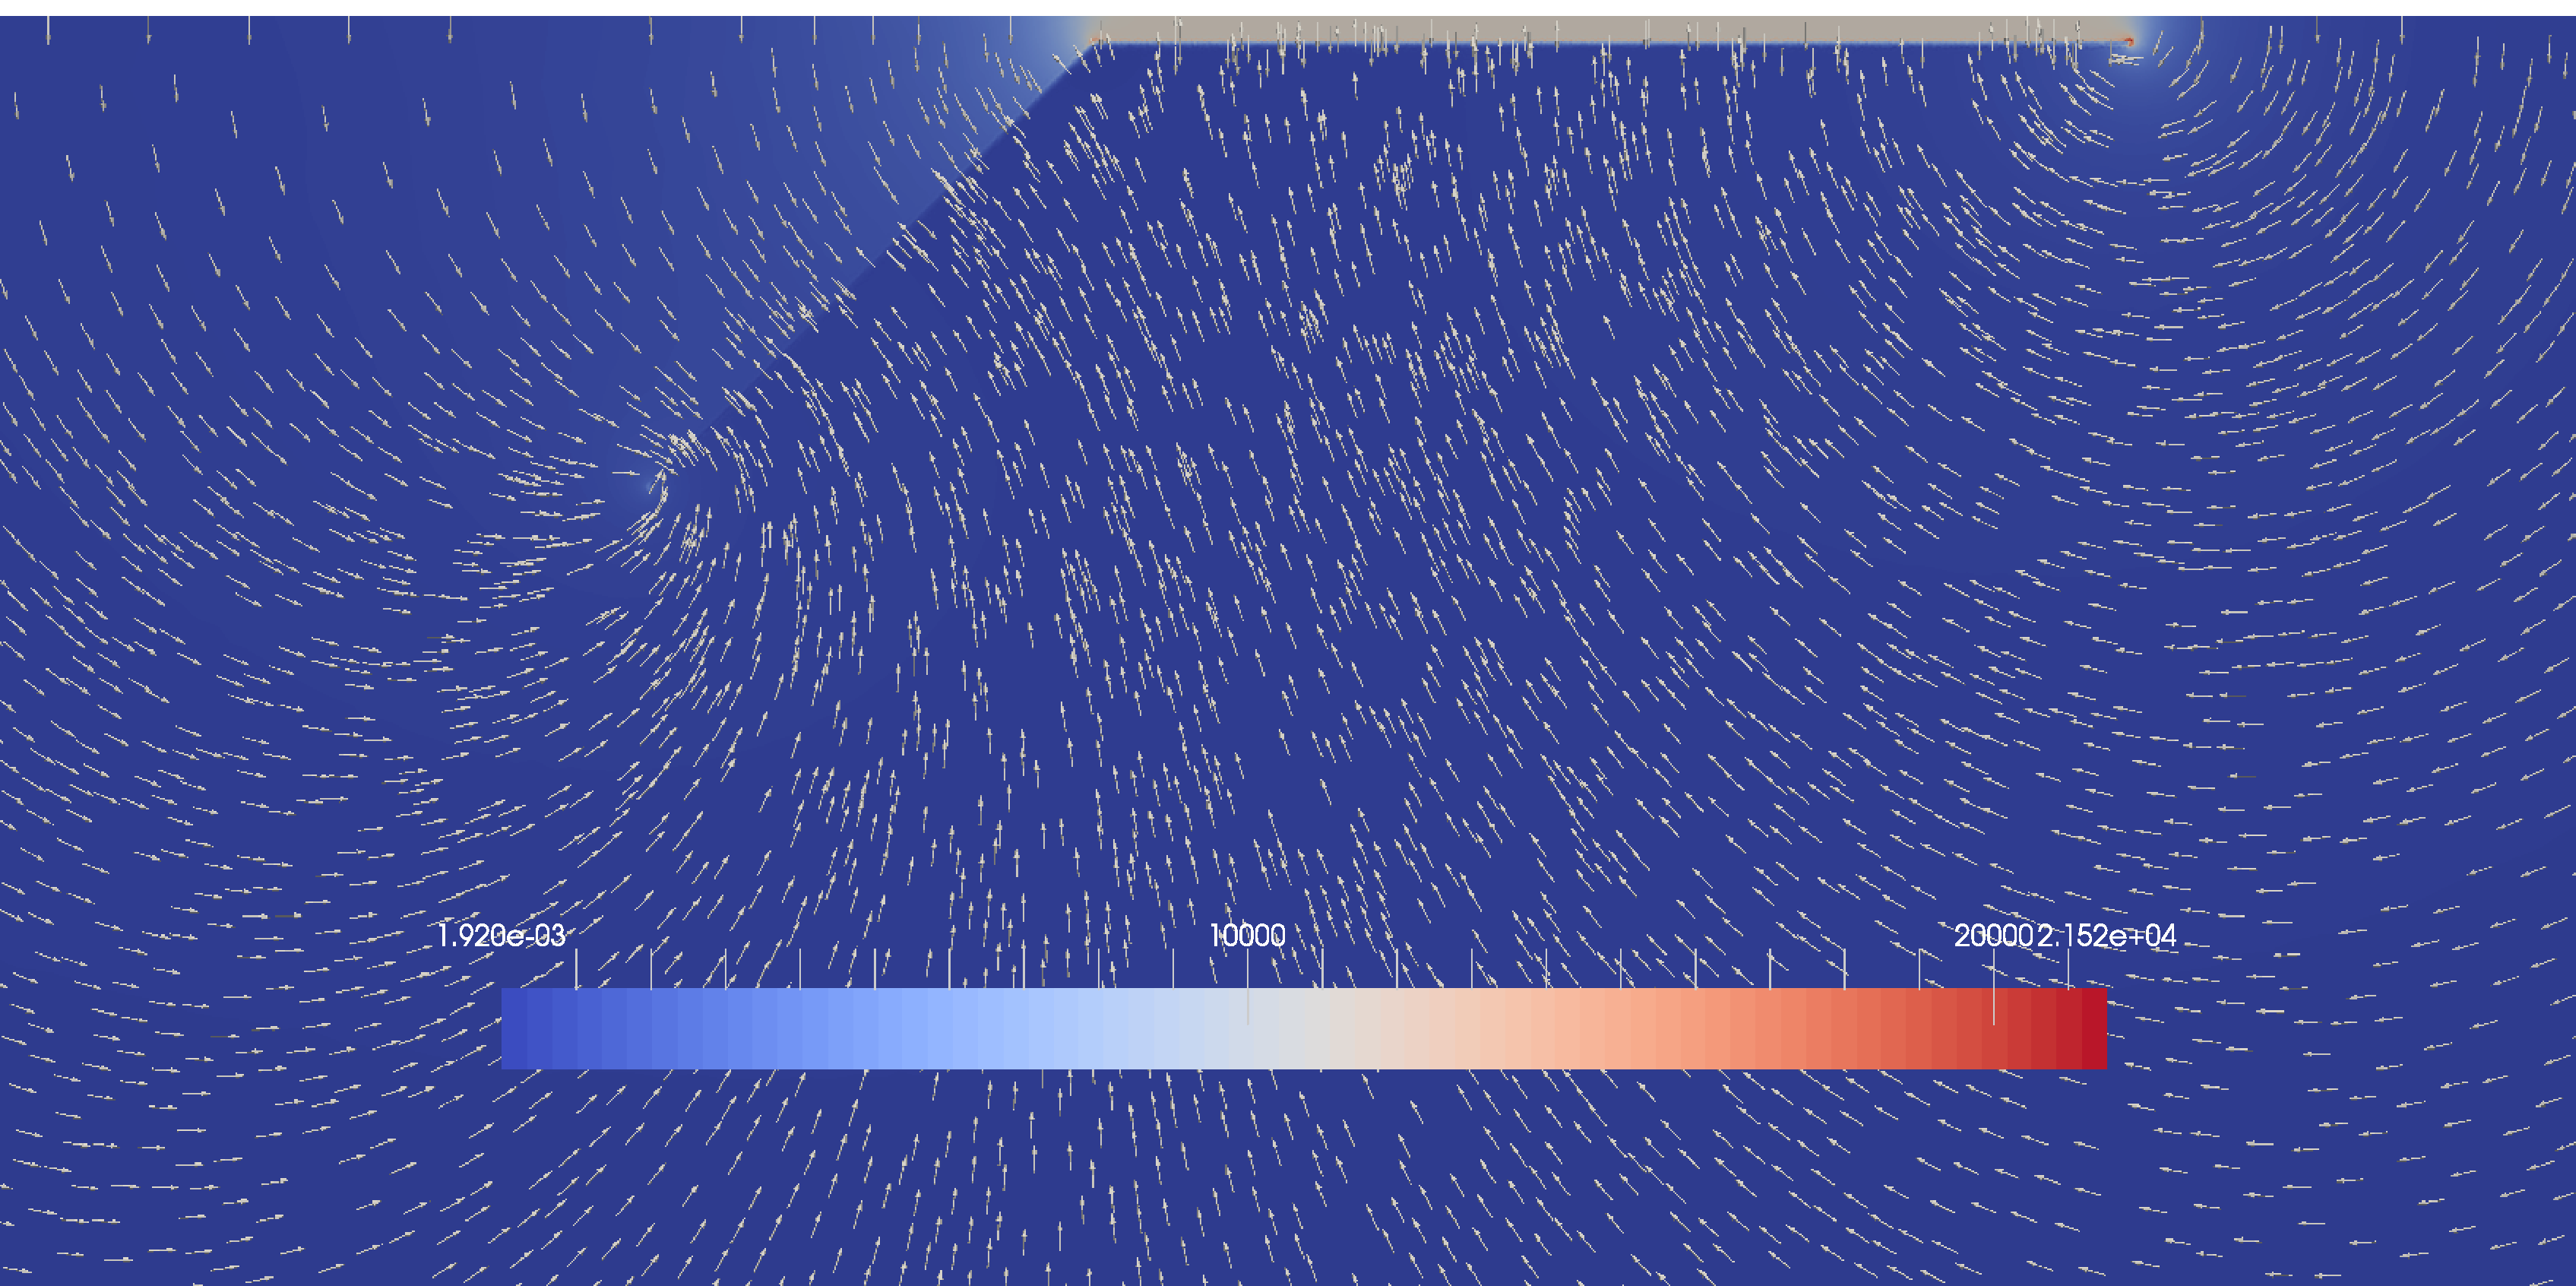
\includegraphics[width = \textwidth]{M4condfield}
\end{figure}
Il metodo descritto presenta alcune limitazioni: infatti si trascura intrinsecamente qualsiasi contributo tangenziale (fuori dal piano delle sezioni). In questa analisi l'effetto è trascurabile poiché anche in presenza di un angolo relativo la soluzione resta prevalentemente nel piano delle sezioni. 

Si aggiunge che questa tecnica di calcolo si presta anche alla valutazione della variazione di capacità rispetto ad effetti di ordine superiore (ad esempio effetti di deformazione di una delle due armature) che in questa sede non sono stati analizzati.
In Figura \ref{fig:M4condsol} è mostrato l'andamento della capacità totale ottenuta per configurazioni considerate. La possibilità di effettuare una analisi bidimensionale ha permesso la ripetizione della simulazione per decine di configurazioni.


\begin{figure}[htb]
\subfloat[][]{
 \begin{tikzpicture}
    \begin{axis}[
    		     width = .8\textwidth,
    		     height = .2\textheight,
                 ylabel = {Capacità $\left(\text{pF}\right)$}, 
                 xlabel = {Distanza verticale $z$ ($\mu$m)}]
    \addplot[black,  mark = triangle*]
    file {./Immagini/ActSens/m4condz.dat};
    \end{axis}
    \end{tikzpicture}
    }\\
\subfloat[][]{
 \begin{tikzpicture}
    \begin{axis}[
    		     width = .8\textwidth,
    		     height = .2\textheight,
    		     ymin = 31.884,
                 ymax = 31.887,
                 ylabel = {Capacità $\left(\text{pF}\right)$}, 
                 xlabel = {Angolo $\alpha$ (°)}]
        \addplot[black, mark = triangle*]
    file {./Immagini/ActSens/m4conda.dat};
    \end{axis}
    \end{tikzpicture}
    }
\caption{Capacità del condensatore: andamento rispetto a scostamenti verticali (a) e rotazioni (b)}
\label{fig:M4condsol}
\end{figure}

L'interpolazione dei risultati ha portato alle seguenti espressioni interpolanti, utilizzabili per la simulazione della lettura nelle analisi successive:
\begin{equation}
\label{eq:6m4cap2d4}
\left\{
\begin{array}{l}
C_0 = 0.0319 \\
C(z) = \left(-298.8 z^2+369.6 z+0.5\right)^{-1}\\
C(\alpha) = 0.09\cdot\alpha^2+0.0319,
\end{array}
\right.
\end{equation}
dove la capacità è espressa in nF, la distanza in mm, l'angolo in radianti. 
% !TEX encoding = UTF-8 Unicode
% !TEX TS-program = pdflatex
% !TEX root = ../Tesi.tex



%************************************************
\myChapter{Specchio e sistema di controllo}
%************************************************
\label{chap:mirror}
Al fine di poter valutare il comportamento del gruppo di controllo analizzato nel Capitolo \ref{chap:ActSens} è stato sviluppato un codice di simulazione strutturale di uno specchio attivo. La scelta è ricaduta su un modello ampiamente utilizzato per prove sperimentali, chiamato \textit{P45} \citep{manettiphd}, integrato con il sistema di controllo digitale soggetto a disturbi opportunamente modellati. L'effetto dell'inserimento del comportamento degli attuatori e dei sensori verrà poi valutato sulle caratteristiche della risposta ad un caratteristico segnale temporale nel Capitolo \ref{chap:simulations}.

\section{Piastra di Mindlin}
Il codice strutturale ad elementi finiti è basato sul modello di piastra di Mindlin. Anche in questo caso sono state sfruttate le librerie di FEniCS per l'assemblaggio delle matrici di rigidezza.
Ai fini della caratterizzazione dello specchio è stato trascurato il movimento \textit{in plane} dello specchio, per il quale la stabilità non è garantita dal sistema di controllo bensì dal sostegno centrale. Nell'ipotesi di un disaccoppiamento completo fra il movimento trasversale e longitudinale, i gradi di libertà considerati identificano tre campi scalari:
\begin{equation}
\label{eq:7plv1}
\T{u} = \left\{
\begin{array}{c}
w\\ \theta_x\\ \theta_y\end{array}\right\},
\end{equation}
dove $w$ è lo spostamento perpendicolare al piano, $\theta_x$ e $\theta_y$ sono, rispettivamente, le rotazioni della sezione attorno agli assi $x$ e $y$ del sistema di riferimento. 

Il lavoro virtuale delle forze elastiche per i gradi di libertà considerati, assumendo stato piano di sforzo e materiale isotropo, può essere scritto come segue:
\begin{align}
\label{eq:7plv2}
&\delta \TTTT{L}_d =\nonumber\\&=
\int_V\delta\left\{
\begin{array}{c}
z \de_x\theta_y\\ 
-z \de_y\theta_x\\ 
z \left(\de_x\theta_x- \de_y\theta_y\right)\\
\theta_y+\de_x w\\
-\theta_x+\de_y w
\end{array}\right\}\cdot
\left\{
\begin{array}{c}
\frac{Ez}{1-\nu^2}\left(\de_x\theta_y- \nu\de_y\theta_x\right)\\
\frac{Ez}{1-\nu^2}\left(\nu\de_x\theta_y- \de_y\theta_x\right)\\
-z G \left(\de_x\theta_x- \de_y\theta_y\right)\\
G\left(\theta_y+\de_x w\right)\\
G\left(-\theta_x+\de_y w\right)
\end{array}\right\}dv,
\end{align}
dove:
\begin{equation}
\label{eq:7plv3}
\left\{\begin{array}{l}
E\text{ è il modulo di Young}\\
\nu\text{ è il coefficiente di Poisson}\\
G = \frac{E}{2\left(1+\nu\right)}\text{ è il modulo di rigidezza a taglio.}
\end{array}\right.\nonumber
\end{equation}

Riorganizzando l'equazione e isolando i contributi flessionali e di taglio si ottiene:
\begin{equation}
\label{eq:7plv4}
\delta \TTTT{L}_d = \int_V\left(\delta\T{\varepsilon_{fl}}\cdot\TT{\hat{E}_{fl}}\T{\varepsilon_{fl}} +G\delta\T{\varepsilon_{t}}\cdot\T{\varepsilon_{t}}\right)dv,
\end{equation}
con
\begin{align}
\label{eq:7plv5}
&\T{\varepsilon_{fl}} = \left\{
\begin{array}{c}
\de_x\theta_y\\ 
\de_y\theta_x\\ 
\de_x\theta_x- \de_y\theta_y
\end{array}\right\},\\
\label{eq:7plv5bis}
&\TT{\hat{E}_{fl}} = \frac{Ez^2}{1-\nu^2}\left[\begin{array}{ccc}
1 & -\nu & 0\\-\nu & 1 & 0\\0&0& \frac{G\left(1-\nu^2\right)}{E}\end{array}\right],\\
\label{eq:7plv5tris}
&\T{\varepsilon_{t}} = \left\{
\begin{array}{c}
\theta_y+\de_x w\\ 
-\theta_x+\de_y w
\end{array}\right\}.
\end{align}

Dividendo l'integrale di volume, si ha:
\begin{align}
\label{eq:7plv6}
\delta \TTTT{L}_d &= \int_A\int_{-t/2}^{t/2}\left(\delta\T{\varepsilon_{fl}}\cdot\TT{\hat{E}_{fl}}\T{\varepsilon_{fl}} +G\delta\T{\varepsilon_{t}}\cdot\T{\varepsilon_{t}}\right)dzdA\\
\label{eq:7plv6bis} &= \int_A\left(\delta\T{\varepsilon_{fl}}\cdot\TT{E_{fl}}\T{\varepsilon_{fl}} +Gt\delta\T{\varepsilon_{t}}\cdot\T{\varepsilon_{t}}\right)dA,
\end{align}
dove 
\begin{equation}
\label{eq:7plv7}
\TT{\hat{E}_{fl}} = \frac{Et^3}{12\left(1-\nu^2\right)}\left[\begin{array}{ccc}
1 & -\nu & 0\\-\nu & 1 & 0\\0&0& \frac{G\left(1-\nu^2\right)}{E}\end{array}\right].
\end{equation}

Il lavoro delle forze d'inerzia può essere espresso come\footnote{Per semplificare la notazione, in ambito strutturale si preferisce indicare la derivata temporale di una quantità $x$ con $\dot{x}$ anziché $\de_t x$.}:
\begin{align}
\label{eq:7plv8}
\delta\TTTT{L}_i &=-\int_A \int_{-t/2}^{t/2} \delta\T{u}
\cdot
\left[
\begin{array}{ccc}
\rho & \rho z & \rho z \\
\rho z & \rho z^2 & 0 \\
\rho z & 0 & \rho z^2
\end{array}
\right]\ddot{\T{u}}~dzdA\\
\label{eq:7plv8.1}
& = 
-\int_A \delta\T{u}
\cdot
\left[
\begin{array}{ccc}
\rho t & 0 & 0 \\
0 & \rho\frac{t^3}{12} & 0 \\
0 & 0 & \rho \frac{t^3}{12}
\end{array}
\right]\ddot{\T{u}}~dA\\
\label{eq:7plv8.2}
 &=- \int_A \delta\T{u} \TT{M_l}\ddot{\T{u}}~dA.
\end{align}
Il contributo di masse e inerzie concentrate può essere aggiunto:
\begin{align}
\label{eq:7plv8bis}
\delta\TTTT{L}_i &=-\delta\T{u}\left(x_P,y_P\right)
\cdot \TT{M_P}~\ddot{\T{u}}\left(x_P,y_P\right)\\
\label{eq:7plv8bis2}
&= \lfloor\T{u}\cdot \TT{M_P}~\ddot{\T{u}} \rfloor_{\left(x_P,y_P\right)}.
\end{align}
Infine, il lavoro delle forze e coppie esterne può essere scritto, separando contributi superficiali e concentrati, come:
\begin{align}
\label{eq:7plv9}
\delta\TTTT{L}_e &=\int_A \delta\T{u}
\cdot \left\{\begin{array}{c}f_z\\c_x\\c_y\end{array}\right\}dA 
+ \delta\T{u}\left(x_P,y_P\right)
\cdot \left\{\begin{array}{c}F_z\left(x_P,y_P\right)\\C_x\left(x_P,y_P\right)\\C_y\left(x_P,y_P\right)\end{array}\right\}\\
& = 
\int_A \delta\T{u}
\cdot
\T{f}~dA+\lfloor\T{u}\cdot \T{F} \rfloor_{\left(x_P,y_P\right)}.
\end{align}
La dinamica della piastra può essere allora espressa tramite l'equazione in forma variazionale:
\begin{equation}
\label{eq:7plv10}
\delta \TTTT{L}_d = \delta \TTTT{L}_i + \delta \TTTT{L}_e
\end{equation}


Per lo smorzamento strutturale viene utilizzato il modello proporzionale:
\begin{equation}
\label{eq:7plv11}
\TT{C} = \alpha \TT{M}+\beta\TT{K}.
\end{equation}

I valori $\alpha$ e $\beta$ sono stati ottenuti imponendo due valori di fattore di smorzamento desiderati $\xi_{1,2}$ per due pulsazioni caratteristiche $\omega_{1,2}$ e risolvendo il sistema lineare:
\begin{equation}
\label{eq:7plv12}
\left\{
\begin{array}{c}
2\xi_1\omega_1 = \alpha+\beta\omega_1^2\\
2\xi_2\omega_2 = \alpha+\beta\omega_2^2\\
\end{array}\right.
\end{equation}

I valori sono stati scelti per rappresentare i contributi di dissipazione strutturale e fluidodinamica.\\

Per non incorrere nel fenomeno dello \textit{shear locking} (e la conseguente erronea distribuzione dei contributi energetici di deformazione fra flessione e taglio) è sufficiente porre attenzione agli ordini degli elementi per gli spazi funzionali considerati: in particolare, gli elementi del campo $w$ devono essere superiori agli altri di almeno un ordine. In questo lavoro si è fatto uso di elementi lagrangiani di ordine 3 per lo spostamento $w$ e di ordine 2 per le rotazioni $\theta_x$ e $\theta_y$.

Assemblando le matrici, il sistema assume la consueta forma:

\begin{equation}
\label{eq:7plv13}
\TT{M}\ddot{\T{x}}+\TT{C}\ddot{\T{x}}+\TT{K}\T{x} = \T{q}.
\end{equation}
\subsection{Test-case: pannello rettangolare}

In questa sezione verrà validato il modello strutturale mediante confronti con il solutore commerciale MSC Nastran. I confronti riguardano analisi statiche con carichi distribuiti o concentrati ed estrazioni modali. 

Il confronto è stato effettuato per un pannello rettangolare. I dati geometrici e strutturali del pannello sono elencati in Tabella \ref{tab:7rettangolo1}.\\

\begin{table}[htb]
\caption{Pannello rettangolare: dati del modello}
\label{tab:7rettangolo1}
\centering
\begin{tabular}{lcc}
\toprule
Lato 1 & $l_x$ & 10 m \\
Lato 2 & $l_y$ & 5 m \\
Modulo di Young & $E$ & 72 GPa\\
Coeff. di Poisson & $\nu$ & 0.3\\
Forza verticale nel nodo $A$& $F_A$ & 3 N\\
Forza verticale nel nodo $B$& $F_B$ & -2 N\\
\bottomrule
\end{tabular}
\end{table}

Come prima analisi, è stato imposto un vincolo d'incastro su uno dei lati corti e applicati due carichi concentrati di entità diversa agli estremi del lato opposto a quello vincolato. Questa condizione è utile per la verifica dell'assenza di \textit{shear-locking}.

Lo spostamento ottenuto con i due codici è riportato in Tabella \ref{tab:7rettangolo2}. Come si può vedere, le differenze sono estremamente basse; la soluzione è sostanzialmente coincidente.

\begin{figure}[h]
\centering
\caption{Pannello rettangolare soggetto a carichi concentrati: confronto sulla deformata }
\label{fig:7rettangolowconf}
\subfloat[][FEniCS]{
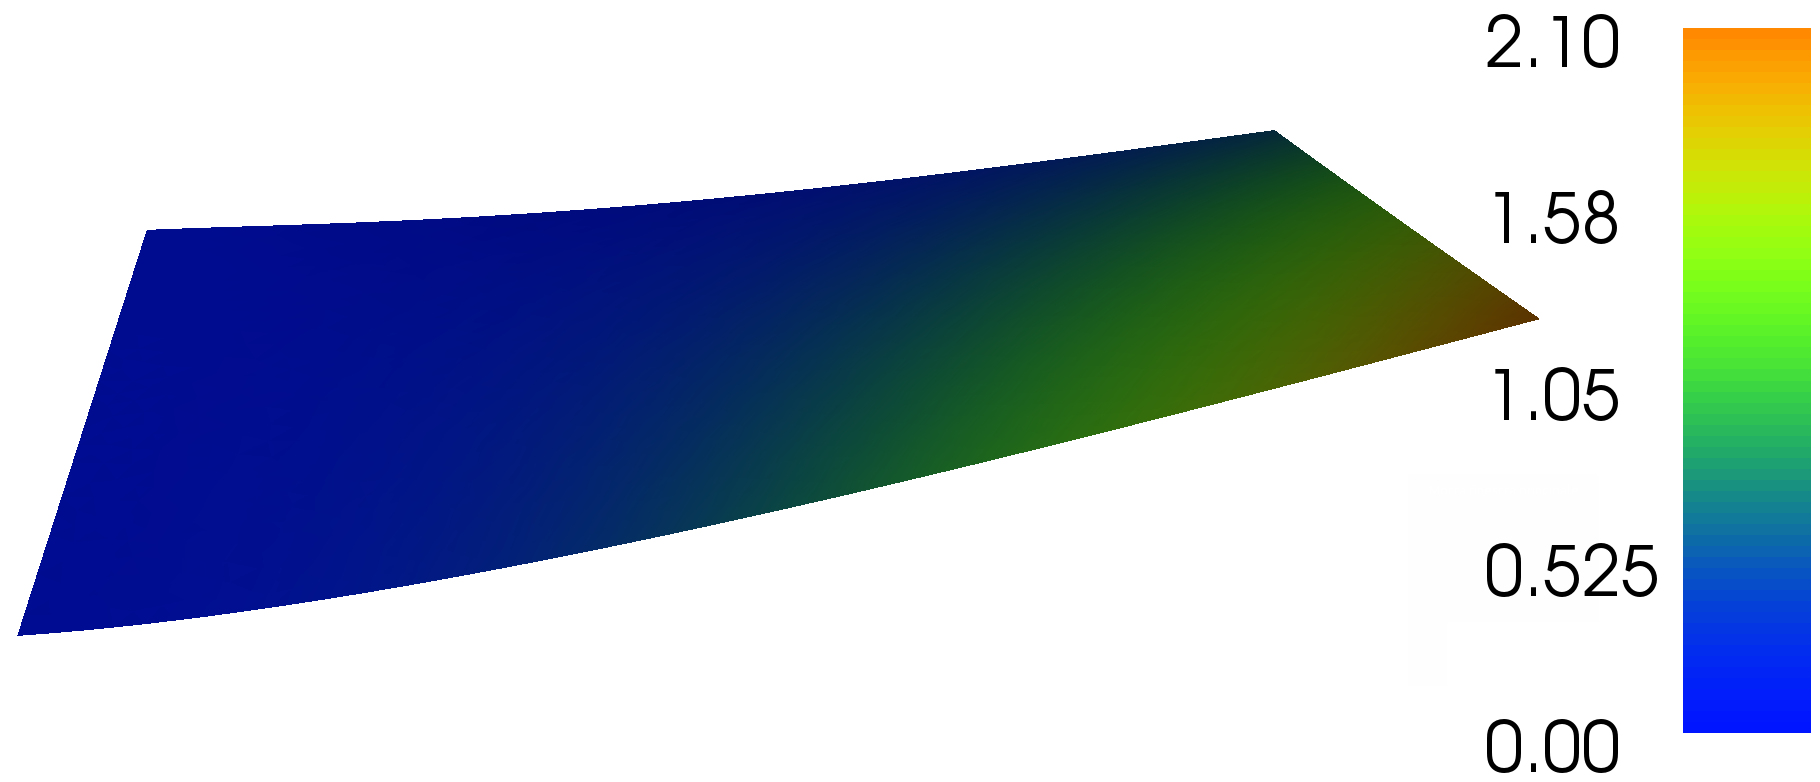
\includegraphics[width = .48\textwidth]{rettangolow}}
\subfloat[][Nastran]{
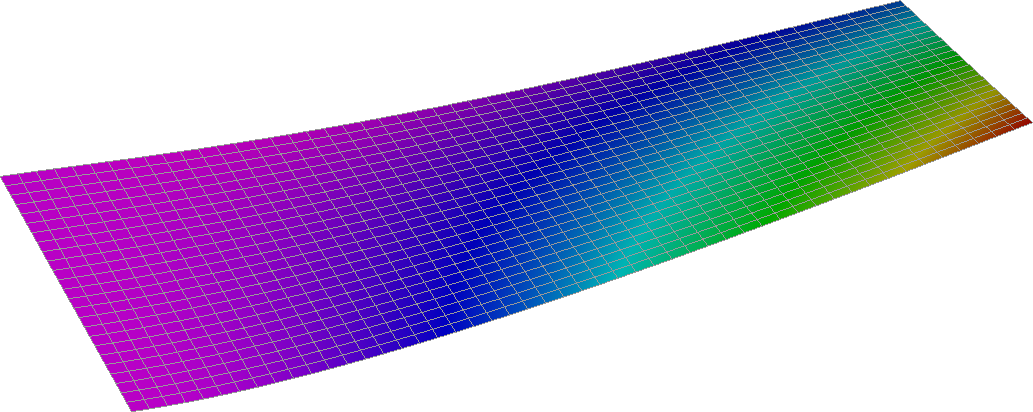
\includegraphics[width = .38\textwidth]{rettangolownastran}}
\end{figure}


\begin{table}[h]
\caption{Pannello rettangolare soggetto a carichi concentrati: confronto fra gli spostamenti massimi}
\label{tab:7rettangolo2}
\centering
\begin{tabular}{lc}
\toprule
~&Spostamento del nodo $A$\\
FEniCS & 2.0799 m\\
Nastran & 2.0787 m\\
\bottomrule
\end{tabular}
\end{table}


In seguito, per verificare la corretta integrazione delle forze superficiali, sul pannello sono stati applicati un vincolo di appoggio su tutti i lati e una pressione costante pari a 0.05 Pa. 

Lo scostamento massimo è mostrato in Tabella \ref{tab:7rettangolo3}. Anche in questo caso le soluzioni sono sostanzialmente coincidenti.

\begin{figure}[h]
\centering
\caption{Pannello rettangolare soggetto a carichi distribuiti: confronto sulla deformata}
\label{fig:7rettangolowconf2}
\subfloat[][FEniCS]{
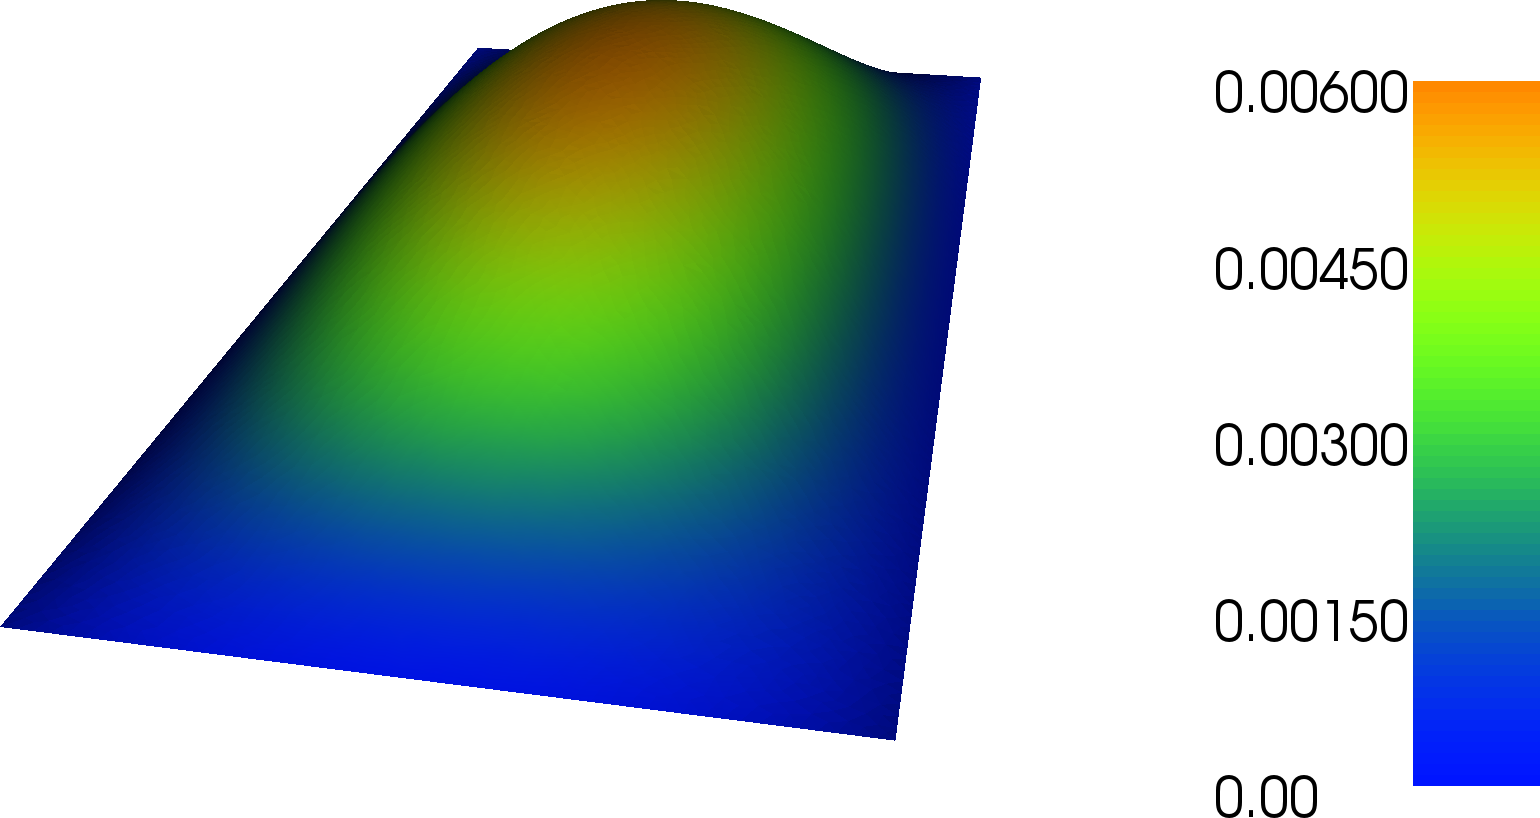
\includegraphics[width = .48\textwidth ]{rettangolowpressure}}
\subfloat[][Nastran]{
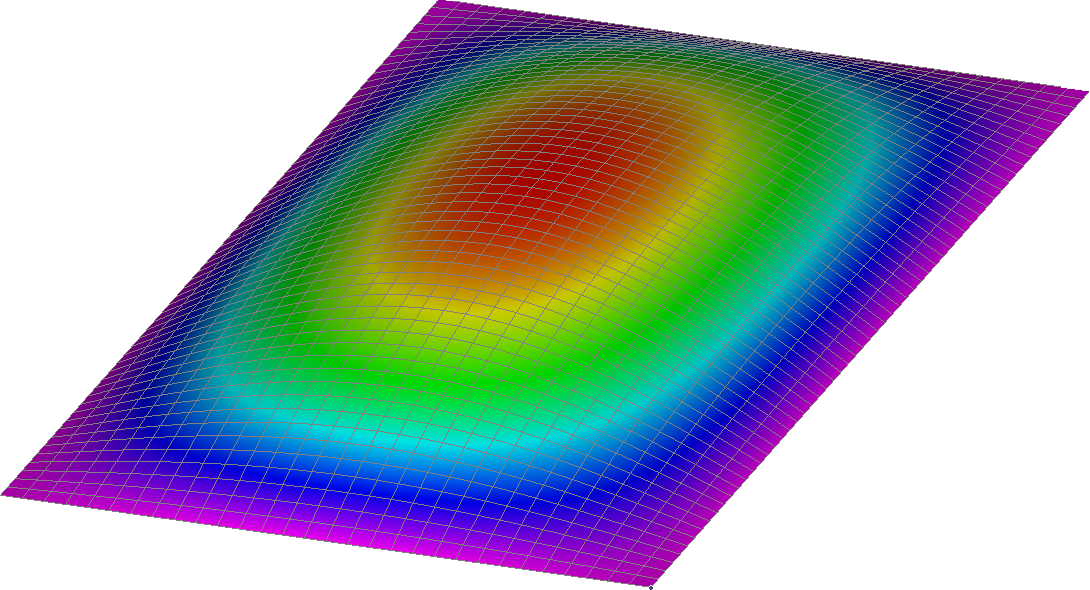
\includegraphics[width = .38\textwidth]{rettangolowpressurenastran}}
\end{figure}


\begin{table}[htb]
\caption{Pannello rettangolare soggetto a carichi distribuiti: confronto fra gli scostamenti massimi}
\label{tab:7rettangolo3}
\centering
\begin{tabular}{lc}
\toprule
~&Scostamento del nodo centrale (massimo)\\
FEniCS & 5.88 mm\\
Nastran & 5.89 mm\\
\bottomrule
\end{tabular}
\end{table}


Infine, in Tabella \ref{tab:7rettangolo4}, si riportano le frequenze ottenute per i primi 20 autovalori in una analisi modale del pannello libero (non smorzato). 

\begin{table}[h]
\caption{Pannello rettangolare: confronto fra le frequenze dei primi 20 modi di vibrare}
\label{tab:7rettangolo4}
\centering
\begin{tabular}{lcclcc}
\toprule
& FEniCS & Nastran &  & FEniCS & Nastran\\
\midrule
1° &  0.00000    Hz & 0.00000   Hz   &   11° &  0.59397     Hz &  0.59384   Hz \\
2° &  0.00000    Hz & 0.00000   Hz   &   12° &  0.71837     Hz &  0.71796   Hz \\
3° &  0.00000    Hz & 0.00000   Hz   &   13° &  0.79599     Hz &  0.79559   Hz \\
4° &  0.10688    Hz & 0.10687   Hz   &   14° &  0.96473     Hz &  0.96420   Hz \\
5° &  0.13084    Hz & 0.13080   Hz   &   15° &  1.01235     Hz &  1.01192   Hz \\
6° &  0.28880    Hz & 0.28870   Hz   &   16° &  1.16824     Hz &  1.16753   Hz \\
7° &  0.29720    Hz & 0.29715   Hz   &   17° &  1.22971     Hz &  1.22906   Hz \\
8° &  0.44063    Hz & 0.44049   Hz   &   18° &  1.30786     Hz &  1.30711   Hz \\
9° &  0.50297    Hz & 0.50276   Hz   &   19° &  1.32918     Hz &  1.32802   Hz \\
10° & 0.51933    Hz & 0.51911   Hz   &   20° &  1.47560     Hz &  1.47435   Hz \\
\bottomrule
\end{tabular}
\end{table}
\clearpage
\section{Schema di controllo}
I sistemi di controllo per gli specchi attualmente in uso devono far fronte a diverse problematiche fra cui l'alta densità modale e il basso smorzamento dei modi ad alta frequenza. Inoltre l'acquisizione, l'elaborazione dei segnali e l'applicazione degli ingressi di controllo richiedono un tempo troppo lungo per un'architettura a ciclo chiuso centralizzata. Per questo la struttura è a più livelli: il segnale di posizione di riferimento elaborato sulla base della misura della distorsione del fronte d'onda viene inviato a tutti gli attuatori mediante un controllo in \textit{feed-forward} centralizzato a frequenza definita sulla base dei tempi caratteristici delle distorsioni (per specchi terrestri, dove la fonte di disturbo più rapida è la turbolenza atmosferica, la frequenza di aggiornamento è variabile tra 1 e 2 kHz). Un ciclo di retroazione decentralizzato a frequenza più alta (attualmente nell'ordine del centinaio di kHz) assicura l'inseguimento del segnale con scostamenti
massimi di 10--20 nm.


Questa architettura permette di sfruttare i vantaggi del controllo
decentralizzato in ciclo chiuso, in particolare l'elevata velocità di elaborazione e la
robustezza rispetto a disturbi ed errori di modellazione, per stabilizzare la forma dello specchio nell'intorno della posizione desiderata \citep{manetti_high_2010}.

\begin{figure}[htb]
\centering
\caption{Raccordo per il segnale in \textit{feed-forward}}
\label{fig:71menocos}
\begin{tikzpicture}
\begin{axis}[width = .8\textwidth,
             height = .2\textheight,             
             ylabel = $f_{sh}$,
			 xlabel = $t$,
			 ticks = none, 
			 ymax = 1.2,
			 axis x line = middle, 
			 axis y line = middle, 
			 enlargelimits,
			 semithick]
\addplot[thick, smooth, samples = 200,domain = 0:180]
{0.5*(1-cos(x))};
\addplot[thick, smooth, samples = 100,domain = 180:500]
{1};
\end{axis}
\end{tikzpicture}
\begin{tikzpicture}
\begin{axis}[width = .8\textwidth,
             height = .2\textheight,  
             ylabel = $\dot{f}_{sh}$,
			 xlabel = $t$,
			 ticks = none, 
			 ymax = 1.2,
			 axis x line = middle, 
			 axis y line = middle, 
			 enlargelimits,
			 semithick]
\addplot[thick, smooth, samples = 200,domain = 0:180]
{sin(x)};
\addplot[thick, smooth, samples = 200,domain = 180:500]
{0};
\end{axis}
\end{tikzpicture}
\begin{tikzpicture}
\begin{axis}[width = .8\textwidth,
             height = .2\textheight,  
             ylabel = $\dot{f}_{sh}$,
			 xlabel = $t$,
			 ticks = none, 
			 ymax = 1.2,
			 axis x line = middle, 
			 axis y line = middle, 
			 enlargelimits,
			 semithick]
\addplot[thick, smooth, samples = 200,domain = 0:180]
{cos(x)};
\addplot[thick, smooth, samples = 200,domain = 180:500]
{0};
\draw {(180,-1)--(180,0)};
\end{axis}
\end{tikzpicture}
\end{figure}

Il segnale di riferimento elaborato è inviato con frequenza $f_{ol}$ e viene mantenuto costante per la durata di un ciclo ($T_{ol} = 1/f_{ol}$). Il segnale complessivo di riferimento per ogni attuatore risulta composto da tratti costanti, che vengono opportunamente raccordati utilizzando funzioni polinomiali o trigonometriche (Figura \ref{fig:71menocos}). Definendo $\T{d_k^r}$ il vettore contenente le posizioni di riferimento al passo corrente per i punti di controllo e $\T{d_{k+1}^r}$ il vettore delle posizioni al passo successivo, la storia temporale da inseguire è:


\begin{align}
\label{eq:7ff1}
\T{r}(t) &= \T{d_k^r}+\left(\T{d_{k+1}^r} -\T{d_k^r}\right)f_{sh}(t)\\
\label{eq:7ff1.0}
\dot{\T{r}}(t) &= \left(\T{d_{k+1}^r} -\T{d_k^r}\right)\dot{f}_{sh}(t)\\
\label{eq:7ff1.1}
\ddot{\T{r}}(t) &= \left(\T{d_{k+1}^r} -\T{d_k^r}\right)\ddot{f}_{sh}(t),
\end{align}
dove $f_sh$ è la funzione di raccordo (\textit{shaping}) normalizzata, tale per cui:
\begin{equation}
\label{eq:7ff2}
\left\{\begin{array}{c}
f_{sh}(0) = 0\\
f_{sh}(\hat{T}) = 1\\
\dot{f}_{sh}(0) = 0\\
\dot{f}_{sh}(\hat{T}) = 0
\end{array}\right.
\end{equation}
e $\hat{T}$ è un tempo caratteristico per il raccordo; per le simulazioni successive è stato utilizzato:
\begin{equation}
\label{eq:7ff3}
\hat{T} = \frac{T_{ol}}{4}.
\end{equation}

Il vettore delle forze in anello aperto è elaborato approssimando la dinamica strutturale sulla base di matrici di rigidezza, massa e smorzamento identificate sperimentalmente $\TT{K^*}$, $\TT{M^*}$, $\TT{C^*}$. Tali matrici sono  simili alle matrici condensate rispetto ai punti di controllo, e differiscono soltanto per l'effetto non lineare della non co-locazione di sensori e attuatori.
\begin{align}
\label{eq:7ff4}
\T{F_{ol}}(t) =& \TT{M^*}\ddot{\T{r}}(t)+\TT{C^*}\dot{\T{r}}(t)+\TT{K^*}\T{r}(t)\nonumber\\
=& \TT{M^*}\left(\T{d_{k+1}^r} -\T{d_k^r}\right)\ddot{f}_{sh}(t)+\nonumber\\
&+\TT{C^*}\left(\T{d_{k+1}^r} -\T{d_k^r}\right)\dot{f}_{sh}(t)+\nonumber\\
&+\TT{K^*}\left[\T{d_k^r}+\left(\T{d_{k+1}^r} -\T{d_k^r}\right)f_{sh}(t)\right].
\end{align}

 
Al contributo del controllore in ciclo aperto viene aggiunto il controllo decentralizzato basato su architettura PD. Identificando con $\tilde{\T{w}}$ il vettore degli spostamenti trasversali $w$ misurati dai sensori, le forze in anello chiuso possono essere scritte come:
\begin{align}
\label{eq:7fb1}
\T{F_{cl}}(t) = \TT{G_p}\left[\T{r}(t)-\tilde{\T{w}}(t)\right]+ \TT{G_d}\left[\dot{\T{r}}(t)-\dot{\tilde{\T{w}}}(t)\right].
\end{align}

Le matrici dei guadagni hanno struttura completamente diagonale per l'architettura de-centralizzata. L'implementazione digitale a tempo discreto del controllo impone l'utilizzo delle misure acquisite nel passo di campionamento precedente. Questo comporta l'introduzione di un ritardo costante nell'applicazione del controllo proporzionale. Il vettore $\dot{\tilde{\T{w}}}$ è ricostruito numericamente con schemi alle differenze finite applicate ai valori di posizione acquisiti nei passi precedenti.

Negli specchi attuali è comune l'introduzione di un contributo integrale, che può essere ottenuto sia attraverso il controllo in ciclo chiuso (aggiungendo il contributo allo schema \textit{PD}), sia attraverso l'utilizzo di un contributo ricorsivo in anello aperto detto controllo \textit{ossimorinico} o \textit{ibrido} \citep{manetti_self-tuning_2014}. In questo lavoro è stato implementato il secondo metodo: considerando il passo di controllo $k$, nella fase in cui la posizione viene mantenuta statica viene registrata una media della misura dello spostamento del punto di controllo. Questa media viene utilizzata per la costruzione del contributo di forza in feed-forward al passo $k+1$: la forza inviata dal controllore centralizzato non è più propriamente in anello aperto poiché contiene delle informazioni sullo stato del sistema. Il contributo ibrido si ottiene sostituendo il valore mediato $\T{\bar{w}}_k$ a $d^r_k$ e sostituendo il termine statico $\TT{K^*}\bar{\T{w}}_k$ con la forza media $\bar{\T{F}}_k$ (le medie sono calcolate nella fase finale del passo precedente, in cui la posizione è mantenuta costante):

\begin{align}
\label{eq:7foxy}
\T{F_{oxy}}(t) =& \TT{M^*}\left(\T{d_{k+1}^r} -\T{\bar{w}}_k\right)\ddot{f}_{sh}(t)+\nonumber\\
&+\TT{C^*}\left(\T{d_{k+1}^r} -\T{\bar{w}}_k\right)\dot{f}_{sh}(t)+\nonumber\\
&+\TT{K^*}\left(\T{d_{k+1}^r} -\T{\bar{w}}_k\right)f_{sh}(t)+\bar{\T{F}}_k.
\end{align}


\section{Integratore implicito}

Per le simulazioni di risposta è stato implementato un metodo di integrazione implicito a due passi a dissipazione numerica modulabile \citep{masarati_efficient_2014}. Il metodo è così strutturato:
\begin{equation}
\label{eq:7metodo1}
x_{k+1} = a_0x_k+a_{-1}x_{k-1}+b_1\dot{x}_{k+1}+b_0\dot{x}_k+b_{-1}\dot{x}_{k-1},
\end{equation}
dove
\begin{align}
\label{eq:7metodo2.0}
&\alpha = \Delta t_p /\Delta t_c,\\
\label{eq:7metodo2.1}
&\beta = \alpha\frac{(2+\alpha)(1-\rho_\infty)^2+2(1+\alpha)(2\rho_\infty-1)}{2(1+\alpha)-(1-\rho_\infty)^2},\\
\label{eq:7metodo2.2}
&\delta = \frac{\alpha^2(1-\rho_\infty)^2}{2(2(1+\alpha)-(1-\rho_\infty)^2)},\\
\label{eq:7metodo2.3}
&a_0 = 1-\beta,\\
\label{eq:7metodo2.4}
&a_{-1} = \beta,\\
\label{eq:7metodo2.5}
&b_1 = \Delta t_c \left(\frac{\delta}{\alpha}+\frac{\alpha}{2}\right),\\
\label{eq:7metodo2.6}
&b_0 = \Delta t_c\left(\frac{\beta}{2}+\frac{\alpha}{2} -(1+\alpha)\frac{\delta}{\alpha}\right),\\
\label{eq:7metodo2.7}
&b_{-1} = \Delta t_c \left(\frac{\beta}{2}+\delta\right).\\
\end{align}

I parametri per la definizione delle costanti del metodo sono $\Delta t_p$ e $\Delta t_p$ (intervalli di avanzamento precedente e corrente) e $\rho_\infty$ (per la regolazione del filtraggio ad alte frequenze). Scegliendo opportunamente $\rho_\infty$ si bilanciano le proprietà di precisione alle basse frequenze e di filtraggio alle alte frequenze. Per la valutazione degli effetti di \textit{spill-over} si è scelto di limitare il filtraggio, utilizzando alle alte frequenze la sola dissipazione strutturale. Per questo sono stati usati valori di $\rho_\infty$ prossimi a 1. Applicando il metodo di integrazione al sistema strutturale \eqref{eq:7plv13} si ottiene:
\begin{equation}
\label{eq:7metodo3}
\left(\TT{M}+b_1\TT{C}+b_1^2\TT{K}\right)\ddot{\T{x}}_{k+1} = \T{q}_{k+1}-\TT{C}\T{v}_{k,k-1}-\TT{K}\T{u}_{k,k-1}\:,
\end{equation}
dove
\begin{align}
\label{eq:7metodo4.0}
\T{u}_{k,k-1} =& a_0\T{x}_k+a_{-1}\T{x}_{k-1}+\left(b_1a_0+b_0\right)\dot{\T{x}}_k+\nonumber\\
&+\left(b_1a_{-1}+b_{-1}\right)\dot{\T{x}}_{k-1}+ b_1b_0\ddot{\T{x}}_k+\nonumber\\
&+b_1b_{-1}\ddot{\T{x}}_{k-1},\\
\label{eq:7metodo4.1}
\T{v}_{k,k-1} =& a_0\dot{\T{x}}_k+a_{-1}\dot{\T{x}}_{k-1}+ b_0\ddot{\T{x}}_k+b_{-1}\ddot{\T{x}}_{k-1}.
\end{align}

\section{P45}

Come anticipato nell'introduzione di questo capitolo, la simulaizione del sistema di controllo è stata effettuata utilizzando i dati dello specchio $P45$, i cui dati geometrici e strutturali sono riportati in Tabella \ref{tab:7p45data}. Lo specchio è realizzato in \textit{Zerodur\sffamily\textregistered}, un materiale vetro-ceramico comune ad altre strutture adattive attualmente in uso. Il materiale è stato scelto per alcune proprietà importanti per le applicazioni ottiche, come il coefficiente di dilatazione termica quasi nullo e la possibilità di essere lucidato ad alti livelli di precisione.
Lo specchio possiede una debole curvatura che ai fini della simulazione del comportamento flessionale della piastra è trascurabile.\\

\begin{table}[hb]
\caption{Geometria e materiale per lo specchio $P45$}
\label{tab:7p45data}
\centering
\begin{tabular}{lc}
\toprule
Raggio interno & 0.12 m\\
Raggio esterno & 0.2834 m\\
Spessore & 1.61 mm\\
\midrule
Materiale & \textit{Zerodur\sffamily\textregistered}\\
\midrule
Modulo di Young & 91 GPa\\
Coefficiente di Poisson &  0.24\\
Densità & 2.53 g/$\text{cm}^3$\\
\bottomrule
\end{tabular}
\end{table}

La struttura è vincolata al centro attraverso una membrana elastica. Tuttavia questo vincolo è più rigido per i gradi di libertà \textit{in-plane} e il suo contributo trasversale può essere trascurato. Omettendo il vincolo centrale, la struttura è a tutti gli effetti labile e tenuta in equilibrio dinamico dalle sole forze di controllo.\\

\begin{figure}[htb]
\centering
\caption{Mappa dei punti di controllo per il $P45$: sensori (in grigio) e attuatori (in nero)}
\label{fig:7p45map}
\resizebox{.6\textwidth}{!}{
\begin{tikzpicture}
\filldraw[fill = black!20!white, draw = black, very thin](-2.35000e-02*100 , 1.03050e-01*100) circle(0.0145*100);
\filldraw[fill = black!20!white, draw = black, very thin](-5.29000e-02*100 , 9.15350e-02*100) circle(0.0145*100);
\filldraw[fill = black!20!white, draw = black, very thin](-9.52000e-02*100 , 4.58599e-02*100) circle(0.0145*100);
\filldraw[fill = black!20!white, draw = black, very thin](-1.04520e-01*100 , 1.57519e-02*100) circle(0.0145*100);
\filldraw[fill = black!20!white, draw = black, very thin](-1.04520e-01*100 ,-1.58000e-02*100) circle(0.0145*100);
\filldraw[fill = black!20!white, draw = black, very thin](-5.29000e-02*100 ,-9.14999e-02*100) circle(0.0145*100);
\filldraw[fill = black!20!white, draw = black, very thin]( 7.89899e-03*100 ,-1.05399e-01*100) circle(0.0145*100);
\filldraw[fill = black!20!white, draw = black, very thin]( 3.86149e-02*100 ,-9.83900e-02*100) circle(0.0145*100);
\filldraw[fill = black!20!white, draw = black, very thin](-7.74999e-02*100 , 7.18919e-02*100) circle(0.0145*100);
\filldraw[fill = black!20!white, draw = black, very thin]( 7.89899e-03*100 , 1.05399e-01*100) circle(0.0145*100);
\filldraw[fill = black!20!white, draw = black, very thin]( 6.59000e-02*100 , 8.26360e-02*100) circle(0.0145*100);
\filldraw[fill = black!20!white, draw = black, very thin]( 8.73300e-02*100 , 5.95409e-02*100) circle(0.0145*100);
\filldraw[fill = black!20!white, draw = black, very thin]( 1.01000e-01*100 , 3.11540e-02*100) circle(0.0145*100);
\filldraw[fill = black!20!white, draw = black, very thin]( 1.01000e-01*100 ,-3.11999e-02*100) circle(0.0145*100);
\filldraw[fill = black!20!white, draw = black, very thin]( 6.59000e-02*100 ,-8.26000e-02*100) circle(0.0145*100);
\filldraw[fill = black!20!white, draw = black, very thin](-7.74999e-02*100 ,-7.19000e-02*100) circle(0.0145*100);
\filldraw[fill = black!20!white, draw = black, very thin]( 6.83399e-02*100 ,-3.04000e-02*100) circle(0.0145*100);
\filldraw[fill = black!20!white, draw = black, very thin](-7.32000e-02*100 , 1.55530e-02*100) circle(0.0145*100);
\filldraw[fill = black!20!white, draw = black, very thin](-4.13000e-02*100 , 1.50160e-02*100) circle(0.0145*100);
\filldraw[fill = black!20!white, draw = black, very thin](-4.13000e-02*100 ,-1.49999e-02*100) circle(0.0145*100);
\filldraw[fill = black!20!white, draw = black, very thin](-6.05199e-02*100 , 4.39710e-02*100) circle(0.0145*100);
\filldraw[fill = black!20!white, draw = black, very thin]( 6.83399e-02*100 , 3.04269e-02*100) circle(0.0145*100);
\filldraw[fill = black!20!white, draw = black, very thin](-7.82000e-03*100 , 7.43970e-02*100) circle(0.0145*100);
\filldraw[fill = black!20!white, draw = black, very thin]( 2.31169e-02*100 , 7.11460e-02*100) circle(0.0145*100);
\filldraw[fill = black!20!white, draw = black, very thin]( 5.00560e-02*100 , 5.55929e-02*100) circle(0.0145*100);
\filldraw[fill = black!20!white, draw = black, very thin](-7.32000e-02*100 ,-1.55999e-02*100) circle(0.0145*100);
\filldraw[fill = black!20!white, draw = black, very thin](-7.82000e-03*100 ,-7.43999e-02*100) circle(0.0145*100);
\filldraw[fill = black!20!white, draw = black, very thin](-3.74000e-02*100 ,-6.47999e-02*100) circle(0.0145*100);
\filldraw[fill = black!20!white, draw = black, very thin]( 4.39039e-02*100 , 0.00000e+00*100) circle(0.0145*100);
\filldraw[fill = black!20!white, draw = black, very thin](-2.19999e-02*100 , 3.80220e-02*100) circle(0.0145*100);
\filldraw[fill = black!20!white, draw = black, very thin]( 7.62399e-03*100 ,-4.32000e-02*100) circle(0.0145*100);
\filldraw[fill = black!20!white, draw = black, very thin]( 7.62399e-03*100 , 4.32369e-02*100) circle(0.0145*100);
\filldraw[fill = black!20!white, draw = black, very thin]( 3.36320e-02*100 , 2.82210e-02*100) circle(0.0145*100);
\filldraw[fill = black!20!white, draw = black, very thin](-2.35000e-02*100 ,-1.03050e-01*100) circle(0.0145*100);
\filldraw[fill = black!20!white, draw = black, very thin]( 2.31169e-02*100 ,-7.11999e-02*100) circle(0.0145*100);
\filldraw[fill = black!20!white, draw = black, very thin](-9.52000e-02*100 ,-4.58599e-02*100) circle(0.0145*100);
\filldraw[fill = black!20!white, draw = black, very thin]( 1.05700e-01*100 , 0.00000e+00*100) circle(0.0145*100);
\filldraw[fill = black!20!white, draw = black, very thin]( 8.73300e-02*100 ,-5.94999e-02*100) circle(0.0145*100);
\filldraw[fill = black!20!white, draw = black, very thin](-6.05199e-02*100 ,-4.39999e-02*100) circle(0.0145*100);
\filldraw[fill = black!20!white, draw = black, very thin]( 5.00560e-02*100 ,-5.55999e-02*100) circle(0.0145*100);
\filldraw[fill = black!20!white, draw = black, very thin]( 7.48069e-02*100 , 0.00000e+00*100) circle(0.0145*100);
\filldraw[fill = black!20!white, draw = black, very thin](-3.74000e-02*100 , 6.47849e-02*100) circle(0.0145*100);
\filldraw[fill = black!20!white, draw = black, very thin]( 3.36320e-02*100 ,-2.81999e-02*100) circle(0.0145*100);
\filldraw[fill = black!20!white, draw = black, very thin](-2.19999e-02*100 ,-3.79999e-02*100) circle(0.0145*100);
\filldraw[fill = black!20!white, draw = black, very thin]( 3.86149e-02*100 , 9.83900e-02*100) circle(0.0145*100);
\filldraw[fill = white, draw = black, very thin](-2.35000e-02*100 , 1.03050e-01*100) circle(0.011*100);
\filldraw[fill = white, draw = black, very thin](-5.29000e-02*100 , 9.15350e-02*100) circle(0.011*100);
\filldraw[fill = white, draw = black, very thin](-9.52000e-02*100 , 4.58599e-02*100) circle(0.011*100);
\filldraw[fill = white, draw = black, very thin](-1.04520e-01*100 , 1.57519e-02*100) circle(0.011*100);
\filldraw[fill = white, draw = black, very thin](-1.04520e-01*100 ,-1.58000e-02*100) circle(0.011*100);
\filldraw[fill = white, draw = black, very thin](-5.29000e-02*100 ,-9.14999e-02*100) circle(0.011*100);
\filldraw[fill = white, draw = black, very thin]( 7.89899e-03*100 ,-1.05399e-01*100) circle(0.011*100);
\filldraw[fill = white, draw = black, very thin]( 3.86149e-02*100 ,-9.83900e-02*100) circle(0.011*100);
\filldraw[fill = white, draw = black, very thin](-7.74999e-02*100 , 7.18919e-02*100) circle(0.011*100);
\filldraw[fill = white, draw = black, very thin]( 7.89899e-03*100 , 1.05399e-01*100) circle(0.011*100);
\filldraw[fill = white, draw = black, very thin]( 6.59000e-02*100 , 8.26360e-02*100) circle(0.011*100);
\filldraw[fill = white, draw = black, very thin]( 8.73300e-02*100 , 5.95409e-02*100) circle(0.011*100);
\filldraw[fill = white, draw = black, very thin]( 1.01000e-01*100 , 3.11540e-02*100) circle(0.011*100);
\filldraw[fill = white, draw = black, very thin]( 1.01000e-01*100 ,-3.11999e-02*100) circle(0.011*100);
\filldraw[fill = white, draw = black, very thin]( 6.59000e-02*100 ,-8.26000e-02*100) circle(0.011*100);
\filldraw[fill = white, draw = black, very thin](-7.74999e-02*100 ,-7.19000e-02*100) circle(0.011*100);
\filldraw[fill = white, draw = black, very thin]( 6.83399e-02*100 ,-3.04000e-02*100) circle(0.011*100);
\filldraw[fill = white, draw = black, very thin](-7.32000e-02*100 , 1.55530e-02*100) circle(0.011*100);
\filldraw[fill = white, draw = black, very thin](-4.13000e-02*100 , 1.50160e-02*100) circle(0.011*100);
\filldraw[fill = white, draw = black, very thin](-4.13000e-02*100 ,-1.49999e-02*100) circle(0.011*100);
\filldraw[fill = white, draw = black, very thin](-6.05199e-02*100 , 4.39710e-02*100) circle(0.011*100);
\filldraw[fill = white, draw = black, very thin]( 6.83399e-02*100 , 3.04269e-02*100) circle(0.011*100);
\filldraw[fill = white, draw = black, very thin](-7.82000e-03*100 , 7.43970e-02*100) circle(0.011*100);
\filldraw[fill = white, draw = black, very thin]( 2.31169e-02*100 , 7.11460e-02*100) circle(0.011*100);
\filldraw[fill = white, draw = black, very thin]( 5.00560e-02*100 , 5.55929e-02*100) circle(0.011*100);
\filldraw[fill = white, draw = black, very thin](-7.32000e-02*100 ,-1.55999e-02*100) circle(0.011*100);
\filldraw[fill = white, draw = black, very thin](-7.82000e-03*100 ,-7.43999e-02*100) circle(0.011*100);
\filldraw[fill = white, draw = black, very thin](-3.74000e-02*100 ,-6.47999e-02*100) circle(0.011*100);
\filldraw[fill = white, draw = black, very thin]( 4.39039e-02*100 , 0.00000e+00*100) circle(0.011*100);
\filldraw[fill = white, draw = black, very thin](-2.19999e-02*100 , 3.80220e-02*100) circle(0.011*100);
\filldraw[fill = white, draw = black, very thin]( 7.62399e-03*100 ,-4.32000e-02*100) circle(0.011*100);
\filldraw[fill = white, draw = black, very thin]( 7.62399e-03*100 , 4.32369e-02*100) circle(0.011*100);
\filldraw[fill = white, draw = black, very thin]( 3.36320e-02*100 , 2.82210e-02*100) circle(0.011*100);
\filldraw[fill = white, draw = black, very thin](-2.35000e-02*100 ,-1.03050e-01*100) circle(0.011*100);
\filldraw[fill = white, draw = black, very thin]( 2.31169e-02*100 ,-7.11999e-02*100) circle(0.011*100);
\filldraw[fill = white, draw = black, very thin](-9.52000e-02*100 ,-4.58599e-02*100) circle(0.011*100);
\filldraw[fill = white, draw = black, very thin]( 1.05700e-01*100 , 0.00000e+00*100) circle(0.011*100);
\filldraw[fill = white, draw = black, very thin]( 8.73300e-02*100 ,-5.94999e-02*100) circle(0.011*100);
\filldraw[fill = white, draw = black, very thin](-6.05199e-02*100 ,-4.39999e-02*100) circle(0.011*100);
\filldraw[fill = white, draw = black, very thin]( 5.00560e-02*100 ,-5.55999e-02*100) circle(0.011*100);
\filldraw[fill = white, draw = black, very thin]( 7.48069e-02*100 , 0.00000e+00*100) circle(0.011*100);
\filldraw[fill = white, draw = black, very thin](-3.74000e-02*100 , 6.47849e-02*100) circle(0.011*100);
\filldraw[fill = white, draw = black, very thin]( 3.36320e-02*100 ,-2.81999e-02*100) circle(0.011*100);
\filldraw[fill = white, draw = black, very thin](-2.19999e-02*100 ,-3.79999e-02*100) circle(0.011*100);
\filldraw[fill = white, draw = black, very thin]( 3.86149e-02*100 , 9.83900e-02*100) circle(0.011*100);
                                                               
\filldraw[fill = black, draw = black, very thin](-2.35000e-02*100 , 1.03050e-01*100) circle(0.0064*100);
\filldraw[fill = black, draw = black, very thin](-5.29000e-02*100 , 9.15350e-02*100) circle(0.0064*100);
\filldraw[fill = black, draw = black, very thin](-9.52000e-02*100 , 4.58599e-02*100) circle(0.0064*100);
\filldraw[fill = black, draw = black, very thin](-1.04520e-01*100 , 1.57519e-02*100) circle(0.0064*100);
\filldraw[fill = black, draw = black, very thin](-1.04520e-01*100 ,-1.58000e-02*100) circle(0.0064*100);
\filldraw[fill = black, draw = black, very thin](-5.29000e-02*100 ,-9.14999e-02*100) circle(0.0064*100);
\filldraw[fill = black, draw = black, very thin]( 7.89899e-03*100 ,-1.05399e-01*100) circle(0.0064*100);
\filldraw[fill = black, draw = black, very thin]( 3.86149e-02*100 ,-9.83900e-02*100) circle(0.0064*100);
\filldraw[fill = black, draw = black, very thin](-7.74999e-02*100 , 7.18919e-02*100) circle(0.0064*100);
\filldraw[fill = black, draw = black, very thin]( 7.89899e-03*100 , 1.05399e-01*100) circle(0.0064*100);
\filldraw[fill = black, draw = black, very thin]( 6.59000e-02*100 , 8.26360e-02*100) circle(0.0064*100);
\filldraw[fill = black, draw = black, very thin]( 8.73300e-02*100 , 5.95409e-02*100) circle(0.0064*100);
\filldraw[fill = black, draw = black, very thin]( 1.01000e-01*100 , 3.11540e-02*100) circle(0.0064*100);
\filldraw[fill = black, draw = black, very thin]( 1.01000e-01*100 ,-3.11999e-02*100) circle(0.0064*100);
\filldraw[fill = black, draw = black, very thin]( 6.59000e-02*100 ,-8.26000e-02*100) circle(0.0064*100);
\filldraw[fill = black, draw = black, very thin](-7.74999e-02*100 ,-7.19000e-02*100) circle(0.0064*100);
\filldraw[fill = black, draw = black, very thin]( 6.83399e-02*100 ,-3.04000e-02*100) circle(0.0064*100);
\filldraw[fill = black, draw = black, very thin](-7.32000e-02*100 , 1.55530e-02*100) circle(0.0064*100);
\filldraw[fill = black, draw = black, very thin](-4.13000e-02*100 , 1.50160e-02*100) circle(0.0064*100);
\filldraw[fill = black, draw = black, very thin](-4.13000e-02*100 ,-1.49999e-02*100) circle(0.0064*100);
\filldraw[fill = black, draw = black, very thin](-6.05199e-02*100 , 4.39710e-02*100) circle(0.0064*100);
\filldraw[fill = black, draw = black, very thin]( 6.83399e-02*100 , 3.04269e-02*100) circle(0.0064*100);
\filldraw[fill = black, draw = black, very thin](-7.82000e-03*100 , 7.43970e-02*100) circle(0.0064*100);
\filldraw[fill = black, draw = black, very thin]( 2.31169e-02*100 , 7.11460e-02*100) circle(0.0064*100);
\filldraw[fill = black, draw = black, very thin]( 5.00560e-02*100 , 5.55929e-02*100) circle(0.0064*100);
\filldraw[fill = black, draw = black, very thin](-7.32000e-02*100 ,-1.55999e-02*100) circle(0.0064*100);
\filldraw[fill = black, draw = black, very thin](-7.82000e-03*100 ,-7.43999e-02*100) circle(0.0064*100);
\filldraw[fill = black, draw = black, very thin](-3.74000e-02*100 ,-6.47999e-02*100) circle(0.0064*100);
\filldraw[fill = black, draw = black, very thin]( 4.39039e-02*100 , 0.00000e+00*100) circle(0.0064*100);
\filldraw[fill = black, draw = black, very thin](-2.19999e-02*100 , 3.80220e-02*100) circle(0.0064*100);
\filldraw[fill = black, draw = black, very thin]( 7.62399e-03*100 ,-4.32000e-02*100) circle(0.0064*100);
\filldraw[fill = black, draw = black, very thin]( 7.62399e-03*100 , 4.32369e-02*100) circle(0.0064*100);
\filldraw[fill = black, draw = black, very thin]( 3.36320e-02*100 , 2.82210e-02*100) circle(0.0064*100);
\filldraw[fill = black, draw = black, very thin](-2.35000e-02*100 ,-1.03050e-01*100) circle(0.0064*100);
\filldraw[fill = black, draw = black, very thin]( 2.31169e-02*100 ,-7.11999e-02*100) circle(0.0064*100);
\filldraw[fill = black, draw = black, very thin](-9.52000e-02*100 ,-4.58599e-02*100) circle(0.0064*100);
\filldraw[fill = black, draw = black, very thin]( 1.05700e-01*100 , 0.00000e+00*100) circle(0.0064*100);
\filldraw[fill = black, draw = black, very thin]( 8.73300e-02*100 ,-5.94999e-02*100) circle(0.0064*100);
\filldraw[fill = black, draw = black, very thin](-6.05199e-02*100 ,-4.39999e-02*100) circle(0.0064*100);
\filldraw[fill = black, draw = black, very thin]( 5.00560e-02*100 ,-5.55999e-02*100) circle(0.0064*100);
\filldraw[fill = black, draw = black, very thin]( 7.48069e-02*100 , 0.00000e+00*100) circle(0.0064*100);
\filldraw[fill = black, draw = black, very thin](-3.74000e-02*100 , 6.47849e-02*100) circle(0.0064*100);
\filldraw[fill = black, draw = black, very thin]( 3.36320e-02*100 ,-2.81999e-02*100) circle(0.0064*100);
\filldraw[fill = black, draw = black, very thin](-2.19999e-02*100 ,-3.79999e-02*100) circle(0.0064*100);
\filldraw[fill = black, draw = black, very thin]( 3.86149e-02*100 , 9.83900e-02*100) circle(0.0064*100);

\draw[draw = black, very thin]( 0. , 0. )  circle(0.12*100);
\draw[draw = black, very thin]( 0. , 0. )  circle(0.05688/2*100);
\end{tikzpicture}}
\end{figure}

Sullo specchio sono installati 45 gruppi attuatore/sensore. La mappa dei punti di controllo è mostrata in Figura \ref{fig:7p45map}. In ciascun punto di controllo sono presenti le masse e inerzie concentrate degli elementi solidali alla piastra. Considerando materiali e geometrie delle diverse parti è stata stimata la matrice delle masse concentrate di ciascun punto:
\begin{equation}
\label{eq:7concmass}
\footnotesize
\TT{M_P} = \left[\begin{array}{ccc}
 4.32\cdot 10^{-3}\text{kg} & 0.   &      0. \\
0.& 1.64\cdot 10^{-7} \text{kg m}^{2}  & 0. \\
0.  & 0.       &1.64\cdot 10^{-7} \text{kg m}^{2}\\

\end{array}\right].
\end{equation}

Il contributo della rigidezza dovuta all'interazione fra i due magneti permanenti è stato modellato con una matrice di rigidezza concentrata:

\begin{equation}
\label{eq:7concstiff}
\footnotesize
\TT{K_P} = \left[\begin{array}{ccc}
 -87.4\text{N/m} & 0.   &      0. \\
0.& 7\cdot 10^{-5} \text{N m/rad}  & 0. \\
0.  & 0.       &7\cdot 10^{-5} \text{N m/rad}\\

\end{array}\right].
\end{equation}

In Tabella \ref{tab:7p45modes} sono riportate le frequenze proprie ottenute per il modello strutturale appena descritto.

\begin{table}[htb]
\caption{Pannello rettangolare: confronto fra le frequenze dei primi 50 modi di vibrare}
\label{tab:7p45modes}
\centering
\begin{tabular}{lcclc}
\toprule
No. & $f$  &\qquad & No. & $f$\\
\midrule
1 &    0.0      \text{Hz}  &  &   26 &   1525.7   \text{Hz}\\
2 &    0.0      \text{Hz}  &  &   27 &   1525.8   \text{Hz}\\
3 &    0.0      \text{Hz}  &  &   28 &   1633.7   \text{Hz}\\
4 &    112.8    \text{Hz}  &  &   29 &   1634.2   \text{Hz}\\
5 &    112.8    \text{Hz}  &  &   30 &   1695.1   \text{Hz}\\
6 &    182.3    \text{Hz}  &  &   31 &   1696.0   \text{Hz}\\
7 &    276.6    \text{Hz}  &  &   32 &   1944.6   \text{Hz}\\
8 &    276.7    \text{Hz}  &  &   33 &   1946.7   \text{Hz}\\
9 &    417.2    \text{Hz}  &  &   34 &   2033.9   \text{Hz}\\
10 &   417.3    \text{Hz}  &  &   35 &   2034.8   \text{Hz}\\
11 &   485.1    \text{Hz}  &  &   36 &   2108.4   \text{Hz}\\
12 &   485.2    \text{Hz}  &  &   37 &   2109.2   \text{Hz}\\
13 &   727.0    \text{Hz}  &  &   38 &   2275.8   \text{Hz}\\
14 &   727.1    \text{Hz}  &  &   39 &   2331.2   \text{Hz}\\
15 &   737.6    \text{Hz}  &  &   40 &   2333.0   \text{Hz}\\
16 &   737.8    \text{Hz}  &  &   41 &   2333.9   \text{Hz}\\
17 &   967.7    \text{Hz}  &  &   42 &   2336.2   \text{Hz}\\
18 &   1029.6   \text{Hz}  &  &   43 &   2382.0   \text{Hz}\\
19 &   1029.7   \text{Hz}  &  &   44 &   2386.7   \text{Hz}\\
20 &   1108.3   \text{Hz}  &  &   45 &   2528.8   \text{Hz}\\
21 &   1108.3   \text{Hz}  &  &   46 &   2530.2   \text{Hz}\\
22 &   1199.3   \text{Hz}  &  &   47 &   2595.0   \text{Hz}\\
23 &   1199.4   \text{Hz}  &  &   48 &   2603.4   \text{Hz}\\
24 &   1353.1   \text{Hz}  &  &   49 &   2636.0   \text{Hz}\\
25 &   1353.3   \text{Hz}  &  &   50 &   2640.9   \text{Hz}\\

\bottomrule
\end{tabular}
\end{table}

\begin{figure}[h]
\centering
\caption{Deformata di alcuni modi di vibrare: }
\label{fig:7p45modes}
\subfloat[][Modo 5]{
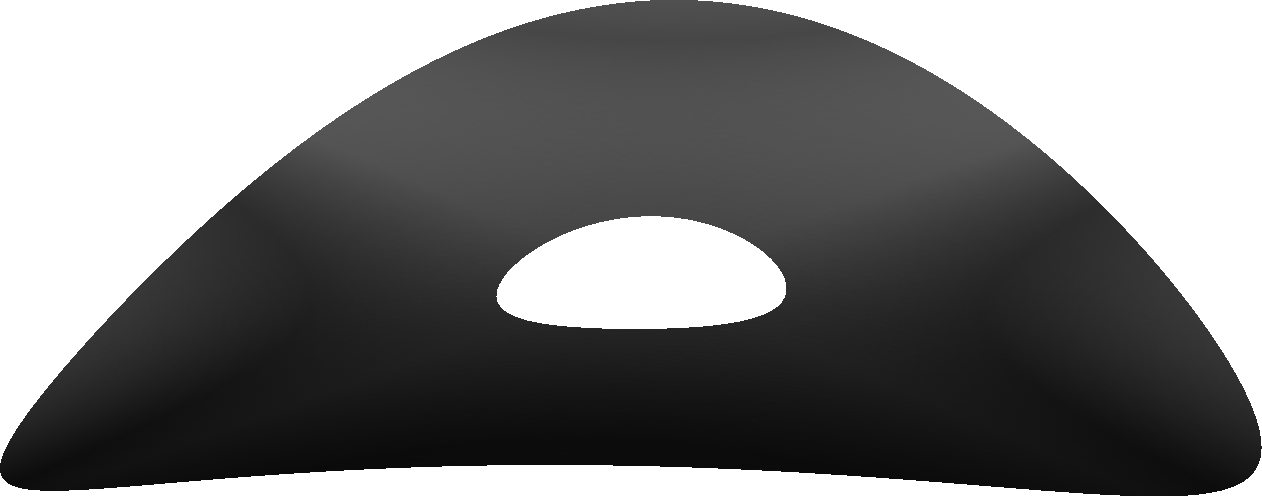
\includegraphics[width = .45\textwidth, height = .25\textwidth ]{mode5}}
\subfloat[][Modo 11]{
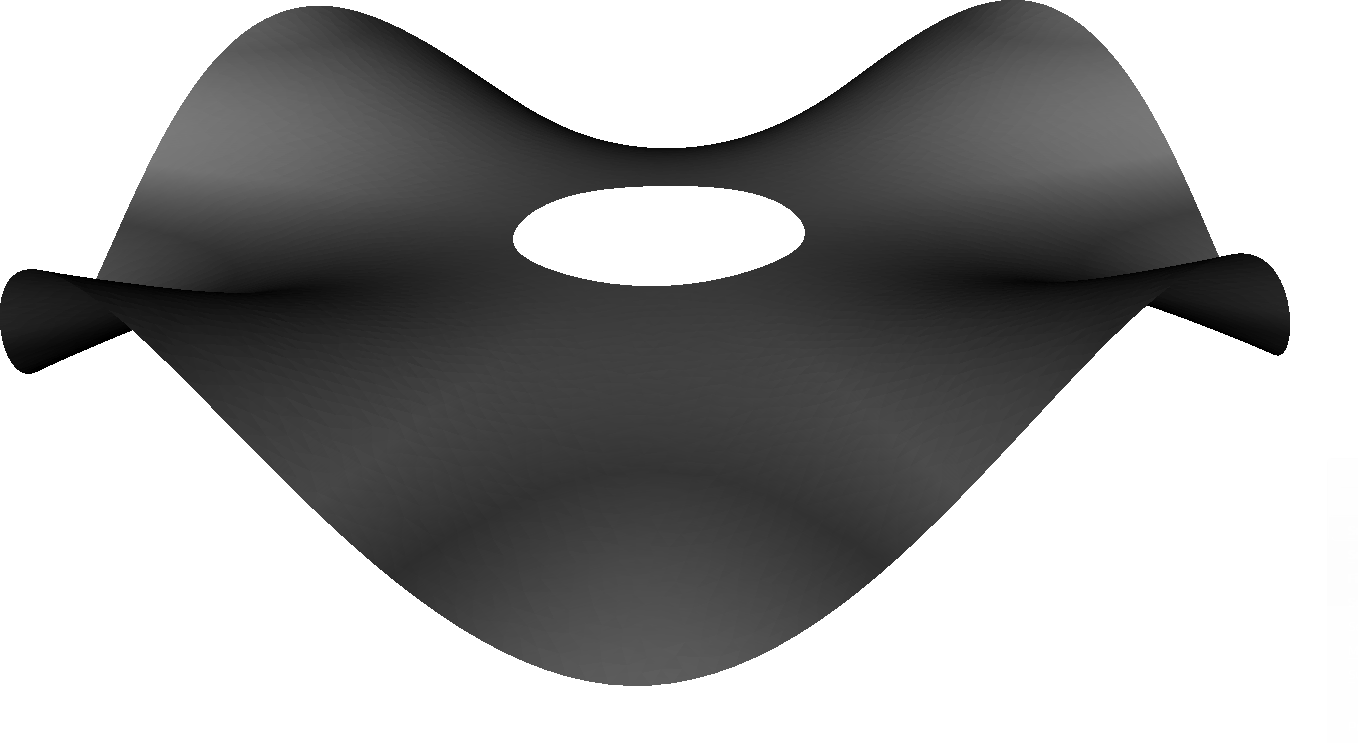
\includegraphics[width = .45\textwidth, height = .25\textwidth ]{mode11}}\\
\subfloat[][Modo 17]{
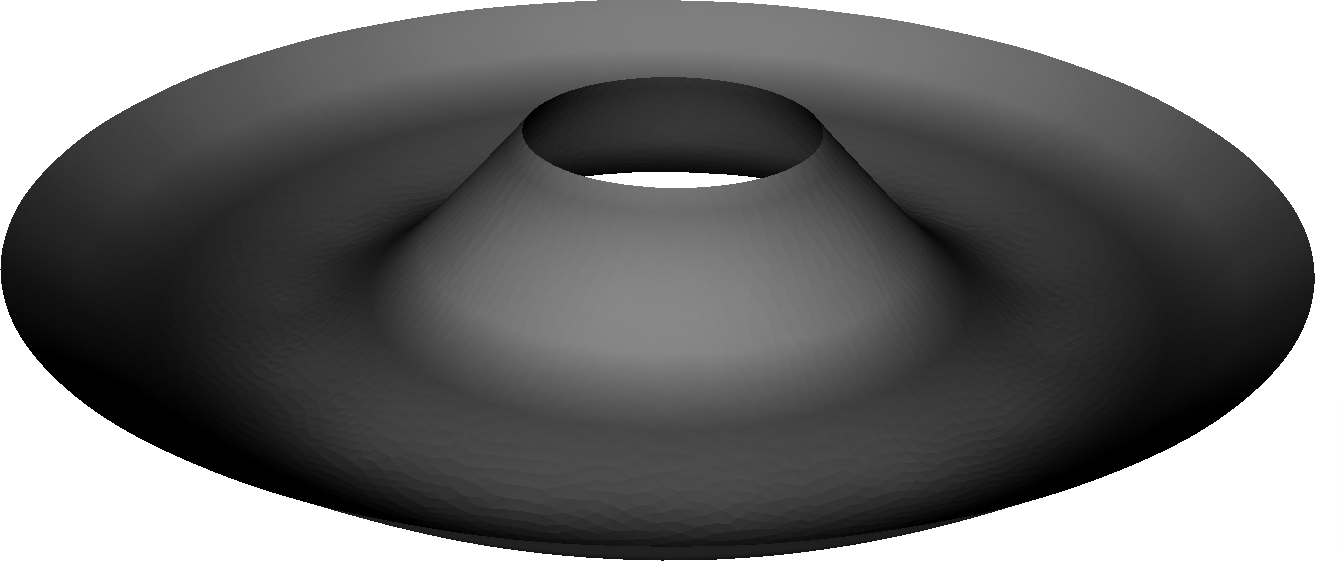
\includegraphics[width = .45\textwidth, height = .25\textwidth ]{mode17}}
\subfloat[][Modo 23]{
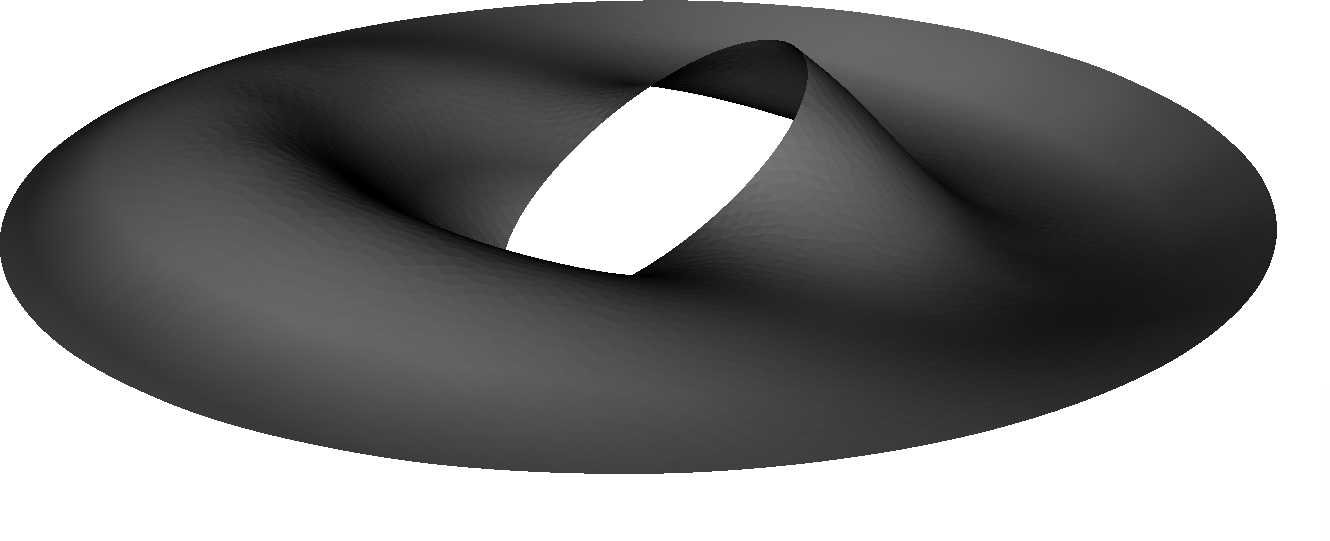
\includegraphics[width = .45\textwidth, height = .25\textwidth ]{mode23}}\\
\subfloat[][Modo 32]{
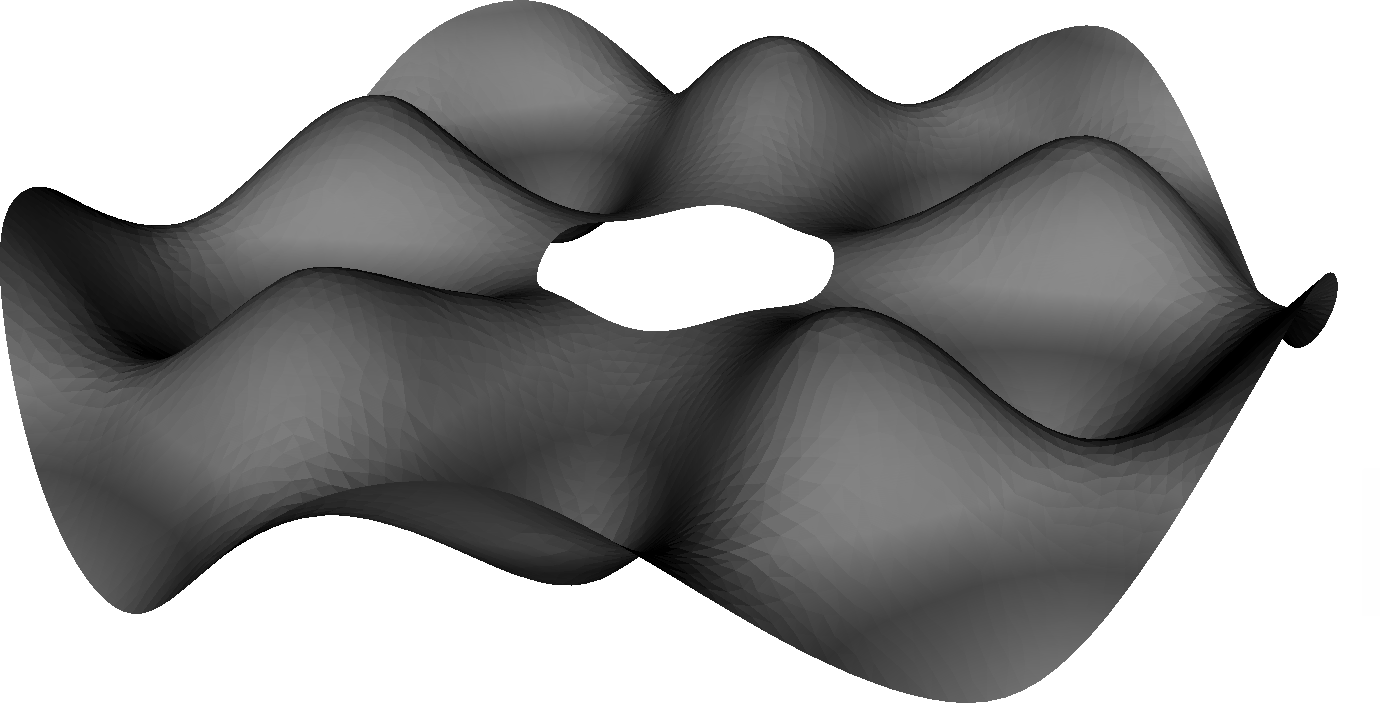
\includegraphics[width = .45\textwidth, height = .25\textwidth ]{mode32}}
\subfloat[][Modo 36]{
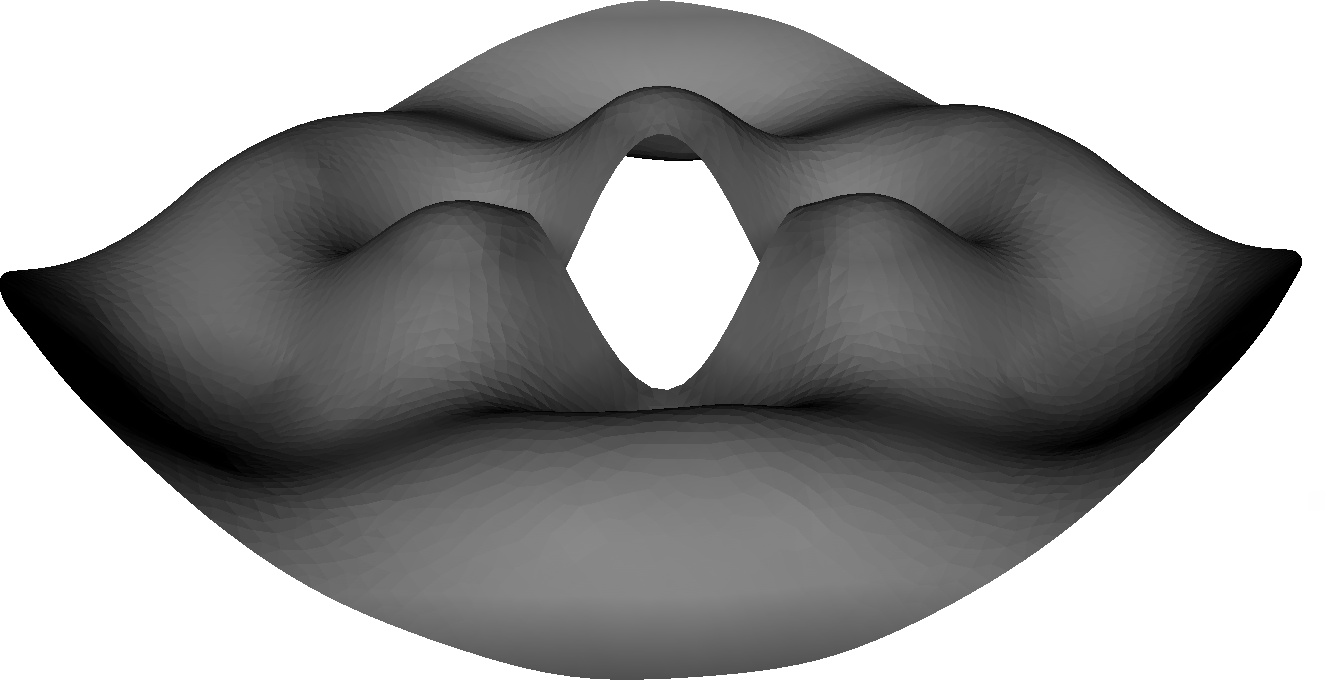
\includegraphics[width = .45\textwidth, height = .25\textwidth ]{mode36}}\\
\subfloat[][Modo 40]{
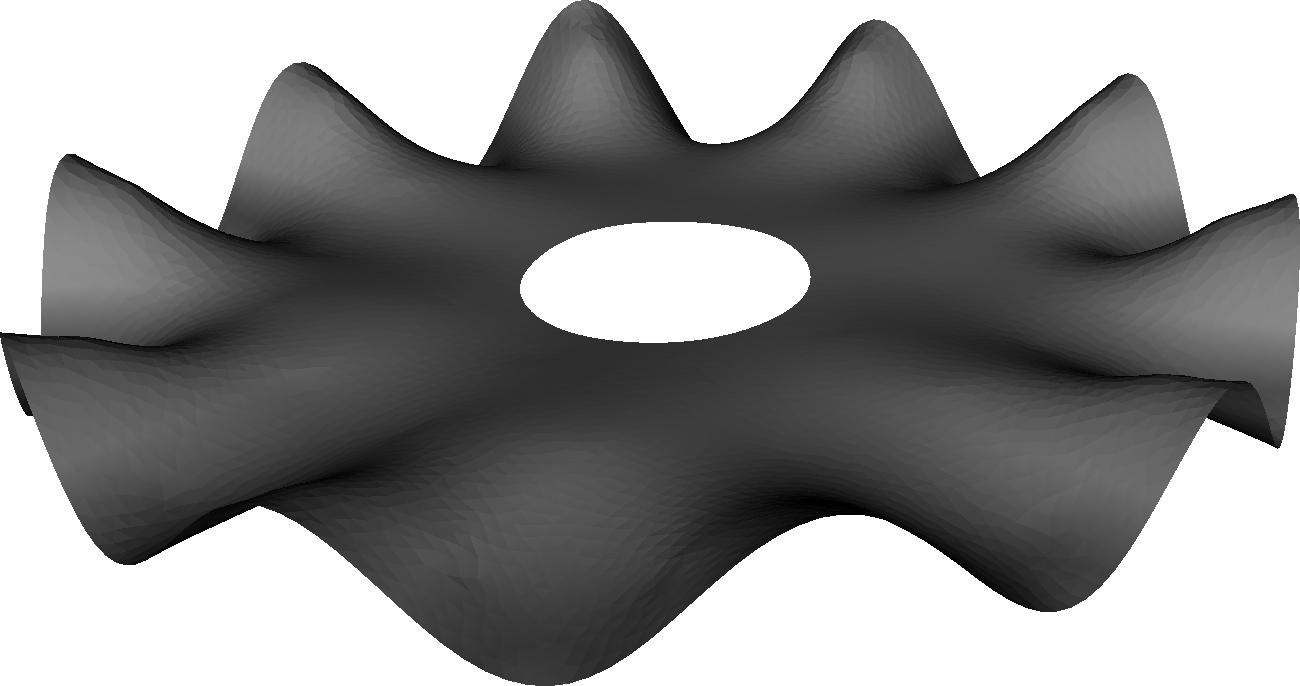
\includegraphics[width = .45\textwidth, height = .25\textwidth ]{mode40}}
\subfloat[][Modo 50]{
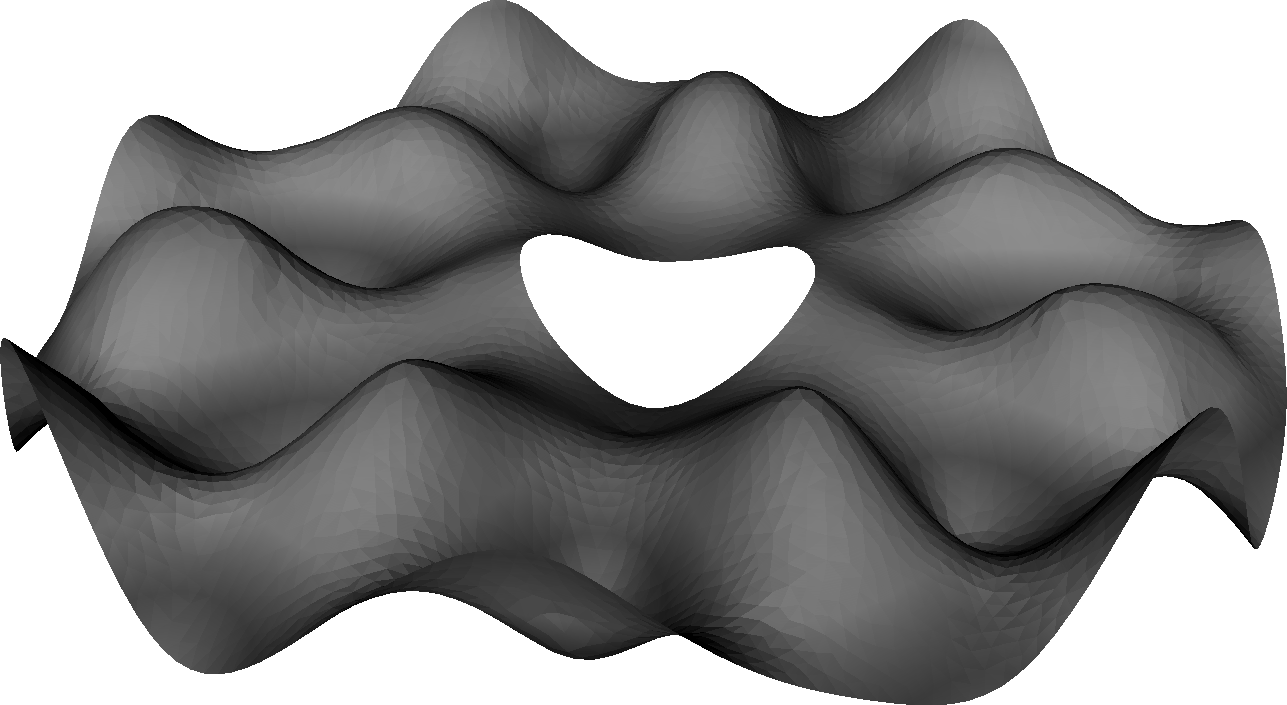
\includegraphics[width = .45\textwidth, height = .25\textwidth ]{mode50}}\\

\end{figure}


Con riferimento all'equazione \eqref{eq:7plv11} la scelta dei parametri $\alpha$ e $\beta$ per la costruzione della matrice di smorzamento mira alla rappresentazione dei contributi dissipativi strutturali e fluidodinamici. 

A basse frequenze la dissipazione è dominata dal contributo fluidodinamico.

Un fattore di smorzamento ragionevole per la sua modellazione è $\xi_1 = 0.5$ per $f_1 = 1$~Hz. Ad alta frequenza la dissipazione fluidodinamica diminuisce fortemente; sono state effettuate diverse prove per la valutazione del secondo parametro variando lo smorzamento desiderato $\xi_2$ e la frequenza $f_2$.

Provando valori conservativi ($\xi_2 = 10^{-4}$ per $f_1 = 10$~kHz) il sistema ha manifestato instabilità. \'E stata allora progressivamente aggiunta dissipazione fino ai valori che garantissero il minimo contributo dissipativo in grado di garantire la stabilità del sistema: $\xi_2 = 10^{-3}$ per $f_1 = 1$~kHz. Risolvendo il sistema lineare \eqref{eq:7plv12} si ottengono i seguenti parametri:
\begin{equation}
\label{eq:7alfabeta}
\left\{\begin{array}{l}
\alpha = 6.2832\\
\beta = 1.59\cdot 10^{-7}.\\
\end{array}\right.
\end{equation}
% !TEX encoding = UTF-8 Unicode
% !TEX TS-program = pdflatex
% !TEX root = ../Tesi.tex



%************************************************
\myChapter{Simulazione della risposta del sistema}
%************************************************
\label{chap:simulations}

Al fine di valutare la corretta implementazione della struttura, dello specchio e del sistema di controllo, il sistema viene considerato dapprima come "ideale": non sono introdotti disturbi e comportamenti non lineari, non viene simulato il reale comportamento di attuatori e sensori, l'implementazione è analogica e si suppone di avere a disposizione in ogni istante la vera misura di posizione e velocità nei punti di misura per la controreazione.

Successivamente verranno inseriti gli effetti che costituiscono fonte di disturbo e imprecisione, così da valutare le differenze nella risposta del sistema. 

\section{Test del sistema}
Per un primo test sono  state utilizzate come riferimenti alcune forme definite dai polinomi di Zernike. Questi polinomi, ortogonali fra loro, rappresentano gli elementi di una base per la rappresentazione delle aberrazioni dei fronti d'onda \citep{shannon_applied_1992}.
In un sistema di coordinate polari, possono essere costruiti grazie alle seguenti relazioni:
\begin{equation}
\label{eq:8zernike1}
Z_n^m(\rho,\theta) = 
\left\{
\begin{array}{c}
N_n^mR_n^{|m|}(\rho)\cos(m\theta) \qquad \text{per } \begin{array}{l}m \ge 0\\ 0\le\rho\le
 1\\ 0\le \theta\le 2\pi\end{array}\\
-N_n^mR_n^{|m|}(\rho)\sin(m\theta) \qquad \text{per } \begin{array}{l}m<0\\ 0\le\rho\le1\\ 0\le \theta\le 2\pi\end{array}
\end{array}\right.
\end{equation}
\begin{equation}
\label{eq:8zernike2}
N_n^m = \sqrt{\frac{2(n+1)}{1+\delta_{m=0}}}
\end{equation}
\begin{equation}
\label{eq:8zernike3}
R_n^{|m|}(\rho) = \sum_{s = 0}^{(n-|m|)/2}\frac{(-1)^s(n-s)!}{s!\left[\left(n+|m|\right)/2-s\right]\left[\left(n-|m|\right)/2-s\right]}\rho^{n-2s}
\end{equation}
Nelle formule riportate $n$ assume valori interi non negativi, $m$ varia da $-n$ a $n$ con passo 2 e $\delta_{m=0}$ è il delta di Kronecker e vale 1 per $m=0$ e $0$ per $m\neq 0$.

In Tabella \ref{tab:8zernike} sono riportati i primi 10 polinomi, nei quali $n$ varia da $0$ a 3.
\begin{table}[htb]
\centering
\caption{Elenco dei primi polinomi di Zernike}
\label{tab:8zernike}
\begin{tabular}{cccl}
\toprule
$No.$ & $n$ & $m$ & $Z_n^m(\rho,\theta)$\\
\midrule
0 & 0 &  0  & 1\\
1 & 1 &  -1 & $2\rho\sin(\theta)$\\
2 & 1 &  1  & $2\rho\cos(\theta)$\\
3 & 2 &  -2 & $\sqrt{6}\rho^2\sin(2\theta)$\\
4 & 2 &  0  & $\sqrt{3}\left(2\rho^2-1\right)$\\
5 & 2 &  2  & $\sqrt{6}\rho^2\cos(2\theta)$\\
6 & 3 &  -3 & $\sqrt{8}\rho^3\sin(3\theta)$\\
7 & 3 &  -1 & $\sqrt{8}\left(3\rho^3-2\rho\right)\sin(\theta)$\\
8 & 3 &  1  & $\sqrt{8}\left(3\rho^3-2\rho\right)\cos(\theta)$\\
9 & 3 &  3  & $\sqrt{8}\rho^3\cos(3\theta)$\\
&&&\vdots\\
\bottomrule
\end{tabular}
\end{table}


\begin{figure}[htb]
\footnotesize
\centering
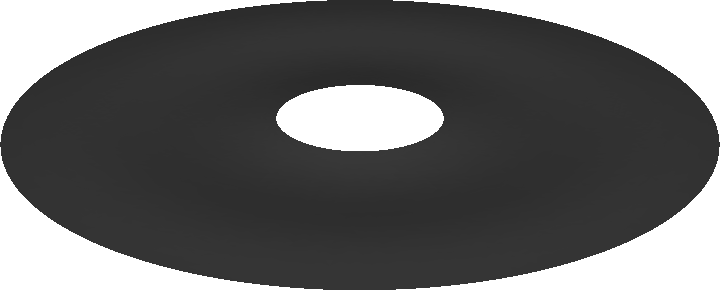
\includegraphics[width = .7\textwidth]{controlz0}
 \begin{tikzpicture}
    \begin{axis}[legend pos = south east,
    			 axis y line = left,
                 axis x line = left,
    		     width = .8\textwidth,
    		     height = .3\textheight,
                 ylabel = {$w$ (nm)}, 
                 xlabel = {$t$ (ms)}]
    \addplot[dashed, very thin, samples = 200., smooth]
    file {./Immagini/Simulations/0ref1.dat};
    \addplot[very thin, samples = 200, smooth]
    file {./Immagini/Simulations/0u1.dat};
    \addplot[dotted, samples = 200., smooth]
    file {./Immagini/Simulations/0ref1-10.dat};
    \addplot[dotted, samples = 200., smooth]
    file {./Immagini/Simulations/0ref1+10.dat};
    \legend{$r$\\$w$\\$\pm 10$ nm\\}
    \end{axis}
    \end{tikzpicture}

 \begin{tikzpicture}
    \begin{axis}[legend pos = south east,
    		     axis y line = left,
                 axis x line = left,
    		     width = .8\textwidth,
    		     height = .3\textheight,
                 ylabel = {$w$ (nm)}, 
                 xlabel = {$t$ (ms)}]
    \addplot[very thin, dashed,  samples = 200., smooth]
    file {./Immagini/Simulations/0ref2.dat};
    \addplot[very thin, samples = 200, smooth]
    file {./Immagini/Simulations/0u2.dat};
    \addplot[dotted,  samples = 200, smooth]
    file {./Immagini/Simulations/0ref2-10.dat};
    \addplot[dotted,  samples = 200., smooth]
    file {./Immagini/Simulations/0ref2+10.dat};        
    \legend{$r$\\$w$\\$\pm 10$ nm\\}
    \end{axis}
    \end{tikzpicture}

\caption{Storia temporale dello spostamento in due punti di controllo per il polinomio di Zernike n° $0$}
\label{fig:8storyzernike0}
\end{figure}


\begin{figure}[htb]
\footnotesize
\centering
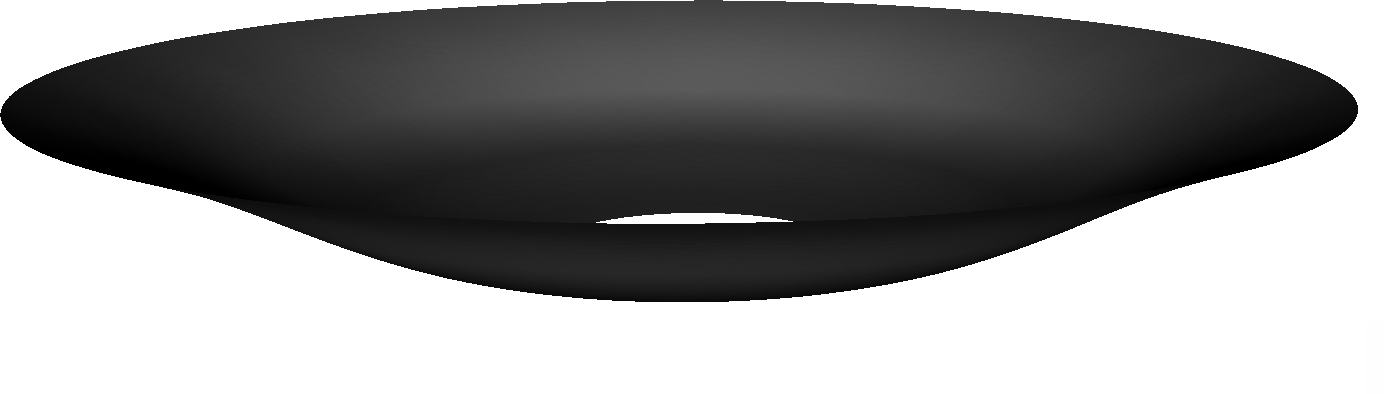
\includegraphics[width = .7\textwidth]{controlz3}

 \begin{tikzpicture}
    \begin{axis}[legend pos = south east,
    			 axis y line = left,
                 axis x line = left,
    		     width = .8\textwidth,
    		     height = .3\textheight,
                 ylabel = {$w$ (nm)}, 
                 xlabel = {$t$ (ms)}]
    \addplot[dashed, very thin, samples = 200., smooth]
    file {./Immagini/Simulations/3ref1.dat};
    \addplot[very thin, samples = 200, smooth]
    file {./Immagini/Simulations/3u1.dat};
    \addplot[dotted,  samples = 200., smooth]
    file {./Immagini/Simulations/3ref1-10.dat};
    \addplot[dotted,  samples = 200., smooth]
    file {./Immagini/Simulations/3ref1+10.dat};
    \legend{$r$\\$w$\\$\pm 10$ nm\\}
    \end{axis}
    \end{tikzpicture}

 \begin{tikzpicture}
    \begin{axis}[legend pos = north east,
    			 axis y line = left,
                 axis x line = left,
    		     width = .8\textwidth,
    		     height = .3\textheight,
                 ylabel = {$w$ (nm)}, 
                 xlabel = {$t$ (ms)}]
    \addplot[very thin, dashed,  samples = 200., smooth]
    file {./Immagini/Simulations/3ref2.dat};
    \addplot[very thin, samples = 200, smooth]
    file {./Immagini/Simulations/3u2.dat};
    \addplot[dotted, samples = 200, smooth]
    file {./Immagini/Simulations/3ref2-10.dat};
    \addplot[dotted,  samples = 200., smooth]
    file {./Immagini/Simulations/3ref2+10.dat};        
    \legend{$r$\\$w$\\$\pm 10$ nm\\}
    \end{axis}
    \end{tikzpicture}
\caption{Storia temporale dello spostamento in due punti di controllo per il 3° polinomio di Zernike}
\label{fig:8storyzernike3}
\end{figure}

\begin{figure}[htb]
\footnotesize
\centering

\includegraphics[width = .7\textwidth]{controlz9}

 \begin{tikzpicture}
    \begin{axis}[legend pos = north east,
    			 axis y line = left,
                 axis x line = left,
    		     width = .8\textwidth,
    		     height = .2\textheight,
                 ylabel = {$w$ (nm)}, 
                 xlabel = {$t$ (ms)}]
    \addplot[dashed, very thin, samples = 200., smooth]
    file {./Immagini/Simulations/9ref1.dat};
    \addplot[very thin, samples = 200, smooth]
    file {./Immagini/Simulations/9u1.dat};
    \addplot[dotted, samples = 200., smooth]
    file {./Immagini/Simulations/9ref1-10.dat};
    \addplot[dotted, samples = 200., smooth]
    file {./Immagini/Simulations/9ref1+10.dat};
    \legend{$r$\\$w$\\$\pm 10$ nm\\}
    \end{axis}
    \end{tikzpicture}

 \begin{tikzpicture}
    \begin{axis}[legend pos = south east,
                 axis y line = left,
                 axis x line = left,
    		     width = .8\textwidth,
    		     height = .3\textheight,
                 ylabel = {$w$ (nm)}, 
                 xlabel = {$t$ (ms)}]
    \addplot[very thin, dashed,  samples = 200., smooth]
    file {./Immagini/Simulations/9ref2.dat};
    \addplot[very thin, samples = 200, smooth]
    file {./Immagini/Simulations/9u2.dat};
    \addplot[dotted, samples = 200, smooth]
    file {./Immagini/Simulations/9ref2-10.dat};
    \addplot[dotted, samples = 200., smooth]
    file {./Immagini/Simulations/9ref2+10.dat};        
    \legend{$r$\\$w$\\$\pm 10$ nm\\}
    \end{axis}
    \end{tikzpicture}
\caption{Storia temporale dello spostamento in due punti di controllo per il 9° polinomio di Zernike}
\label{fig:8storyzernike9}
\end{figure}

\begin{figure}[htb]
\footnotesize
\centering
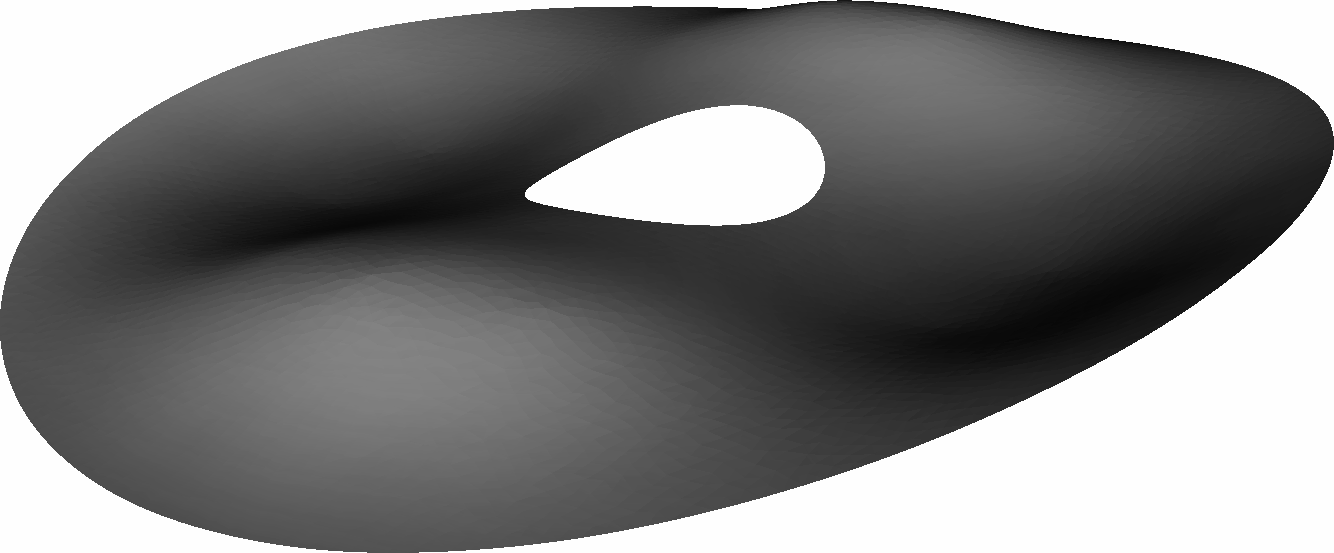
\includegraphics[width = .7\textwidth]{controlz12}

 \begin{tikzpicture}
    \begin{axis}[legend pos = south east,
    			 axis y line = left,
                 axis x line = left,
    		     width = .8\textwidth,
    		     height = .3\textheight,
                 ylabel = {$w$ (nm)}, 
                 xlabel = {$t$ (ms)}]
    \addplot[dashed, very thin, samples = 200., smooth]
    file {./Immagini/Simulations/12ref1.dat};
    \addplot[very thin, samples = 200, smooth]
    file {./Immagini/Simulations/12u1.dat};
    \addplot[dotted, samples = 200., smooth]
    file {./Immagini/Simulations/12ref1-10.dat};
    \addplot[dotted,  samples = 200., smooth]
    file {./Immagini/Simulations/12ref1+10.dat};
    \legend{$r$\\$w$\\$\pm 10$ nm\\}
    \end{axis}
    \end{tikzpicture}

 \begin{tikzpicture}
    \begin{axis}[axis y line = left,
                 axis x line = left,
    		     width = .8\textwidth,
    		     height = .3\textheight,
                 ylabel = {$w$ (nm)}, 
                 xlabel = {$t$ (ms)}]
    \addplot[very thin, dashed,  samples = 200., smooth]
    file {./Immagini/Simulations/12ref2.dat};
    \addplot[very thin, samples = 200, smooth]
    file {./Immagini/Simulations/12u2.dat};
    \addplot[dotted, samples = 200, smooth]
    file {./Immagini/Simulations/12ref2-10.dat};
    \addplot[dotted,  samples = 200., smooth]
    file {./Immagini/Simulations/12ref2+10.dat};        
    \legend{$r$\\$w$\\$\pm 10$ nm\\}
    \end{axis}
    \end{tikzpicture}
\caption{Storia temporale dello spostamento in due punti di controllo per il 12° polinomio di Zernike}
\label{fig:8storyzernike12}
\end{figure}

\begin{figure}[htb]
\footnotesize
\centering
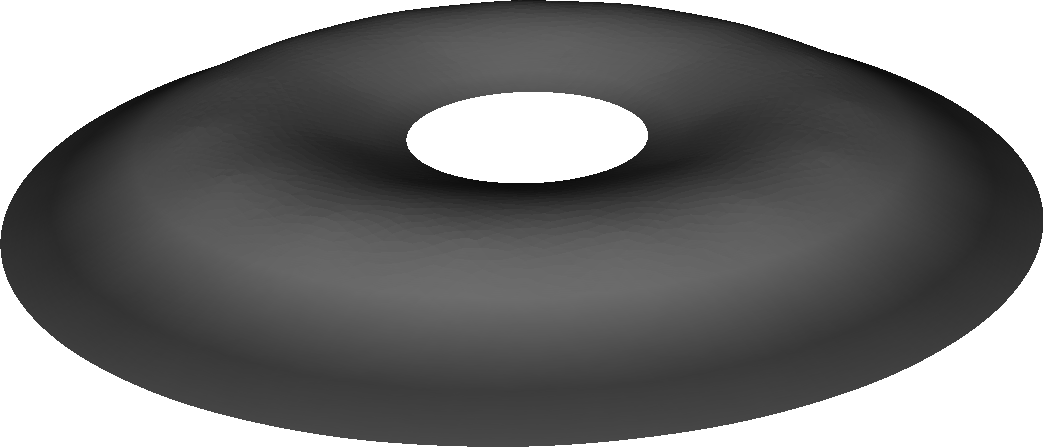
\includegraphics[width = .7\textwidth]{controlz15}

 \begin{tikzpicture}
    \begin{axis}[legend pos = north east,
    			 axis y line = left,
                 axis x line = left,
    		     width = .8\textwidth,
    		     height = .3\textheight,
                 ylabel = {$w$ (nm)}, 
                 xlabel = {$t$ (ms)}]
    \addplot[dashed, very thin, samples = 200., smooth]
    file {./Immagini/Simulations/15ref1.dat};
    \addplot[very thin, samples = 200, smooth]
    file {./Immagini/Simulations/15u1.dat};
    \addplot[dotted,  samples = 200., smooth]
    file {./Immagini/Simulations/15ref1-10.dat};
    \addplot[dotted, samples = 200., smooth]
    file {./Immagini/Simulations/15ref1+10.dat};
    \legend{$r$\\$w$\\$\pm 10$ nm\\}
    \end{axis}
    \end{tikzpicture}

 \begin{tikzpicture}
    \begin{axis}[legend pos = south east,
                 axis y line = left,
                 axis x line = left,
    		     width = .8\textwidth,
    		     height = .3\textheight,
                 ylabel = {$w$ (nm)}, 
                 xlabel = {$t$ (ms)}]
    \addplot[very thin, dashed,  samples = 200., smooth]
    file {./Immagini/Simulations/15ref2.dat};
    \addplot[very thin, samples = 200, smooth]
    file {./Immagini/Simulations/15u2.dat};
    \addplot[dotted, samples = 200, smooth]
    file {./Immagini/Simulations/15ref2-10.dat};
    \addplot[dotted, samples = 200., smooth]
    file {./Immagini/Simulations/15ref2+10.dat};        
    \legend{$r$\\$w$\\$\pm 10$ nm\\}
    \end{axis}
    \end{tikzpicture}
\caption{Storia temporale dello spostamento in due punti di controllo per il 15° polinomio di Zernike}
\label{fig:8storyzernike15}
\end{figure}

Per le simulazioni sono stati utilizzati guadagni elevati (Tabella \ref{tab:8zergains}); ciò nonostante non si manifesta instabilità nella risposta poiché il comando in anello aperto è composto da un singolo passo di un millisecondo e non sono introdotti errori o disturbi
Si può notare come indipendentemente dalle forme assunte e dagli spostamenti imposti dei singoli punti di controllo, gli errori rimangono ampiamente entro la fascia dei $\pm10$ nm, con oscillazioni assenti o di bassissima entità. Da notare la sovra-elongazione frequente al termine del raccordo, che viene recuperata dal controllo in ciclo chiuso nella fase in cui il comando è costante.

\begin{SCtable}[2][h]
\centering
\footnotesize
\begin{tabular}{ll}
\toprule
Frequenza ciclo aperto & 1 kHz\\
Frequenza ciclo chiuso & 80 kHz\\
Frequenza integrazione & 400 kHz\\
Parametri di smorzamento & $\alpha = 6.2832~\text{Hz}$\\
&$\beta=1.59\cdot10^{-7}~\text{s}$\\
Guadagno proporzionale & 100000 Kg/s$^2$\\
Guadagno derivativo & 50 Kg/s\\
Ossimoronico & Non attivo\\
\bottomrule
\end{tabular}
\label{tab:8zergains}
\caption{Parametri di controllo utilizzati per l'inseguimento delle forme di Zernike}
\end{SCtable}

\clearpage
\section{Storia temporale}
\begin{figure}[htb]
\footnotesize
\centering
\begin{tikzpicture}
    \begin{axis}[name = one,
                 legend pos = south east,
                 axis y line = left,
                 axis x line = left,
    		     width = \textwidth,
    		     height = .3\textheight,
                 ylabel = {$w$ (nm)}, 
                 xlabel = {$t$ (ms)}]
    \addplot[very thin,  samples = 200., smooth]
    file {./Immagini/Simulations2/refsmall.dat};
    \end{axis}
    \begin{axis}[
                 name=two,
                 at=(one.below south), 
                 anchor=above north,      
                 legend pos = south east,
                 axis y line = left,
                 axis x line = left,
    		     width = \textwidth,
    		     height = .3\textheight,
                 ylabel = {$w$ (nm)}, 
                 xlabel = {$t$ (ms)}]
    \addplot[very thin,  samples = 200., smooth]
    file {./Immagini/Simulations2/refzoom.dat};
    \end{axis}
    \draw[->] (4,1.8)--(5,-2);
    \draw (4,2.1) circle (.3);
\end{tikzpicture};
\caption{Storia del segnale di riferimento in un periodo di 1 secondo}
\label{fig:8refstory}
\end{figure}
In questa sezione viene valutata la risposta del sistema ad una tipica storia di comando. Il riferimento è composto da 1000 passi di comando in ciclo aperto alla frequenza di 1 kHz. Partendo dal sistema di controllo illustrato nella sezione precedente, verranno aggiunti al sistema i seguenti effetti:
\begin{itemize}
\item Simulazione del comportamento reale di sensori e attuatori;
\item Forze costanti: attrazione dei magneti di bias e forza di gravità;
\item Offset orizzontale fra i componenti degli attuatori causato da errori di montaggio e gravità;
\item Simulazione dell'elaborazione delle misure: effetto di ritardo e ricostruzione della velocità tramite schemi alle differenze finite, digitalizzazione e rumore di misura.

\end{itemize}
In Figura \ref{fig:8refstory} viene mostrata la storia in corrispondenza di un attuatore; dall'ingrandimento si possono osservare i gradini raccordati di cui è composto. 
Considerando la zona evidenziata verrà mostrato l'andamento del sistema in termini di storie temporali di posizione e velocità. 

Si sottolinea che ad ogni aggiunta di una fonte di errore la matrice di rigidezza ridotta deve essere identificata nuovamente. 

\subsection{Sistema ideale}

La prima simulazione viene effettuata utilizzando il sistema presentato nella sezione precedente. L'inseguimento è ottimo e, dopo l'assorbimento della sovra-elongazione iniziale nel corso dei primi cicli, il sistema presenta oscillazioni che restano pressoché ovunque all'interno della fascia di $\pm10$ nm, anche con guadagni relativamente bassi.

\begin{SCtable}[2][h]
\centering
\footnotesize
\begin{tabular}{lc}
\toprule
Guadagno proporzionale & 40000 Kg/s$^2$\\
Guadagno derivativo & 20 Kg/s\\
Ossimoronico & Non attivo\\
\bottomrule
\end{tabular}
\label{tab:8story0}
\caption{Parametri di controllo utilizzati per la risposta in Figura \ref{fig:8story0}}
\end{SCtable}

\begin{figure}[h]
\footnotesize
\centering
\begin{tikzpicture}
    \begin{axis}[name = one,
                 legend pos = north east,
                 axis y line = left,
                 axis x line = left,
    		     width = \textwidth,
    		     height = .2\textheight,
                 ylabel = {$w$ (nm)}, 
                 xlabel = {$t$ (ms)}]
    \addplot[dashed,very thin,  samples = 200., smooth]
    file {./Immagini/Simulations2/refzoom.dat};
    \addplot[very thin,  samples = 200., smooth]
    file {./Immagini/Simulations2/0utruezoom.dat};
    \addplot[dotted, samples = 200., smooth]
    file {./Immagini/Simulations2/refzoom+20.dat};
    \addplot[dotted,  samples = 200., smooth]
    file {./Immagini/Simulations2/refzoom-20.dat};

        \legend{$r$\\$w$\\$\pm 20$ nm\\}

    \end{axis}
    
    \begin{axis}[name = two,
                 at=(one.below south), 
                 anchor=above north,    
                 legend pos = south east,
                 axis y line = left,
                 axis x line = left,
    		     width = \textwidth,
    		     height = .2\textheight,
                 ylabel = {$w$ (nm)}, 
                 xlabel = {$t$ (ms)}]
    \addplot[dashed,very thin,  samples = 200., smooth]
    file {./Immagini/Simulations2/refsuperzoom.dat};    
    \addplot[dotted, samples = 200., smooth]
    file {./Immagini/Simulations2/refsuperzoom-20.dat};    
    \addplot[dotted,  samples = 200., smooth]
    file {./Immagini/Simulations2/refsuperzoom+20.dat};
    \addplot[very thin,  samples = 200., smooth]
    file {./Immagini/Simulations2/0utruesuperzoom.dat};
    \end{axis}
    \draw[->] (5.5,.5)--(5.5,-1.5);
    \draw (5.5,1.2) circle (.7);
\end{tikzpicture}
\caption{Risposta del sistema ideale}
\label{fig:8story0}
\end{figure}

\clearpage
\subsection{Simulazione del comportamento di sensori e attuatori}

Inserendo gli errori di attuazione e lettura dovuti alla non idealità degli elementi del sistema di controllo si ottengono alcune differenze nella simulazione della risposta; si può notare un piccolo errore sistematico di allontanamento dalla posizione di riferimento; la distanza fra la posizione assunta e quella del sistema ideale è di pochi nanometri. Questo dato indica che, sebbene l'errore dovuto a questi effetti sia presente e rilevabile, esso è relativamente basso e può essere facilmente assorbito con l'aggiunta di un controllo integrale (o ossimoronico). 
\begin{SCtable}[2][h]
\centering
\footnotesize
\begin{tabular}{lc}
\toprule
Guadagno proporzionale & 40000 Kg/s$^2$\\
Guadagno derivativo & 20 Kg/s\\
Ossimoronico & Non attivo\\
\bottomrule
\end{tabular}
\label{tab:8story1}
\caption{Parametri di controllo utilizzati per la risposta in Figura \ref{fig:8story1}}
\end{SCtable}

\begin{figure}[h]
\footnotesize
\centering
\begin{tikzpicture}
    \begin{axis}[name = one,
                 legend pos = north east,
                 axis y line = left,
                 axis x line = left,
    		     width = \textwidth,
    		     height = .2\textheight,
                 ylabel = {$w$ (nm)}, 
                 xlabel = {$t$ (ms)}]
    \addplot[dashed,very thin,  samples = 200., smooth]
    file {./Immagini/Simulations2/refzoom.dat};
    \addplot[very thin,  samples = 200., smooth]
    file {./Immagini/Simulations2/1utruezoom.dat};
    \addplot[dotted,  samples = 200., smooth]
    file {./Immagini/Simulations2/refzoom+20.dat};
    \addplot[dotted,  samples = 200., smooth]
    file {./Immagini/Simulations2/refzoom-20.dat};

        \legend{$r$\\$w$\\$\pm 20$ nm\\}

    \end{axis}
    
    \begin{axis}[name = two,
                 at=(one.below south), 
                 anchor=above north,    
                 legend pos = south east,
                 axis y line = left,
                 axis x line = left,
    		     width = \textwidth,
    		     height = .2\textheight,
                 ylabel = {$w$ (nm)}, 
                 xlabel = {$t$ (ms)}]
    \addplot[dashed,very thin,  samples = 200., smooth]
    file {./Immagini/Simulations2/refsuperzoom.dat};    
    \addplot[dotted,  samples = 200., smooth]
    file {./Immagini/Simulations2/refsuperzoom-20.dat};    
    \addplot[dotted,  samples = 200., smooth]
    file {./Immagini/Simulations2/refsuperzoom+20.dat};
    \addplot[very thin,  samples = 200., smooth]
    file {./Immagini/Simulations2/1utruesuperzoom.dat};
    \end{axis}
    \draw[->] (5.5,.5)--(5.5,-1.5);
    \draw (5.5,1.2) circle (.7);
\end{tikzpicture}
\caption{Variazione della risposta in seguito alla simulazione del comportamento di sensori e attuatori}
\label{fig:8story1}
\end{figure}


\subsection{Forze costanti}
Viene aggiunto l'effetto delle forze costanti: la gravità e le forze scambiate fra i magneti di shell e bias alla distanza nominale. Quest'ultima tuttavia varia con il movimento dei punti di controllo. Questa dipendenza si traduce nell'aggiunta della matrice di rigidezza di cui all'equazione \eqref{eq:6fc_xzalfa5}. Si considera, per la gravità, la configurazione di specchio orizzontale. La forza di gravità agisce verso il basso, mentre le forze di bias (il cui contributo è maggiore) agiscono verso l'alto.

L'aggiunta delle azioni costanti provoca un allontanamento dal riferimento; la posizione rimane comunque entro $\pm$20 nm dal riferimento, pur senza l'attivazione di un'azione integrale.
\begin{SCtable}[2][h]
\centering
\footnotesize
\begin{tabular}{lc}
\toprule
Guadagno proporzionale & 40000 Kg/s$^2$\\
Guadagno derivativo & 20 Kg/s\\
Ossimoronico & Non attivo\\
\bottomrule
\end{tabular}
\label{tab:8story2}
\caption{Parametri di controllo utilizzati per la risposta in Figura \ref{fig:8story2}}
\end{SCtable}
\begin{figure}[h]
\footnotesize
\centering
\begin{tikzpicture}
    \begin{axis}[name = one,
                 legend pos = north east,
                 axis y line = left,
                 axis x line = left,
    		     width = \textwidth,
    		     height = .2\textheight,
                 ylabel = {$w$ (nm)}, 
                 xlabel = {$t$ (ms)}]
    \addplot[dashed,very thin,  samples = 200., smooth]
    file {./Immagini/Simulations2/refzoom.dat};
    \addplot[very thin,  samples = 200., smooth]
    file {./Immagini/Simulations2/2utruezoom.dat};
    \addplot[dotted, samples = 200., smooth]
    file {./Immagini/Simulations2/refzoom+20.dat};
    \addplot[dotted, samples = 200., smooth]
    file {./Immagini/Simulations2/refzoom-20.dat};

        \legend{$r$\\$w$\\$\pm 20$ nm\\}

    \end{axis}
    
    \begin{axis}[name = two,
                 at=(one.below south), 
                 anchor=above north,    
                 legend pos = south east,
                 axis y line = left,
                 axis x line = left,
    		     width = \textwidth,
    		     height = .2\textheight,
                 ylabel = {$w$ (nm)}, 
                 xlabel = {$t$ (ms)}]
    \addplot[dashed,very thin,  samples = 200., smooth]
    file {./Immagini/Simulations2/refsuperzoom.dat};    
    \addplot[dotted, samples = 200., smooth]
    file {./Immagini/Simulations2/refsuperzoom-20.dat};    
    \addplot[dotted,  samples = 200., smooth]
    file {./Immagini/Simulations2/refsuperzoom+20.dat};
    \addplot[very thin,  samples = 200., smooth]
    file {./Immagini/Simulations2/2utruesuperzoom.dat};
    \end{axis}
    \draw[->] (5.5,.5)--(5.5,-1.5);
    \draw (5.5,1.2) circle (.7);
\end{tikzpicture}
\caption{Variazione della risposta in seguito all'introduzione di forze costanti}
\label{fig:8story2}
\end{figure}



\subsection{Offset orizzontale degli attuatori}
L'installazione dei sistemi di attuazione degli specchi comporta in genere un errore di posizionamento che causa il disallineamento tra gli elementi dell'attuatore. Inoltre le condizioni operative prevedono in genere un'orientazione non orizzontale dello specchio. La componente della forza peso parallela alla superficie dello specchio provoca un ulteriore disallineamento. Come mostrato nel Capitolo \ref{chap:ActSens}, esiste un accoppiamento tra i gradi di libertà di movimento orizzontale e di rotazione nella matrice di rigidezza magnetica.

A differenza delle tolleranze di installazione, l'effetto della gravità possiede una direzione preferenziale (identificata dalla componente della forza peso nel piano dello specchio) e dipende dall'inclinazione: maggiore è l'angolo di rotazione rispetto alla configurazione orizzontale maggiore è il disallineamento. La combinazione dei due effetti è rappresentata con una distribuzione gaussiana avente le seguenti caratteristiche (considerando la componente della forza peso diretta lungo l'asse $x$):

\begin{equation}
\label{eq:8offset}
\left\{
\begin{array}{l}  
\mu_x = 0.7 \text{ mm}\\
\mu_y = 0.0 \text{ mm}\\
\sigma = 0.3\text{ mm}\\
\sigma_x = \sigma_y = \sigma
\end{array}\right.
\end{equation}                                            

In Figura \ref{fig:8offset} sono mostrate le deviazioni ottenute per il caso in analisi per gli attuatori considerati. L'angolo considerato per il calcolo della forza peso è $\gamma=45\degree$.

\begin{figure}[htb]
\centering
\caption{Disallineamento degli attuatori in una porzione dello specchio (in grigio la posizione nominale, in rosso il disallineamento)}
\label{fig:8offset}
\resizebox{.8\textwidth}{!}{
\begin{tikzpicture}
\filldraw[->, very thin, fill =  black!20!white](  7.898990000000000e-03*100 ,  1.053990000000000e-01*100) circle(0.0005*100);
\filldraw[->, very thin, fill =  black!20!white](  6.590000000000000e-02*100 ,  8.263600000000000e-02*100) circle(0.0005*100);
\filldraw[->, very thin, fill =  black!20!white](  8.733000000000002e-02*100 ,  5.954090000000000e-02*100) circle(0.0005*100);
\filldraw[->, very thin, fill =  black!20!white](  1.010000000000000e-01*100 ,  3.115400000000000e-02*100) circle(0.0005*100);
\filldraw[->, very thin, fill =  black!20!white](  6.833989999999998e-02*100 ,  3.042690000000000e-02*100) circle(0.0005*100);
\filldraw[->, very thin, fill =  black!20!white](  2.311690000000000e-02*100 ,  7.114600000000000e-02*100) circle(0.0005*100);
\filldraw[->, very thin, fill =  black!20!white](  5.005600000000000e-02*100 ,  5.559290000000000e-02*100) circle(0.0005*100);
\filldraw[->, very thin, fill =  black!20!white](  4.390390000000000e-02*100 ,                      0*100) circle(0.0005*100);
\filldraw[->, very thin, fill =  black!20!white](  7.623989999999999e-03*100 ,  4.323690000000000e-02*100) circle(0.0005*100);
\filldraw[->, very thin, fill =  black!20!white](  3.363200000000000e-02*100 ,  2.822100000000000e-02*100) circle(0.0005*100);
\filldraw[->, very thin, fill =  black!20!white](  1.057000000000000e-01*100 ,                      0*100) circle(0.0005*100);
\filldraw[->, very thin, fill =  black!20!white](  7.480689999999998e-02*100 ,                      0*100) circle(0.0005*100);
\filldraw[->, very thin, fill =  black!20!white](  3.861490000000000e-02*100 ,  9.839000000000001e-02*100) circle(0.0005*100);

\filldraw[->, very thin, fill = red]( 7.865019561261639e-03*100  ,  1.050932159541108e-01*100) circle(0.0005*100);
\filldraw[->, very thin, fill = red]( 6.709983686389048e-02*100  ,  8.315960623944971e-02*100) circle(0.0005*100);
\filldraw[->, very thin, fill = red]( 8.827367016204216e-02*100  ,  5.926128332093865e-02*100) circle(0.0005*100);
\filldraw[->, very thin, fill = red]( 1.017689602173930e-01*100  ,  3.095936417421868e-02*100) circle(0.0005*100);
\filldraw[->, very thin, fill = red]( 6.866844823238719e-02*100  ,  3.063964490779994e-02*100) circle(0.0005*100);
\filldraw[->, very thin, fill = red]( 2.322242002294483e-02*100  ,  7.109531749272614e-02*100) circle(0.0005*100);
\filldraw[->, very thin, fill = red]( 5.094482311768826e-02*100  ,  5.542165882274243e-02*100) circle(0.0005*100);
\filldraw[->, very thin, fill = red]( 4.445267401521948e-02*100  ,  8.359904019002389e-05*100) circle(0.0005*100);
\filldraw[->, very thin, fill = red]( 8.020215484891013e-03*100  ,  4.263401314266086e-02*100) circle(0.0005*100);
\filldraw[->, very thin, fill = red]( 3.421273209079292e-02*100  ,  2.847608596171483e-02*100) circle(0.0005*100);
\filldraw[->, very thin, fill = red]( 1.062160284583974e-01*100  , -2.048105529875691e-04*100) circle(0.0005*100);
\filldraw[->, very thin, fill = red]( 7.579406394721812e-02*100  ,  1.283680059322352e-04*100) circle(0.0005*100);
\filldraw[->, very thin, fill = red]( 3.914655134488187e-02*100  ,  9.812199694095361e-02*100) circle(0.0005*100);

\tdplotdrawarc[very thin]{(0,0)}{0.12*100}{0}{90}{}{}
\tdplotdrawarc[very thin]{(0,0)}{0.05688/2*100}{0}{90}{}{}
\draw[very thin, dashed] (0.05688/2*100,0)--(0.12*100,0);
\draw[very thin,dashed] (0,0.05688/2*100)--(0,0.12*100);
\end{tikzpicture}}
\end{figure}

Come si può osservare in Figura \ref{fig:8story3} il disallineamento provoca la deriva della posizione rispetto al riferimento che va ben oltre la tolleranza di riferimento di $\pm 20$ nm. Fra gli effetti di disturbo dovuti al funzionamento non ideale tra sensori e attuatori questo effetto è predominante.\\

\begin{SCtable}[2][h]
\centering
\footnotesize
\begin{tabular}{lc}
\toprule
Guadagno proporzionale & 40000 Kg/s$^2$\\
Guadagno derivativo & 20 Kg/s\\
Ossimoronico & Non attivo\\
\bottomrule
\end{tabular}
\label{tab:8story3}
\caption{Parametri di controllo utilizzati per la risposta in Figura \ref{fig:8story3}}
\end{SCtable}
\begin{figure}[h]
\footnotesize
\centering
\begin{tikzpicture}
    \begin{axis}[name = one,
                 axis y line = left,
                 axis x line = left,
    		     width = \textwidth,
    		     height = .2\textheight,
                 ylabel = {$w$ (nm)}, 
                 xlabel = {$t$ (ms)}]
    \addplot[dashed,very thin,  samples = 200., smooth]
    file {./Immagini/Simulations2/refzoom.dat};
    \addplot[very thin,  samples = 200., smooth]
    file {./Immagini/Simulations2/3utruezoom.dat};
    \addplot[dotted,  samples = 200., smooth]
    file {./Immagini/Simulations2/refzoom+20.dat};
    \addplot[dotted, samples = 200., smooth]
    file {./Immagini/Simulations2/refzoom-20.dat};

    \end{axis}
\end{tikzpicture}
\caption{Variazione della risposta in seguito all'introduzione di un disallineamento negli attuatori}
\label{fig:8story3}
\end{figure}

A causa dell'effetto di deriva si rileva la necessità di introdurre un controllo integrale. Per recuperare il tracciamento è stato pertanto attivato il contributo ossimoronico, finora non attivo (Figura \ref{fig:8story3bis}). 

\begin{SCtable}[2][h]
\centering
\footnotesize
\begin{tabular}{lc}
\toprule
Guadagno proporzionale & 40000 Kg/s$^2$\\
Guadagno derivativo & 20 Kg/s\\
Ossimoronico & Attivo\\
\bottomrule
\end{tabular}
\caption{Parametri di controllo utilizzati per la risposta in Figura \ref{fig:8story3bis}}
\label{tab:8story2bis}
\end{SCtable}
\begin{figure}[h]
\footnotesize
\centering
\begin{tikzpicture}
    \begin{axis}[name = one,
                 legend pos = north east,
                 axis y line = left,
                 axis x line = left,
    		     width = \textwidth,
    		     height = .2\textheight,
                 ylabel = {$w$ (nm)}, 
                 xlabel = {$t$ (ms)}]
    \addplot[dashed,very thin,  samples = 200., smooth]
    file {./Immagini/Simulations2/refzoom.dat};
    \addplot[very thin,  samples = 200., smooth]
    file {./Immagini/Simulations2/3_bis_utruezoom.dat};
    \addplot[dotted,  samples = 200., smooth]
    file {./Immagini/Simulations2/refzoom+20.dat};
    \addplot[dotted, samples = 200., smooth]
    file {./Immagini/Simulations2/refzoom-20.dat};

        \legend{$r$\\$w$\\$\pm 20$ nm\\}

    \end{axis}
    
    \begin{axis}[name = two,
                 at=(one.below south), 
                 anchor=above north,    
                 legend pos = south east,
                 axis y line = left,
                 axis x line = left,
    		     width = \textwidth,
    		     height = .2\textheight,
                 ylabel = {$w$ (nm)}, 
                 xlabel = {$t$ (ms)}]
    \addplot[dashed,very thin,  samples = 200., smooth]
    file {./Immagini/Simulations2/refsuperzoom.dat};    
    \addplot[dotted, samples = 200., smooth]
    file {./Immagini/Simulations2/refsuperzoom-20.dat};    
    \addplot[dotted, samples = 200., smooth]
    file {./Immagini/Simulations2/refsuperzoom+20.dat};
    \addplot[very thin,  samples = 200., smooth]
    file {./Immagini/Simulations2/3_bis_utruesuperzoom.dat};
    \end{axis}
    \draw[->] (5.5,.5)--(5.5,-1.5);
    \draw (5.5,1.2) circle (.7);
\end{tikzpicture}
\caption{Variazione della risposta in seguito all'introduzione di un disallineamento negli attuatori dopo l'attivazione del contributo ossimoronico}
\label{fig:8story3bis}
\end{figure}
L'introduzione del contributo ossimoronico permette l'assorbimento della deriva del sistema, con lo scotto di un aumento dell'ampiezza delle oscillazioni, che comunque restano all'interno della fascia di riferimento.
\clearpage

\subsection{Digitalizzazione}
Come ultima fonte di disturbo è stata aggiunta la simulazione del sistema di acquisizione, elaborazione e attuazione. Di seguito sono elencate le caratteristiche utilizzate per la sua modellazione. I disturbi di digitalizzazione e gli schemi di ricostruzione delle quantità misurate comportano l'introduzione di un notevole errore e, soprattutto, cambiano le caratteristiche di stabilità e robustezza del sistema di controllo.

\begin{figure}[h]
\caption{Circuito del sensore}
\label{ciao}
\centering
\begin{overpic}[width=0.6\textwidth]{circuito}
\put(18,50){$C_{stray}$}
\put(50,50){$C_{ref}$}
\put(70,17){$V_{out}$}
\put(20,25){$C_{sens}$}
\put(10,20){$V_{ref}$}
\end{overpic}
\end{figure}
Il controllore digitale è così strutturato \citep{manettiphd}:
\begin{itemize}
\item La capacità è letta analogicamente attraverso il circuito mostrato in Figura \ref{ciao}; la tensione letta $V_{out}$ viene convertita in un numero intero a 16 bit. La relazione fra la tensione e la capacità del sensore $C_{sens}$ è espressa dalla seguente formula:
\begin{equation}
\label{eq:8circuito}
V_{out} = \frac{V_{ref}}{C_{ref}}\left(C_{sens}+C_{stray}\right),
\end{equation}
dove $V_{ref}$ è la tensione di alimentazione (pari a 1 V), $C_{ref}$ e $C_{stray}$ sono capacità dai seguenti valori nominali:
\begin{equation}
\label{eq:8circuito2}
\begin{array}{l}
C_{ref} = 39\text{ pF}\\
C_{stray} = 3.9 \text{ pF}.
\end{array}
\end{equation}

\item Alla misura digitale viene introdotto un errore in bit correlato al valore di capacità letto; l'errore, ottenuto tramite la correlazione di dati sperimentali, è rappresentato con una distribuzione di probabilità gaussiana a media nulla la cui deviazione standard dipende dal valore digitale della tensione letta \citep{manettiphd}. La relazione è stata ottenuta interpolando andamenti ottenuti da stime empiriche \citep{manettiphd}::
\begin{equation}
\label{eq:8circuito3}
\sigma = 1.1+2.78\cdot 10^{-24} V_{dig}^5.
\end{equation}
\item Il controllore agisce sulla base della misura effettuata al passo precedente in ciclo chiuso; per la ricostruzione della velocità si utilizza uno schema alle differenze finite del primo ordine utilizzando le letture di posizione dei due passi precedenti:
\begin{align}
\label{eq:8circuito4}
\T{F_{cl_{k}}} = \TT{G_p}\left[\T{r}(t_k)-\tilde{\T{w}}_{k-1}\right]+ \TT{G_d}\left[\dot{\T{r}}(t_k)-\frac{\tilde{\T{w}}_{k-1}-\tilde{\T{w}}_{k-2}}{\Delta t}\right].
\end{align}
\item I circuiti di attuazione e misura sono realizzati in modulazione di ampiezza. Questa configurazione comporta il filtraggio delle posizioni misurate e delle forze applicate; per la sua rappresentazione è stato costruito un filtro passa-basso del primo ordine. Il polo per il sensore capacitivo è posto ad una frequenza $f_{sen} = 40\text{ kHz}$, mentre per il circuito d'attuazione la frequenza è $f_{act} = 25\text{ kHz}$:

\begin{align}
\label{eq:8circuito5.0}
C_f(s) = \frac{1}{1+s/(2 \pi f_{sen})} C(s)\\
\label{eq:8circuito5.1}
\T{F}_f(s) = \frac{1}{1+s/(2\pi f_{act})} \T{F}(s).\\
\end{align}

\end{itemize}
\begin{SCtable}[2][h]
\centering
\footnotesize
\begin{tabular}{lc}
\toprule
Guadagno proporzionale & 20000 Kg/s$^2$\\
Guadagno derivativo & 10 Kg/s\\
Ossimoronico & Attivo\\
$f_T$ filtro sensore & 40 kHz\\
$f_T$ filtro attuatore & 25 kHz\\
\bottomrule
\end{tabular}
\label{tab:8story4}
\caption{Parametri di controllo utilizzati per la risposta in Figura \ref{fig:8story4}}
\end{SCtable}
\begin{figure}[ht]
\footnotesize
\centering
\begin{tikzpicture}
    \begin{axis}[name = one,
                 legend pos = north east,
                 axis y line = left,
                 axis x line = left,
    		     width = \textwidth,
    		     height = .2\textheight,
                 ylabel = {$w$ (nm)}, 
                 xlabel = {$t$ (ms)}]
    \addplot[dashed,very thin,  samples = 200., smooth]
    file {./Immagini/Simulations2/refzoom.dat};
    \addplot[very thin,  samples = 200., smooth]
    file {./Immagini/Simulations2/4utruezoom.dat};
    \addplot[dotted,  samples = 200., smooth]
    file {./Immagini/Simulations2/refzoom+20.dat};
    \addplot[dotted,  samples = 200., smooth]
    file {./Immagini/Simulations2/refzoom-20.dat};

        \legend{$r$\\$w$\\$\pm 20$ nm\\}

    \end{axis}
    
    \begin{axis}[name = two,
                 at=(one.below south), 
                 anchor=above north,    
                 legend pos = south east,
                 axis y line = left,
                 axis x line = left,
    		     width = \textwidth,
    		     height = .2\textheight,
                 ylabel = {$w$ (nm)}, 
                 xlabel = {$t$ (ms)}]
    \addplot[dashed,very thin,  samples = 200., smooth]
    file {./Immagini/Simulations2/refsuperzoom.dat};    
    \addplot[dotted,  samples = 200., smooth]
    file {./Immagini/Simulations2/refsuperzoom-20.dat};    
    \addplot[dotted,  samples = 200., smooth]
    file {./Immagini/Simulations2/refsuperzoom+20.dat};
    \addplot[very thin,  samples = 200., smooth]
    file {./Immagini/Simulations2/4utruesuperzoom.dat};
    \end{axis}
    \draw[->] (5.5,.5)--(5.5,-1.5);
    \draw (5.5,1.2) circle (.7);
\end{tikzpicture}
\caption{Variazione della risposta in seguito all'introduzione della digitalizzazione}
\label{fig:8story4}
\end{figure}
L'introduzione dell'errore di digitalizzazione ha causato l'instabilizzazione del sistema. Per questo si è reso necessario un abbassamento dei guadagni, con conseguente diminuzione delle prestazioni generali del sistema (Figura \ref{fig:8story4}). In questa configurazione il contributo ossimoronico (che negli specchi attualmente operativi non è implementato ed è sostituito da un contributo integrale in ciclo chiuso) è fondamentale per evitare la deriva della posizione dello specchio, che resta entro la fascia di riferimento $\pm20$ nm.


Per un'analisi della causa dell'instabilità che ha reso necessario l'abbassamento dei guadagni, è utile osservare l'andamento della posizione in un singolo passo di controllo in anello aperto. Per questo è stata effettuata un'analisi di risposta senza forze costanti e disallineamenti, in modo da identificare il contributo della sola digitalizzazione.
In Figura \ref{fig:81step} è mostrato un confronto fra posizioni e velocità vere e misurate. Si può notare che, mentre lo spostamento misurato ben approssima quello reale ai fini della parte proporzionale del controllo in ciclo chiuso, la velocità ottenuta per differenze finite mostra un andamento altalenante che approssima malamente il reale andamento delle velocità. A causa dell'elevata frequenza delle oscillazioni, anche schemi di ricostruzione alle differenze finite di ordini più elevati portano a risultati simili. 

\begin{figure}[ht]
\footnotesize
\centering
\begin{tikzpicture}
    \begin{axis}[name = one,
                 legend pos = south east,
                 axis y line = left,
                 axis x line = left,
    		     width = \textwidth,
    		     height = .2\textheight,
                 ylabel = {$w$ (nm)}, 
                 xlabel = {$t$ (ms)}]
    \addplot[dashed,very thin,  samples = 200., smooth]
    file {./Immagini/Simulations3/refgigazoom.dat};
    \addplot[very thin,  samples = 200., smooth]
    file {./Immagini/Simulations3/5utruegigazoom.dat};
        \addplot[mark = *, dashed, very thin,  samples = 200., smooth]
    file {./Immagini/Simulations3/5ugigazoom.dat};
    \addplot[dotted, samples = 200., smooth]
    file {./Immagini/Simulations3/refgigazoom+20.dat};
    \addplot[dotted,  samples = 200., smooth]
    file {./Immagini/Simulations3/refgigazoom-20.dat};

        \legend{$r$\\$w$\\$\tilde{w}$\\$\pm 20$ nm\\}

    \end{axis}
    
    \begin{axis}[name = two,
                 at=(one.below south), 
                 anchor=above north,    
                 legend pos = south east,
                 axis y line = left,
                 axis x line = left,
    		     width = \textwidth,
    		     height = .2\textheight,
                 ylabel = {$\dot{w}$ (mm/s)}, 
                 xlabel = {$t$ (ms)}]
    \addplot[dashed,very thin,  samples = 200., smooth]
    file {./Immagini/Simulations3/refdgigazoom.dat};    
    \addplot[very thin,  samples = 200., smooth]
    file {./Immagini/Simulations3/5udtruegigazoom.dat};    
    \addplot[mark = *, dashed, very thin,  samples = 200., smooth]
    file {./Immagini/Simulations3/5udgigazoom.dat};
    
            \legend{$\dot{r}$\\$\dot{w}$\\$\dot{\tilde{w}}$\\}
   \end{axis}
   
   
\end{tikzpicture}
\caption{Dettaglio sull'azione di misura in un passo temporale di 1 ms (differenze finite)}
\label{fig:81step}
\end{figure}

L'errore nella ricostruzione delle derivate assume un ruolo cruciale: se per un ciclo di controllo la velocità letta ha segno opposto alla velocità reale, la componente derivativa dell'azione di controllo introduce energia nel sistema anziché dissiparla. Questo è il principale fattore che pone un limite ai guadagni derivativi utilizzabili, poiché a guadagni elevati il sistema diviene presto instabile a causa della continua immissione di energia. 

Dall'analisi effettuata, risulta che soltanto per il 35\% delle velocità ricostruite il segno è concorde con la velocità vera. Per questo, nella Sezione \ref{sec:recons} sono state valutate alcune strategie alternative di ricostruzione della velocità.

\section{Strategie alternative di ricostruzione della velocità}
\label{sec:recons}
\subsection{Differenze finite sulla posizione filtrata}
Una prima alternativa all'utilizzo diretto delle differenze finite consiste nel filtraggio delle posizioni lette, utilizzando un filtro digitale del primo ordine che opera alla frequenza di controllo; la pulsazione di taglio è un parametro di scelta per la scelta di un compromesso fra il tracciamento corretto dei segnali a bassa frequenza e lo sfasamento implicito nell'applicazione del filtro stesso. Allargando la banda diminuiscono gli effetti di filtraggio; d'altro canto, restringendola aumenta lo sfasamento introdotto. Dalle prove effettuate si è riscontrata stabilità per il sistema con frequenze variabili intorno ai 10 kHz.

Il filtro è digitale e lavora alla frequenza di controllo in ciclo chiuso ($80$ kHz) e assume la seguente forma:
\begin{equation}
\label{eq:8filtro1}
w^f_{k+1} = a w^f_{k}+(1-a)\tilde{w}_k,
\end{equation}
dove $w^f$ è lo stato utilizzato per la ricostruzione della velocità tramite differenze finite, $\tilde{w}$ è , come di consueto, lo spostamento misurato e $a$ è il parametro (dipendente dalla frequenza di taglio scelta) che regola le proprietà del filtro; a maggiore $a$ corrisponde una frequenza di taglio minore. Si può operare direttamente su tale parametro per la regolazione del filtro.\\

Per la retroazione proporzionale si preferisce, a dispetto del rumore ma a favore della stabilità,  utilizzare direttamente lo spostamento misurato; l'azione derivativa sfrutta invece le differenze finite sui valori filtrati dello stesso.

\begin{SCtable}[2][h]
\centering
\footnotesize
\begin{tabular}{lc}
\toprule
Guadagno proporzionale & 20000 Kg/s$^2$\\
Guadagno derivativo & 15 Kg/s\\
Ossimoronico & Attivo\\
$f_T$ filtro sensore & 40 kHz\\
$f_T$ filtro attuatore & 25 kHz\\
$f_T$ filtro per ricostruzione & 10 kHz\\
\bottomrule
\end{tabular}
\label{tab:8story5}
\caption{Parametri di controllo utilizzati per la risposta in Figura \ref{fig:81step.1}}
\end{SCtable}
\begin{figure}[htb]
\footnotesize
\centering
\begin{tikzpicture}
    \begin{axis}[name = two,
                 at=(one.below south), 
                 anchor=above north,    
                 legend pos = north east,
                 axis y line = left,
                 axis x line = left,
    		     width = \textwidth,
    		     height = .2\textheight,
                 ylabel = {$\dot{w}$ (mm/s)}, 
                 xlabel = {$t$ (ms)}]
    \addplot[dashed,very thin,  samples = 200., smooth]
    file {./Immagini/Simulations3/refdgigazoom.dat};    
    \addplot[very thin,  samples = 200., smooth]
    file {./Immagini/Simulations3/6udtruegigazoom.dat};    
    \addplot[mark = *, dashed,  very thin,  samples = 200., smooth]
    file {./Immagini/Simulations3/6udgigazoom.dat};
    
            \legend{$\dot{r}$\\$\dot{w}$\\$\dot{\tilde{w}}$\\}
   \end{axis}
   
   
\end{tikzpicture}
\caption{Dettaglio sull'azione di misura in un passo temporale di 1 ms (differenze finite sulla posizione filtrata)}
\label{fig:81step.1}
\end{figure}
Dai risultati si può osservare quanto la velocità risulti meglio interpretata: le ampiezze sono paragonabili e gli errori di segno sono notevolmente diminuiti. La percentuale di valori correttamente interpretati, sale al 55\%. Questo incremento è fondamentale per la robustezza del sistema in quanto, in mancanza di precisione, se il numero di segni corretti è almeno pari al 50\% del totale, il contributo complessivo del sistema di controllo sarà sempre di dissipazione.

 Inoltre la deviazione standard della differenza tra velocità ricostruita e reale è passato da circa 5.5 mm/s a 1.5 mm/s. 
Ne consegue un notevole miglioramento della stabilità del sistema.

\subsection{Il filtro come osservatore di stato}
Un'interpretazione dello schema \eqref{eq:8filtro1} permette di giustificare l'incremento della qualità della velocità ricostruita e offre spunti per l'applicazione di schemi più raffinati. Si scriva il seguente sistema agli stati, basato sull'approssimazione dello spostamento reale $w$ come quantità costante a tratti soggetta ad un disturbo $d$ e da un rumore di misura $r$:
\begin{equation}
\label{eq:8filtro2}
\left\{
\begin{array}{l}
\dot{w} = 0+d\\
\tilde{w} = w +r.
\end{array}\right.
\end{equation}

Si scelga come disturbo $d$ l'attuale velocità del sistema $v^w$. Così facendo, la banale equazione $\dot{w} = v^w$ viene reinterpretata, identificando con $v^w$ un disturbo che agisce su un sistema in cui $\dot{w}=0$:

\begin{equation}
\label{eq:8filtro3}
\left\{
\begin{array}{l}
\dot{w} = 0+v^w\\
\tilde{w} = w +r.
\end{array}\right.
\end{equation}

Il sistema, discretizzato a tempo $\Delta t$ assume la forma:
\begin{equation}
\label{eq:8filtro4}
\left\{
\begin{array}{l}
w_{k+1} = w_k+\Delta t ~v^w_k\\
\tilde{w}_k = w_k +r_k.
\end{array}\right.
\end{equation}

Si può osservare come la prima delle equazioni \eqref{eq:8filtro4} altro non è che l'equazione di ricostruzione della velocità tramite lo schema delle differenze finite all'indietro di primo ordine:
\begin{equation}
\label{eq:8filtro5}
v^w_k = \frac{w_{k+1}-w_k}{\Delta t}
\end{equation}

Applicando al filtro un osservatore alla Kalman, si ha:
\begin{equation}
\label{eq:8filtro6}
\left\{
\begin{array}{l}
w_{k+1} = w_k+L(\tilde{w}_k-w_k)+\Delta t~ v^w_k\\
\tilde{w}_k = w_k +r_k
\end{array}\right.
\end{equation}

\begin{equation}
\label{eq:8filtro7}
\left\{
\begin{array}{l}
w_{k+1} = (1-L)w_k+L\tilde{w}_k+\Delta t~ v^w_k\\
\tilde{w}_k = w_k +r_k.
\end{array}\right.
\end{equation}

L'equazione di ricostruzione dello stato $w$ pensato come costante a tratti diviene pertanto:

\begin{equation}
\label{eq:8filtro8}
w_{k+1} = (1-L)w_k+L\tilde{w}_k,
\end{equation}
A questa equazione si associa quella per la stima del "disturbo" $v^w_k$:
\begin{equation}
\label{eq:8filtro9}
v^w_k = \frac{w_{k+1}-(1-L)w_k-L\tilde{w}_k}{\Delta t},
\end{equation}
che può essere approssimata come segue:
\begin{equation}
\label{eq:8filtro9bis}
v^w_K = \frac{w_{k+1}-w_k}{\Delta t}.
\end{equation}

Le equazioni \eqref{eq:8filtro9} e \eqref{eq:8filtro9bis} portano a prestazioni simili, con una leggera differenza che dipende dal parametro $L$. \'E pertanto giustificabile l'utilizzo dell'Eq. \eqref{eq:8filtro9bis}, che corrisponde allo schema alle differenze finite all'indietro applicato a $w$.
Si ottiene così la stessa forma dell'equazione \eqref{eq:8filtro1}, in cui $a=1-L$. La scelta della frequenza di taglio del filtro (e quindi della sua banda) è in realtà interpretabile come la scelta del guadagno dell'osservatore: se $L$ è prossimo a $0$ il sistema tende a non filtrare (la banda del filtro si allarga) poiché è alta la fiducia dell'osservatore sulla stima di $w$ tramite la misura $\tilde{w}$.\\

Quest'interpretazione giustifica l'aumento di prestazioni ottenuto, e fornisce uno strumento per la determinazione della frequenza di taglio del filtro. 
\subsection{Schema di ricostruzione di ordine 1} 

Se si sceglie di rappresentare lo spostamento con un andamento lineare, interpretando quindi la velocità come una costante soggetta al "disturbo" di accelerazione $a^w$, si ha:

\begin{equation}
\label{eq:8filtro10}
\begin{array}{l}
\left\{
\begin{array}{c}
\dot{w}\\
\dot{v}^w\end{array}\right\} = \left[\begin{array}{cc}0&1\\0&0\end{array}\right]\left\{
\begin{array}{c}
w\\
v^w\end{array}\right\}+
\left[\begin{array}{c}0\\1\end{array}\right]a^w\\

\tilde{w} = \left[\begin{array}{cc} 1 &0\end{array}\right]\left\{
\begin{array}{c}
w\\
v^w\end{array}\right\} + r.
\end{array}
\end{equation}

In tempo discreto:
\begin{equation}
\label{eq:8filtro11}
\begin{array}{l}
\left\{
\begin{array}{c}
w\\
v^w\end{array}\right\}_{k+1} = \left[\begin{array}{cc}1&\Delta t\\0&1\end{array}\right]\left\{
\begin{array}{c}
w\\
v^w\end{array}\right\}_k+
\left[\begin{array}{c}\frac{\Delta t^2}{2}\\\Delta t\end{array}\right]a^w_k\\


\tilde{w}_k = \left[\begin{array}{cc} 1&0\end{array}\right]\left\{
\begin{array}{c}
w\\
v^w\end{array}\right\}_k+ r_k.
\end{array}
\end{equation}
Aggiungendo un osservatore di stato si ha:
\begin{equation}
\label{eq:8filtro12}
\begin{array}{l}
\begin{array}{ll}
\left\{
\begin{array}{c}
w\\
v^w\end{array}\right\}_{k+1} =& \left[\begin{array}{cc}1-L_1&\Delta t\\-L_2&1\end{array}\right]\left\{
\begin{array}{c}
w\\
v^w\end{array}\right\}_k+\\
&+\left[\begin{array}{c}L_1\\L_2\end{array}\right]\tilde{w}_k+
\left[\begin{array}{c}\frac{\Delta t^2}{2}\\\Delta t\end{array}\right]a^w_k
\end{array}\\

\tilde{w}_k = \left[\begin{array}{cc} 1&0\end{array}\right]\left\{
\begin{array}{c}
w\\
v^w\end{array}\right\}_k+ r_k.
\end{array}
\end{equation}

Si possono pertanto scrivere le equazioni di stato dell'osservatore:
\begin{equation}
\label{eq:8filtro13}
\left\{
\begin{array}{l}
w_{k+1} = (1-L_1)w_k+L_1\tilde{w}_k+\Delta t~ v^w_k\\
v^w_{k+1} = v^w_k+L_2(\tilde{w}_k-w_k).
\end{array}\right.
\end{equation}

Una scelta interessante sta nel non utilizzare la velocità ricostruita tramite il filtro, scegliendo di applicare il consueto schema alle differenze finite sullo spostamento:
\begin{equation}
\label{eq:8filtro14}
v^w_{k+1} = \frac{w_{k+1}-w_k}{dt}.
\end{equation}


\begin{figure}[ht]
\footnotesize
\centering
\begin{tikzpicture}
 
    \begin{axis}[name = one,  
                 legend pos = south east,
                 axis y line = left,
                 axis x line = left,
    		     width = \textwidth,
    		     height = .15\textheight,
                 ylabel = {$\dot{w}$ (mm/s)}, 
                 xlabel = {$t$ (ms)}]
    \addplot[very thin,  samples = 200., smooth]
    file {./Immagini/Simulations3/9udtruecomparison.dat};     
    \addplot[mark = *, dashed, very thin,  samples = 200., smooth]
    file {./Immagini/Simulations3/9udcomparison.dat};
    
            \legend{$\dot{w}$\\$\dot{\tilde{w}}$\\}
   \end{axis}
    \begin{axis}[name = two,
                 at=(one.below south), 
                 anchor=above north,    
                 legend pos = south east,
                 axis y line = left,
                 axis x line = left,
    		     width = \textwidth,
    		     height = .15\textheight,
                 ylabel = {$\dot{w}$ (mm/s)}, 
                 xlabel = {$t$ (ms)}]
    \addplot[very thin,  samples = 200., smooth]
    file {./Immagini/Simulations3/9udtruefcomparison.dat};   
    \addplot[mark = *, dashed, very thin,  samples = 200., smooth]
    file {./Immagini/Simulations3/9udfcomparison.dat};
    
            \legend{$\dot{w}$\\$\dot{\tilde{w}}$\\}
   \end{axis}
   
   
\end{tikzpicture}
\caption{Velocità ricostruita tramite lo schema di ordine 1: sopra con l'utilizzo diretto della velocità osservata, sotto con l'utilizzo delle differenze finite sulla posizione osservata}
\label{fig:8filtro2ordine}
\end{figure}

I risultati mostrano che con il secondo metodo la cancellazione del rumore di misura è peggiore ma la perdita di fase introdotta dal filtro è notevolmente inferiore. L'utilizzo della velocità ricostruita dall'osservatore (Eq. \eqref{eq:8filtro13}) infatti porta ad instabilità, mentre la ricostruzione tramite schema alle differenze finite sulla posizione ricostruita garantisce buone prestazioni. In Figura \ref{fig:8filtro2ordine} è mostrata la differenza nella ricostruzione della velocità seguendo le due strategie. Nell'immagine si può notare che le oscillazioni sono elevate, perché le fluttuazioni del transitorio iniziale non sono ancora state assorbite. Tuttavia a causa dell'instabilità che incorre nel primo caso, non è possibile effettuare un confronto per tempi più avanzati. 

Mentre per lo schema di ordine $0$, analizzato in precedenza, le differenze fra l'utilizzo delle velocità ottenute dall'osservatore (Eq. \eqref{eq:8filtro9}) e tramite differenze finite (Eq. \eqref{eq:8filtro9bis}) è bassa, aumentando l'ordine della ricostruzione la differenza è più marcata e il recupero di fase ottenuto dalle differenze finite (Eq. \eqref{eq:8filtro14}) diventa fondamentale. A discapito della precisione nella ricostruzione, l'attenzione deve essere quindi posta sul recupero di fase nella ricostruzione della velocità.

I risultati ottenuti da diverse prove non evidenziano un aumento di prestazioni tale da giustificare l'incremento dell'ordine dell'osservatore rispetto al filtro di ordine $0$, che resta, per i risultati ottenuti in questo lavoro, il miglior compromesso tra semplicità di progettazione e miglioramento di prestazioni.

\section{Controllo in tensione}

\begin{figure}[h]
\caption{Circuito di controllo in tensione}
\label{fig:8tensioncontrolscheme}
\centering
\begin{overpic}[width=0.6\textwidth]{tensioncontrolscheme}
\put(29,35){$L$}
\put(58,35){$R$}
\put(83,22){$K_i$}
\put(15,22){$V_{C}$}
\end{overpic}
\end{figure}
Attualmente l'architettura dello schema di controllo prevede il controllo in corrente. Viene valutata in questa sezione la possibilità di utilizzare un semplice controllo in tensione, con l'aggiunta di un termine di controreazione proporzionale alla corrente. Il controllo in tensione prevede  l'attuazione del comando attraverso una differenza di potenziale $V_C$ applicata per ciascun attuatore al circuito descritto in sezione \ref{sec:concflux} e mostrato in Figura \ref{fig:8tensioncontrolscheme}:
\begin{equation}
\label{eq:8tensione1}
\de_t i = -\frac{R}{L} i -\frac{K_i}{L}\de_t w + \frac{1}{L}V_C
\end{equation}

La resistenza $R$ dell'induttore è stata stimata considerando geometria e numero di avvolgimenti per il calcolo della lunghezza $l$ e dell'area $A$ del filo:

\begin{equation}
\label{eq:8resistenza1}
\left\{
\begin{array}{l}
l = 6.9366 ~\text{m}\\
A = 4.8\cdot10^{-8} ~\text{m}^2\\
\rho = 1.68\cdot10^{-8}~\Omega\text{m},
\end{array}\right.
\end{equation}
da cui:
\begin{equation}
\label{eq:8resistenza2}
R = \frac{\rho l}{A} = 2.428 \Omega.
\end{equation}

I dati del circuito sono elencati in Tabella \ref{tab:8tensioncontrolscheme}.

\begin{table}
\centering
\caption{Dati del circuito per il controllo in tensione}
\label{tab:8tensioncontrolscheme}
\begin{tabular}{lc}
\toprule
Resistenza $R$ & $2.428 ~\Omega$\\
Induttanza $L$ & $3.683\cdot10^{-4}~\text{H}$\\
Controtensione $K_i$ &  $2.025 ~ 2.026 N/A$\\
\bottomrule
\end{tabular}
\end{table}

La tensione di controllo è ottenuta scalando per il coefficiente $R$ la corrente di controllo desiderata (somma dei contributi in \textit{feedback} e \textit{feedforward}) ottenuta con gli stessi parametri utilizzati in precedenza:
\begin{equation}
\label{eq:8tensione2}
\de_t i = -\frac{R}{L} i -\frac{K_i}{L}\de_t w + \frac{R}{L}i_C.
\end{equation}
 Viene però aggiunto un termine di controllo proporzionale alla corrente con guadagno $R_p$ in modo da regolare l'ampiezza di banda del sistema dinamico. Infatti, aggiungendo tale termine si ha:
 \begin{align}
\label{eq:8tensione3}
\de_t i &= -\frac{R}{L} i -\frac{K_i}{L}\de_t w + \frac{R}{L}i_C+\frac{R_p}{L}(i_C-\tilde{i})\\
& = -\frac{R}{L} i -\frac{K_i}{L}\de_t w + \frac{R+R_p}{L}i_C-\frac{R_p}{L}\tilde{i},
\end{align}
dove $\tilde{i}$ è la misura della corrente del circuito, campionata ad ogni passo di ciclo chiuso. Ipotizzando la misura di corrente come la somma della corrente reale e di un rumore di misura $r_i$ si ha:
\begin{equation}
\label{eq:8tensione4}
\de_t i = -\frac{R+R_p}{L} i -\frac{K_i}{L}\de_t w + \frac{R+R_p}{L}i_C + \frac{R_p}{L}r_i.
\end{equation}
\'E quindi evidente l'effetto di aumento della banda del filtro rappresentato dall'equazione del circuito. Alzando sufficientemente il guadagno $R_p$ il sistema di controllo tende al controllo puro in corrente. Tuttavia, un vantaggio del controllo in tensione è la possibilità di regolare l'ampiezza della banda per garantire un inseguimento sufficientemente preciso della corrente di controllo $i_C$ con però gli impliciti vantaggi di filtraggio dei disturbi ad alta frequenza e attenuazione degli effetti di spill-over. 

La frequenza di taglio della dinamica del circuito $f_T$ è esprimibile come:
\begin{equation}
\label{eq:8tensione5}
f_T = \frac{R+R_p}{2\pi L},
\end{equation}
e per il circuito senza controllo in corrente vale:
\begin{equation}
\label{eq:8tensione6}
f_T = \frac{R}{2\pi L} = 1049.2~\text{Hz}.
\end{equation}
 
Per la seguente analisi è stato scelto un guadagno $R_p = 20 R$, da cui si ottiene:
\begin{equation}
\label{eq:8tensione7}
f_T = \frac{R+R_p}{2\pi L} = 22033.6~\text{Hz}.
\end{equation}

In Figura \ref{fig:8tensionfig1} è mostrato il confronto della risposta dello specchio con i medesimi parametri (Tabella \ref{tab:8tensionfig1}) fra controllo in corrente e in tensione. Va sottolineato che la dinamica del circuito appena descritta sostituisce il filtro sull'attuatore. I risultati mostrano che il controllo in tensione sia attuabile già con una banda relativamente bassa (22 kHz) con prestazioni sostanzialmente equivalenti al controllo in corrente. 



\begin{table}[h]
\centering
\footnotesize
\begin{tabular}{lc}
\toprule
Guadagno proporzionale & 20000 Kg/s$^2$\\
Guadagno derivativo & 15 Kg/s\\
Ossimoronico & Attivo\\
$f_T$ filtro sensore & 40 kHz\\
$f_T$ filtro attuatore & 25 kHz\\
Schema di ricostruzione & Differenze finite con filtro di ordine $0$\\
\bottomrule
\end{tabular}
\caption{Parametri di controllo utilizzati per la risposta in Figura \ref{fig:8tensionfig1}}
\label{tab:8tensionfig1}
\end{table}
\begin{figure}[ht]
\footnotesize
\centering
\begin{tikzpicture}
    \begin{axis}[name = one,
                 legend pos = north east,
                 axis y line = left,
                 axis x line = left,
    		     width = \textwidth,
    		     height = .2\textheight,
                 ylabel = {$w$ (nm)}, 
                 xlabel = {$t$ (ms)}]
    \addplot[dashed,very thin,  samples = 200., smooth]
    file {./Immagini/Simulations2/refzoom.dat};
    \addplot[very thin,  samples = 200., smooth]
    file {./Immagini/Simulations2/4utruezoom.dat};
    \addplot[dotted,  samples = 200., smooth]
    file {./Immagini/Simulations2/refzoom+20.dat};
    \addplot[dotted,  samples = 200., smooth]
    file {./Immagini/Simulations2/refzoom-20.dat};

        \legend{$r$\\$w$\\$\pm 20$ nm\\}

    \end{axis}
    
    
    \begin{axis}[name = two,
                 at=(one.below south), 
                 anchor=above north, 
                 legend pos = north east,
                 axis y line = left,
                 axis x line = left,
    		     width = \textwidth,
    		     height = .2\textheight,
                 ylabel = {$w$ (nm)}, 
                 xlabel = {$t$ (ms)}]
    \addplot[dashed,very thin,  samples = 200., smooth]
    file {./Immagini/Simulations2/refzoom.dat};
    \addplot[very thin,  samples = 200., smooth]
    file {./Immagini/Simulations3/current_utrue.dat};
    \addplot[dotted,  samples = 200., smooth]
    file {./Immagini/Simulations2/refzoom+20.dat};
    \addplot[dotted,  samples = 200., smooth]
    file {./Immagini/Simulations2/refzoom-20.dat};

        \legend{$r$\\$w$\\$\pm 20$ nm\\}

    \end{axis}
    
\end{tikzpicture}
\caption{Confronto fra controllo in corrente (sopra) e controllo in tensione (sotto)}
\label{fig:8tensionfig1}
\end{figure}



% !TEX encoding = UTF-8 Unicode
% !TEX TS-program = pdflatex
% !TEX root = ../Tesi.tex



%************************************************
\myChapter{Conclusioni}
%************************************************
\label{chap:Conclusioni}
Nel presente lavoro è illustrato un metodo per la modellazione delle caratteristiche elettriche e magnetiche di sensori e attuatori \textit{contactless} comunemente applicati ai moderni sistemi di ottica adattiva. Particolare attenzione è stata posta all'implementazione di un modello di simulazione elettromagnetica adatto all'analisi di sensori capacitivi e attuatori magnetici utilizzando le librerie open-source FEniCS.

Sono stati sviluppati metodi per il calcolo di forze e coppie scambiate, induttanze, capacità e flussi concatenati. Il codice sviluppato ha permesso di ottenere un modello del comportamento degli organi di attuazione e misura in funzione della deformata dello specchio. In questo modo è possibile una migliore descrizione dell'interazione tra dinamiche elettromagnetiche ed elastiche del sistema adattivo. Le simulazioni effettuate hanno mostrato che quest'interazione porta ad una sensibile variazione nelle prestazioni dello specchio e non può pertanto essere trascurata. 

Per la compensazione degli effetti di deriva  causati dall'interazione elettromagnetica si è rivelato fondamentale l'utilizzo nel sistema di controllo di un contributo integrale. Sebbene attualmente sia comune l'implementazione di un contributo integrativo nel controllore a ciclo chiuso, in questo lavoro è mostrata come alternativa l'efficacia del controllore in anello aperto ibrido o "ossimoronico". 

\'E stata analizzata l'influenza dello schema di ricostruzione della velocità nella nascita di instabilità nel sistema. Dopo aver evidenziato le prestazioni dello schema attualmente in uso, sono state applicate delle soluzioni alternative basate sul filtraggio digitale; in generale, una corretta progettazione dei filtri ha portato ad un buon incremento di robustezza del sistema. La loro efficacia è stata giustificata illustrando l'analogia con la ricostruzione della posizione tramite osservatore di Kalman. 

Infine, è stato valutato il controllo in tensione come alternativa del controllo in corrente attualmente utilizzato. I test condotti hanno mostrato la possibilità della sua applicazione, in particolare grazie all'aggiunta di una retroazione sulla corrente per la regolazione della banda del circuito; la scelta dei parametri di progetto permette di avere una dinamica del circuito sufficientemente veloce da garantire l'inseguimento ad alta frequenza tipico dei controlli terrestri e di sfruttare l'attenuazione dei rumori ad alta frequenza e l'effetto di spill-over.

\section{Sviluppi futuri}
L'accoppiamento tra la dinamica strutturale e le caratteristiche elettromagnetiche degli elementi di controllo può essere valutato per specchi di grandi dimensioni per un'ulteriore affinamento della qualità delle simulazioni e del progetto del controllore. Inoltre può essere valutato l'eventuale incremento di robustezza fornito dagli schemi di filtraggio proposti.

Ulteriori analisi sul sistema di controllo in tensione possono portare ad un incremento delle prestazioni degli specchi terrestri.\\ 

In ambito elettromagnetico è necessaria una campagna di prove sperimentali per affinare la correlazione tra forze e flussi scambiati fra i diversi elementi degli attuatori, affinando i parametri dei modelli numerici in modo da aumentarne l'attendibilità. 

La tecnica per il calcolo della capacità per condensatori assial-simmetrici può essere applicata  valutando gli effetti di concavità delle armature. In questo modo è possibile un ulteriore raffinamento della simulazione del processo di lettura.

Oltre che per le simulazioni dirette basate sugli elementi finiti mostrate in questo lavoro, gli effetti di interazione elettromagnetica possono essere inseriti nei programmi dedicati al progetto del controllore.
%\appendix

% *****************************************************************
% Materiale finale
%******************************************************************
% !TEX encoding = UTF-8 Unicode
% !TEX TS-program = pdflatex
% !TEX root = ../Tesi.tex

%*******************************************************
% Bibliografia
%*******************************************************
\nocite{*}
\cleardoublepage
\phantomsection
%\manualmark
%\markboth{\spacedlowsmallcaps{\bibname}}{\spacedlowsmallcaps{\bibname}} 
\refstepcounter{dummy}
%\addcontentsline{toc}{chapter}{\tocEntry{\bibname}}
\printbibliography

%% !TEX encoding = UTF-8 Unicode
% !TEX TS-program = pdflatex
% !TEX root = ../Tesi.tex

%*******************************************************
% Colophon
%*******************************************************
\pagestyle{empty}

\vspace*{\stretch{1}}

\pdfbookmark[0]{Colophon}{colophon}
\section*{Colophon}
\paragraph{nota:}
\lipsum[2]

\bigskip

\noindent Versione finale: \myTime.
\cleardoublepage 
%% !TEX encoding = UTF-8 Unicode
% !TEX TS-program = pdflatex
% !TEX root = ../Tesi.tex

%*******************************************************
% Dichiarazione
%*******************************************************
%\refstepcounter{dummy}
\phantomsection
\pdfbookmark[0]{Dichiarazione}{Dichiarazione}
\chapter*{Dichiarazione}
\thispagestyle{empty}
Dichiaro che questa ricerca \`e opera mia, ad eccezione delle parti esplicitamente menzionate nel testo, e che questo lavoro non \`e stato proposto per alcuna qualifica accademica o professionale, ad eccezione di quanto esplicitamente dichiarato.

Dichiaro inoltre che il materiale contenuto in questo lavoro pu\`o essere pubblicato, tutto o in parte, dal mio Relatore di tesi di laurea in Ingegneria Aeronautica, Prof.~Marco Morandini.

\bigskip
 
\noindent\textit{\myLocation, \MakeTextLowercase{\myTime}}

\smallskip

\begin{flushright}
    \begin{tabular}{p{5cm}}
        \\ \hline
        \centering\myName \\
    \end{tabular}
\end{flushright}


% fine del documento
\end{document}